% TEX TS-program = pdflatex
\documentclass[%
  letterpaper,%
  %afourpaper,%
  10pt,%
  extrafontsizes,%
  twoside,
  openright,% start each chapter on a recto page
  %openany,% start each chapter on the next blank page
  showtrims,% show trim marks
]{memoir}
%\RequirePackage[english]{babel}


%:----- preamble -----

%:draft or final?
\providecommand*{\dfFix}{draft} % fixme
\providecommand*{\dfKey}{final} % showkeys

%:draft, version, year
\newcommand{\PTCDocDraft}{sixth}
\newcommand{\PTCDocVersion}{0.4.3}
\newcommand{\PTCDocYear}{2011}

%:color
\RequirePackage[usenames,dvipsnames,svgnames]{xcolor}
\definecolor{DarkRed}{rgb}{0.545,0,0}
\newcommand{\hlred}[1]{\textcolor{DarkRed}{#1}}% prints in red
\newcommand{\hlblue}[1]{\textcolor{DarkBlue}{#1}}% prints in blue
\newcommand{\redcolor}{\color{Maroon}}% prints in red

\definecolor{etcol}{rgb}{0.345,.1,.6}

%\newcommand{\et}[1]{ \noindent
%{\color{etcol} \rule{\linewidth}{0.5mm}  #1 
%
%\noindent
%\rule{\linewidth}{0.5mm}  } }


\newcommand{\et}[1]{  {\color{etcol}  #1   } }

%:fonts
%% memoir provides sizes tiny, scriptsize, footnotesize, small,
%% normalsize, large, Large, LARGE, huge, and Huge.
\RequirePackage[T1]{fontenc}

%\RequirePackage[scaled=0.90]{helvet}   % san serif
\RequirePackage[scaled=1.05]{libertine}             % san serif
%\renewcommand*\sfdefault{uop}         % Optima (san serif)
\RequirePackage[scaled=0.85]{beramono} % monospaced
\RequirePackage[osf,sc]{mathpazo}      % Palatino and Pazo math
\RequirePackage{textcomp} % `text companion'
%% improve letterspacing of small caps and all-caps text.
\RequirePackage{textcase} % provides \MakeTextUppercase and \MakeTextLowercase
%\RequirePackage{letterspace}
\RequirePackage{microtype}
\DeclareTextFontCommand{\textsmallcaps}{\scshape}
\newcommand*{\acls}{200}
\newcommand*{\scls}{50}
\renewcommand{\textsc}[1]{\smallcapsspacing{\textsmallcaps{#1}}}
\newcommand{\allcapsspacing}[1]{\textls[\acls]{#1}}
\newcommand{\smallcapsspacing}[1]{\textls[\scls]{#1}}
\newcommand{\allcaps}[1]{\allcapsspacing{\MakeTextUppercase{#1}}}
\newcommand{\smallcaps}[1]{\textsc{\MakeTextLowercase{#1}}}
%% use the AMS macros for math
\RequirePackage{amsmath}
\RequirePackage{amssymb}
\RequirePackage{amsthm}
\RequirePackage{mathtools}
%% definition of Lie operators and transforms using Dragt's colon notation
\RequirePackage{liecolon}
%% define graphical clock
%\RequirePackage{clock}
%% define \url
\RequirePackage{url}
%% \pi for units
\protected\def\piunit{\ensuremath{\mathnormal{\pi}}}


%:page layout
%% we want this to print properly on both A4 and US letter
\RequirePackage{layout}
\settrimmedsize{11in}{210mm}{*} % length(US letter) x width(A4)
\setlength{\trimtop}{0pt}
\setlength{\trimedge}{\stockwidth}
  \addtolength{\trimedge}{-\paperwidth}
%\settypeblocksize{222mm}{133mm}{*} % ratio 5:3
%\settypeblocksize{*}{133mm}{1.666} % ratio 5:3
\settypeblocksize{215mm}{*}{0.6} % ratio 5:3
\setlrmargins{25mm}{*}{*} % set spine margin
\setulmargins{25mm}{*}{*} % set upper margin
\setheadfoot{\baselineskip}{3\baselineskip} % head height, foot skip
\setheaderspaces{*}{2\baselineskip}{*} % set head sep
\setmarginnotes{17pt}{102pt}{\baselineskip}
\checkandfixthelayout
%\setlength{\topskip}{1.6\topskip} 
%\checkandfixthelayout
%\sloppybottom

%\enlargethispage*{\baselineskip}
%\newcommand{\blankpage}{{\ }\thispagestyle{empty}\cleardoublepage}
\newcommand{\blankpage}{\newpage\hbox{}\thispagestyle{empty}\newpage}


%:headers and footers
% make header span full width of page
% place folios on fore edge of headers
% place chapter title near fore edge on verso pages
% place section title near fore edge on recto pages
% leave footer empty---even at start of chapters, etc.
\makepagestyle{fwhead}
\setlength{\headwidth}{\textwidth}
  \addtolength{\headwidth}{\marginparsep}
  \addtolength{\headwidth}{\marginparwidth}
\makerunningwidth{fwhead}{\headwidth}
\makeheadrule{fwhead}{\headwidth}{0pt}
\makeheadposition{fwhead}{flushright}{flushleft}{}{}
\makepsmarks{fwhead}{%
  \nouppercaseheads
  \createmark{chapter}{both}{nonumber}{}{}
  \createmark{section}{right}{shownumber}{}{{} \space}
  \createplainmark{toc}{both}{\contentsname}
  \createplainmark{lof}{both}{\listfigurename}
  \createplainmark{lot}{both}{\listtablename}
  \createplainmark{bib}{both}{\bibname}
  \createplainmark{index}{both}{\indexname}
  \createplainmark{glossary}{both}{\glossaryname}}
\makeevenhead{fwhead}{\normalfont\thepage\quad\smallcaps{\leftmark}}{}{}
\makeoddhead{fwhead}{}{}{\normalfont\smallcaps{\rightmark}\quad\thepage}
\pagestyle{fwhead}
%% no footer (with folio) at start of part or chapter
\aliaspagestyle{part}{empty}
\aliaspagestyle{chapter}{empty}
%% for the index, we want the header to guide the reader
\usepackage{fixltx2e} % makes LaTeX marking robust in two-column mode
\newcommand{\idxmark}[1]{#1\markboth{#1}{#1}}
%\renewcommand{\idxmark}[1]{#1}
\copypagestyle{index}{fwhead}
\makeevenhead{index}{\normalfont\thepage\quad\rightmark}{}{\leftmark}
\makeoddhead{index}{\rightmark}{}{\normalfont\leftmark\quad\thepage}
%% for the list of FiXmes
\copypagestyle{loxhead}{fwhead}
\makeevenhead{loxhead}{\normalfont\thepage\quad\smallcaps{\englishlistfixmename}}{}{}
\makeoddhead{loxhead}{}{}{\normalfont\smallcaps{\englishlistfixmename}\quad\thepage}


%:styles for ToC, ToF, etc.
%% set indents
\cftsetindents{chapter}{0em}{1.3em}
\cftsetindents{section}{1.3em}{1.8em}
\cftsetindents{subsection}{4.1em}{2.3em}
\cftsetindents{subsubsection}{6.3em}{2.8em}
\cftsetindents{paragraph}{9.1em}{3.3em}
\cftsetindents{subparagraph}{12.4em}{3.8em}
\cftsetindents{figure}{0em}{3.0em}
\cftsetindents{table}{0em}{3.0em}
%% remove dotted leaders
\renewcommand{\cftsectiondotsep}{\cftnodots}
\renewcommand{\cftsubsectiondotsep}{\cftnodots}
\renewcommand{\cftsubsubsectiondotsep}{\cftnodots}
\renewcommand{\cftparagraphdotsep}{\cftnodots}
\renewcommand{\cftsubparagraphdotsep}{\cftnodots}
\renewcommand{\cftfiguredotsep}{\cftnodots}
\renewcommand{\cfttabledotsep}{\cftnodots}
%% modify spacing between chapters
\newlength{\cftchapskip}
\setlength{\cftchapskip}{10pt}
\setlength{\cftbeforechapterskip}{\the\cftchapskip plus 1pt}
\renewcommand*{\insertchapterspace}{%
  \addtocontents{lof}{\protect\addvspace{\cftchapskip}}%
  \addtocontents{lot}{\protect\addvspace{\cftchapskip}}
}
%% short and long (main) ToC
\makeatletter
\newlength{\tocunitlength}
\newcommand*{\setupshorttoc}{%
  \renewcommand*{\contentsname}{Short contents}
  \let\oldchangetocdepth\changetocdepth
  \let\oldprecistoctext\precistoctext
  \renewcommand{\precistoctext}[1]{}
  \let\oldcftchapterfillnum\cftchapterfillnum
  \renewcommand*{\changetocdepth}[1]{}
  \setcounter{tocdepth}{0}% chapters
  \renewcommand*{\cftchapterfont}{\hfill\normalfont\itshape}
  \renewcommand*{\cftchapterpagefont}{\normalfont\upshape}
  \renewcommand*{\cftchapterleader}{ \textperiodcentered\space}
  \renewcommand*{\cftchapterafterpnum}{\cftparfillskip}
  \renewcommand*{\cftchapterfillnum}[1]{%
    {\cftchapterleader}\nobreak
    \hbox to 1.5em{\cftchapterpagefont ##1\hfil}\cftchapterafterpnum\par}
  \setrmarg{0.05\textwidth}
  \setlength{\tocunitlength}{\@tocrmarg}
  \addtolength{\tocunitlength}{1.5em}
  \let\oldcftpartformatpnum\cftpartformatpnum
  \renewcommand*{\cftpartformatpnum}[1]{%
    \hbox to\tocunitlength{{\cftpartpagefont ##1}}}
  \let\oldcftbookformatpnum\cftbookformatpnum
  \renewcommand*{\cftbookformatpnum}[1]{%
    \hbox to\tocunitlength{{\cftbookpagefont ##1}}}
}
\newcommand*{\setupparasubsecs}{%
  \let\oldnumberline\numberline
  \renewcommand*{\cftsubsectionfont}{\normalfont\itshape}
  \renewcommand*{\cftsubsectionpagefont}{\normalfont\upshape}
  \renewcommand{\l@subsection}[2]{
    \ifnum\c@tocdepth > 1\relax
      \def\numberline####1{\textit{####1}~}%
      \leftskip=\cftsubsectionindent
      \rightskip=\@tocrmarg
      \advance\rightskip 0pt plus \hsize % raggedright
      \parfillskip=\fill
      \ifhmode ,\ \else\noindent\fi
      \ignorespaces
      {\cftsubsectionfont ##1}~{\cftsubsectionpagefont##2}%
       \let\numberline\oldnumberline\ignorespaces
    \fi}
}
\AtEndDocument{\addtocontents{toc}{\par}}
\newcommand*{\setupmaintoc}{%
  \renewcommand{\contentsname}{Contents}
  \let\changetocdepth\oldchangetocdepth
  \let\precistoctext\oldprecistoctext
  \let\cftchapterfillnum\oldcftchapterfillnum
  \addtodef{\cftchapterbreak}{\par}{}
  \renewcommand*{\cftchapterfont}{\normalfont\itshape}
  \renewcommand*{\cftchapterpagefont}{\normalfont\upshape}
  \renewcommand*{\cftchapterleader}{ \space}
  \renewcommand*{\cftchapterafterpnum}{\cftparfillskip}
  \renewcommand*{\cftchapterfillnum}[1]{%
    {\cftchapterleader}\nobreak
    \hbox to 1.5em{\cftchapterpagefont ##1\hfil}\cftchapterafterpnum\par}
  \renewcommand{\cftchapterbreak}{\par\addpenalty{-\@highpenalty}}
  \renewcommand*{\cftsectionfont}{\normalfont\upshape}
  \renewcommand*{\cftsectionpagefont}{\normalfont\upshape}
  \renewcommand*{\cftsectionpresnum}{\normalfont\itshape}
  \renewcommand*{\cftsectionleader}{\space}
  \renewcommand*{\cftsectionafterpnum}{\cftparfillskip}
  \renewcommand*{\cftsectionfillnum}[1]{%
    {\cftsectionleader}\nobreak
    \hbox to 1.5em{\cftsectionpagefont ##1\hfil}\cftsectionafterpnum\par}
  \setpnumwidth{2em}
  \setrmarg{3em}
  \setcounter{tocdepth}{2} % subsection
  \let\cftpartformatpnum\oldcftpartformatpnum
  \addtodef{\cftpartbreak}{\par}{}
  \let\cftbookformatpnum\oldcftbookformatpnum
  \addtodef{\cftbookbreak}{\par}{}
}
\makeatother
%% LoF
\newcommand*{\setuplof}{%
  \renewcommand*{\cftfigurefont}{\normalfont\upshape}
  \renewcommand*{\cftfigurepagefont}{\normalfont\upshape}
  \renewcommand*{\cftfigurepresnum}{\normalfont\itshape}
  \renewcommand*{\cftfigureleader}{ \space}
  \renewcommand*{\cftfigureafterpnum}{\cftparfillskip}
  \renewcommand*{\cftfigurefillnum}[1]{%
    {\cftfigureleader}\nobreak
    \hbox to 1.5em{\cftfigurepagefont ##1\hfil}\cftfigureafterpnum\par}
}
%% LoT
\newcommand*{\setuplot}{%
  \renewcommand*{\cfttablefont}{\normalfont\upshape}
  \renewcommand*{\cfttablepagefont}{\normalfont\upshape}
  \renewcommand*{\cfttablepresnum}{\normalfont\itshape}
  \renewcommand*{\cfttableleader}{ \space}
  \renewcommand*{\cfttableafterpnum}{\cftparfillskip}
  \renewcommand*{\cfttablefillnum}[1]{%
    {\cfttableleader}\nobreak
    \hbox to 1.5em{\cfttablepagefont ##1\hfil}\cfttableafterpnum\par}
}


%:chapter style
\makeatletter
\newcommand{\chapterrule}%
  {\hrule width \textwidth height \normalrulethickness}
\makechapterstyle{PTCLUGchapstyle}{%
  \setlength{\beforechapskip}{3\baselineskip}
  \setlength{\afterchapskip}{3.5\baselineskip}
  \renewcommand*{\chapnumfont}{\normalfont\Huge\scshape}
  \renewcommand*{\chaptitlefont}{\normalfont\Huge\itshape}
  \renewcommand*{\printchapternum}{\chapnumfont
    \ifanappendix \thechapter \else \textsc{\numtoname{\c@chapter}}\fi}
  \renewcommand*{\printchaptername}{\centering}
  \renewcommand*{\printchaptertitle}[1]{%
    \chapterrule\vskip\onelineskip \raggedleft \chaptitlefont ##1}
  \renewcommand*{\afterchaptertitle}{%
    \vskip\onelineskip \chapterrule\vskip \afterchapskip}
  \renewcommand*{\printchapternonum}{%
    \vphantom{\chapnumfont One}
    \afterchapternum%
    \vskip\topskip}
}
\makeatother
%% set American-style names for numbers
\renewcommand*{\namenumberand}{ }
\renewcommand*{\namenumbercomma}{ }
\chapterstyle{PTCLUGchapstyle}


%:sections and subsections
\setsecnumdepth{section} % enumerate through this sectional division
%% section
\setsecheadstyle{\Large\scshape\raggedright}
\setbeforesecskip{-3.5ex plus -1ex minus -.2ex}
\setaftersecskip{2.5ex plus .2ex}
%% subsection
\setsubsecheadstyle{\large\itshape\raggedright}
%\setsubsecheadstyle{\large\itshape\bfseries\addperiod}
\setbeforesubsecskip{-3.25ex plus -1ex minus -.2ex}
\setaftersubsecskip{1.5ex plus .2ex}
%\setaftersubsecskip{-1em}
%% new thought---a paragraph-style section
\providecommand\newthought[1]{%
   \addvspace{.6\baselineskip plus 0.5ex minus 0.2ex}%
   \noindent\textsc{#1}%
}


%:epigraphs
%% for epigraphs before title page
\newcommand{\openepigraph}[2]{%
  \begin{fullwidth} % environment defined in 'tufte-env'
  \Large
  \setlength{\baselineskip}{1.5em}
  \raggedright
  \noindent\textsc{#1}\\[0.5em]% epigraph
%  \raggedleft
  \noindent\textsc{#2}% source
  \end{fullwidth}
}
%% settings for chapter epigraphs
%\setlength{\epigraphwidth}{.382\textwidth} % 1/(1+\Phi) = 0.381966...
\setlength{\beforeepigraphskip}{-\baselineskip}
\setlength{\epigraphrule}{0pt}
%\epigraphfontsize{\small}
%% for epigraphs at chapters use
%\epigraph{<text>}{\textit{<source>}\\ \textsc{<author>}}


%:glossaries
%% main glossary
\makeglossary
\changeglossref{\thesection}
\changeglossnumformat{|hyperpage}
%% PTC command summary
\makeglossary[ptccmds]
\changeglossref[ptccmds]{\thesection}
\changeglossnumformat[ptccmds]{|hyperpage}


%:indices
\makeindex
%\makeindex[xmpls]
\newcommand*{\itpg}[1]{\textit{\hyperpage{#1}}} % italicize main entry
%\showindexmarks % useful for checking index entries
%% index headers are defined above under '%:headers and footers'


%:cross referencing
%% Except for the commands at the end of this section, which
%% reference the title, the cross-referencing commands defined here
%% take an optional argument that must be one or both (in either
%% order) of the characters 'c' (capitalize) and 's' (plural form).
%% They also have starred forms that does not print the reference
%% name (e.g., chapter or figure).
\RequirePackage{suffix}
%% chapters
\renewcommand*{\chapterrefname}{chapter}
  \newcommand*{\Chapterrefname}{Chapter}
  \newcommand*{\chaptersrefname}{chapters}
  \newcommand*{\Chaptersrefname}{Chapters}
\renewcommand*{\Cref}[2][]{\hyperref[cha:#2]{%
  \ifthenelse{\isempty{#1}}{\chapterrefname}{%
   \ifthenelse{\equal{#1}{s}}{\chaptersrefname}{%
    \ifthenelse{\equal{#1}{c}}{\Chapterrefname}{%
     \ifthenelse{\equal{#1}{cs}\OR\equal{#1}{sc}}{\Chaptersrefname}{%
      \typeout{cross-ref error -- cha:#2}\chapterrefname}}}}~\ref{cha:#2}}}
\WithSuffix\def\Cref*#1{\hyperref[cha:#1]{\ref{cha:#1}}}
%% appendices
\renewcommand*{\appendixrefname}{appendix}
  \newcommand*{\Appendixrefname}{Appendix}
  \newcommand*{\appendicesrefname}{appendices}
  \newcommand*{\Appendicesrefname}{Appendices}
\renewcommand*{\Aref}[2][]{\hyperref[app:#2]{%
  \ifthenelse{\isempty{#1}}{\appendixrefname}{%
   \ifthenelse{\equal{#1}{s}}{\appendicesrefname}{%
    \ifthenelse{\equal{#1}{c}}{\Appendixrefname}{%
     \ifthenelse{\equal{#1}{cs}\OR\equal{#1}{sc}}{\Appendicesrefname}{%
      \typeout{cross-ref error -- app:#2}\appendixrefname}}}}~\ref{app:#2}}}
\WithSuffix\def\Aref*#1{\hyperref[app:#1]{\ref{app:#1}}}
%% sections
\renewcommand*{\sectionrefname}{\S}
  \newcommand*{\Sectionrefname}{Section}
  \newcommand*{\sectionsrefname}{\S\S}
  \newcommand*{\Sectionsrefname}{Sections}
\renewcommand*{\Sref}[2][]{\hyperref[sec:#2]{%
  \ifthenelse{\isempty{#1}}{\sectionrefname}{%
   \ifthenelse{\equal{#1}{s}}{\sectionsrefname}{%
    \ifthenelse{\equal{#1}{c}}{\Sectionrefname}{%
     \ifthenelse{\equal{#1}{cs}\OR\equal{#1}{sc}}{\Sectionsrefname}{%
      \typeout{cross-ref error -- sec:#2}\sectionrefname}}}}~\ref{sec:#2}}}
\WithSuffix\def\Sref*#1{\hyperref[sec:#1]{\ref{sec:#1}}}
%% figures
\renewcommand*{\figurerefname}{figure}
  \newcommand*{\Figurerefname}{Figure}
  \newcommand*{\figuresrefname}{figures}
  \newcommand*{\Figuresrefname}{Figures}
\renewcommand*{\fref}[2][]{\hyperref[fig:#2]{%
  \ifthenelse{\isempty{#1}}{\figurerefname}{%
   \ifthenelse{\equal{#1}{s}}{\figuresrefname}{%
    \ifthenelse{\equal{#1}{c}}{\Figurerefname}{%
     \ifthenelse{\equal{#1}{cs}\OR\equal{#1}{sc}}{\Figuresrefname}{%
      \typeout{cross-ref error -- fig:#2}\figurerefname}}}}~\ref{fig:#2}}}
\WithSuffix\def\fref*#1{\hyperref[fig:#1]{\ref{fig:#1}}}
%% tables
\renewcommand*{\tablerefname}{table}
  \newcommand*{\Tablerefname}{Table}
  \newcommand*{\tablesrefname}{tables}
  \newcommand*{\Tablesrefname}{Tables}
\renewcommand*{\tref}[2][]{\hyperref[tbl:#2]{%
  \ifthenelse{\isempty{#1}}{\tablerefname}{%
   \ifthenelse{\equal{#1}{s}}{\tablesrefname}{%
    \ifthenelse{\equal{#1}{c}}{\Tablerefname}{%
     \ifthenelse{\equal{#1}{cs}\OR\equal{#1}{sc}}{\Tablesrefname}{%
      \typeout{cross-ref error -- tbl:#2}\tablerefname}}}}~\ref{tbl:#2}}}
\WithSuffix\def\tref*#1{\hyperref[tbl:#1]{\ref{tbl:#1}}}
%% equations
\newcommand*{\equationrefname}{}
\newcommand*{\Equationrefname}{Equation~}
\newcommand*{\equationsrefname}{}
\newcommand*{\Equationsrefname}{Equations~}
\renewcommand*{\eqref}[2][]{\hyperref[eq:#2]{%
  \ifthenelse{\isempty{#1}}{\equationrefname}{%
   \ifthenelse{\equal{#1}{s}}{\equationsrefname}{%
    \ifthenelse{\equal{#1}{c}}{\Equationrefname}{%
     \ifthenelse{\equal{#1}{cs}\OR\equal{#1}{sc}}{\Equationsrefname}{%
      \typeout{cross-ref error -- eq:#2}\equationrefname}}}}(\ref{eq:#2})}}
\WithSuffix\def\eqref*#1{\hyperref[eq:#1]{(\ref{eq:#1})}}
%% pages
\renewcommand*{\pagerefname}{page}
  \newcommand*{\Pagerefname}{Page}
  \newcommand*{\pagesrefname}{pages}
  \newcommand*{\Pagesrefname}{Pages}
\renewcommand*{\pref}[2][]{\hyperref[#2]{%
  \ifthenelse{\isempty{#1}}{\pagerefname}{%
   \ifthenelse{\equal{#1}{s}}{\pagesrefname}{%
    \ifthenelse{\equal{#1}{c}}{\Pagerefname}{%
     \ifthenelse{\equal{#1}{cs}\OR\equal{#1}{sc}}{\Pagesrefname}{%
      \typeout{cross-ref error -- page #2}\pagerefname}}}}~\pageref{#2}}}
\WithSuffix\def\pref*#1{\hyperref[#1]{\pageref{#1}}}
%% lines
\newcommand*{\linerefname}{line}
\newcommand*{\Linerefname}{Line}
\newcommand*{\linesrefname}{lines}
\newcommand*{\Linesrefname}{Lines}
\newcommand*{\lref}[2][]{\hyperref[lin:#2]{%
  \ifthenelse{\isempty{#1}}{\linerefname}{%
   \ifthenelse{\equal{#1}{s}}{\linesrefname}{%
    \ifthenelse{\equal{#1}{c}}{\Linerefname}{%
     \ifthenelse{\equal{#1}{cs}\OR\equal{#1}{sc}}{\Linesrefname}{%
      \typeout{cross-ref error -- lin:#2}\linerefname}}}}~\ref{lin:#2}}}
\WithSuffix\def\lref*#1{\hyperref[lin:#1]{\ref{lin:#1}}}
%% titles
%% These cross-referencing commands do not have options.
\newcommand*{\Tref}[1]{\textit{\titleref{#1}}}
\newcommand*{\TPref}[1]{\textit{\titleref{#1}}, \pref{#1},}
\WithSuffix\def\TPref*#1{\textit{\titleref{#1}}, \pref{#1}}
\newcommand*{\TCref}[1]{\textit{\titleref{cha:#1}}, \Cref{#1},}
\WithSuffix\def\TCref*#1{\textit{\titleref{cha:#1}}, \Cref{#1}}
\newcommand*{\TAref}[1]{\textit{\titleref{app:#1}}, \Aref{#1},}
\WithSuffix\def\TAref*#1{\textit{\titleref{app:#1}}, \Aref{#1}}
\newcommand*{\TSref}[1]{\textit{\titleref{sec:#1}}, \Sref{#1},}
\WithSuffix\def\TSref*#1{\textit{\titleref{sec:#1}}, \Sref{#1}}
\newcommand*{\CTref}[1]{\Cref{#1}, \textit{\titleref{cha:#1}},}
\WithSuffix\def\CTref*#1{\Cref{#1}, \textit{\titleref{cha:#1}}}
\newcommand*{\ATref}[1]{\Aref{#1}, \textit{\titleref{app:#1}},}
\WithSuffix\def\ATref*#1{\Aref{#1}, \textit{\titleref{app:#1}}}
\newcommand*{\STref}[1]{\Sref{#1}, \textit{\titleref{sec:#1}},}
\WithSuffix\def\STref*#1{\Sref{#1}, \textit{\titleref{sec:#1}}}

%% others
\newcommand*{\Bibref}{\hyperref[bib]{\textit{Bibliography}}}

%:text
\frenchspacing
\setlength{\parindent}{1pc}
\strictpagecheck % odd or even page?
%% i.e., e.g., cf., etc.
%\RequirePackage{xspace} % smart trailing space
\newcommand{\hairsp}{\hspace{0.5pt}}% hair space
\newcommand{\mhsp}{\mspace{2mu}}% math hair space
\newcommand{\hquad}{\hskip0.5em\relax}% half quad space
\newcommand{\ie}{\emph{i.\hairsp{}e.}}
\newcommand{\eg}{\emph{e.\hairsp{}g.}}
\newcommand{\cf}{\emph{cf.}}
\newcommand{\etc}{\emph{etc.}}
\newcommand{\capitalize}[2]{\uppercase{#1}#2}


%:lists
\tightlists
\renewcommand{\labelitemi}{\scriptsize\textbullet}


%:graphics
\RequirePackage{graphicx}
%\setkeys{Gin}{width=\linewidth,totalheight=\textheight,keepaspectratio}
\graphicspath{{./illustrations/}{./illustrations/MetaPost/}{./graphics/}{./figures/}}
%% Note: some figures---and their captions---may not be placed
%% correctly on the page. If multiple processing of the file does
%% not correct this issue, you may need to insert one of the commands
%%   \forcerectofloat or \forceversofloat
%% inside the figure (or other float) environment.


%:verbatim environments
%% customise memoir's boxedverbatim environment
%% no sides on 'box'
\bvtopandtail
%% use heavier rule for top and bottom
\renewcommand{\bvtoprulehook}{%
  \hrule width\linewidth height\heavyrulewidth \nobreak\vskip-.1pt}
\renewcommand{\bvendrulehook}{\vspace{-.5\bvboxsep}%
  \hrule width\linewidth height\heavyrulewidth}
%% use smaller line numbers 
\linenumberfont{\scriptsize\rmfamily}
%\settowidth{\bvnumlength}{\footnotesize 9999}
%% increase space between line numbers and verbatim material
\newlength{\bvlinenumsep}
\setlength{\bvlinenumsep}{8pt}
\makeatletter
\def\b@vdoinside{%
  \ifbvcountlines\ifbvcountinside%
    \makebox[\bvnumlength][r]{%
      \vlvnumfont \theb@vlinenumber\hspace{\bvlinenumsep}}%
  \fi\fi}
\makeatother
%% define a title/description
\newlength{\bvtitlewidth}
\setlength{\bvtitlewidth}{\textwidth-2\bvboxsep}
\newlength{\bvtitleskip}
\setlength{\bvtitleskip}{.3\bvboxsep+\baselineskip}
\newcommand{\setbvtitlefont}[1]{\def\bvtitlefont{#1}}
\setbvtitlefont{\normalfont}
\newsavebox{\bvtitle}
\newcommand{\clearbvtitle}{% set a strut
  \renewcommand{\bvtopmidhook}{\rule{0pt}{\bvtitleskip}\hss}}
\newcommand{\setbvtitle}[1]{%
  \ifthenelse{\isempty{#1}}%
  {\clearbvtitle}%
  {\begin{lrbox}{\bvtitle}\begin{minipage}[b][\height+.3\baselineskip]{\textwidth}%
     \hfill\parbox[b]{\bvtitlewidth}{\bvtitlefont#1}\hfill\vspace{.4em}%
     \hrule width\linewidth height\lightrulewidth%
   \end{minipage}\end{lrbox}
   \renewcommand{\bvtopmidhook}{\raisebox{\bvtitleskip}{\usebox{\bvtitle}}}}%
}
%% customise fancyvrb's Verbatim environment
%% NB: some of the macros here use some of the \bv... macros
%\usepackage{fancyvrb} % modified to handle title/description instead of just `label'
\usepackage{fancyvrb_mod} % modified to handle title/description instead of just `label'
%%   title
\newsavebox{\fvtitlebox}
\newlength{\fvtitlewidth}
\setlength{\fvtitlewidth}{\textwidth-2\bvboxsep}
\makeatletter
\newcommand{\fvtitle}[1]{%
  %\begin{lrbox}{\fvtitle}\begin{minipage}[t][\height+.3\baselineskip]{\textwidth}%
  \begin{lrbox}{\fvtitlebox}\enspace\hspace{1pt}\begin{minipage}[b]{\linewidth}%
    {\FancyVerbRuleColor\hrule width\linewidth height\FV@FrameRule}%
    \vspace{.3\baselineskip}%
    \hfill\parbox{\fvtitlewidth}{\bvtitlefont#1}\hfill\vspace{.3\baselineskip}%
    {\FancyVerbRuleColor\hrule width\linewidth height\lightrulewidth}%
    \vspace{.25\baselineskip}%
  \end{minipage}\end{lrbox}\usebox{\fvtitlebox}
}
\makeatother
\newcommand{\setfvtitle}[1]{\fvset{label={\fvtitle{#1}}}}
%%   line numbers
\newlength{\fvnumlength}
\newcommand*{\setfvnumlength}[2]{% {<number-example>}{<number-sep>}
  \settowidth{\fvnumlength}{#1}
  \setlength{\bvlinenumsep}{#2}
}
\setfvnumlength{\footnotesize 999}{8pt}
\newcounter{fvlinemodrem}% remainder for modulo operation
\makeatletter
\newcommand*{\setfvlinenums}[2]{% {<first-line>}{<start-at>}
  \c@FancyVerbLine #1\relax \advance\c@FancyVerbLine \m@ne
  \ifnum\z@<\linemodnum%   we are printing line numbers
    \@tempcnta #2\relax
    \divide\@tempcnta\linemodnum
    \multiply\@tempcnta\linemodnum
    \c@fvlinemodrem #2\relax
    \advance\c@fvlinemodrem-\@tempcnta
  \fi}
\makeatother
\newcommand*{\resetfvlinenumber}{\setcounter{FancyVerbLine}{0}}
\renewcommand{\FancyVerbFormatLine}[1]{% format for line numbers
  \makebox[\fvnumlength][r]{%
    \vlvnumfont%
    \getthelinenumber{FancyVerbLine}{fvlinemodrem}}%
    \hspace{\bvlinenumsep}#1}
\renewcommand{\theFancyVerbLine}{\normalfont\arabic{FancyVerbLine}}% format for references


%:extended date and time formats
\RequirePackage[nodayofweek]{datetime}
\settimeformat{xxivtime}         % 24-hour time
\renewcommand{\timeseparator}{.} %   in form 12.34
\newdateformat{dmydate}{\THEDAY~\monthname[\THEMONTH]\ \THEYEAR}
\newdateformat{ndmydate}{\twodigit{\THEDAY}.\twodigit{\THEMONTH}.\THEYEAR}


%:units
%\RequirePackage{units} % prettier units and non-stacked fractions
\RequirePackage{siunitx} % prettier units and non-stacked fractions
\sisetup{numaddn=\piunit,valuemode=text}


%:other packages
%\RequirePackage{lipsum} % for dummy text
\RequirePackage{longtable} % tables that can cross page breaks
%\RequirePackage{multicol} % small sections of multiple columns


%:FiXme notes
%% use option 'draft' to show, 'final' to suppress
\RequirePackage[\dfFix]{fixme}
%%
%% TeXLive 2008
%% color FiXme logo
%\renewcommand*{\fixmelogo}{\textsf{\redcolor FiXme}}
%\renewcommand*{\fixmenoteprefix}{\fixmelogo\ \textsf{\redcolor Note}}
%% the FiXme package doesn't recognize the memoir class, and
%% hence the 'List of FiXme.s' defaults to the article style
%% use memoir's \newlistof to set up the 'List of FiXme.s' by hand
%% so its format matches the other 'List of ...'s
%\renewcommand*{\listfixmename}{Corrections Needed}
%\newlistof{listofFiXmes}{lox}{\listfixmename}
%\addtodef*{\insertchapterspace}{}{%
%  \addtocontents{lox}{\protect\addvspace{\cftchapskip}}}
%% in 'final' mode, we turn this off
%\makeatletter
%  \ifx\fixme@note\fixme@note@final\renewcommand{\listofFiXmes}{}\fi
%\makeatother
%%
%% TeXLive 2009
%% color FiXme logo
\renewcommand*{\fixmelogo}{\textsf{\hlred{FiXme}}}
\renewcommand\fxenglishnotename{\textsf{\hlred{Note}}}
\renewcommand\fxenglishnotesname{\textsf{\hlred{Notes}}}
\renewcommand\fxenglishwarningname{\textsf{\hlred{Warning}}}
\renewcommand\fxenglishwarningsname{\textsf{\hlred{Warnings}}}
\renewcommand\fxenglisherrorname{\textsf{\hlred{Error}}}
\renewcommand\fxenglisherrorsname{\textsf{\hlred{Errors}}}
\renewcommand\fxenglishfatalname{\textsf{\hlred{Fatal}}}
\renewcommand\fxenglishfatalsname{\textsf{\hlred{Fatal errors}}}
%% The FiXme package doesn't recognize the memoir class, and
%% hence the 'List of FiXme.s' defaults to the article style.
%% Set the 'book' style by hand
\renewcommand*{\englishlistfixmename}{Corrections Needed} % 2009
\makeatletter
  \let\@lox@prtc\@lox@prtc@book
  \let\@lox@psttc\@lox@psttc@book
\makeatother
\fxsetface{margin}{\footnotesize\itshape}
%% environment for Desmond to add comments
\newenvironment{Desmond}{\color{MediumBlue}\textit{Desmond}:}{}


%:show latex labels
%% use option 'draft' to show, 'final' to suppress
\RequirePackage[color,\dfKey]{showkeys}
\definecolor{refkey}{rgb}{.8,.8,1}
\definecolor{labelkey}{rgb}{.5,.5,1}
\renewcommand*{\showkeyslabelformat}[1]{%
  \raisebox{-1.4ex}{\makebox[.0\width][r]{\normalfont\footnotesize\ttfamily#1}}}


%:hyperref
%% Must load this package in the correct
%% order relative to all other packages.
\RequirePackage{hyperref}
\hypersetup{%
  pdfborder = {0 0 0},
  bookmarksdepth = section,
  hyperfootnotes = false,
  colorlinks = true,
  citecolor = DarkGreen,
  linkcolor = DarkRed,
  urlcolor = DarkGreen,
}


%:tufte-latex environments
%% cribbed from the tufte-latex project
\RequirePackage[symmetric,justified,raggedmargins]{tufte-env} % load after hyperref

\def\cplabel{^X}                    % To get around conflict with underscore package and  \newpmemlabel (defined in memoir package)
\usepackage[strings]{underscore}    % to use "_" in text

%:PTC code
%% use customised boxedverbatim (above) to create new environment 'ptccode'
%% the optional argument defines a title/description
%\newenvironment{ptccode}[1][]{\setbvtitle{#1}\boxedverbatim}{\endboxedverbatim}
%% line numbers are typeset automatically
%% and continue across calls to ptccode
%% use the following commands to adjust the numbering
%\newcommand*{\setptclinenums}[2]{\setbvlinenums{#1}{#2}}% {<first-line>}{<start-at>}
%\newcommand*{\resetptclinenumber}{\resetbvlinenumber}
%%
%% use customised Verbatim to create new environment 'ptccode'
\DefineVerbatimEnvironment{ptccode}{Verbatim}%
  {commandchars=\\\{\},
   firstnumber=last,% so line numbers continue across calls, can override
   frame=lines,framerule=\heavyrulewidth,framesep=.5\baselineskip}
\let\ptctitle\fvtitle
\let\setptctitle\setfvtitle
\newcommand*{\resetptctitle}{\fvset{label=none}}
%% command to input a PTC source file verbatim
\newcommand{\inputptccode}[2]{%
  \VerbatimInput[
    label={\ptctitle{#2}},
    frame=lines,framerule=\heavyrulewidth,framesep=.5\baselineskip
  ]{#1}
}
%% line numbers are typeset automatically
%% and continue across calls to ptccode
%% use the following commands to adjust the numbering
%\newcommand*{\resetptclinenumber}{\resetfvlinenumber}
%\newcommand*{\setptclinenums}[2]{\setfvlinenums{#1}{#2}}% {<first-line>}{<start-at>}
\let\resetptclinenumber\resetfvlinenumber
\let\setptclinenums\setfvlinenums % {<first-line>}{<start-at>}
\let\setptcnumlength\setfvnumlength % {<number-example>}{<number-sep>}
%% start line
\linenumberfrequency{1}% use zero (0) to turn off line numbers

%% PTC text

\newcommand{\ptc}[1]{\texttt{#1}}

%% PTC arguments
\newcommand{\ptcarg}[1]{\ensuremath{\langle}\textrm{\textit{#1}}\ensuremath{\rangle}}
\newcommand{\argb}{\ptcarg{bool}}
\newcommand{\argc}{\ptcarg{char}}
\newcommand{\argi}{\ptcarg{int}}
\newcommand{\argr}{\ptcarg{real}}
\newcommand{\args}{\ptcarg{string}}
%% PTC input
\newcommand{\ptcinp}[1]{\texttt{\textsl{#1}}}

%% PTC module, program, subroutine, function, variable
\newcommand{\ptcmod}[1]{\textsf{\textsl{#1}}}
\newcommand{\ptcprg}[1]{\textsf{\bfseries\slshape #1}}
\newcommand{\ptcsub}[1]{\texttt{#1}}
\newcommand{\ptcfun}[1]{\texttt{#1}}
\newcommand{\ptcvar}[1]{\texttt{#1}}
\newcommand{\ptcelm}[1]{\textsf{#1}}
\newcommand{\ptctyp}[1]{\textsf{\textsl{#1}}}


%% Fortran module, program, subroutine, function, variable
\newcommand{\ftnmod}[1]{\textsf{\textsl{#1}}}
\newcommand{\ftnprg}[1]{\texttt{#1}}
\newcommand{\ftnsub}[1]{\texttt{#1}}
\newcommand{\ftnfun}[1]{\texttt{#1}}
\newcommand{\ftnvar}[1]{\texttt{#1}}

%% for PTC Command Summary: new list environment and commands
\makeatletter
\newenvironment{ptccommands}%
               {\list{}{\labelwidth\z@ \itemindent-\leftmargin
                        \let\makelabel\ptccmdlabel}}%
               {\endlist}
\newcommand*{\ptccmdlabel}[1]{\hspace\labelsep\normalfont\ttfamily #1}
\makeatother


%: ...
%% backslash in tt type in OT1/T1
\newcommand{\tuftebs}{\symbol{'134}}
%% a zero-width, flush-right, text box (use to push '\' into left margin
\newcommand{\hangleft}[1]{\makebox[0pt][r]{#1}}
%% command name -- adds backslash automatically
\newcommand{\doccmd}[1]{%
  \texttt{\tuftebs#1}%
  \index{#1@\protect\hangleft{\texttt{\tuftebs}}\texttt{#1}}}
%% command specification environment
\newenvironment{docspec}{%
  \begin{quotation}\ttfamily\parskip0pt\parindent0pt\ignorespaces}{%
  \end{quotation}}
%% environment name
\newcommand{\docenv}[1]{\texttt{#1}%
  \index{#1@\texttt{#1} environment}%
  \index{environments!#1@\texttt{#1}}}
%% package name
\newcommand{\docpkg}[1]{\texttt{#1}%
  \index{#1@\texttt{#1} package}%
  \index{packages!#1@\texttt{#1}}}
%% document class option name
\newcommand{\docclsopt}[1]{\texttt{#1}%
  \index{#1@\texttt{#1} class option}%
  \index{class options!#1@\texttt{#1}}}


%:other macros
%% For commands that take an argument, prefer \newcommand* over \newcommand.
%% The former version has better error checking, but does not allow the
%% argument to contain a paragraph break. If you find yourself defining a
%% new command that may contain a long argument, then consider using
%% \newenvironment instead.
\providecommand{\clearemptydoublepage}%
  {\clearpage{\pagestyle{empty}\cleardoublepage}}

%% abbreviations
\newcommand{\BNL}{\textls[\scls]{BNL}}
\newcommand{\CEBAF}{\textls[\scls]{CEBAF}}
\newcommand{\Cpp}{\textsc{C\raisebox{0.75pt}{++}}}
\newcommand{\DA}{\textls[\scls]{DA}}
\newcommand{\DNA}{\textls[\scls]{DNA}}
\newcommand{\Fsevens}{\textsc{Fortran$77$}}
\newcommand{\Fninety}{\textsc{Fortran$90$}}
\newcommand{\FPP}{\textls[\scls]{FPP}}
\newcommand{\JLab}{\textsc{JLab}}
\newcommand{\LBNL}{\textls[\scls]{LBNL}}
\newcommand{\LEGO}{\textsc{LEGO}}
\newcommand{\LEGOr}{\textsc{LEGO}$^\text{\textregistered}$}
\newcommand{\LieLib}{\textsc{LieLib}}
\newcommand{\MadX}{\textsc{Mad-X}}
\newcommand{\PSR}{\textls[\scls]{PSR}}
\newcommand{\PTC}{\textls[\scls]{PTC}}
\newcommand{\RHIC}{\textls[\scls]{RHIC}}
\newcommand{\SDGQ}{\textls[\scls]{SDGQ}}
\newcommand{\TPS}{\textls[\scls]{TPS}}
\newcommand{\TPSA}{\textls[\scls]{TPSA}}

%% to set the rule and sep for \fbox
%% e.g. \setfbox{0.5pt}{0pt} for super-tight \fbox [useful for debugging]
\newcommand*{\setfbox}[2]{\setlength{\fboxrule}{#1}\setlength{\fboxsep}{#2}}


%:hyphenation
\hyphenation{sym-plec-tic}


%:includeonly
% for partial compilation
%\includeonly{
%  front/cover,
%  front/epigraphs,
%  front/titles,
%  front/copyright,
%  front/dedication,
%  front/preface,
%  front/ackn,
%  chapters/chap00,
%  chapters/chap01,
%  chapters/chap02,
%  chapters/chap03, % font issues
%  chapters/chap04,
%  chapters/chap05,
%  chapters/chap06,
%  chapters/chap07,
%  chapters/chap08,
%  chapters/chap09,
%  chapters/chap10,
%  chapters/chap11,
%  chapters/chap12,
%  appendices/appenA,
%  appendices/appenB,
%  appendices/appenC,
%  appendices/appenD,
%  appendices/appenE,
%  appendices/appenF,
%}


%%%%%%%%%%%%%%%%%%%%%%%%%%%%%%
%:----- document -----
\begin{document}
%\layout


%:front matter
\frontmatter

%!TEX root = ../PTC-LibUG.tex

%:cover
\cleardoublepage
\thispagestyle{empty}
{\raggedright
\fontsize{96}{108}\selectfont
\vspace*{0.20\textheight}\vspace*{-1.07\baselineskip}
{\color{DarkRed}\allcaps{PTC}}\\[-0.85\baselineskip]
\rule{\textwidth}{4\normalrulethickness}\\[9pt]
\Huge\textit{Library User Guide}\\
{\huge\vspace*{5em}\textsc{Dan T. Abell}}\\
\vfill
\vspace*{0.1\textheight}
}


%:inside cover
\blankpage
\thispagestyle{empty}


\endinput

\setcounter{page}{1}
%!TEX root = ../PTC-LibUG.tex

%:page i
\blankpage


%:epigraphs page
\thispagestyle{empty}

\vspace*{\baselineskip}
%\vfill

\openepigraph{%
It doesn't matter how beautiful your theory is,\\
it doesn't matter how smart you are.\\
If it doesn't agree with experiment, it's wrong.
}{Richard P. Feynman}

\vfill

%\openepigraph{%
%Since then I never pay attention to anything by ``experts''.
%I calculate everything myself.
%}{Richard P. Feynman, {\itshape Surely You're Joking, Mr. Feynman!}}

%\vfill

\openepigraph{%
The purpose of science is not to lead us to everlasting wisdom,\\
but to place a limit on everlasting error.
}{Bertolt Brecht}

\vfill

\openepigraph{%
Ignorance is no excuse, it's the real thing.
}{Irene Peter}
%\vfill
\vspace*{\baselineskip}


\endinput

%!TEX root = ../PTC-LibUG.tex

%:half-title
\cleardoublepage
\thispagestyle{empty}
{\raggedright
\fontsize{48}{60}\selectfont
\vspace*{0.20\textheight}\vspace*{-\baselineskip}
\hspace{0pt}\allcaps{PTC}\\[-0.85\baselineskip]
\rule{\textwidth}{\normalrulethickness}\\[9pt]
\Huge\itshape\hspace{0pt}
{\color{DarkRed}P}olymorphic
{\color{DarkRed}T}racking
{\color{DarkRed}C}ode
}


%:frontispiece
\clearpage
\thispagestyle{empty}
%\calccentering{\unitlength} 
%\begin{adjustwidth*}{\unitlength}{-\unitlength} 
%\begin{center}
%\vspace*{0pt}
%\vfill
%\includegraphics[width=\textwidth]{TheScream}\\
%\textsc{\large The Scream}
%\vfill
%\vspace*{3\baselineskip}
%\end{center}
%\end{adjustwidth*} 
%\setlength{\unitlength}{1pt} % restore initial value


%:title
\cleardoublepage
\thispagestyle{empty}
{\centering
\fontsize{96}{108}\selectfont
\newlength{\PTCtitlelength}
\settowidth{\PTCtitlelength}{\allcaps{PTC}}
  \addtolength{\PTCtitlelength}{10pt}
\vspace*{0.20\textheight}\vspace*{-\baselineskip}
\allcaps{PTC}\\[-0.92\baselineskip]
\rule{\PTCtitlelength}{4\normalrulethickness}\\
\Huge\textsc{Library User Guide}\\[-0.5\baselineskip]
\rule{\PTCtitlelength}{4\normalrulethickness}\\
{\huge\vspace*{5em}\textsc{Dan T. Abell}}\\
\vfill
\begin{center}
%\settowidth{\PTCtitlelength}{\textsc{\normalsize Tech-X Corporation}}
%\includegraphics[width=0.15\textwidth]{TX_logomark}
%\begin{minipage}[b]{\PTCtitlelength}
%\normalsize\raggedright
%\textsc{Tech-X Corporation\\ Boulder CO\\ \PTCDocYear}
%\end{minipage}\\
\large
\textsc{Tech-X Corporation {\normalfont\textperiodcentered}\ 
        Boulder CO {\normalfont\textperiodcentered}\ \PTCDocYear}\\
\end{center}
\vspace*{0.1\textheight}
}


\endinput

%!TEX root = ../PTC-LibUG.tex

%:copyright page
\clearpage
\thispagestyle{empty}

{\small
\noindent
The writing of this manual was supported in part by the
U.S. Department of Energy, Office of Science, Office of Nuclear Physics
under SBIR Grant No.\,DE-FG02-06ER84508.
}

%\vspace{2\baselineskip}
%\noindent
%\textsc{Notes on \PTCDocDraft\ draft}
%\begin{enumerate}
%  \item \'Etienne sent the following source files that I have not mentioned:
%  \begin{itemize}
%    \item \ptc{zzy\_run\_madx.f90} in the \ptc{ptc\_2008\_7\_21} folder,
%    \item \ptc{z\_dan\_psr\_tune\_integral.f90} in the \ptc{ptc\_2008\_8\_14} folder,
%    \item \ptc{zzz\_psr\_one\_magnet.f90} in the \ptc{ptc\_2008\_8\_14} folder.
%  \end{itemize}
%\end{enumerate}


\vfill
{\footnotesize
\setlength{\parindent}{0pt}
%\expandafter\capitalize\PTCDocDraft\ draft, release \PTCDocVersion.\\
Copyright \textcopyright\ \PTCDocYear\ Tech-X Corporation. All rights reserved.

~\par
The Polymorphic Tracking Code, \PTC, is copyright \textcopyright\ 2008
\'Etienne Forest and CERN. All rights reserved.\\
The fibre and the integration node, with their resulting linked list
types, the layout and the node layout, are based on concepts first
elaborated with J. Bengtsson. The node layout is similar to the
Lagrangian class that Bengtsson and Forest contemplated around 1990
for the \Cpp\ collaboration later known as \textsc{Classic}.

~\par
\LEGOr\ is a registered trademark of the \LEGO\ Group.\\
Windodw$^\text{\textregistered}$ is a registered trademark of
Microsoft Corporation in the United States and other countries.
All other trademarks are the property of their respective owners.

~\par
Tech-X Corporation\\
5621 Arapahoe Avenue, Suite A\\
Boulder, CO 80303

\url{http://www.txcorp.com}\\
\href{mailto:info@txcorp.com}{\nolinkurl{info@txcorp.com}}

~\par
\dmydate
Typeset \currenttime\ on \today\ using the \textsf{memoir} class in \LaTeXe.
%Typeset 15.15 on 22 October 2010 using the \textsf{memoir} class in \LaTeXe.
%Typeset using the \textsf{memoir} class in \LaTeXe.
%\ClockFrametrue
%\ClockStyle=3
%\ \clocktime
\vspace*{0.1\textheight}
}


\endinput

\killtitle

%% dedication
%%!TEX root = ../PTC-LibUG.tex

%:dedication
\cleardoublepage
\thispagestyle{empty}
{\begin{center}
%\fontsize{96}{108}\selectfont
\vspace*{0.333\textheight}\vspace*{-\baselineskip}
\textsc{to the users of PTC}
\end{center}}

\endinput


%% table of contents
%%   short
\cleardoublepage
\setupshorttoc
\tableofcontents
%%   long
\clearpage
\setupparasubsecs
\setupmaintoc
\tableofcontents

%% list of figures
\clearpage
\setuplof
\listoffigures

%% list of tables
\clearpage
\setuplot
\listoftables

%% list of FiXmes
\clearpage
\pagestyle{loxhead}
\thispagestyle{empty}
\listoffixmes
\clearpage
\pagestyle{fwhead}

%% preface
%!TEX root = ../PTC-LibUG.tex

%\cleardoublepage
\chapter{Note to the Reader}

This manual describes \'Etienne Forest's \PTC, a software library
of data structures and tools for both integrating and analysing the
orbital and spin motion of particles in modern accelerators and
storage rings. I believe that \PTC\ is an important contribution
that should be more widely known, understood, and used by the
accelerator physics community, hence my efforts here. I will
therefore greatly appreciate your reporting any difficulties you
have with this document---errors, inconsistencies, infelicities of
language, \etc---to
\href{mailto:dabell@txcorp.com}{\nolinkurl{dabell@txcorp.com}}.

\endinput


%% acknowledgements
%!TEX root = ../PTC-LibUG.tex

%\cleardoublepage
\chapter{Acknowledgements}

First and foremost, I must thank \'Etienne Forest. Not only is he
the author of \PTC---hence \emph{sine qua non}---he has also answered
innumerable questions over the years and helped me to understand both
the structure of \PTC\ and the motivation behind many of the decisions
that went into its design. Many of the examples in this manual are
based on code he provided.

Al Kemp, of Impact Technical Publications, helped with the overall
organisation and the initial draft. In addition, several of my
colleagues at Tech-X commented on various parts of this document:
George Bell, Andrey Sobol, and David Bruhwiler.

Very special thanks go to Desmond Barber, for his support,
encouragement, and detailed reviews of the manuscript. His keen ear
for the English language, broad knowledge of accelerator physics,
and consistent willingness to help have improved this document in
more ways than I can possibly note. I am deeply in debt to him.

Financial support for the writing of this document was provided in
part by the U.S. Department of Energy, Office of Science, Office of
Nuclear Physics under SBIR Grant No.\,DE-FG02-06ER84508.


\endinput



%:main matter
\mainmatter
%!TEX root = ../PTC-LibUG.tex

%:internal title
\cleardoublepage
\thispagestyle{empty}
{\raggedright
\fontsize{48}{60}\selectfont
\vspace*{0.195\textheight}\vspace*{-\baselineskip}
\hspace{0pt}\allcaps{PTC}\\[-0.85\baselineskip]
\rule{\textwidth}{\normalrulethickness}\\[9pt]
%\Huge\itshape\hspace{0pt}
%{\color{DarkRed}P}olymorphic
%{\color{DarkRed}T}racking
%{\color{DarkRed}C}ode
}

\endinput
 % internal title page
%!TEX root = ../PTC-LibUG.tex

\cleardoublepage
\chapter{Introduction}
\label{cha:intro}


\section{\PTC\ and \FPP}

\index{PTC!defined}
\index{Polymorphic Tracking Code|see{\PTC}}
%
The Polymorphic Tracking Code (\PTC) is a library of \Fninety\ data
structures and subroutines for integrating the equations of orbital
and spin motion for particles in modern accelerators and storage rings.
The data structures hold the material that we will mould into
physically correct and consistent three-dimensional computer models
of the complex topologies found in machines such as colliders and
recirculating linacs, including the effects of errors in both
location and strength of the various machine elements.
We use the subroutines to actually construct the computer model
of a machine and then integrate through it---including the
geometric transformations (translations and rotations) of machine
elements, connecting elements to form trackable beamlines, and
tracking the orbital and spin degrees of freedom.
In a word, \PTC\ is an \emph{integrator}.

\index{FPP!defined}
\index{Fully Polymorphic Package|see{\FPP}}
\index{normal form!FPP analysis tool}
\index{Taylor type!polymorphic}
\index{Poincar\'e map!FPP}
\index{map|see{one-turn map, Poincar\'e map, \emph{or} Taylor map}}
%
The Fully Polymorphic Package (\FPP)
%\cite{Forest:2006:FPPDoc}
is a package of polymorphic types and tools that provide \PTC\ with
facilities for analysis. In particular, \FPP\ implements a polymorphic
Taylor type (hence the \emph{P} in \PTC) that can change shape at
execution time. This Taylor type makes it possible for \FPP\ to extract
a Poincar\'e map from \PTC\ (or some other integrator). Moreover,
\FPP\ provides the tools to analyse the resulting map. The most
common---and most important---tool is the normal form: with
this at hand, one can compute tunes, lattice functions,
and nonlinear extensions of these and all other standard quantities of
accelerator theory. Indeed, the combination of \PTC\ and \FPP\ gives
access to all of standard perturbation theory on complicated
accelerator lattice designs.

\index{PTC!features}
\index{Bengtsson, Johan!pioneering work}
\index{Taylor map!derived from integrator}
\index{integrator!Taylor map}
%
In a nutshell, then, the three central features of \PTC%
\sidenote{When we say ``\PTC'', we shall (almost always) mean \PTC\ and
\FPP\ combined; but you keep in mind the distinction.}
 are
\begin{itemize}
  \item the \Fninety\ types and code that facilitate fully three-dimensional
        placement of beamline elements and construction of non-simple
        accelerator topologies: colliders, recirculators, dog-bones,
        and combinations of these topologies;
  \item the polymorphic integration routines for orbit and spin;
  \item the use of maps derived from the integrator---via operator
        overloading and polymorphism---for computing the full range
        of accelerator properties, including the parameter dependence
        of these properties.
\end{itemize}

\subsection{History of \PTC}

\fxnote{Check this, and fill in details.}
Latter half of 1980s, at SSC-CDG: Berz introduces automatic
differentiation and develops \DA\ package in \Fsevens.
Forest builds \LieLib\ on top of \DA, thus bringing the power
of map methods to the analysis of maps produced by integrators.
Early 1990s: J. Bengtsson pioneers the use of run-time polymorphism
to greatly simplify and improve the process of making run-time
changes to, for example, computing parameter dependence.
Forest and Bengtsson together develop the ideas from which derive
the fundamental building blocks of \PTC. Forest develops the
dynamical Euclidean group.
Middle to late 1990s: Forest develops \LieLib\ into \FPP\
(using \LBNL\ versions of \DA\ and \LieLib).
\FPP\ replaces the real variable type \ptc{real(8)} with a new type
called \ptc{real\_8} to produce Taylor series for analysis.
Forest also develops \PTC-proper (the integrator).
Together these tools compose \PTC.
Middle to late 2000s: Forest adds spin dynamics to \PTC.
L. Yang develops a \Cpp\ replacement for Berz's \DA\ package.
\et{ Recently Forest has added, to \FPP\,   a complex analysis packaged based on a ``complexification'' of Berz's \DA\ package. 
This tool is compatible with the existing \PTC\ and it is certainly easier to use because its  programming style looks very much like the theory. }

\subsection{Where to Obtain \PTC}

\et{ The code \PTC\ and the library \FPP\ can be downloaded by following the instructions at the following URL. They can also be downloaded at the BMAD website. }

%\fxnote{\'Etienne: Is this the right place for people to go?}
\url{http://www.takafumi.org/From_Tracking_Code_to_Analysis}

\et{ \noindent If you download \PTC\ from the instruction at that URL, you will have access to examples which can help you with the  new complexified \FPP. Forest is actually writing a book which uses these examples. The example are a free download.  }

%\subsection{How to Install \PTC}
%
%To be provided.


\section{\PTC\ Library User Guide}

%This section describes the goals of the \emph{\PTC\ Library User Guide}
%and offers suggestions on where to start reading.
%
%
%\subsection{Goals}
%
%This \emph{\PTC\ Library User Guide}
%\begin{itemize}
%  \item explains the advantages of using \PTC\ to model an accelerator;
%  \item explains \PTC\ accelerator modeling concepts and techniques;
%  \item provides tutorial examples of \PTC\ code;
%  \item documents the Tech-X space-charge library.
%\end{itemize}
%

\subsection{Where to Start Reading}

The \TCref{overview} presents concepts important for understanding \PTC.
In-depth discussions of all these concepts can be found in several
publications by \'Etienne Forest:
\begin{itemize}
  \item \'Etienne Forest,
``A Hamiltonian-free description of single particle dynamics for
hopelessly complex periodic systems'',
\emph{J. Math.\ Phys.}, 31(5):1133--1144, May 1990,
\doi{10.1063/1.528795};

  \item \'Etienne Forest and Kohji Hirata,
``A contemporary guide to beam dynamics'',
Technical Report KEK-92-12, KEK, Tsukuba, Japan, August 1992;

  \item \'Etienne Forest,
``Locally accurate dynamical Euclidean group'',
\emph{Phys.\ Rev.\ E}, 55(4):4665--4674, April 1997,
\doi{10.1103/PhysRevE.55.4665};

  \item \'Etienne Forest,
\emph{Beam Dynamics: A New Attitude and Framework},
volume 8 of
\emph{The Physics and Technology of Particle and Photon Beams},
Harwood Academic Publishers, Amsterdam, 1998;

  \item \'Etienne Forest,
``Geometric integration for particle accelerators'',
\emph{J. Phys.\ A: Math.\ Gen.}, 39(19):5321--5377, May 2006,
\doi{10.1088/0305-4470/39/19/S03}.
\end{itemize}

%\cite{Forest:1990:HamFree,%
%      Forest:1992:ContGuide,%
%      Forest:1997:DynEuclid,%
%      Forest:1998:BeamDyn,%
%      Forest:2006:GeomIntegPA}

If you want to get started right away, begin with \CTref{model.accel}
and refer back to the overview as needed while working with the tutorial
examples.

\endinput
 % introduction
%!TEX root = ../PTC-LibUG.tex

\chapter{Overview of \PTC}
\label{cha:overview}

%% FiXme
\fxnote{Review labels.}
\fxnote{Review use of {\normalfont\texttt{\char`\\index}}.}
\fxnote{Period at end of side refs?}
\fxnote{Justification of margin-float captions.}

\index{PTC!overview}
\index{overview!PTC}
\index{integrator!overview}
\index{geometric transformation!overview}
\index{transformation|see{geometric transformation}}
%
This overview describes the \PTC\ approach to simulating and analyzing
particle accelerators.

At the heart of \PTC's accelerator simulation code is an integrator
capable of tracking particles through various kinds of beamline
elements.  A particle going through a beamline element sees only the
\emph{local} magnetic field, and \PTC\ uses a \emph{local} reference
frame for describing that magnetic field---the frame most appropriate
for the geometry of that type of element.  To track through a series
of beamline elements, \PTC\ locates the elements with respect to each
other using geometric transformations that connect the reference frame
of one element to the reference frame of neighboring elements. Those
two pieces---the integrator and the geometric transformations---give
\PTC\ the capability to model an accelerator with arbitrarily placed
beamline elements.

In tracking orbits through particle accelerators, we want the capability
of modeling not only simple linear and ring accelerators, but also complex
topologies, for example, the Continuous Electron Beam Accelerator Facility
(CEBAF) at the Jefferson National Laboratory (JLab).  To model a complex
topology correctly%
\sidenote{Here \emph{correctly} means ``in a manner that respects the
physical reality''.},
\PTC\ uses a data structure that captures the location of the physical
elements as well as the topology of the beam trajectory.  It is that
data structure that makes it possible for us to modify a \emph{single}
\PTC\ beamline element in our simulation code---even when more than one
distinct beam trajectory traverses that element. See the discussion of
\TSref*{accel.topo}.

\PTC\ itself handles the integrator, the geometric transformations, and
the associated data structures, which provide the capability to track
particle orbits through complex topologies.  Inside of \PTC\ is a set
of modules referred to collectively as the Full Polymorphic Package
(\FPP).%
\cite{Forest:2006:FPP.PTC,Forest:2006:FPPDoc}
These routines extend the capabilities of \PTC, making it possible
not only to track particles, but also to propagate Taylor maps. \PTC\ uses
\FPP\ to compute the maps one may analyze for accelerator properties
of interest to us: lattice functions and the like.
\TSref{analyze.accel.prop} discusses this topic.

Finally, when we track particles in accelerators, we must sometimes
account for particle interactions.
\TSref{ptcl.intxns} discusses this topic.

For in-depth discussions of the topics introduced in this overview,
see the \Bibref, \pref{bib}.


\subsection{\PTC\ and Reference Trajectories}

\index{reference trajectory!not used by PTC}
\index{trajectory!reference}
\index{reference orbit|see{reference trajectory}}
%
A \emph{reference trajectory} or reference \emph{orbit} describes the
ideal path of a particle through an ideal accelerator.  Accelerator
modeling codes that use a reference trajectory simulate particle orbits
as deviations from that ideal. However, a particle traveling through a
real accelerator ``sees'' only \emph{local} magnetic and electric fields,
and \PTC\ respects this physical reality. When pushing a particle through,
say, a quadrupole, \PTC\ makes no distinction between that magnet sitting
on a lab bench and that magnet in a beamline: it simply integrates the
particle motion in a frame local to that quadrupole. As we shall see,
an essential component---perhaps \emph{the} essential component---of
\PTC\ is the collection of geometry routines that handle transformations
between different frames of reference. This approach has the added benefit
that even large displacements---\eg, a quadrupole shifted to act as a
combined-function bend---can be handled in the same consistent and
physically correct manner.


\section{Tracking Particles through an Accelerator}
\label{sec:track.ptcl.accel}

\index{particle!tracking}
%
This section discusses four important concepts that enable
\PTC\ to perform accurate simulations of particles through
an arbitrarily complex accelerator:
\begin{itemize}
  \item blocks,
  \item geometric transformations,
  \item particle tracking,
  \item data structures for modeling accelerator topologies.
\end{itemize}


\subsection{Blocks}
\label{sec:blocks}

\index{integrator!described}
\index{PTC!integrator}
\index{symplectic integrator|see{integrator}}
\index{s-based tracking!described}
\index{magnet-based tracking|see{s-based tracking}}
\index{tracking|see{\emph{also} s-based tracking \emph{or} time-based tracking}}
%
\PTC\ uses the longitudinal co\"ordinate, generically denoted $s$,
as the independent variable for integrating particle trajectories.%
\footnote{\PTC\ also has the capability to perform first-order
time-based tracking. See \TSref*{ptcl.intxns}.}
The particulars of \PTC's $s$-based, or \emph{element}-based, tracking
serve to maintain the physical and mathematical integrity of each
element in a beamline and, moreover, make it possible for \PTC\ to
provide information about particles inside an element, again without
violating the element's physical and mathematical integrity.
To explain how \PTC\ does this, we use an analogy with \LEGOr\ blocks.

\index{LEGO block!analogy}
\index{frame of reference!magnet}
%
Each different type of beamline element in an accelerator is analogous
to a different type of \LEGO\ block in the sense that \LEGO\ blocks are
self-contained objects. A magnet, for example, is a self-contained object
that produces a local field that affects local particle trajectories.
Local geometric considerations (\eg, the shape and symmetry of the
magnetic field) determine the co\"ordinate system and frame of reference
for a local Hamiltonian that describes the magnet.  (We choose the
co\"ordinate system and frame of reference so as to push particles
through the element as simply as possible.)
If individual magnets have conflicting geometries, we patch them together.
In other words, we use local co\"ordinate transformations to connect
particle trajectories between the differing geometries. The rest
of the accelerator does not---and should not---affect our choice of
reference frame for any given beamline element.

\index{local coordinate system!defined}
\index{coordinate system|see{global coordinate system \emph{or} local coordinate system}}
\index{reference frame!described}
\index{entrance reference frame!described}
\index{entrance frame|see{entrance reference frame}}
\index{element frame|see{element reference frame}}
\index{element reference frame!described}
\index{exit reference frame!described}
\index{exit frame|see{exit reference frame}}
%
\newthought{A local co\"ordinate system} attached to each beamline
element permits us to propagate physical quantities across the
elements. That internal structure is the province of the integrator.
In addition, each element includes three \emph{reference frames}:
  a reference frame at the entrance,
  a reference frame at the midpoint (the \emph{element} reference frame),
  and a reference frame at the exit. See \fref{LEGO.element}.
These extra frames, used by \PTC\ when it hands a particle from one
element to the next, allow \PTC\ to handle arbitrary changes in the
placement of beamline elements. On entering an element, a particle has
a certain phase-space location with respect to the entrance frame.
\PTC\ tracks the particle as it traverses the element, computing the
particle's phase-space co\"ordinates with respect to the element's exit
frame. Knowing the relation between the exit frame of the current element
and the entrance frame of the subsequent element, \PTC\ uses the
transformations of
the dynamical Euclidean group\cite{Forest:1997:DynEuclid}
to hand the particle to the next element.
\begin{figure}[ht]
  \centering
  \includegraphics[width=0.5\textwidth]%
    {illustrations/LEGO-element-ref-frame}
  \caption{\LEGO-block element, with reference frames for the
           entrance, element body, and exit.}
  \label{fig:LEGO.element}
\end{figure}

\index{drift!defined}
\index{element!drift}
%
The beamline element represented in \fref{LEGO.element} is a
\emph{drift}: a block with parallel entrance and exit faces to
which local Cartesian reference frames are attached. The entrance
and exit reference frames have the same unit vectors. The line that
links the two frames has a length $L$, and it is perpendicular to
both those frames. Note that for the purposes of this discussion,
any beamline element (quadrupole, sextupole, solenoid, \etc) that
does not bend the design orbit is a drift.

\index{bend!defined}
\index{element!bend}
%
A \LEGO-block element might also be a \emph{bend}: a block with two
faces that have parallel $y$-axes (vertical), and $x$-axes (horizontal)%
\marginnote[-12pt]{Note that calling the $x$ and $y$ axes ``horizontal''
and ``vertical'' reflects the bias of accelerator physicists towards
flat rings with vertical dipole fields. What we locally (\ie, within
the element) call the $x$ axis need not be horizontal. See, for example,
the discussion of the vertical bend indicated in \fref{connect.blocks}.}
that meet at an angle $\theta$. The two $x$-axes and the line joining
the two origins form a plane perpendicular to the two faces. An arc
of circle of length $L$ passes perpendicularly through the origin of
both faces. The purpose of this element is to bend an incoming
particle trajectory by approximately angle $\theta$. The internal
details of the element---whether it is a sector bend, a bend with
an irregular field, \etc---is, for this discussion, immaterial.

\begin{marginfigure}
  %\includegraphics[width=\textwidth]{illustrations/LEGO}
  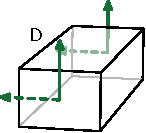
\includegraphics{Blocks/blocks-01}\\ \noindent
  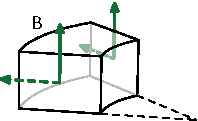
\includegraphics{Blocks/blocks-02}
  \caption{Two \LEGO\ blocks: drift (\ptcelm{D}) and bend (\ptcelm{B}).}
  \label{fig:LEGO.BandD}
\end{marginfigure}

\fref[c]{LEGO.BandD} illustrates these two fundamental types of
\LEGO\ blocks with the entrance and exit reference frames for their
\emph{local} co\"ordinate systems. The solid arrows show the direction
of the local $y$-axes and the dashed arrows show the direction of the
local $x$-axes.
In summary, the bend is characterized by a bending radius $\rho$,
a length $L$, and two faces, each with a reference frame.  The
drift is characterized by a length $L$ and also two faces, each
with a reference frame. The bend is the fundamental block used in
the composition of complex blocks; the drift, of course, is just a
special case of the bend.

\newthought{We are interested} in the deterministic motion through
each \LEGO\ block, represented by the transformation
\begin{equation}\label{eq:zin.zout}
  z_\text{in} \mapsto z_\text{out} = f(z_\text{in}),
\end{equation}
where $f$ denotes a vector of generally nonlinear functions
connecting the local phase-space co\"ordinate $z_\text{in}$
defined in the entrance frame, to the local phase-space
co\"ordinate $z_\text{out}$ in the exit frame. The construction
of such a transformation depends on internal considerations
that are not needed for an understanding of the \LEGO-block
approach. The \LEGO\ block for a single element might, in fact,
comprise a sequence of simpler blocks. This structure, dictated
by the internal geometry of the element, may be hidden.

\begin{marginfigure}[\baselineskip]\forceversofloat
  \centering
  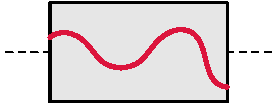
\includegraphics[width=\textwidth]{Blocks/blocks-03}\\[1.5ex]
  
\includegraphics[width=.75\textwidth]{Blocks/blocks-04}
  \caption{Particle trajectories through ``drift'' and ``bend''
           \LEGO\ blocks.}
  \label{fig:LEGO.maps}
\end{marginfigure}
%\begin{figure}[ht]
%  \centering
%  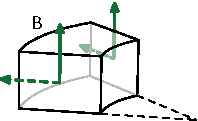
\includegraphics[width=0.6\textwidth]{Blocks/blocks-02}
%  \caption{Particle trajectories through ``drift'' and ``bend''
%           \LEGO\ blocks.}
%  \label{fig:LEGO.maps}
%\end{figure}
In \fref{LEGO.maps} we show a pair of particle trajectories,
in drift and bend \LEGO\ blocks, passing from the entrance face
through to the exit face. As suggested by the trajectories
illustrated, the internal structure may be very complicated
(think of a wiggler); but seen from the outside, our
\LEGO\ blocks are, quite simply, \emph{blocks} with two faces
that define local co\"ordinates with respect to which one may
define $z_\text{in}$ and $z_\text{out}$---\emph{nothing more}.

\index{particle dynamics!local}
\index{element!defined}
\index{beamline element|see{element}}
%
A beamline element is defined by a block with three reference frames,
together with a model, or integrator, which describes how to propagate
a particle from the face with the entrance reference frame to the face
with the exit reference frame:
\begin{equation*}
  \text{element} = \text{block} + \text{model}.
\end{equation*}
The model transforms the phase-space variables from entrance to
exit of the block according to \eqref{zin.zout}. In other words,
it represents the \emph{physics} of the device. Note that the model
also incorporates any approximations we make.

\index{fringe field!magnet}
%
As an example, a block with a bend geometry might actually be a
simple drift, keeping the transverse momenta invariant and
changing only the positions. Or it might be a composition of
blocks describing the body of a magnet and its fringe field
regions. An element might also have non-Hamiltonian effects
such as radiation.%
\footnote{\Aref[c]{states} discusses \PTC's internal state variables,
which describe the characteristic dynamics you can choose for your
accelerator model.}
The list of possible models is endless. In general, a model is
defined by
\begin{itemize}
  \item one or more blocks internal to the model;
  \item a model for each internal block;
  \item the equation of motion in each internal block together with
its integration method and associated number of integration steps.
\end{itemize}

\newthought{In summary}, we define a beamline element locally:
the definition, whether the element is on a work bench or in an
accelerator, is determined solely by the characteristics of that
element. And once we have defined a model for our element, we stick
with it: the \LEGO\ block is inviolate. Like a physical magnet, it
exhibits identical properties under identical conditions.
A significant virtue of our computer-based element, however,
is that it is free to report about what is happening inside.


\subsection{Geometric Transformations}

\index{geometric transformation!defined}
\index{reference frames!connecting}
%
Now that we have defined our two basic types of beamline elements
(drift and bend), the next step is to fit them together. We need
geometric transformations that connect the exit reference frame of
one beamline element to the entrance reference frame of a subsequent
element.

\index{geometric transformation!defined}
\index{LEGO block!analogy}
\index{global frame!described}
\index{global coordinate system!global frame}
\index{layout!global frame}
%
Continuing the \LEGO-block analogy, we put the individual
\LEGO\ blocks on a base, which represents the accelerator model's
\emph{global frame}. Once we know the location of each
\LEGO\ block with respect to the global frame, we know their
locations with respect to to one another.
\fref[c]{LEGO.blocks.base} shows two such \LEGO\ blocks and
their reference frames on a base, which represents the layout of
beamline elements in the global frame of an accelerator. With the
\LEGO\ blocks now on the global frame, we require transformations
that translate the phase-space co\"ordinates in the exit reference
frame of one \LEGO\ block to the phase-space co\"ordinates in the
entrance reference frame of the next \LEGO\ block.
\begin{figure}[ht]\forcerectofloat
  \centering
  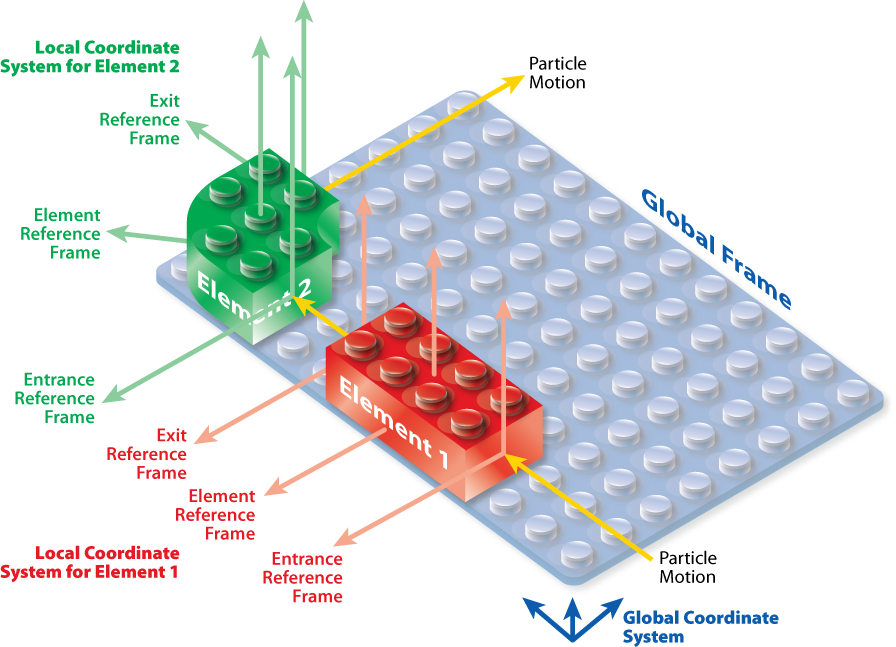
\includegraphics[width=.9\textwidth]{illustrations/LEGO-concept-2}
  \caption{Two \LEGO\ blocks (elements) on a base (global frame).}
  \label{fig:LEGO.blocks.base}
\end{figure}

To construct, for example, a recirculating accelerator out of
\LEGO\ blocks, we connect bends and drifts one after another to
model the desired machine. On reaching the last \LEGO\ block,
we require that the last block's exit face coincide with the
first entrance face. This means that
\begin{itemize}
  \item the blocks' faces must be parallel;
  \item and the frames on the two faces must line up.
\end{itemize}

\begin{marginfigure}[-2.5\baselineskip]
  %\includegraphics[width=\textwidth]{illustrations/connecting-blocks}
  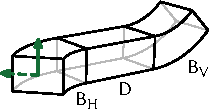
\includegraphics{Blocks/blocks-05}\\
  \noindent\hspace*{.8em}
  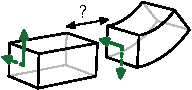
\includegraphics{Blocks/blocks-06}
  \caption{Connecting two horizontal \LEGO\ blocks and a vertical
           \LEGO\ block.}
  \label{fig:connect.blocks}
\end{marginfigure}

\index{patching!defined}
%
Connecting a horizontal bend with a horizontal drift, as for
elements $\text{\ptcelm{B}}_\text{\ptcelm{H}}$ and \ptcelm{D}
in \fref{connect.blocks}, is easy because the $x$- and $y$-axes
of the two elements match. Connecting a horizontal drift with
a vertical bend, as for elements \ptcelm{D} and
$\text{\ptcelm{B}}_\text{\ptcelm{V}}$ in \fref{connect.blocks},
is not as straight-forward: their local $x$- and $y$-axes do not
match. We need, in essence, a new type of
\LEGO\ block---one with an $x$-$y$ rotation of angle $\phi$. (In
\fref{connect.blocks}, of course, $\phi=\ang{90}$.) To build an
arbitrary accelerator, we shall require a full complement of such
additional \LEGO\ blocks.%
\cite[15pt]{Forest:1997:DynEuclid}
This is the subject of \emph{patching}, which uses geometric
transformations to connect the exit frame of one beamline element
to the entrance frame of a subsequent element. Most significantly,
patching enables us to position beamline elements wherever we want
them. We discuss this in more detail later in \TPref*{sec:chart.patch}.

\subsection{Particle Tracking}
\label{sec:ptcl.track}

Now that we have the basic building blocks and the geometric
transformations to fit them together, we can begin to think about
how to track particles. Here we present some essential information
about particle tracking in \PTC.

In keeping with its \LEGO-block philosophy, \PTC\ tracks particles
with respect to \emph{local} frames of reference. The local phase-space
co\"ordinates together with \PTC's knowledge of the local frames
allow the interested user to reconstruct full 3D particle
trajectories with respect to the global frame. In fact, doing exactly
that is useful for checking that one has the constructed the correct
lattice topology in \PTC.

\newthought{Units:} PTC measures all lengths in meters, and all
angles in radians. (It provides the constant \ptc{twopi} to simplify
the conversion from degrees.%
\sidenote{Many other constants are defined in the module
\ptcmod{precision_constants}.})
Particle momenta are scaled by a value $p_o$. This scale momentum
is usually set when defining the lattice (see, for example,
the discussion of \ptc{set_mad} on
\pref{set.mad}). A subtle point involves the fact that the scale
set for one element may differ from that in the preceding element,
\eg\ in the case of acceleration.
In such cases, the patching mentioned above must include not only
geometric transformations, but also energy transformations.

\newthought{Tracking State:} \PTC\ defines a variable
type called \ptctyp{internal_state}.
Objects of this type may be used to modify certain assumptions
\PTC\ makes when it performs tracking. One may, for example,
ask \PTC\ to track only the 4D transverse phase-space variables;
or one may turn on or off radiation. A variable of type
\ptctyp{internal_state}
is essentially a list of flags that one may pass to \PTC\ tracking
routines to modify the algorithms used. For more information, see
\TAref*{states}.

\index{phase space!variables}
\index{variable!phase space}
%
\newthought{Phase-Space Co\"ordinates:} With the default tracking
state, \PTC\ uses the six phase-space variables%
\sidenote{\PTC\ can turn all six of the variables into Taylor series,
or it can omit two of them.  Setting an \ptctyp{internal_state} flag
to ``only four dimensions'' implements the latter behavior.}
\fxnote{Add reference to use of \textsc{only_4d}.}
\begin{subequations}\label{eq:vars.dev}
\begin{equation}\label{eq:vars.dl}
  (x, p_x,\, y, p_y,\, \delta, \ell).
\end{equation}
Here $x$ and $y$ denote the \emph{local} transverse co\"ordinates,
and $p_x$ and $p_y$ denote the corresponding canonical momenta
(divided by a scale momentum $p_o$). The fifth variable, $\delta$,
denotes the relative momentum deviation
\begin{equation*}
 \delta = \frac{p - p_o}{p_o};
\end{equation*}
and the sixth variable, $\ell$, denotes the path-length deviation.%
\sidenote{These last two variables are kept in this order for a technical
reason. This ordering allows us to retain the natural meanings:
positive $\delta$ implies higher energy, and positive $\ell$ implies
longer path length. Because of the Hamiltonian structure, reversing
their order would require us to reverse the sign on one of them.}

One may modify the tracking state so as to change the phase-space
variables. If desired, one may set a flag that causes \PTC\ to compute
flight time rather than path length. In this case, the phase-space
co\"ordinates are
\begin{equation}\label{eq:vars.et}
  (x, p_x,\, y, p_y,\, \varepsilon, ct).
\end{equation}
\end{subequations}
Here the fifth variable, $\varepsilon$, denotes the scaled energy
deviation
\begin{equation*}
  \varepsilon = \frac{E - E_o}{p_o c},
\end{equation*}
where $E_o$ is the energy associated with $p_o$. (In other words, if
$p_o = m c^2 \beta_o \gamma_o$, then $E_o = m c^2 \gamma_o$.) And
the sixth variable, $ct$, is the time-of-flight deviation multiplied by
the speed of light.

One may set a separate flag that causes \PTC\ to compute the total
path length (or flight time) rather than the deviation. In this
case the phase-space variables will be either
\begin{subequations}\label{eq:vars.tot}
\begin{equation}\label{eq:vars.dL}
  (x, p_x,\, y, p_y,\, \delta, L),
\end{equation}
or
\begin{equation}\label{eq:vars.eT}
  (x, p_x,\, y, p_y,\, \varepsilon, cT),
\end{equation}
\end{subequations}
where $L$ and $T$ denote respectively the \emph{total} path length and
\emph{total} flight time.

\begin{marginfigure}[4\baselineskip]\forceversofloat
  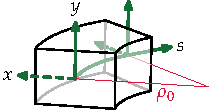
\includegraphics{Blocks/blocks-22}
  \caption{Geometry and local co\"ordinates, $(x,y,s)$, for a
           generic block in \PTC.}
  \label{fig:block.coords}
\end{marginfigure}

\newthought{Hamiltonians:} In accord with its \LEGO-block philosophy,
\PTC\ tracks a particle across an element using a Hamiltonian that is
\emph{local} to that element. The Hamiltonian used by \PTC\ in the body
of an element (no fringe field) then has the simple form
\begin{subequations}\label{eq:Hams}
\begin{equation}\label{eq:Ham.dL}
  - (1 + \kappa_o x) \sqrt{\vphantom{()}\smash{
                           (1 + \delta)^2 - p_x^2 - p_y^2}}
  + (1 + \kappa_o x) \frac{q}{p_o} A_s(x,y)
\end{equation}
if one uses the variables \eqref{vars.dL}, or
\begin{equation}\label{eq:Ham.eT}
  - (1 + \kappa_o x) \sqrt{\vphantom{\frac{1}{1}}\smash{
                           1 + \frac{2}{\beta_o}\,\varepsilon
                             + \varepsilon^2 - p_x^2 - p_y^2}}
  + (1 + \kappa_o x) \frac{q}{p_o} A_s(x,y)
\end{equation}
\end{subequations}
if one uses the variables \eqref{vars.eT}.
Here $\kappa_o = 1 / \rho_o$ denotes
the curvature defined by the \emph{geometry} of the element, and
$A_s$ denotes the longitudinal component of the vector potential.
\fref[c]{block.coords} indicates the variables, including the longitudinal
co\"ordinate $s$. That figure indicates a horizontal bend;
for vertical bends, we do as indicated in the lower part of
\fref{connect.blocks}.
For straight elements, of course, $\kappa_o=0$. If one uses the
variables \eqref{vars.dev}, then there is, effectively, an
additional term that subtracts the default path length or flight
time across that element.\cite{Barber:1994:SpinI}

One may, if desired, have \PTC\ track using an approximation of one of
the Hamiltonians \eqref{Hams} (\ie, using truncated expansions for the
square-root and the vector potential). One might,
for example, do this to speed the computation, but of course the
validity of the expansion for your particular problem should be
verified with careful testing.

\fxnote{Consider using natbib.}
\fxnote{Add reference to \ptc{exact=.false.}}
\fxnote{Add references to use of \textsc{drift_kick_drift} and
\textsc{mad_kind}.}

When integrating across an element described by one of the
Hamiltonians \eqref{Hams}, one typically splits the Hamiltonian
into two integrable pieces.%
\cite{McLachlan:2002:SplitMeth}
If those pieces are, for example, the two terms of \eqref{Ham.dL},
then this is referred to as a \emph{drift-kick} split. Since the
motion of a particle in a uniform dipole is integrable, an
alternative split involves writing $A_s(x,y)$ as a sum of two
pieces: the part that produces a uniform dipole field, and everything
else. Then the dipole field part is added to the drift term of
the Hamiltonian, and we obtain a \emph{bend-kick} split.%
\cite{Forest:1998:BeamDyn,Forest:2006:GeomIntegPA}
One may ask \PTC\ to use one or the other of these splitting methods.

\newthought{Structures for Particles and Beams:} Because \PTC\ tracks particles
with respect to local frames of reference, a set of values for
(as an example) the six phase-space variables \eqref{vars.dl} will not mean
too much unless one knows the context---in particular, where in
the lattice the particle is located. When you need \PTC\ to keep
track of such information for you, it provides some additional
structures. The type \ptctyp{beam} holds an $N\times6$ array for the phase-space
variables, as well as a pointer that tells you where in the lattice
that beam is located. There is also a type \ptctyp{probe} that holds not only
phase-space data, but also data about a particle's spin state.


\subsection{Data Structures for Modeling Accelerator Topologies}

\index{data structure!modeling accelerators}
\index{accelerator topology!simple}
\index{accelerator topology!complex}
\index{topology|see{accelerator topology}}
\index{accelerator!modeling}
\index{modeling!accelerator topologies}
%
\PTC\ data structures fully account for the three-dimensional
structure of a lattice and potential topological complexities
such as those found in colliders and recirculators. In this section,
we discuss a simple lattice and then two complex lattices.

\begin{marginfigure}[0\baselineskip]\forcerectofloat
  \centering
  %\includegraphics[width=\textwidth]{illustrations/model-simple}
  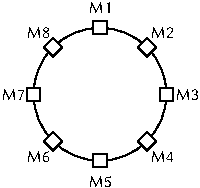
\includegraphics{Layouts/layouts-01}
  \caption{Forward propagation of particles in a circular accelerator.}
  \label{fig:accel.simple}
\end{marginfigure}

\index{forward propagation!example}
\index{propagation|see{backward propagation \emph{or} forward propagation}}
\index{linked list!example for magnets}
%
{A very simple lattice} is shown in \fref[c]{accel.simple},
which illustrates basic forward propagation of particles through a
sequence of magnets%
\marginnote[5pt]{In this discussion, we use the word
``magnet'' whether or not it is actually a magnet, a drift, or any
other beamline element.}
that never varies. Each magnet appears once in the sequence, and
particles go magnet-to-magnet from \ptcelm{M1} through \ptcelm{M8}.
At that point, they re\"enter the magnet \ptcelm{M1}.
A simple linked list of magnets suffices to model this basic topology:
\begin{equation*}
  \text{\ptcelm{ring}} = \text{linked-list}(\text{%
    \ptcelm{M1}, \ptcelm{M2}, \ptcelm{M3}, \ptcelm{M4},
    \ptcelm{M5}, \ptcelm{M6}, \ptcelm{M7}, \ptcelm{M8}}).
\end{equation*}
One might instead use an array of magnets, but that approach
would require us to recreate and reallocate the array whenever
we wish to add or insert a new element. A virtue of the linked
list is that one may easily add or rearrange elements in the
lattice. However, such a simple approach does not suffice when
an accelerator topology reuses the magnets in different sequences,
different directions, or both.

\index{accelerator topology!recirculating}
\index{recirculator!example}
\index{Continuous Electron Beam Accelerator Facility!example based on}
\index{CEBAF|see{Continuous Electron Beam Accelerator Facility}}
\index{Thomas Jefferson National Laboratory!example based on}
\index{JLab|see{Thomas Jefferson National Laboratory}}
%
{To see the difficulties associated with a recirculating beam},
consider \fref[c]{accel.CEBAF}, which shows a machine similar
to the Continuous Electron Beam Accelerator Facility
(\CEBAF) at Thomas Jefferson National Laboratory (\JLab). It
illustrates the concept of particles circulating through a varying
sequence of magnets. The particles start out traveling through an
injector from magnet \ptcelm{M1} through magnet \ptcelm{M4}.
During the first trip circulating around the accelerator, the
particles go through the sequence of magnets \ptcelm{M5},
\ptcelm{M6}, \ptcelm{M7}, \ptcelm{M8}, \ptcelm{M9}, \ptcelm{M10},
\ptcelm{M11}, and \ptcelm{M12}. During their second trip around
the accelerator, the particles go through the sequence of magnets
\ptcelm{M5}, \ptcelm{M6}, \ptcelm{M13}, \ptcelm{M14}, \ptcelm{M9},
\ptcelm{M10}, \ptcelm{M15}, and \ptcelm{M16}. And during their
last trip, the particles go through the sequence of magnets
\ptcelm{M5}, \ptcelm{M6}, \ptcelm{M17}, \ptcelm{M18}, \ptcelm{M9},
and \ptcelm{M10}.  The particles are then dumped. Note that magnets
\ptcelm{M5}, \ptcelm{M6}, \ptcelm{M9}, and \ptcelm{M10} appear in
all three circuits.

\begin{figure}[ht]
  \centering
  %\includegraphics[width=.9\textwidth]{illustrations/model-JLAB}\\
  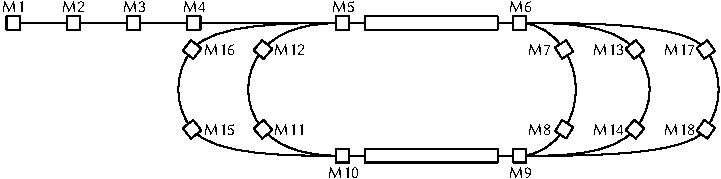
\includegraphics{Layouts/layouts-02}
  \caption{A recirculator illustrates particles traveling
           through a varying sequence of magnets.}
  \label{fig:accel.CEBAF}
\end{figure}

A linked list of \emph{magnets} cannot properly represent the
physics of this situation. In a linked list, magnet \ptcelm{M6},
for example, must point to only one magnet. It cannot point to
\ptcelm{M7}, \ptcelm{M13}, \emph{and} \ptcelm{M17} unless we
create two clones of \ptcelm{M6}. Creating clones, however, is
a bad idea: If we wish to adjust the position or strength of
magnet \ptcelm{M6}, such adjustments would have be made three
times: once in the magnet itself, and once in each of its two
clones.

\index{linked list!example for fibres}
\index{fibre!defined}
%
A better solution separates the magnets from the linked list that
tracks the path of particles through the magnets. \PTC\ does this
with a linked list of containers called \emph{fibres}, each with
a pointer to the appropriate magnet. Adjustments to the position
or strength of a magnet are made once and are automatically taken
into account each time a container in the linked list points to
that magnet. We discuss the linked list of containers with pointers
to magnets in \TSref*{accel.topo}.

\begin{figure}[ht]
  \centering
  %\includegraphics[width=.65\textwidth]{illustrations/model-RHIC}
  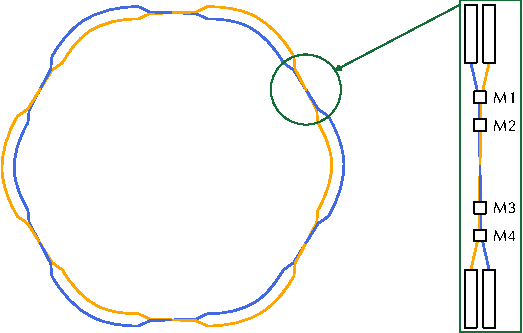
\includegraphics{Layouts/layouts-06}
  \caption{Particles circulating in different directions
           through an accelerator.}
  \label{fig:accel.RHIC}
\end{figure}

\index{accelerator topology!collider}
\index{collider!example}
\index{Relativistic Heavy Ion Collider!example based on}
\index{RHIC|see{Relativistic Heavy Ion Collider}}
\index{Brookhaven National Laboratory!example based on}
\index{forward propagation!example}
\index{backward propagation!example}
%
What about a collider? \fref[c]{accel.RHIC}, based on the intersecting
rings of the Relativistic Heavy Ion Collider (\RHIC) at Brookhaven
National Laboratory (\BNL), shows particles circulating in both
directions (forward and backward propagation) through some of the
same magnets. For example, the particles following the blue path go
though one set of magnets in the sequence \ptcelm{M1}, \ptcelm{M2},
\ptcelm{M3}, \ptcelm{M4}. Meanwhile, the particles following the
yellow path traverse the same set of magnets in the reverse order:
\ptcelm{M4}, \ptcelm{M3}, \ptcelm{M2}, \ptcelm{M1}.

\index{linked list!example for fibres}
%
Using an array or a linked list with clones of magnets creates
the same problems as before, and \PTC\ alleviates the difficulties
by using doubly-linked lists%
\marginnote{The use of a \emph{doubly}-linked list enables both
forward and reverse propagation through a given sequence of
beamline elements.}
of containers that follow the particle
paths---containers which have inside them pointers to the appropriate
magnets. Changes to the strength or position of, say, magnet
\ptcelm{M3} are made once in the object for magnet \ptcelm{M3} and
are immediately reflected in the two linked lists---one linked list
for each of the two particle beams.


\section{Modeling Accelerator Topologies}
\label{sec:accel.topo}

\index{accelerator!modeling}
\index{modeling!accelerator topologies}
%
\glossary{accelerator topology}{A description in spatial terms of
the magnets in an accelerator and how they interact with particles.}
%
To set up a linked list of containers with pointers to the elements
in a beamline, \PTC\ employs three different data types:
\ptctyp{element}, \ptctyp{fibre}, and \ptctyp{layout}.
\PTC\ also provides what it refers to as a \emph{\DNA\ database},
which one may populate with \ptctyp{layout}s that one may use to
construct complex accelerator topologies. Finally, for the proper
positioning of elements in the accelerator, \PTC\ uses two additional
data types: \ptctyp{chart} and \ptctyp{patch}. We discuss all these
concepts in this section.


\subsection{Element}

\index{element!defined}
\index{data type!\ptc{ELEMENT}}
\index{ELEMENT@\ptc{ELEMENT}!data type}
\index{type|see{data type}}
%
The data type \ptctyp{element} represents a beamline element in a
machine. It contains information about the element type (dipole,
quadrupole, rf cavity, \etc), its physical properties (length,
strength, \etc), and its location and orientation in space.  In
\PTC, it is the fundamental object. \PTC\ preserves each element's
physical and mathematical integrity to ensure that it can be
positioned, repositioned, or misaligned \emph{as a whole}. At the
same time, \PTC\ provides the capability for one to look inside the
element to see, for example, details of a particle trajectory. One
should therefore \emph{never} feel compelled to split an element in
half. \et{In \PTC\ one can simply choose an even number of integrations steps; the code automatically sets up a pointer called tm that points to the center of the magnet. }

In addition to information about the element itself, the data type
\ptctyp{element} includes information about which \ptctyp{fibre}s
point to it. This information is used by \PTC\ to ensure that if
an element is moved, then all beamlines containing it know about
the move.

%As in a real machine, the same element may appear in several
%beamlines, or it may reappear in the same recirculating beamline
%several times.


\subsection{Fibre}
\fxnote{Add margin note re origin of term \emph{fibre}.}

\index{fibre!defined}
\index{data type!\ptc{FIBRE}}
%
The data type \ptctyp{fibre} contains a pointer to a beamline
element as well as pointers to the fibres that precede and follow
it along a particle path. When strung together in a linked list,
a sequence of fibres defines a beamline. The fact that different
fibres can point to the same element means that separate beamlines
can share common elements; and this gives \PTC\ the capability to
model complex accelerator topologies.

\index{chart!defined}
\index{patch!defined}
%
A \ptctyp{fibre} contains, among other items,
\begin{itemize}
  \item a pointer to an \ptctyp{element};
  \item pointers to the previous and next \ptctyp{fibre}s
        along a beamline;
  \item a pointer to a \ptctyp{chart} that locates the element
        within the global reference frame;
  \item a pointer to a \ptctyp{patch} that connects the elements
        of successive fibres geometrically, energetically, and
        temporally;
  \item the \emph{direction of propagation} through the element.
\end{itemize}


\subsection{Layout}

\index{layout!defined}
\index{beamline!defined as layout}
\index{data type!\ptc{LAYOUT}}
%
The data type \ptctyp{layout} represents a beamline as a doubly-linked
list of \ptctyp{fibre}s. It follows the particle path by specifying
the order of the fibres, which each point to an actual element in
the beamline.%
\sidenote{Note that a \ptctyp{layout} need not represent an entire
machine: it may represent just a piece of an machine. The full
accelerator would then be built from several layouts.}
In addition, a \ptctyp{layout} defines the direction of
propagation through the sequence of fibres and whether the particles
recirculate.

\begin{figure}[ht]%\forcerectofloat
  \centering
  %\includegraphics[width=.9\textwidth]{illustrations/model-JLAB-fibres}
  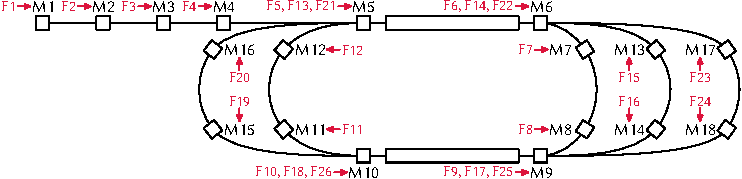
\includegraphics{Layouts/layouts-03}
  \caption{A layout with a linked list of fibres pointing to magnets.}
  \label{fig:CEBAF.layout.fibres}
\end{figure}

As an example,%
\marginnote{As before, we say ``magnet'', but it may mean any type
of beamline element.}
consider the accelerator illustrated in
\fref{accel.CEBAF}. We could construct it as indicated in
\fref{CEBAF.layout.fibres}, which shows a \PTC\ \ptctyp{layout}
with a linked list of 26 fibres (\ptcelm{F\#}) pointing to the
18 magnets (\ptcelm{M\#}).

\index{DNA database!defined}
\index{database|see{DNA database}}
\index{DNA sequence!defined}
\index{sequence|see{DNA sequence}}
\index{DNA|see{DNA array, DNA database, \emph{or} DNA sequence}}
%
\newthought{Most accelerator modeling codes} do not, as \PTC\ does,
enforce a dichotomy between fibres and elements. As a consequence,
it can be difficult to import lattice descriptions from other codes
into \PTC\ in a manner consistent with \PTC's approach to modeling
accelerators. To overcome this difficulty, \PTC\ provides what it
refers to as a \emph{\DNA\ database}. This database is first
populated with a set of \ptctyp{layout}s whose fibres point to
unique elements.  In other words, no element appears more than
once---via the fibres---in the set of \DNA\ layouts. (This much may,
if desired, be done by importing from an external lattice description.)
These simple layouts---we shall refer to them as
\emph{\DNA\ sequences}---may then be used to construct complex layouts
of the form shown in \fref{CEBAF.layout.fibres}.

\begin{marginfigure}[-2\baselineskip]
  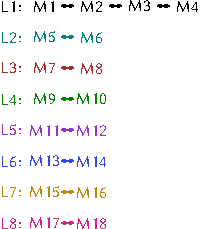
\includegraphics{Layouts/layouts-04}\vspace{5pt}
  \caption{DNA database with eight DNA sequences (\ptcelm{L1}
           through \ptcelm{L8}). The arrows represent the links in
           the doubly-linked list of fibres that constitutes a layout.
           Each fibre points to (contains) the indicated magnet
           (\ptcelm{M1}--\ptcelm{M18}).}
  \label{fig:DNA.database}
\end{marginfigure}
%
\index{layout!non-trackable}
%
As a concrete example, consider how we might do this for the
accelerator shown in \fref{accel.CEBAF} or \fref*{CEBAF.layout.fibres}:
We first create a set of layouts in which no magnet appears
twice, and which have no magnets in common. The logical course
in this case is to create the eight layouts \ptcelm{L1} through
\ptcelm{L8} shown in \fref{DNA.database}. Note that each of the
eighteen magnets appears just once in this database. Here we show
each of the \DNA\ sequences in a different color; and these colors
match those used in \fref{CEBAF.DNA}, which shows the accelerator
with the different \DNA\ sequences indicated by the corresponding
colors.

\begin{figure}[ht]%\forceversofloat
  \centering
  %\includegraphics[width=.9\textwidth]{illustrations/model-JLAB-DNA}
  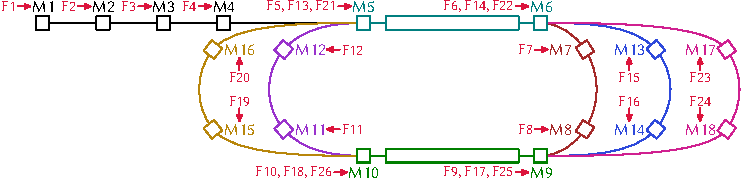
\includegraphics{Layouts/layouts-05}
  \caption{Eight layouts or DNA sequences.}
  \label{fig:CEBAF.DNA}
\end{figure}

\index{layout!trackable}
%
Having created the eight \DNA\ sequences in our \DNA\ database,
we can now use \PTC\ to string these basic layouts together to
create the \emph{trackable layout} that represents the full machine
illustrated in \fref{accel.CEBAF}, or \fref*{CEBAF.layout.fibres}
or \fref*{CEBAF.DNA}. Evidently, a trackable layout may be constructed
from one or more \DNA\ sequences.%
\sidenote{By contrast, we may sometimes refer to the
\DNA\ sequences---high-level building blocks of our accelerator
model---as \emph{non-trackable layouts}.}

In general, once we have populated the \DNA\ database (either
from within \PTC\ or by importing external lattice descriptions) we
can use \PTC\ to string together these basic layouts to create
the additional layouts we need for tracking. These latter---\ptcelm{T1}
through \ptcelm{TN}, say---contain fibres that point to elements
in the \DNA\ database. For the recirculator shown in
\fref{accel.CEBAF}, we would create one beamline layout \ptcelm{T1}
with 26 fibres, each pointing to an element in the \DNA\ database.
For the collider shown in \fref{accel.RHIC}, we would create two
beamline layouts, \ptcelm{T1} and \ptcelm{T2}, one layout for
each ring.


\subsection{Chart and Patch}
\label{sec:chart.patch}

\index{patching!reference frames}
\index{reference frame!patching}
\index{geometric transformation!patching}
\index{tracking!automatic}
%
\PTC\ uses  the new data types \ptctyp{chart} and \ptctyp{patch}
to locate, connect, and move the elements of a beamline. The
generic capability, which we term \emph{patching}, connects the
exit frame of one element to the entrance frame of the subsequent
element.

\index{chart!defined}
\index{chart!contains misalignment}
\index{data type!\ptc{CHART}}
%
The data type \ptctyp{chart} contains a pointer to a frame of
reference (actually the collection of three frames illustrated in
\fref{LEGO.element}) that locates a fibre (really the element the
fibre points to) within \PTC's global three-dimensional reference
frame. The chart also contains information that describes, if present,
any misalignment of the fibre.

\index{patch!defined}
\index{data type!\ptc{PATCH}}
%
The data type \ptctyp{patch} contains information about the
about the relation between the exit reference frame of one
element and the entrance reference frame of the subsequent
element. As a consequence, a \ptctyp{patch} is a property not
of an \ptctyp{element} but of a \ptctyp{fibre}, and it must
be computed \emph{after} placing both elements in their final
locations.

As a concrete example, consider the set of elements illustrated
in \fref{patch.elems}. There we see three elements separated by
a pair of drifts. We know the locations of these elements
(in particular the reference frames attached to these elements)
because of the information stored in the corresponding charts.
The second drift is explicitly defined as the third beamline
element. The first drift, however, is not explicitly defined.
The exit frame of element~1 and the entrance frame of element~2
do not coincide, and this indicates the need for a patch. The
remaining elements all have exit-entrance frame pairs that
coincide, and hence no additional patches are required.

\begin{figure}[ht]%\forcerectofloat
  \centering
  %\includegraphics[width=.9\textwidth]{illustrations/patching-element}
  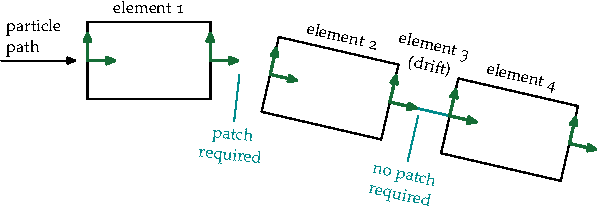
\includegraphics{Patches/patches-01}
  \caption{Patching elements in a single beamline.}
  \label{fig:patch.elems}
\end{figure}

\index{recirculator!patching beamlines}
%
As another example of patching, \fref{patch.recirc} shows three
magnets in a recirculator. A high-energy particle passing through
magnet~1 follows the red trajectory to magnet~2. After exiting
magnet~2, the particle continues around the machine and returns
with a lower energy (after deceleration by appropriately phased
rf fields) to magnet~1. Because the particle has less energy,
magnet~1, the separator, now bends it along the blue trajectory
towards magnet~3, the first magnet in a new beamline.
Magnet~1 of \fref{patch.recirc} must, of course, appear in two
fibres: the first points to magnet~2 as the subsequent element,
while the second points to magnet~3. What about the patches?
Assuming the exit frame of magnet~1 and the entrance frame of
magnet~2 have the same unit vectors but different origins. then
the patch between the fibres pointing to magnets 1 and 2 must
correspond to a simple drift of the appropriate length---and that
is exactly what \PTC\ will compute. The patch between the fibres
pointing to magnets 1 and 3 corresponds to three actions: a drift
of length $d$, a co\"ordinate frame rotation by angle $\alpha$,
and a translation of length $h$.

\begin{figure}[ht]
  \centering
  %\includegraphics[width=.7\textwidth]{illustrations/patching-beam-lines}
  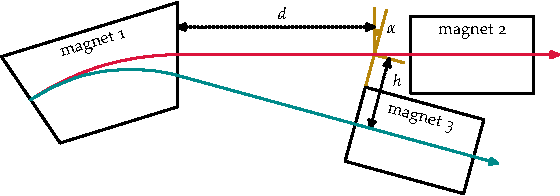
\includegraphics{Patches/patches-02}
  \caption{Patching elements in multiple beamlines.}
  \label{fig:patch.recirc}
\end{figure}


\subsection{Misalignments}

\index{misalignment!described}
%
The accelerator we design is never the one we build. This fact
makes it essential to investigate the margin for error in any
design. To simulate misalignment errors, \PTC\ uses the approach
illustrated in \fref{misalignment}. There we show the original
element~2 with a light gray outline, and the misaligned element~2
with a red outline. To push a particle from the exit of element~1
to the entrance of element~3, \PTC\ first applies the patch from
element~1 to the original element~2. Then \PTC\ traverses element~2
in three steps: an entrance misalignment, the standard element~2,
and an exit misalignment.
\PTC\ then applies the patch from element~2 to element~3.
If we remove the misalignment (which translates and rotates element~2),
the element returns to its design position in the fibre.

\begin{figure}[ht]%\forceversofloat
  \centering
  %\includegraphics[width=.9\textwidth]{illustrations/misaligning-element}
  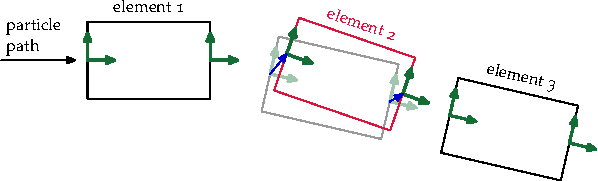
\includegraphics{Patches/patches-03}
  \caption{Misaligning an element.}
  \label{fig:misalignment}
\end{figure}


\section{Analyzing an Accelerator to Understand its Properties}
\label{sec:analyze.accel.prop}

\index{accelerator!analysis}
\index{accelerator!properties}
\index{property!accelerator}
%
In this overview chapter, the first two sections,
\Tref{sec:track.ptcl.accel} and \Tref{sec:accel.topo}, discuss
the essential concepts and data structures used by \PTC\ to
construct a computer model of an accelerator and simulate particle
trajectories through that model. Your next activity is likely to
be that of asking questions of your simulated accelerator: Where
is the particle in that magnet? What are the Twiss parameters at
this location in the ring? What are the horizontal and vertical
tunes of this machine? How much synchrotron radiation does my
particle emit while traversing this magnet? Such questions are
the domain of \emph{analysis}.

\index{map-based methods!global}
%
At the heart of the software design decisions made for \PTC\ lies
the desire to analyze \emph{real} accelerators. The fact that real
accelerators are complicated beasts---with many individual magnets
performing many individual functions---leads directly to \PTC's
simulating accelerators using the \LEGO-block approach, which
emphasizes a \emph{local} view of beamline elements and particle
tracking. Similarly, the desire to analyze leads directly to \PTC's
use of map-based methods, which emphasize a \emph{global} view of
the accelerator.

\index{map-based methods}
\index{one-turn map}
\index{perturbation theory!derived via one-turn map}
%
Map-based methods are fundamental to the analysis of real
accelerators. Think of a one-turn map as a piece of sophisticated
diagnostic hardware that you install at some point in the ring.
It enables you to observe the beam turn after turn. It follows that
any \emph{sensible} question you might ask about the beam at that
point in the ring must be contained within that one-turn map.
Indeed, all of standard perturbation theory may be expressed
entirely in terms of the one-turn map.\cite{Forest:1990:HamFree}

If you desire information at some other point in the ring, then
you must, of course, install another sophisticated beam monitor
at that new location. Using map-based methods, this will be
equivalent to a proper combination of the one-turn map at your
original location and the transfer map that connects the two
locations of interest. As a consequence, a one-turn map plus
partial-turn transfer maps contain the answers to all sensible
questions you might ask of an accelerator model.

\index{one-turn map!analysis independent of construction}
%
The analogy of a one-turn map as a sophisticated beam monitor
also implies---quite correctly---that no connection exists
between the \emph{construction} of a one-turn map and its
\emph{analysis}. The construction is done using a strictly
local approach, which is our only hope of getting the physics
right in this complicated and messy world. Once we've obtained
the one-turn map, we may forget where it came from and what
various frames of reference were used to compute it. We now
concentrate on asking sensible questions of our ``beam monitor''.


\subsection{Local versus Global Information}

\index{local information!analysis}
\index{global information!analysis}
\index{property!local}
\index{property!global}
\index{local information|see{\emph{also} local property}}
\index{global information|see{\emph{also} global property}}
%
\PTC\ provides you with two kinds of information: local and global.

\index{local information!defined}
%
Information about an element, or a particle in an element,
is called \emph{local} if it can be obtained independently of
any knowledge of the element's position in an accelerator.
It could be obtained even if the element were a prototype
sitting on a test bench in your lab. The field strength at
a particular location in the element is an obvious example
of local information. Another example is a particle's
trajectory through a magnet: When, for example, an electron
appears at the entrance of a quadrupole, we can predict its
(local) trajectory without any knowledge of where the electron
came from, or where it is going. Yet another example of local
information is the amount of synchrotron radiation emitted by
a particle as it traverses a magnet.

\index{global information!defined}
%
Information is called \emph{global} if it can be obtained
only after constructing an accelerator. The dynamic aperture
is an example of global information, because it makes sense
only in the context of circulating particles around an
accelerator ring. Other examples include\\
%\vspace{-\baselineskip}
\begin{tabular}{lll}
  tune          & closed orbit            & normal mode decomposition \\
  tune shift    & resonance               & damping partition number \\
  chromaticity  & linear lattice function & nonlinear distortion
                                               function \\
  anharmonicity & equilibrium emittance   & short-, mid-, and
                                               long-term stability
\end{tabular}\\
%\vspace{-\baselineskip}
\noindent and much more.

Note that all local quantities are governed solely by the
particulars of an element and the underlying equations of
motion. Particle information, local field strengths, and the
Lorentz equation are all you need to know for the computation
of local quantities. Global quantities, on the other hand,
are governed by the fact that an accelerator ring is designed
to circulate particles in stable orbits for many turns. They
result from our efforts to \emph{interpret} the one-turn map.


\subsection{Polymorphs and Normal Form}

The simplest simulation of particle trajectories in an accelerator
represents a particle as an array $z$ of real numbers, which
constitutes the phase-space co\"ordinates and any other quantities
(spin, for example) that need to be tracked. One then tracks the
particle through the accelerator by integrating the appropriate
equations of motion with initial conditions given by $z^i$. If we
wish to know the behavior of nearby particles, then we could, of
course, launch other particles with initial conditions $z^i+\varepsilon$
and study how the results vary with $\varepsilon$. What we want,
then, is a functional representation of the behavior near $z^i$
using, for example, a Taylor series. Moreover, it will be convenient,
indeed desirable, if we can switch between the real or Taylor series
representations at runtime. To achieve this, \PTC\ defines the
variable type \ptctyp{real_8}, which holds containers for a real,
a Taylor series, and other information, as well as a flag that
allows the user to set the representation. This \ptctyp{real_8}
is a so-called \emph{polymorphic} variable. With this polymorphism,
\PTC\ gives us access to all of standard perturbation theory,
including the kinds of global information mentioned above.
To make the most effective use of polymorphism, \PTC\ also overloads
the standard mathematical operators so that algorithms written for
reals immediately apply to Taylor series and any other representations
held by the type \ptctyp{real_8}.

As indicated above, rather than propagating a particle,
\ie\ a \ptctyp{real}, through an accelerator, one may instead wish
to propagate a \emph{neighborhood}, \ie\ an array of truncated power
series (\TPS) that represents the particle and its phase-space
neighborhood. Given a software library that implements a truncated power
series algebra (\TPSA), one can use polymorphism and operator
overloading to turn any single-particle tracking algorithm into a
map generation algorithm.
The polymorphism of \PTC\ makes it possible to to compute transfer
maps in a transparent manner.
%The result
%of such tracking is a one turn map for that region of phase space.

\index{SDGQ@\SDGQ\ ($s$-dependent global quantity)}
\index{$s$-dependent global quantity!defined}
%
\newthought{The concept of a {normal form}} is absolutely central
to the modern view of accelerator analysis. In the very simplest
case, a one-turn map reduces to a matrix $M$, and we factor it in
the form of a similarity transformation:
\begin{equation*}
  M = A \cdot N \cdot A^{-1}.
\end{equation*}
Here $N$ denotes a \emph{normal form}, and $A$ denotes the matrix
that transforms between $N$ and $M$. Continuing our simplest example,
$N$ generates rotations in each of the separate phase planes,
and $A$ converts the circles of normal form co\"ordinates to
generic phase-space ellipses. If we go to another location in the
accelerator, the one-turn map will differ, but it will have the
same normal form:
\begin{equation*}
  M' = A' \cdot N \cdot A'^{-1}.
\end{equation*}
In other words, $N$ is an invariant of the ring.
Global scalars, by which we mean global quantities that do not
depend on location around the accelerator, may be derived from
$N$. The $s$-dependent global quantities (\SDGQ{}s) may be derived
from the transformations $A$, $A'$, \dots.
Thus, for example, one extracts tunes from $N$ and linear lattice
functions from the $A$s.

Two very important benefits derive from a normal form factorization
of the one-turn map: The first benefit is that this factorization
generalizes in a straightforward manner to nonlinear maps. We may
thus write the map $M(z)$ as the composition
\begin{equation}\label{eq:M.ANAi}
  M(z) = A \circ N \circ A^{-1}(z),
\end{equation}
where now $M$, $A$, and $N$ all denote nonlinear functions on phase
space. As in the matrix case, the normal form $N(z)$ yields the
global scalars, and the transformation $A(z)$ yields the \SDGQ{}s.
$N$, for example, contains not only the tunes, but also the nonlinear
information of how the tunes vary with amplitude. The second benefit
is that we may use the \emph{same code} that produced the one-turn
map $M(z)$ to propagate the normalizing transformation $A(z)$. Doing
exactly this---using the polymorphic capabilities of \PTC, of
course---we can compute \SDGQ{}s at many locations around the ring.

As with all things wonderful, some caveats attach to the normal
form decomposition \eqref{M.ANAi}. The first caveat is associated
with the approximate nature of the work we do. Unless our system
is extremely special, we can know $M(z)$ only up through some
finite order. Moreover, because of the complicated nature of
particle orbits in accelerators, the expansion is generally
asymptotic. As a consequence, we should examine all analyses in
the light of common sense and actual particle tracking.%
\sidenote{This should \emph{already} be part of your routine.}

The second caveat is associated with the fact that the
transformation $A(z)$ is not unique: If $B$ denotes any
transformation that commutes with $N$, then replacing $A(z)$ in
\eqref{M.ANAi} with $A \circ B(z)$ yields the same result. In
other words, the particular $A$ we choose to work with depends on
certain conventions. For physical quantities associated with $A(z)$,
this freedom in the definition of $A$ necessarily has no effect. But
some quantities%
\sidenote[][-2\baselineskip]{One example is the so-called phase
advance. Consider two locations in the ring that have identical
one-turn maps. At such so-called \emph{matched} locations in a ring, the normalizing
transformations (chosen with common conventions!) are identical;
as a consequence, the phase advance between such locations is
well-defined. Between \emph{un}matched locations, however, the
definition of phase advance can depend on the conventions used in
extracting the $A$s.}
that people discuss \emph{do}, in fact, depend on the particular
choice for the normalizing transformation $A$. Such quantities,
needless to say, cannot be physical and should be used with great
care, or not at all.\cite{Chao:2008:SLIMrevisted}


\section{Modeling Particle Interactions}
\label{sec:ptcl.intxns}

\index{particle!interaction}
\index{modeling!particle interactions}
%
This overview chapter has, until now, discussed concepts related
to single-particle dynamics. In this section we introduce some
concepts related to the inclusion of particle interactions in
\PTC\ simulations. Some of these concepts, however, apply also
to single-particle dynamics, and hence we urge even readers not
interested in space-charge to at least skim this section.

We begin with a caveat: \emph{The inclusion of particle
interactions violates the philosophy of \PTC.} To see
this, consider a beam of self-interacting particles at
a moment when the head has entered a magnet and the tail
has not. Particles in the head and tail communicate via
the self interactions, and hence the dynamics of particles
in the head and tail affect one another. If we place the
magnet in a different location, particles in the head will
follow different trajectories. The particle interactions
communicate this information to the tail, and now particles
in the tail also follow different trajectories---their
behavior differs because of a change in a magnet they have
yet to see. This scenario tells us that if our beam is
spatially extended and self-interacting, we cannot define
an isolated propagator for each element. In other words,
particle interactions violate the \LEGO-block approach to
modeling accelerators.

To fit within the philosophy of \PTC, beamline elements must
be independent of one another. This idealization---upon which
most tracking codes rely---should be borne in mind when using
\PTC---or any of those other codes---to simulate beams with
self-interacting particles.%
\sidenote{Overlapping fringe fields also violate the principle
of magnet independence; and in that case, too, one must exercise care.}

In the rest of this section, we discuss some of the data
types useful for including particle interactions:
\ptctyp{integration_node}, \ptctyp{node_layout}, \ptctyp{probe},
and \ptctyp{temporal_probe}. We also describe the basic idea
behind the time-based tracking capability of \PTC.


\subsection{Integration Node}
\label{sec:integr.node}

\index{integration node!defined}
\index{data type!\ptctyp{integration_node}}
\index{element!composed of integration nodes}
\index{node|see{integration node}}
\index{entrance patch!integration node}
\index{entrance fringe field!integration node}
\index{exit patch!integration node}
\index{exit fringe field!integration node}
\index{fringe field!integration node}
%
The data type \ptctyp{integration_node} represents a step of
integration in \PTC. In particular, this data type includes
entrance and exit reference frames, pointers to the previous
and next integration nodes along a particle path
(see \Tref{sec:node.layout}), and a pointer to the parent
\ptctyp{fibre} that contains it. Integration nodes allow us to
examine data inside a beamline element without violating the
element as a fundamental unit---a self-contained \LEGO\ block.
They allow us to resist the temptation to ``slice'' an element
by hand: they \emph{are} the slices. The data type
\ptctyp{integration_node} also contains an integer that
determines the \emph{type} of integration node, of which there
are five. See \fref{integr.nodes}. On traversing the integration
nodes that represent an element, one encounters, in order,
\begin{itemize}
  \item an entrance patch (and misalignment, if any), which
connects the geometry described by the fibre to that of the
preceding fibre in the linked list;
  \item an entrance fringe field, which contains approximate
fringe effects (if any);
  \item $N$ body integration nodes representing the body of element;%
\footnote{The choice of $N$, which you are free to modify,
obviously affects the accuracy of your simulation.
\Cref[c]{symplectic.integ} discusses how to split elements into
integration nodes.}
  \item an exit fringe field, which contains approximate fringe
effects (if any);
  \item an exit patch, which connects the geometry described by
the fibre to that of the following fibre in the linked list.
\end{itemize}



\begin{figure}[ht]
  \centering
  %\includegraphics[width=.9\textwidth]{illustrations/integration-nodes}
  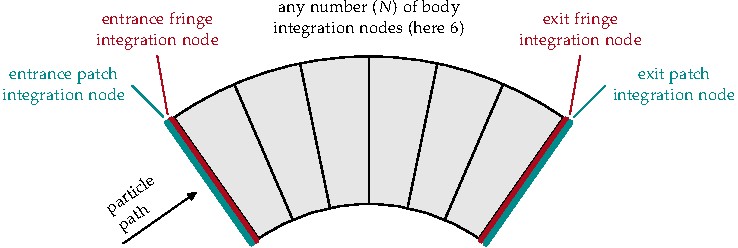
\includegraphics{Elements/nodes-01}
  \caption{$N+4$ integration nodes cover an element.}
  \label{fig:integr.nodes}
\end{figure}

\index{s-based tracking!integration node}
\index{time-based tracking!integration node}
%
Using $s$-based tracking, we can obtain particle data at the
entrance and exit of each integration node in the body of a
magnet, that is, at the seven black lines in \fref{integr.nodes}.
In addition, we can obtain first-order information about the location
within a node of a particle at some fixed time
(see \Tref{sec:pseudo.time}).

The integration nodes \emph{contain no duplicate data about
the elements}; they have no existence apart from the beamline
elements they represent. Because the data in the integration
nodes reside on the fibres (which point to the elements),
\PTC\ is able to carry over changes affecting elements
(\eg, a change in the magnetic field) and changes affecting
the fibres (\eg, misalignments) to the integration nodes.


\subsection{Node Layout}
\label{sec:node.layout}

\index{node layout!defined}
\index{data type!\ptc{NODE_LAYOUT}}
\index{layout|see{\emph{also} node layout}}
\index{linked list!integration nodes}
\index{beamline!expanded}
%
\fxnote{Should have some comment, probably later about
\ptctyp{node_layout} inserting a bunch of additional reference
frames.}
%
The data type \ptctyp{node_layout} represents a beamline as a
linked list of \ptctyp{integration_node}s. It includes pointers
to the first and last integration nodes in the beamline, as well
as a pointer to the parent \ptctyp{layout}. To access the
integration nodes of a particular fibre, one may step through
them, making use the fact that the data type \ptctyp{fibre}
includes pointers to the first, last, and middle integration nodes
for the corresponding element.

A \ptctyp{node_layout} is not created automatically when you
create a \ptctyp{layout}: You must ask \PTC\ to create it and
populate the associated reference frames.
\fxnote{Add reference to example(s).}


\subsection{Probe and Temporal Probe}

\index{probe!defined}
\index{data type!\ptctyp{probe}}
%
The data type \ptctyp{probe} represents a particle. In particular,
it contains, for a given particle, both the orbital phase-space data
and a \ptctyp{spinor} for the spin data. Should the particle become
lost, the \ptctyp{probe} contains a \ptctyp{logical} in which to
record this fact, as well a pointer to the \ptctyp{integration_node}
in which the particle loss occured.

\index{temporal probe!defined}
\index{data type!\ptc{TEMPORAL_PROBE}}
\index{probe|see{\emph{also} temporal probe}}
%
The data type \ptctyp{temporal_probe} contains a \ptctyp{probe}
together with information relevant to the time-based tracking
capability of \PTC. This includes a pointer to the
\ptctyp{integration_node} that currently contains the particle.


\subsection{Time-based Tracking}
\label{sec:pseudo.time}

\index{time-based tracking!integration node}
\index{time-based tracking!described}
%
Any high-order $s$-based integrator may be converted to a
first-order time-based integrator \emph{provided information
is available about the three-dimensional environment.} When
we ask \PTC\ to perform time-based tracking, \PTC\ augments
its $s$-based information with temporal information. \PTC's
tracking remains fundamentally $s$-based, but with the
additional information, it can determine which integration
node a particle is in at a given time. \PTC\ can
then compute a first-order accurate location inside that node
for the particle at that time.

\begin{figure}[ht]
  \centering
  %\includegraphics{illustrations/space-charge-kick}
  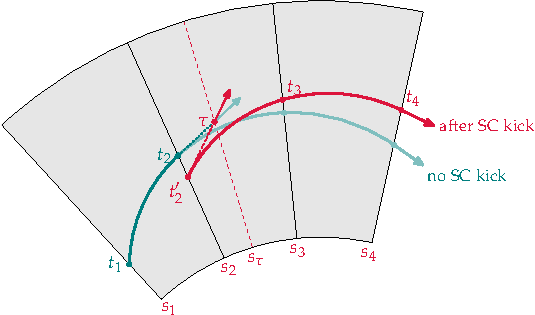
\includegraphics{Elements/nodes-02}
  \caption{Applying a space-charge kick at time $\tau$.}
  \label{fig:sc.kick}
\end{figure}

\index{space-charge kick!used with time-based tracking}
\index{kick!space-charge}
\index{particle!space-charge kick}
\index{particle!interaction}
\index{space-charge kick!applying}
%
\PTC's time-based tracking capability allows us to obtain a
snapshot of the beam at a fixed time. \fref[c]{sc.kick}
illustrates this approach to applying a space-charge kick at
time $\tau$:
\begin{enumerate}
  \item \PTC\ checks node by node the entrance and exit times
of a particle to determine the integration node for which
$\tau \in [t_\text{entrance},t_\text{exit})$. After locating
the appropriate node, \PTC\ returns the particle to the node
entrance. At this point in \fref{sc.kick}, because $\tau$ falls
between times $t_2$ and $t_3$, the particle is on the blue curve
at the point labeled with time $t_2$.
  \item \PTC\ determines the time difference
$\delta t = \tau - t_\text{entrance}$. Then, using the particle's
position and momentum at the node entrance as an initial condition,
and assuming the current integration node to be a drift,
\PTC\ computes a position and momentum for the particle at time $\tau$.
It records the shift $\delta s$ in the \ptctyp{temporal_probe}.
If the element \emph{is} a drift, the position of the particle at
time $\tau$ is exact. If the element is \emph{not} a drift, the
position of the particle at time $\tau$ is a close approximation.
At this point in \fref{sc.kick}, the particle is at the point
labeled with time $\tau$.
  \item After completing the above two steps for all particles in
the beam, you can apply space-charge kicks to your particles. At
this point in \fref{sc.kick}, the particle remains at the point
labeled with time $\tau$, but it has a new momentum, as indicated
by the angle between the light blue arrow and the red arrow.
  \item \PTC\ now drifts the particle---with its new momentum---back
to the entrance of the integration node. At this point in
\fref{sc.kick}, the particle is back in the $s_2$ plane, but now
on the red curve at the point labeled with time $t_2'$.
  \item \PTC\ now continues tracking the particle---with its new momentum---seeking the integration node for which $t_\text{entrance}$ and $t_\text{exit}$ bracket the time for the next space-charge kick.
\end{enumerate}

\endinput
 % overview
%!TEX root = ../PTC-LibUG.tex
\linenumberfrequency{5}

\chapter{Modeling an Accelerator with \PTC}
\label{cha:model.accel}

\fxnote{Review percent (\%\,) characters in index entries.}
\fxnote{Review line numbers.}

\index{accelerator!modeling tutorial}
\index{modeling!accelerator topologies}
%

\fbox{\vbox{ \et{Nota Bene. This chapter has two parts. The original
chapter, written mostly in 2011, makes use of a single
``mad_universe'' denoted by m_u in \PTC; it is a link list of layouts.
\PTC\ stores a ``lattice'' in an object called a layout; the layouts
are stored in the link list of layouts m_u. Some layouts are simply
collections of magnets--- databases for all the magnets of a given
accelerator complex. Other layouts are ``trackable.'' The trackable
layouts contain ``fibres'' which have pointers to the data base
magnets. Generally the number of trackable layouts can be as large as
one needs while the database layouts contain a finite number of
elements. All these layouts are stored in the linked list m_u.

Therefore, it was necessary to distinguish the trackable layouts from
the database layouts. The database layouts were identified with
something called the \DNA. Members of the \DNA\ are not necessarily
``trackable'' but are primarily a way of listing all the magnets of
the accelerator complex.

Circa 2013, Forest and Cornell's Sagan decided to attempt to bring
more of \PTC\ inside the Cornell code Bmad.  The code Bmad is far more
comprehensive than \PTC\ and has a myriad of models and
techniques. Initially it used \PTC\ simply as a Taylor map
generator. Later it incorporated simple traditional layouts as MADX of
CERN does. Finally Sagan decided to incorporate the complex topologies
described in this chapter. For this purpose Forest decided to ``clean
up'' \PTC's representation of complex topologies: colliders,
recirculators, etc\ldots

It was decided that database layouts should be in the mad_universe m_u
while the trackable layout should be in a special mad_universe m_t.
All the magnets in m_u are part of the \DNA. All the layouts of m_t
are trackable. There is no confusion. Forest introduced the concept of
a ``tied'' universe. One can traverse the entire database universe
with a pointer jumping from one magnet to the next; thus it becomes
easy to scan the entire database.

Additionally, these two universes can be printed out and read
back. The reading process will include all the pointers and will
reconstruct faithfully the accelerator complex including so-called
``siamese'' and ``girders'' that are described later in this document
and allow the grouping of magnets. The Fortran file
\ptc{ptc_geometry.f90} illustrates the old \DNA\ setup while
\ptc{new_ptc_geometry.f90} constructs the database universe m_u and
the trackable universe m_t.
 
If none of this makes any sense to the reader, please read the chapter
and come back to this later. } }}

This chapter explains how to use \PTC\ to model the geometry for a
range of accelerators. To that end, we introduce three accelerator
topologies and show how to define their geometries using \PTC. After
going through these models in detail, you should have a good
understanding of how to use \PTC\ to model your own accelerator
designs. If some of your elements move together as units---because
they're tied to a girder, for example---then you will also want to
absorb the information presented in \CTref*{girders}.

In \Sref{accel.models} we describe briefly the accelerator topologies
we shall model. In \Sref{geom.tut} we introduce the \PTC\ source code
for our examples. The three accelerator topologies use some common
structures, and we describe the subroutines for these in
\Sref{geom.sub}. Then, in \Sref[s]{pop.DNA} and \Sref*{model.topos},
we construct our \DNA\ sequences and show in detail how to construct
our three accelerator designs. We conclude, in \Sref{DNA.array}, with
some housekeeping
\fxnote{Is there a better word than ``housekeeping''?}
for our \DNA\ database.

In \Sref{model.topo2s} and beyond we explain how to use two universes to describe the \DNA\ and the trackable layouts. This is the preferred approach used by  \PTC\ in the code Bmad.

%The goal of this chapter is to explain how to model the geometry
%of an accelerator in \PTC. This chapter introduces three accelerator
%topologies, and explains how to define the geometry of those models
%in a \PTC\ source file.

%\PTC, as mentioned earlier in the \Tref{cha:overview}, separates
%the geometry of accelerators from their properties, such as particle
%trajectories. For that reason, this chapter does not discuss the
%computation of accelerator properties. For information about how to
%use Taylor maps derived from the integrator to compute lattice
%functions, see \TCref*{polymorphs.knobs}.


\section{Accelerator Models}
\label{sec:accel.models}

\index{accelerator topology!model of ring with forward and reverse propagation}
\index{accelerator topology!model of figure eight}
\index{accelerator topology!model of collider}
\index{ring with forward and reverse propagation!modeling}
\index{figure-eight accelerator!modeling}
\index{collider!modeling}
%
\fref[c]{accel.models} illustrates the three accelerator topologies
we shall model:
\begin{itemize}
  \item figure-eight,
  \item ring with both forward and reverse propagation,
  \item collider.
\end{itemize}
All three machines are based on a ten-cell ring, with each cell
composed of seven elements: a drift, a focusing quadrupole, a short
drift, a dipole, a short drift, a defocusing quadrupole, and another
drift.%
\sidenote{When you see the particular numbers, in a few pages, you
may recognize this cell as that of the Los Alamos Proton Storage Ring.}
In the figure-eight and collider examples, the dipole is a rectangular
bend. In the ring with forward and reverse propagation, however, the
dipole is what we shall call, for want of a better term, a
\emph{``straight'' bend} (with the quotation marks!). By this we shall
mean a rectangular  magnet whose entrance and exit reference
frames are parallel to one another and orthogonal to the main axis of
the magnet. \et{ Actually  this is realized in \PTC\ by using a quadrupole with no focusing  with the appropriate constant dipole field in the body and fringe. In the parlance 
of accelerator physics, it is a ``kicker.'' The geometry of a kicker is straight : the entrance and exit beam pipe is perpendicular to the surface of section.}
This implies---see \TPref*{sec:chart.patch}---that any cell
containing a ``straight'' bend will require patching. \et{  Normally  \PTC\   uses a bend with rectangular geometry,  in that case the patching is internal and thus invisible to the user--- not an example of patching!}

\begin{figure}[htb]\forceversofloat
  \centering
  %\includegraphics[width=\linewidth]{illustrations/model-cell}\\
  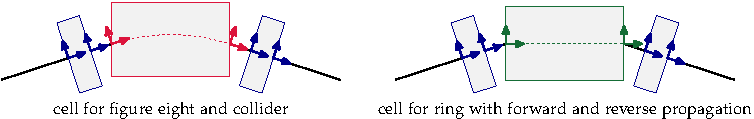
\includegraphics{Layouts/models-00}
  \caption{Basic cells for the three accelerator models.}
  \label{fig:basic.cells}
\end{figure}

\fref[c]{basic.cells} illustrates the two basic cells. We outline
the quadrupoles in blue, the rectangular bend in red, and the
``straight'' bend in green. The black lines indicate the drifts.
The cell with the rectangular bend does not require patching  because the reference frames of
adjacent elements lie on top of one another. The cell with the
``straight'' bend, however, requires patching t because the adjacent drifts have frames that
are rotated with repect to those of the ``straight'' bend.

\index{build_PSR@\ptc{build_PSR}!basic ring}
%
The basic ring (see the \ptc{build_PSR} example in \fref{DNA.subrtns}
on \pref{fig:DNA.subrtns}) has ten cells. It has 70~fibres, each pointing
to one of 70~elements. The ring with forward and reverse propagation has
140~fibres pointing to 140~elements.

The figure-eight and the collider each have 140~fibres pointing to
134~elements. In each of those models the upper and lower rings share
the elements at the start of one cell (long drift, quadrupole, short
drift) and the elements at the end of another cell (short drift,
quadrupole, long drift).

\begin{figure}[ht]
  \centering
  %\includegraphics[width=\textwidth]{illustrations/model-tutorial}
  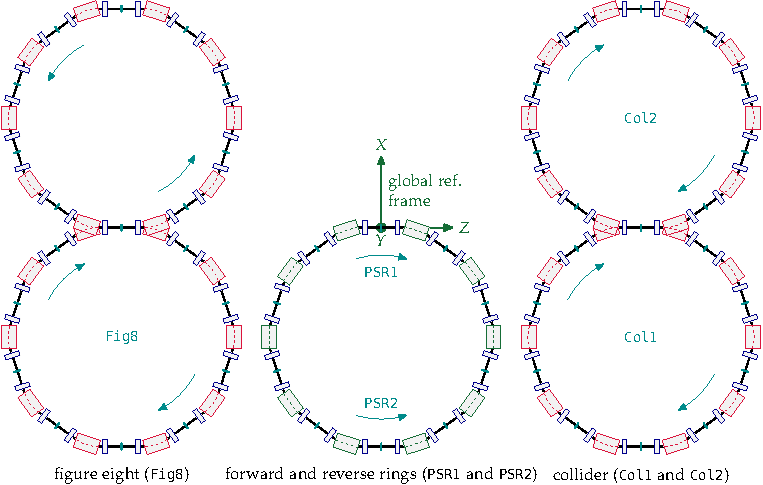
\includegraphics{Layouts/models-01}
  \caption{Accelerator models. Arrows indicate the direction of motion
           of particle beams in the constituent layouts.}
  \label{fig:accel.models}
\end{figure}

Our three tutorial examples are not real accelerators: They do not
have particle injectors or dumps; and two of the examples are not
physically possible, because some of their elements overlap in space.
The goal of these examples is to introduce the principal \PTC\ concepts
involved in modeling the geometry of an accelerator. After learning
these concepts, we can use \PTC\ to model complex real-world
accelerators.


\section{Geometry Tutorial Source File}
\label{sec:geom.tut}

\index{PTC!source file}
\index{source file!geometry tutorial}
\index{geometry!tutorial source file}
\index{ptc_geometry.f90@\ptc{ptc_geometry.f90}!geometry tutorial source file}
%
The example code in this chapter is from the \PTC\ geometry tutorial
source file, \ptc{ptc_geometry.f90}, which is given in
\Aref{geom.tutorial}. The line numbers of the code in the examples
refer to the line numbers of the code in that appendix.


\subsection{Initial Code}
\label{sec:init.code}

The initial code in the \ptc{ptc_geometry.f90} source file
includes type declarations and performs some initialization.

\setptclinenums{1}{5}
\begin{ptccode}[
  label={\ptctitle{\ptc{ptc_geometry.f90}\quad\small This program
                   describes the geometry of several \PTC\ lattices.}}
]
program ptc_geometry
use madx_ptc_module
use pointer_lattice
implicit none

logical(lp) :: doit
integer :: i, j, mf, pos, example
real(dp) :: b0
real(dp), dimension(3) :: a, d
real(dp), dimension(6) :: fix1, fix2, mis, x
type(real_8), dimension(6) :: y1, y2
type(layout), pointer :: L1, L2, L3, L4, L5, L6
type(layout), pointer :: PSR1, PSR2, Fig8, Col1, Col2
type(fibre), pointer :: p1, p2, p3, pf, b, f
type(internal_state) :: state

! some simple fitting objects for the fake collider complex
type(pol_block) :: qf(2), qd(2) 
type(normalform) :: n1, n2
type(damap) :: id
type(taylor) :: eq(4)
type(gmap) :: g
!-----------------------------------
!-----------------------------------
    interface
       subroutine build_PSR(PSR)
         use madx_ptc_module
         use pointer_lattice
         implicit none
         type(layout), target :: PSR
       end subroutine build_PSR
       subroutine build_PSR_minus(PSR)
         use madx_ptc_module
         use pointer_lattice
         implicit none
         type(layout), target :: PSR
       end subroutine build_PSR_minus
       subroutine build_Quad_for_Bend(PSR)
         use madx_ptc_module
         use pointer_lattice
         implicit none
         type(layout), target :: PSR
       end subroutine build_Quad_for_Bend
    end interface
!

call ptc_ini_no_append          \label{lin:init.layout}
\end{ptccode}

%\fxnote{What does \ptc{use_info = .true.} do?!?}

\index{PTC!universe}
\index{universe!PTC}
\index{MAD universe|see{PTC universe}}
\index{global variable!\ptc{m_u}}
\index{m_u@\ptc{m_u}!global variable}
\index{DNA database!\ptc{m_u} global variable}
\index{module!\ptc{madx_ptc_module}}
\index{madx_ptc_module@\ptc{madx_ptc_module}!module}
\index{linked list!\ptc{m_u} global variable}
%
\et{The module \ptc{madx_ptc_module}  defines the global variable}
\ptc{m_u}.\label{mad.univ}%
\sidenote{Think "\emph{M}\textsc{ad} \emph{U}niverse".}
This variable, which we shall use frequently, denotes a linked list
of layouts%
\sidenote{We use the linked-list aspect of \ptc{m_u} only briefly
in \STref{DNA.array}.}
that will \et{contain} our \DNA\ database \et{as well as the trackable layouts.} 

%The \ptc{gino}
%mentioned on \lref{gino} refers to a
%Windows$^\text{\textregistered}$-based graphical user
%interface developed for \PTC\ by \'Etienne Forest.
%Its use is not required.

\PTC\ uses the following type declarations for modeling accelerator
topologies:
\begin{itemize}
  \item \ptc{real(dp)} for double precision real numbers,
  \item \ptc{type(layout)} for \ptctyp{layout}s,
  \item \ptc{type(fibre)} for \ptctyp{fibre}s,
  \item \ptc{type(internal_state)} for setting the characteristic
         dynamics desired of your accelerator (see \TAref*{states}).
\end{itemize}
These data types will be discussed in this chapter.

\PTC\ uses the following type declarations for analyzing accelerator
properties \et{through the use of Taylor maps:}
\begin{itemize}
  \item \ptc{type(real_8)} for polymorphs,
  \item \ptc{type(pol_block)} for polymorphic blocks,
  \item \ptc{type(normalform)} for normal forms,
  \item \ptc{type(damap)} for a vector of Taylor maps
        (differential algebra maps),
  \item \ptc{type(taylor)} for single Taylor maps,
  \item \ptc{type(gmap)} for a vector of Taylor maps.
\end{itemize}
These latter data types will be described in \CTref*{polymorphs.knobs}.

\index{global variable!\ptc{lmax}}
\index{lmax@\ptc{lmax}!global variable}
\index{integration node!setting maximum length}
%
%The global variable \ptc{Lmax} defines the maximum length (here
%100~meters!) of an integration node. For more information about
%splitting elements into integration nodes,
%see \TCref*{symplectic.integ}.

%This initial code also, on \lref{init.layout}, initializes a layout;
%this must be done before starting \PTC's
%Gino$^\text{\textregistered}$-based graphical user interface for Windows.


\section{Subroutines}
\label{sec:geom.sub}

\index{DNA sequence!example source code}
\index{DNA database!example source code}
%
The end of the \ptc{ptc_geometry.f90} source file contains three
subroutines we use to create the \DNA\ sequences---non-trackable
layouts for our \DNA\ database. \fref[c]{DNA.subrtns} shows the
layouts that the three subroutines create. In subsequent sections
of this chapter, we describe how to use the layouts from this database,
or pieces of these layouts, to form the accelerator models of
\fref{accel.models}.

\begin{figure}[ht]
  \centering
  %\includegraphics[width=\linewidth]{illustrations/model-PSR}
  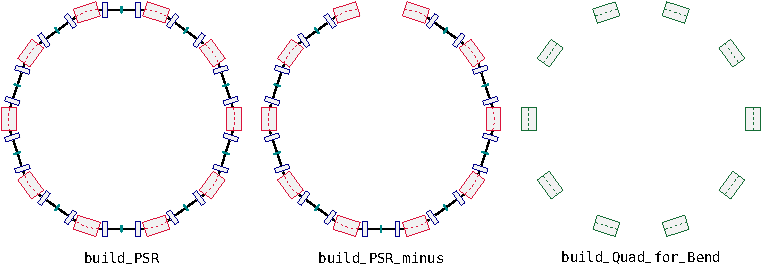
\includegraphics{Layouts/models-02}
  \caption{Subroutines for creating \DNA\ sequences.}
  \label{fig:DNA.subrtns}
\end{figure}


\subsection{build_PSR}
\label{sec:build.psr}

\index{build_PSR@\ptc{build_PSR}!example source code}
%
The subroutine \ptc{build_PSR} creates the basic ten-cell ring
lattice shown on the left in \fref{DNA.subrtns}.

\setptclinenums{532}{5}
\begin{ptccode}
subroutine  build_PSR(PSR)
use run_madx
use pointer_lattice
implicit none

type(layout), target :: PSR

real(dp) :: ang, brho, kd, kf, Larc
type(fibre) :: b, d1, d2, qd, qf
type(layout) :: cell
!-----------------------------------

call make_states(.false.)       \label{lin:bptc.psrstates}
exact_model = .true.
madlength = .false.             \label{lin:eptc.psrstates}

ang = (twopi * 36.d0 / 360.d0)
Larc = 2.54948d0
brho = 1.2d0 * (Larc / ang)
call set_mad(brho = brho, method = 2, step = 10) \label{lin:psr.setmad}
madkind2 = drift_kick_drift

kf =  2.72d0 / brho
kd = -1.92d0 / brho

d1 = drift("D1", 2.28646d0)     \label{lin:bptc.psrlatt}
d2 = drift("D2", 0.45d0)
qf = quadrupole("QF", 0.5d0, kf)
qd = quadrupole("QD", 0.5d0, kd)
b  = rbend("B", Larc, ang) \label{lin:psr.bend}
cell = d1 + qd + d2 + b + d2 + qf + d1 \label{lin:eptc.psrlatt}

PSR = 10 * cell
PSR = .ring.PSR                 \label{lin:psr.ring}

call survey(PSR)                \label{lin:psr.survey}
end subroutine build_PSR
\end{ptccode}

\index{internal states!example source code}
\index{state!internal}
\index{make_states@\ptc{make_states}!routine}
\index{routine!\ptc{make_states}}
\index{exact_model@\ptc{exact_model}!global parameter}
\index{global parameter!\ptc{exact_model}}
\index{madlength@\ptc{madlength}!flag}
\index{flag!\ptc{madlength}}
%
\glossary[ptccmds](make_states)%
  {make_states(<\textit{\normalfont{bool}}>)}%
  {This subtoutine sets internal-state variables associated
   with the particle type.
   In particular, use \ptc{call make_states(true)} for electrons,
   and \ptc{call make_states(false)} for protons.}
%
The \lref[s]{bptc.psrstates}--\lref*{eptc.psrstates} set important
internal state variables for tracking. In the call to
\ptc{make_states}, the boolean argument \ptc{.false.} means we are
modeling a proton lattice. Use \ptc{.true.} for electrons.%
\sidenote{For other particles, use the ratio of particle mass to
electron mass as the argument of \ptc{make_states}.}
To use the full ``square-root'' Hamiltonian, we set the global
parameter \ptc{exact_model} to \ptc{.true.} 
%
%The global variable
%\ptc{default}, of type \ptctyp{internal_state}, is here modified
%from its default value by adding the following two flags:
%\begin{itemize}
%  \item \ptc{nocavity}, which tells \PTC\ to ignore RF cavities;
%  \item \ptc{exactmis}, which tells \PTC\ to treat misalignments exactly.
%\end{itemize}
%(For more on internal-state variables, see \Aref{states}.)
Finally, we set the flag \ptc{madlength} to \ptc{.false.} This
means that \PTC\ will use the arc length, rather than the chord
length, to define the geometry of a rectangular bending magnet.
Use \ptc{.true.} to make \PTC\ use the chord length. \et{The line \ptc{madkind2 = drift_kick_drift} sets the explicit symplectic integrator to a drift-kick-drift split.}

\begin{marginfigure}\forcerectofloat
  %\includegraphics{illustrations/rbend}
  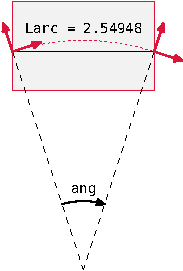
\includegraphics{Layouts/models-04}
  \caption{Geometry of the rectangular bend.}
  \label{fig:rect.bend}
\end{marginfigure}

%\fxnote{Need to say something about \ptc{madkind2}.}

\index{set_mad@\ptc{set_mad}!routine}
\index{routine!\ptc{set_mad}}
\index{integration nodes!specifying number of}
\index{energy!specifying}
%
\label{set.mad}
The call, in \lref{psr.setmad}, to \ptc{set_mad} defines (via
\ptc{brho}) the scale momentum $p_o$ for the fibres in the
layout returned by this subroutine. It also specifies the type
(\ptc{method = 2}) and number (\ptc{STEP = 10}) of integration steps
in the body of each element. We then define the five fibres needed
for our basic cell:
\begin{itemize}
  \item Fibres \ptc{d1} and \ptc{d2} denote the long and short drifts.
  \item Fibres \ptc{qf} and \ptc{qd} denote the focusing and defocusing
        quadrupoles.
  \item And fibre \ptc{b} denotes the rectangular bending magnet.
        Note that it is defined by its arc length and bend angle---here
        \ptc{Larc} and \ptc{ang}, respectively.
        See \fref{rect.bend}.
\end{itemize}
The symbols in quotes (\eg, \ptc{"QF"}) are the \emph{names} given
to these elements.%
\sidenote{Because a layout may have any number of these elements,
the names actually define \emph{classes} of elements.}
We may now define the variable \ptc{cell}, of type \ptctyp{layout}, as
the appropriate sequence of fibres. Finally, the layout \ptc{PSR}
returned by this subroutine is defined as 10 cells, and
\lref{psr.ring} modifies \ptc{PSR} to make it a ring, \ie, closed.

\index{survey@\ptc{survey}!routine}
\index{routine!\ptc{survey}}
%
At this point, \lref{psr.ring}, the elements of the \PSR\ lattice
are present, and in the correct sequence of fibres, in layout
\ptc{PSR}. But should we ask for the location of those elements,%
\sidenote{The way to ask this of \PTC\ will become clear later in
this chapter. See, for example, \pref{move.elem}---especially the
discussion of moving and rotating elements.}
we would discover that all of them have their entrance frames at
the global origin.  In other words, they are all stacked on top
of one another at the global origin.
%\linenumberfrequency{0}
%\begin{ptccode}[frame=none]
%  p => PSR%start
%  do i = 1, PSR%n
%    write(mf,'(a)') p%mag%name
%    write(mf,'(a,3(1x,f13.7))') "a:   ", p%chart%f%a
%  end do
%\end{ptccode}
The call to \ptc{survey} causes \PTC\ to loop through the fibres in
\ptc{PSR}, moving each element so that its entrance frame coincides
with the exit frame of the previous element. For the \PSR\ lattice,
the reference frames for the bends and quadrupoles line up exactly
with those of their adjacent drifts. As a consequence, this lattice
requires no patching. We have therefore finished building the
\PSR\ lattice in \PTC.



\newthought{Some readers will complain} that the set of
\lref[s]{bptc.psrlatt} through \lref*{eptc.psrlatt} violates the
philosophy of \PTC---and they have a point. This may seem subtle,
but we urge all other readers to invest the time required to
comprehend this point. Look, for example, at the definition of the
bend given in \lref{psr.bend}. After careful consideration of this
definition and what happens on the succeeding lines, the reader
should recognize that this definition actually serves a dual purpose.
On the one hand, the setting of arc length and bend angle define the
\emph{geometry} of the element. On the other hand, this line also
serves to define the \emph{physics} of this element. To verify this
claim, query \PTC\ for the magnetic field of this element:
\linenumberfrequency{0}
\begin{ptccode}[frame=none]
  write(6,'(a,f7.4)') "PSR B-field = ", b%mag%bn(1) * brho
\end{ptccode}
\linenumberfrequency{5}
will do the trick. You will learn that \PTC\ already knows the
magnetic field has a value of \SI{1.2}{T}! This information, of
course, requires a knowledge of not only the geometry, but also the
particle mass and energy. \emph{Here} is the apparent violation of
the \PTC\ philosophy, which aims to separate the geometric
description of beamline elements (location, reference frames, \etc)
from their physical content (magnetic field strength, \etc). The
resolution of this conflict lies in the fact that once we have
nailed down the geometry, we are then free to modify the lattice
with misalignments, changes to the magnetic field, and the like.

\et{
\newthought{Some readers, who fully understand the flexibility of PTC,  will most certainly object to \lref{psr.survey}! } 
Indeed the claim is, as the reader will discover soon, that magnets can be placed in any bizarre positions. Then what is the \ptc{survey} command doing?
Forest claimed that he could have chosen to be more ``Catholic than the Pope'' in which case the \ptc{survey} command would not exist.
Indeed one can place magnets ``manually'' and \PTC\ can then compute the necessary patches between them. This is the ``fundamentalist'' view of \PTC . With that philosophy, the survey command is useless.  


Indeed most lattices, or pieces of lattices, come from standard codes. In standard codes the survey command places the magnets using the assumption that no patches are needed between the elements. Therefore a simple sequence like the Bmad sequence \ptc{CELL: LINE=( D1M,SD1,QD,D2,SD2,B,D2,SD2,QF,D1)} already assumes a relative placement of the magnets.

 The reader must realize that the locution ``assumes no patches'' is completely code dependent. \PTC\ and Bmad use the geometry described in the  MAD8
manual from which a ``no patch'' lattice entails a certain relative placement. However, for lattices involving vertical bends, the result will differ from the code SAD of KEK. In the code SAD, the exit frame of a rotated bend will not be lined up with that of a vertically rotated bend in MAD8. Therefore the survey command of SAD will produce a different lattice from MAD, \PTC\ or Bmad. In MAD, the rotation that brings  a dipole off the mid-plane is undone at the exit. In SAD, it  is not so as SAD tries to ``parallel transport'' the frame of reference. 

It is important to realize, in the lens frame work, that the frame of references are really arbitrary. No one can say that SAD is better than MAD or vice versa. \PTC\ adopted the MAD convention simply because Forest collaborated initially with the MAD team. Actually Forest emphasizes this point by stating that he often has the urge to rotate the exit frame of reference of all magnets by some arbitrary angle just to prove this point. 

In reality, it is possible to link \PTC\ with a CAD program and generate an arbitrarily oriented sequence of magnets requiring patches. This is the power of \PTC\ that we try to explain here. 

Ultimately the survey command of \PTC\ has two minor purposes. First, from  purely internal point of view, it insures self-consistency. If a lattice has been patched, then the survey command, which tracks the positions of the lattice through should not ``move'' it. If it does then either patches are missing or badly computed. In any event \PTC\ is in a confused state. Secondly, most people will input into \PTC\ standard lattices and expect the standard survey command  of MAD to ``place'' the magnets in their (relative) correct place. If \PTC\ did not have a survey command, any standard user would scream for it!

But in summary, simply remember that \PTC\ can put the magnets in any arbitrary position and then track the beam. \PTC\ is ideally suited to be incorporated in a CAD program and produce ``instant'' tracking through a complex 3-d geometry.

}
\subsection{build_PSR_minus}

\index{build_PSR_minus@\ptc{build_PSR_minus}!example source code}
%
The subroutine \ptc{build_PSR_minus} defines the partial ring shown
in the center of \fref{DNA.subrtns}. It begins with a bend, a short
drift, a quadrupole, and a long drift; it continues with eight
\PSR\ cells; and it concludes with a long drift, a quadrupole, a short
drift, and a bend. Relative to the \PSR\ lattice, this partial ring is
missing a short drift, a quadrupole, two long drifts, a quadrupole,
and a short drift. The subroutine is a straightforward modification of
that for \ptc{build_PSR}.
%
\fxnote{Actually, this code sets \ptc{method=6} in the call to
\ptc{set_mad}. Should we change this, or comment on it?}

\linenumberfrequency{5}
\setptclinenums{572}{5}
\begin{ptccode}
subroutine  build_PSR_minus(PSR)
use madx_ptc_module
use pointer_lattice
implicit none

type(layout), target :: PSR

real(dp) :: ang, brho, kd, kf, Larc
type(fibre) :: b, d1, d2, qd, qf
type(layout) :: cell
!-----------------------------------

call make_states(.false.)
exact_model = .true.
madlength = .false.

ang = (twopi * 36.d0 / 360.d0)
Larc = 2.54948d0
brho = 1.2d0 * (Larc / ang)
call set_mad(brho = brho, method = 6, step = 10)
madkind2 = drift_kick_drift

kf =  2.72d0 / brho
kd = -1.92d0 / brho

d1 = drift("D1", 2.28646d0)
d2 = drift("D2", 0.45d0)
qf = quadrupole("QF", 0.5d0, kf)
qd = quadrupole("QD", 0.5d0, kd)
b  = rbend("B", Larc, ang)
cell = d1 + qd + d2 + b + d2 + qf + d1

PSR = b + d2 + qf + d1 + 8 * cell + d1 + qd + d2 + b
PSR = .ring.PSR

call survey(PSR)
end subroutine build_PSR_minus
\end{ptccode}


\subsection{build_Quad_for_Bend}

\index{build_Quad_for_Bend@\ptc{build_Quad_for_Bend}!example source code}
%
The subroutine \ptc{build_Quad_for_Bend} defines the layout shown
on the right in \fref{DNA.subrtns}. It has ten ``straight'' bends,
which have the same length as the rectangular bends in the
\PSR\ lattice. Because the entrance and exit frames of the ``straight''
bends are not rotated, we will need to insert patches everywhere.
These patches will describe both rotations and drifts between the
elements. In fact, because this layout contains no focusing elements,
its entries will be used only in other layouts.

\setptclinenums{612}{5}
\begin{ptccode}
subroutine  build_Quad_for_Bend(PSR)
use run_madx
use pointer_lattice
implicit none

type(layout),target :: PSR

real(dp) :: ang, ang2, brho, b1, Larc, Lq
type(fibre) :: b
!-----------------------------------

call make_states(.false.)
exact_model = .true.
madlength = .false.

ang = (twopi * 36.d0 / 360.d0)
Larc = 2.54948d0
brho = 1.2d0 * (Larc / ang)
call set_mad(brho = brho, method = 6, step = 10)
madkind2 = drift_kick_drift     \label{lin:qfb.same}

ang2 = ang / two                \label{lin:bptc.qfb.bend}
b1 = ang / Larc
Lq = Larc * sin(ang2) / ang2

b = quadrupole("B_QUAD", Lq, 0.d0);
call add(b, 1, 0, b1)           \label{lin:qfb.b1}
b%mag%permfringe = .true.       \label{lin:bptc.qfb.frng}
b%magp%permfringe = .true.
b%mag%p%bend_fringe = .true.
b%magp%p%bend_fringe = .true.   \label{lin:eptc.qfb.bend}

PSR = 10 * b
PSR = .ring.PSR

call survey(PSR)                \label{lin:qfb.survey}
end subroutine build_Quad_for_Bend
\end{ptccode}

Except for some changes in the type declarations, the code through
\lref{qfb.same} in this subroutine is identical to that in the
previous two subroutines. The ``straight'' bend is created in
\lref[s]{bptc.qfb.bend} through \lref*{eptc.qfb.bend}. We first
compute the length \ptc{Lq} as the chord length of the \PSR's
rectangular bend. To achieve the desired ``straight'' reference
frames, we define the ``straight'' bend as a zero-strength
quadrupole. Then, to make this a dipole, we set, in \lref{qfb.b1},
the normalized dipole strength of \ptc{b} to the computed value
\ptc{b1}. Finally, we set some flags to give this magnet the fringe
fields appropriate to a rectangular bend.

Query: After the call to \ptc{survey} in \lref{qfb.survey}, where
in the global frame are the magnets that this subroutine defines?%
\sidenote{They lie all in a straight line, one after the other,
starting at the global origin and extending to a point 10\,\ptc{Lq}
out along the $z$ axis. Making this layout look like the right-hand
layout of \fref{DNA.subrtns} will require more work.}


\section{Populating the \DNA\ Database}
\label{sec:pop.DNA}

\index{DNA database!populating}
\index{DNA sequence!populating DNA database}
\index{layout!non-trackable}
%
Using the subroutines described in the previous section, we shall
populate our \DNA\ database with six \DNA\ sequences (non-trackable
layouts): \ptc{L1}, \ptc{L2}, \ptc{L3}, \ptc{L4}, \ptc{L5}, and
\ptc{L6}. Note that we shall want each element in our three
accelerator models to appear once and only once in the \DNA-sequence
portion of the \DNA\ database. This uniqueness will reflect the
uniqueness of the individual beamline elements in our accelerators.

\index{layout!trackable}
%
Layouts \ptc{L1} and \ptc{L2} will provide the elements for the
concentric rings accelerator: trackable layouts \ptc{PSR1} and
\ptc{PSR2}. (See \fref{accel.models}.) Layouts \ptc{L3} and \ptc{L4}
will provide the elements for the figure-eight accelerator: trackable
layout \ptc{Fig8}. And layouts \ptc{L5} and \ptc{L6} will provide the
elements for the collider: trackable layouts \ptc{COL1} and \ptc{COL2}.
\tref[c]{DNA.dbase} summarizes the layouts we plan to create: six
\DNA\ sequences, or non-trackable layouts, and the five trackable layouts.

\begin{table}[t]
  \caption{DNA database for the \PTC\ geometry tutorial}
  \label{tbl:DNA.dbase}
  \begin{center}
    \begin{tabular}{ll} \toprule
  Non-trackable layouts & Trackable layouts \\ \midrule
  \ptc{L1}: 70 elements (\ptc{build_PSR}) & 
    \ptc{PSR1}: created from \ptc{L1} and \ptc{L2} \\
  \ptc{L2}: 10 elements (\ptc{build_Quad_for_Bend}) & 
    \ptc{PSR2}: created from \ptc{L1} and \ptc{L2} \\
  \ptc{L3}: 64 elements (\ptc{build_PSR_minus}) & 
    \ptc{Fig8}: created from \ptc{L3} and \ptc{L4} \\
  \ptc{L4}: 70 elements (\ptc{build_PSR}) & 
    \ptc{Col1}: created from \ptc{L6} \\
  \ptc{L5}: 64 elements (\ptc{build_PSR_minus}) & 
    \ptc{Col2}: created from \ptc{L5} and \ptc{L6} \\
  \ptc{L6}: 70 elements (\ptc{build_PSR}) & \\ \bottomrule
    \end{tabular}
  \end{center}
\end{table}

Query: As initially constructed (by \ptc{build_PSR}), layouts \ptc{L1},
\ptc{L4}, and \ptc{L6} are identical. So also are layouts \ptc{L3} and
\ptc{L5}. Why don't we avoid this duplication?%
\sidenote{Because we want to be able to modify---move, mispower,
\etc--- the individual elements. We do not want changes made to
\ptc{COL1}, for example, to appear in \ptc{Fig8}. \et{All the elements of the DNA are distinct magnets which must exist independently of each other.} }

\index{append_empty_layout@\ptc{append_empty_layout}!routine}
\index{routine!\ptc{append_empty_layout}}
\index{global variable!\ptc{m_u}}
\index{m_u@\ptc{m_u}!global variable}
%
The following four lines create the first \DNA\ sequence:
%
\setptclinenums{60}{5}
\begin{ptccode}
call append_empty_layout(m_u) ! DNA sequence 1
call set_up(m_u%end)
L1 => m_u%end
call build_PSR(L1); L1%name="L1";
\end{ptccode}
%
The call to \ptc{append_empty_layout} appends an empty layout to
the global linked list of layouts \ptc{m_u}. The layout pointer
\ptc{m_u\%end} points to this empty layout. The second line
initializes this new layout; and the third line makes \ptc{L1} point
to it. Finally, the call to \ptc{build_PSR} populates layout \ptc{L1}
with the 70 elements shown for the \PSR\ in \fref{DNA.subrtns}.

We repeat this process five times for layouts \ptc{L2}, \ptc{L3},
\ptc{L4}, \ptc{L5}, and \ptc{L6}. For \ptc{L2}, we call
\ptc{build_Quad_for_Bend}, which populates that layout with 10~elements
(the ``straight'' bends). For \ptc{L3}, we call \ptc{build_PSR_minus},
which populates that layout with 64 elements. And for \ptc{L4},
\ptc{L5}, and \ptc{L6}, we repeat the calls to \ptc{build_PSR} and
\ptc{build_PSR_minus}.
%
\setptclinenums{65}{5}
\begin{ptccode}
call append_empty_layout(m_u) ! DNA sequence 2
call set_up(m_u%end)
L2 => m_u%end
call  build_Quad_for_Bend(L2); L2%name="L2";

call append_empty_layout(m_u) ! DNA sequence 3
call set_up(m_u%end)
L3 => m_u%end
call build_PSR_minus(L3); L3%name="L3";

call append_empty_layout(m_u) ! DNA sequence 4
call set_up(m_u%end)
L4 => m_u%end
call build_PSR(L4); L4%name="L4";

call append_empty_layout(m_u) ! DNA sequence 5
call set_up(m_u%end)
L5 => m_u%end
call build_PSR_minus(L5); L5%name="L5";

call append_empty_layout(m_u) ! DNA sequence 6
call set_up(m_u%end)
L6 => m_u%end
call build_PSR(L6); L6%name="L6";
\end{ptccode}
%
We now have six \DNA\ sequences, or non-trackable layouts, in our
\DNA\ database. Moreover, each beamline element appears just once
in that database.

\index{doko!described}
\index{element!doko for multiple use}
%
The \PTC\ type \ptctyp{element} contains an object, \ptc{doko}
(from the Japanese word for ``where''), that enables \PTC\ to
keep track of which fibres point to a given beamline element.
This object \ptc{doko} allows \PTC\ to use a given element multiple
times in the database of trackable layouts. We shall see several
examples of this in the next section.



\section{Modeling Complex Accelerator Topologies}
\label{sec:model.topos}

%The next step is to create the trackable layouts.
%When we are done, we will set up the \DNA\ arrays.

\index{accelerator topology!complex}
\index{modeling!accelerator topologies}
\index{layout!trackable}
%
In the previous section, we created the layouts in the left-hand
column of \tref{DNA.dbase}. We now set about creating the
layouts (right-hand column of \tref{DNA.dbase}) for the three
accelerator models shown in \fref{accel.models}: the ring with
forward and reverse propagation, the figure-eight lattice, and
the collider. Complex accelerator topologies typically have a
one-to-many correspondence between some of the beamline elements
(stored in the \DNA\ sequences of the \DNA\ database) and the
fibres in the trackable layouts. By the end of this section, you
should understand how to set up such correspondences.

\et{
In \Sref{model.topo2s} and beyond, we will see an alternative way to store the \DNA\ and trackable layouts.
The \DNA\ will be stored in the  mad_universe \ptc{m_u} while all the trackable will be located in the universe \ptc{m_t}.
It will be possible to scan the universe  \ptc{m_u} with a single pointer. But, in the mean time, let us follow the older way of doing things: a single universe for \DNA\ and trackable layouts.
}

\subsection{Ring with Forward and Reverse Propagation}

\begin{marginfigure}[4\baselineskip] \forceversofloat
  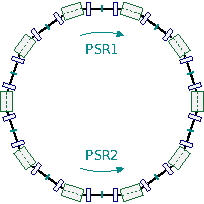
\includegraphics{Layouts/models-05}
  \caption{Ring with forward and reverse propagation.}
  \label{fig:fwd.rev.ring}
\end{marginfigure}

\index{accelerator topology!model of ring with forward and reverse propagation}
\index{ring with forward and reverse propagation!modeling}
\index{forward propagation!example}
\index{backward propagation!example}
%
Here we model an accelerator that carries a pair of
counter-propagating beams (\fref{fwd.rev.ring}, also middle
lattice in \fref{accel.models}). The two beams will propagate
through different layouts---\ptc{PRS1} for the forward-propagating
beam, and \ptc{PRS2} for the backward-propagating beam---but
the two trackable layouts must, of course, share the same ring
with the same beamline elements. They will just have different
directions of propagation and oppositely charged particles.

There is a further complication: this ring uses ``straight'' bends
instead of rectangular bends (see \fref{basic.cells}). In order to
place these elements in their proper locations, we will use the
lattice of layout \ptc{L1} as a guide, taking the ``straight''
bends from layout \ptc{L2}.%
\sidenote{The point of this complication is to illustrate some of
\PTC's geometry operations and the process of patching.
It should also, we hope, emphasize the \LEGO-block concepts of
\PTC\ (\cf\ \fref{LEGO.maps} and the associated discussion).}
The final result will be a pair of layouts, \ptc{PSR1} and
\ptc{PSR2}, each of which refer to fibres in two different
\DNA\ sequences, \ptc{L1} and \ptc{L2}.

\index{append_empty_layout@\ptc{append_empty_layout}!routine}
\index{routine!\ptc{append_empty_layout}}
%
We begin by calling \ptc{append_empty_layout} on \ptc{m_u} and then
setting the layout pointer \ptc{PSR1} to point to this new layout:
%
\setptclinenums{94}{2}
\begin{ptccode}
!== PSR1 : forward ring  (layout 7)
call append_empty_layout(m_u)
PSR1 => m_u%end
\end{ptccode}
%
We shall populate this layout with a linked list of fibres taken
appropriately from layouts \ptc{L1} and \ptc{L2}. Two fibre
pointers \ptc{p1} and \ptc{p2} will step through these two layouts,
and a third fibre pointer, \ptc{f}, will keep track of our location
in \ptc{PSR1}. Elements taken from \ptc{L1} have the correct
geometric relations, but the ``straight'' bends taken from \ptc{L2}
will have to be moved to their correct locations.

\setptclinenums{98}{5}
\begin{ptccode}
p1 => L1%start
p2 => L2%start
do i = 1, L1%n
  if(p1%mag%name == "B") then
    ! read bends from L2
    call append_point(PSR1, p2)    \label{lin:psr1.append.L2}
    f => PSR1%end                  \label{lin:psr1.bgeom}
    d = p1%chart%f%o - f%chart%f%o \label{lin:psr1.comp.d}
    call translate(f, d)           \label{lin:psr1.trans.d}
    call compute_entrance_angle(f%chart%f%mid, p1%chart%f%mid, a) \label{lin:psr1.comp.a}
    call rotate(f, f%chart%f%o, a, basis = f%chart%f%mid) \label{lin:psr1.egeom}
    p2 => p2%next                  \label{lin:psr1.advance.p2}
  else
    call append_point(PSR1, p1)    \label{lin:psr1.append.L1}
  end if
  p1 => p1%next                    \label{lin:psr1.advance.p1}
end do ! elements in PSR1 now in correct locations
\end{ptccode}

\index{append_point@\ptc{append_point}!routine}
\index{routine!\ptc{append_point}}
%
In the above block of code, we point \ptc{p1} and \ptc{p2}
respectively to the starts of \DNA\ sequences \ptc{L1} and \ptc{L2}.
The \ptc{do} loop over the \ptc{L1\%n} fibres in \ptc{L1} appends
to \ptc{PSR1} the desired fibres from \ptc{L1} or \ptc{L2}---bends
from \ptc{L2}, everything else from \ptc{L1}:
\begin{itemize}
  \item If \ptc{p1} points to a bend, then in \lref{psr1.append.L2}
    we append the current fibre of \ptc{L2} to \ptc{PSR1}. This, of
    course, will always be a ``straight'' bend---a \ptc{B_QUAD}.
    Later, in \lref{psr1.advance.p2}, we advance \ptc{p2} to the next
    fibre in \ptc{L2}.
  \item If \ptc{p1} does \emph{not} point to a bend, then in
    \lref{psr1.append.L1} we append the current fibre of \ptc{L1}
    to \ptc{PSR1}.
  \item In either case, we advance, in \lref{psr1.advance.p1},
    \ptc{p1} to the next fibre in \ptc{L1}.
\end{itemize}

\index{translate@\ptc{translate}!routine}
\index{routine!\ptc{translate}}
\index{compute_entrance_angle@\ptc{compute_entrance_angle}!routine}
\index{routine!\ptc{compute_entrance_angle}}
\index{rotate@\ptc{rotate}!routine}
\index{routine!\ptc{rotate}}
\index{global frame!used to compute local reference frame}
%
After we append a ``straight'' bend to \ptc{PSR1}, we must do
some extra work to place it in the correct location. Since we
want a given ``straight'' bend to have the same location and
orientation as the corresponding rectangular bend, we simply
compute and perform the required translations and rotations.
This happens in \lref[s]{psr1.bgeom} through \lref*{psr1.egeom}:
\label{move.elem}
\begin{enumerate}
  \item Point \ptc{f} to the fibre most recently appended to
    \ptc{PSR1}.
  \item Compute, in \lref{psr1.comp.d}, the vector \ptc{d}
    from the center of the newly appended ``straight'' bend
    (\ptc{f\%chart\%f\%o})%
    \sidenote{Read \ptc{f\%chart\%f\%o} as
    ``\ptc{f}-chart-frame-center''.}
    to the center of the corresponding
    rectangular bend in \ptc{L1} (\ptc{p1\%chart\%f\%o}).
  \item Translate the newly appended fibre (\lref{psr1.trans.d}).
  \item Compute, in \lref{psr1.comp.a}, the rotation \ptc{a}
    from the frame attached to the middle of the newly appended
    ``straight'' bend (\ptc{f\%chart\%f\%mid}) to the frame
    attached to the middle of the corresponding rectangular bend
    in \ptc{L1} (\ptc{p1\%chart\%f\%mid}).%
    \sidenote{Because rotations do not commute, their order is
    important. \PTC\ performs co\"ordinate rotations in the order
    $x$-axis, $-y$-axis, $z$-axis.}
%    Note that \ptc{a} denotes a real three-vector (see
%    \TPref{sec:init.code} \lref{decl.ad}).
  \item Rotate the newly appended fibre about its center
    (\ptc{f\%chart\%f\%o}) by angles \ptc{a}, which are given
    with respect to the frame attached to the middle of that
    element (\ptc{f\%chart\%f\%mid}).
\end{enumerate}

\index{find_patch@\ptc{find_patch}!routine}
\index{routine!\ptc{find_patch}}
\index{patch!inserting}
\index{patching!find_patch@\ptc{find_patch} routine}
%
When the above \ptc{do} loop terminates, the beamline elements of
\ptc{PSR1} are all in their correct locations. However (recall the
discussion concerning \fref{basic.cells}) the ``straight'' bends
of \ptc{PSR1} all require patching. This happens in the following
block of code:
%
\setptclinenums{116}{5}
\begin{ptccode}
f => PSR1%start
do i = 1, PSR1%n
  if(f%mag%name == "B_QUAD") then
    call find_patch(f%previous, f, next = .true.)
    call find_patch(f, f%next, next = .false.)
  end if
  f => f%next
end do ! PSR1 now patched
\end{ptccode}
%
Within the \ptc{do} loop over all elements in \ptc{PSR1}, we apply
the patches required between each \ptc{B_QUAD} (or ``straight'' bend)
and its preceding and trailing elements. No other elements require
patching. \et{If a CAD program was linked to \PTC , which would be of great use, then the need for patching would always be there as soon as a magnet is moved. A CAD program would use \PTC\ in its purest and intended form: magnets have no preferential placement. }

Finally, in the following three lines of code, we give layout \ptc{PSR1}
a formal name, and we ensure that it forms a closed topological ring,
so that particles can circulate. Note that the second two lines must
\emph{both} be executed to make the layout \ptc{PSR1} form a closed ring.
The call to \ptc{ring_L} in \lref{psr1.ringL} sets some pointers inside
the layout \ptc{PSR1} that connect the end of \ptc{PSR1} to the start,
and vice versa.
%
\setptclinenums{125}{5}
\begin{ptccode}
PSR1%name = "PSR 1"
PSR1%closed = .true.
call ring_L(PSR1, .true.) ! make it a ring topologically \label{lin:psr1.ringL}
\end{ptccode}

Query: At this point, where in the global frame are the magnets,
the ``straight'' bends, of layout \ptc{L2}?%
\sidenote{\label{sn:geom.L2}%
The geometry operations performed on the bend \ptctyp{fibre}s of
\ptc{PSR1} applied, ultimately, to the \ptctyp{element}s in \ptc{L2}.
Hence those elements are now oriented as in the right-hand layout of
\fref{DNA.subrtns}, with the global origin centered between the
adjacent ends of the top two magnets.}

To construct layout \ptc{PSR2} for the backward-propagating beam,
we follow essentially the same steps as for \ptc{PSR1}. (See the
next block of code.) There are three significant differences:
(i) In this case, all the elements are already in their proper
physical locations,${}^\text{\ref{sn:geom.L2}}$ so here we may
omit the geometric computations
and operations performed during the construction of \ptc{PSR1}.
(ii) Because of the backwards propagation, we initialize the
pointers \ptc{p1} and \ptc{p2} respectively to the \emph{ends} of
layouts \ptc{L1} and \ptc{L2}; and we advance those pointers not
to the next but to the \emph{previous} fibres in their respective
layouts. (See \lref[s]{psr2.prev2} and \lref*{psr2.prev1}.)
(iii) We must add the information that the beam described by this
layout traverses its elements in the reverse direction
(\lref{psr2.opp.dir}) and has particles with negative charge
(\lref{psr2.opp.chg}).%
\sidenote{Both direction and charge are properties of fibres,
and both default to +1.}
%
\setptclinenums{129}{5}
\begin{ptccode}
!== PSR2 : backward ring (layout 8)
call append_empty_layout(m_u)
PSR2 => m_u%end

p1 => L1%end
p2 => L2%end
do i = 1, L1%n
  if(p1%mag%name == "B") then
    call append_point(PSR2, p2)
    p2 => p2%previous            \label{lin:psr2.prev2}
  else
    call append_point(PSR2, p1)
  end if
  f => PSR2%end
  f%dir = -1                     \label{lin:psr2.opp.dir}
  f%charge = -1                  \label{lin:psr2.opp.chg}
  p1 => p1%previous              \label{lin:psr2.prev1}
end do

f => PSR2%start
do i = 1, PSR2%n
  if(f%mag%name == "B_QUAD") then
    call find_patch(f%previous, f, next = .true.)
    call find_patch(f, f%next, next = .false.)
  end if
  f => f%next
end do

PSR2%name = "PSR 2"
PSR2%closed = .true.
call ring_L(PSR2, .true.) ! make it a ring topologically
\end{ptccode}

Trackable layouts \ptc{PSR1} and \ptc{PSR2} are now complete.
Both contain 70 fibres pointing to the same set of 70 elements
in \DNA\ sequences \ptc{L1} and \ptc{L2}.


\subsection{Figure-Eight}

\index{accelerator topology!model of figure eight}
\index{figure-eight accelerator!modeling}
%
Here we model a figure-eight lattice---the left-hand lattice in
\fref{accel.models}. It carries a single beam clockwise (forward)
around the lower ring, then counter-clockwise (backward) around
the upper ring. The two rings share several elements in one
straight section. See \fref{accel.fig8}. The single trackable
layout \ptc{Fig8} we shall construct from \DNA\ sequences \ptc{L3}
and \ptc{L4} (see \tref{DNA.dbase}). For the lower ring, we use
the full ten-cell \PSR\ lattice in layout \ptc{L4}. For the upper
ring, we use all of layout \ptc{L3} (\ptc{PRS_minus}), and we
re-use six of the fibres in layout \ptc{L4}. In addition, so that
this layout does not overlap our previous layouts, \ptc{PSR1} and
\ptc{PSR2}, we shall place it \SI{40}{m} distant in the negative~$z$
direction.

\begin{figure}[ht]
  \centering
  %\includegraphics{illustrations/model-fig8}
  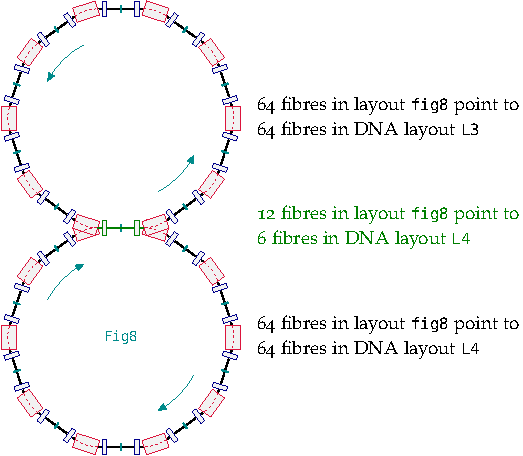
\includegraphics{Layouts/models-03}
  \caption{\ptc{Fig8} fibres pointing to elements in \ptc{L3}
           and \ptc{L4}.}
  \label{fig:accel.fig8}
\end{figure}

The construction of layout \ptc{Fig8} takes place in the following
six blocks of code. We describe each in detail.

\index{global frame!positioning first element in trackable layout}
\index{rotate@\ptc{rotate}!routine}
\index{routine!\ptc{rotate}}
%
In this first block of code, we translate layout \ptc{L4} a
distance \SI{40}{m} in the negative~$z$ direction
(\lref[s]{fig8.btr4}--\lref*{fig8.etr4}).
We then (\lref[s]{fig8.brot}--\lref*{fig8.erot}) rotate layout
\ptc{L3} \ang{180} about the entrance of its first element
(\ptc{L3\%start\%chart\%f\%a}). This rotates the gap in \ptc{L3}
down to the bottom. Now note that the bend to the right of this
gap (after the rotation) belongs to the last fibre in \ptc{L3}.
To finish placing \ptc{L3} in the correct location, we want the
\emph{end} of its last bend to coincide with the entrance of the
first bend in the lower ring, \ptc{L4}. See \fref{ring.match}.
We therefore point, in \lref{fig8.mvp1}, the fibre pointer
\ptc{p1} to the first bend (\ptc{"B"}) in \ptc{L4}; compute, in
\lref{fig8.comp.d}, the vector \ptc{d} from the exit of the last
bend in \ptc{L3} (\ptc{L3\%end\%chart\%f\%b}) to the entrance of
the first bend in \ptc{L4} (\ptc{p1\%chart\%f\%a}); and then
translate, in \lref{fig8.tr3}, layout \ptc{L3} by vector \ptc{d}.
%
\setptclinenums{162}{5}
\begin{ptccode}
!== Fig8 : figure-eight lattice (layout 9)
d = zero                                \label{lin:fig8.btr4}
d(3) = -40.d0
call translate(L4, d)                   \label{lin:fig8.etr4}
a = zero                                \label{lin:fig8.brot}
a(2) = pi
call rotate(L3, L3%start%chart%f%a, a)  \label{lin:fig8.erot}
call move_to(L4, p1, "B", pos)          \label{lin:fig8.mvp1}
d = p1%chart%f%a - L3%end%chart%f%b     \label{lin:fig8.comp.d}
call translate(L3, d)                   \label{lin:fig8.tr3}
\end{ptccode}
%
At this point, the beamline elements for the figure-eight lattice
are all correctly located and oriented.



\index{append_empty_layout@\ptc{append_empty_layout}!routine}
\index{routine!\ptc{append_empty_layout}}
%
In the next block of code, we first call \ptc{append_empty_layout}
on \ptc{m_u} and set the layout pointer \ptc{Fig8} to point to this
new layout. Then, in \lref[s]{fig8.bapp.L4}--\lref*{fig8.eapp.L4},
we append in order all the fibres of \ptc{L4} to \ptc{Fig8}.
%
\setptclinenums{173}{5}
\begin{ptccode}
call append_empty_layout(m_u)
Fig8 => m_u%end
p1 => L4%start                 \label{lin:fig8.bapp.L4}
do i = 1, L4%n
  call append_point(Fig8, p1)
  p1 => p1%next                \label{lin:fig8.p1next}
end do                         \label{lin:fig8.eapp.L4}
\end{ptccode}
%
\begin{marginfigure}[-29\baselineskip]\forceversofloat
  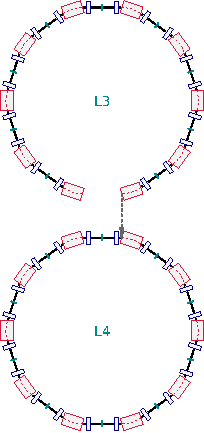
\includegraphics{Layouts/models-06}
  \caption{Matching \ptc{L3} to \ptc{L4}.}
  \label{fig:ring.match}
\end{marginfigure}
We now have the complete lower ring.

\index{append_point@\ptc{append_point}!routine}
\index{routine!\ptc{append_point}}
\index{doko!described}
%
In the next block of code, we start to include the upper ring by
appending to \ptc{Fig8} the first three fibres of the lower ring.
These three new fibres in \ptc{Fig8} will, of course, point to the
same physical elements as do the first three fibres in \ptc{Fig8}:
a long drift, a defocusing quadrupole, and a short drift. During
the calls to \ptc{append_point}, \PTC\ will add this information
to the \ptc{doko}s of the corresponding elements in \ptc{L4}. As a
consequence, each of those three elements in \DNA\ sequence \ptc{L4}
knows that it is pointed to by two different fibres in trackable
layout \ptc{Fig8}.%
\sidenote{Each of those elements already knows it belongs to a
fibre in layout \ptc{L4}.}



Note that we need not initialize the pointer \ptc{p1} to \ptc{L4\%start}: the last execution, in \lref{fig8.p1next}, of \ptc{p1 => p1\%next} returns \ptc{p1} to the beginning of the layout.
%
\setptclinenums{181}{5}
\begin{ptccode}
call append_point(Fig8, p1)
p1 => p1%next
call append_point(Fig8, p1)
p1 => p1%next
call append_point(Fig8, p1)
\end{ptccode}

In the next block of code, we append the fibres of layout \ptc{L3}
to \ptc{Fig8}. Since our beam traverses \ptc{L3} in the reverse
direction, we initialize the fibre pointer \ptc{p1} to \ptc{L3\%end}
(\lref{fig8.p1.set1}), and we advance that pointer to the
\emph{previous} fibre (\lref{fig8.prev1}). During this process,
we take care of two other tasks: We tell \PTC\ that these elements
are traversed in the reverse direction (\lref{fig8.opp.dir}); and,
if the element is a bend, we reverse the sign of the magnetic field
(\lref{fig8.revb}). The particle charge remains the same (default
value +1).
%
\setptclinenums{169}{5}
\begin{ptccode}
p1 => L3%end                   \label{lin:fig8.p1.set1}
do i = 1, L3%n
  call append_point(Fig8, p1)
  Fig8%end%dir = -1            \label{lin:fig8.opp.dir}
  if(p1%mag%name == "B") p1%mag%bn(1) = -p1%mag%bn(1) \label{lin:fig8.revb}
  p1 => p1%previous            \label{lin:fig8.prev1}
end do
\end{ptccode}

\index{doko!described}
%
To complete the upper ring, and hence our trackable layout
\ptc{Fig8}, three fibres remain to be appended: the last three
fibres of the lower ring, \ptc{L4}. This is accomplished in the
next block of code. First, in \lref{fig8.p1.set2}, we point
\ptc{p1} to the fibre containing the short drift near the end of
layout \ptc{L4}. We then append to \ptc{Fig8} that fibre and the
next two. During the calls to \ptc{append_point}, \PTC\ will add
the appropriate information to the \ptc{doko}s of the corresponding
elements.
%
\setptclinenums{195}{5}
\begin{ptccode}
p1 => L4%end%previous%previous  \label{lin:fig8.p1.set2}
call append_point(Fig8, p1)
p1 => p1%next
call append_point(Fig8, p1)
p1 => p1%next
call append_point(Fig8, p1)
\end{ptccode}

\index{check_need_patch@\ptc{check_need_patch}!routine}
\index{routine!\ptc{check_need_patch}}
\index{find_patch@\ptc{find_patch}!routine}
\index{routine!\ptc{find_patch}}
\index{patch!inserting}
\index{patch!checking whether needed}
\index{patching!\ptc{find_patch} routine}
\index{patching!\ptc{check_need_patch} routine}
%
Finally, in the last block of code for \ptc{Fig8}, we give our new
layout a formal name (\ptc{"Figure-Eight"}), ensure that it is
topologically closed, and apply any necessary patches. The call to
\ptc{check_need_patch}, \lref{fig8.chk.patch}, returns the integer
\ptc{pos} equal to zero if no patch is needed. A non-zero value
indicates the type of patch required. By using \ptc{check_need_patch},
we can apply patches only where necessary. Our figure-eight lattice
requires patching because some of the constituent elements are
traversed in the reverse direction. In particular, there are adjacent
fibres \ptc{f} which have opposite values of \ptc{f\%dir}. This
happens between the short drift at end of the common straight section
and the first bend of the upper ring; and also between the last bend
of the upper ring and the subsequent short drift.
%
\setptclinenums{202}{5}
\begin{ptccode}
Fig8%name = "Figure-Eight"
Fig8%closed = .true.
call ring_L(Fig8, .true.) ! make it topologically closed

p1 => Fig8%start
do i = 1, Fig8%n
  call check_need_patch(p1, p1%next, 1.d-10, pos)  \label{lin:fig8.chk.patch}
  if(pos /= 0) call find_patch(p1, p1%next, next = .false.)
  p1 => p1%next
end do
\end{ptccode}

Trackable layout \ptc{Fig8} is now complete. It has 140~fibres
pointing to 134~elements in \DNA\ sequences \ptc{L4} and \ptc{L3}.
Twelve of the fibres in \ptc{Fig8} point to the six elements (four
drifts and two quadrupoles at the top of \ptc{L4}) which are common
to the upper and lower rings. See \fref{accel.fig8}.

\et{There is an interesting anecdote concerning the \PTC\ model of the LHC by Forest and Schmidt. Forest connected the injection line of LHC2 to LHC2 itself. This required a tiny angle due to the kicker at the end of the injection line. However since the injection line had been designed  using forward propagators and the LHC2 is made of backwards propagators, patching also requires a rotation of 180 degrees. Forest was asked, during his presentation, if he had not forgotten to put that rotation. His answer was simply: ``Let us see if \PTC\ has put it.''  Indeed examination of the flat file showed that  \PTC\ had correctly identified the need for a patch. In MADX, the user must on his own, through unreliable brain power, realize that a rotation of 180 degrees is needed to bring the outward horizontal direction of one beam line into what appears to be an inward $x$-direction: look at the common area of the Figure-Eight or the collider.  }


\subsection{Collider}


\index{accelerator topology!model of collider}
\index{collider!modeling}
%
Here we model a collider---\fref{col1.col2}, also the right-hand
lattice in \fref{accel.models}---which has clockwise propagating
beams in each of its two rings. This model comprises two layouts,
\ptc{Col1} and \ptc{Col2}, which we shall construct from
\DNA\ sequences \ptc{L5} and \ptc{L6} (see \tref{DNA.dbase}). For
the lower ring, we use the full ten-cell \PSR\ lattice in layout
\ptc{L6}. For the upper ring, we use all of layout \ptc{L5}
(\ptc{PRS_minus}), and we re-use six of the fibres in layout
\ptc{L6}.%
\sidenote{Yes, this sounds much like the description for layout
\ptc{Fig8}. Be sure to note the \emph{differences}.}
In addition, so that this layout does not overlap our previous
layouts, \ptc{PSR1}, \ptc{PSR2}, and \ptc{Fig8}, we shall place
it \SI{40}{m} distant in the positive~$z$ direction.

The construction of layouts \ptc{Col1} and \ptc{Col2} takes place
in the following four blocks of code. We describe each in detail.

\begin{marginfigure}
  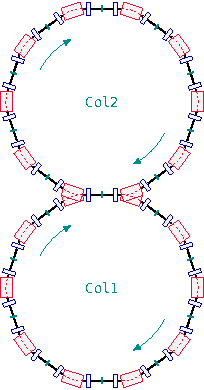
\includegraphics{Layouts/models-07}
  \caption{Collider.}
  \label{fig:col1.col2}
\end{marginfigure}

In this first block of code, we place all the beamline elements of
layouts \ptc{Col1} and \ptc{Col2} in their correct locations: We
translate layout \ptc{L6} a distance \SI{40}{m} in the positive~$z$
direction. We then rotate layout \ptc{L5} \ang{180} about the
entrance of its first element (\ptc{L5\%start\%chart\%f\%a}). This
rotates the gap in \ptc{L5} down to the bottom. To finish placing
\ptc{L5} in the correct location, we want the \emph{end} of its
last bend to coincide with the entrance of the first bend in the
lower ring, \ptc{L6}. We therefore point layout pointer \ptc{p1}
to the first bend (\ptc{"B"}) in \ptc{L6}; compute the vector
\ptc{d} from the exit of the last bend in \ptc{L5}
(\ptc{L5\%end\%chart\%f\%b}) to the entrance of the first bend in
\ptc{L6} (\ptc{p1\%chart\%f\%a}); and then translate layout \ptc{L5}
by that vector \ptc{d}.
%
\setptclinenums{213}{5}
\begin{ptccode}
!== Col1 : lower collider ring (layout 10)
!== Col2 : upper collider ring (layout 11)
d = zero
d(3) = 40.d0
call translate(L6, d)
a = zero
a(2) = pi
call rotate(L5, L5%start%chart%f%a, a)
call move_to(L6, p1, "B", pos)
d = p1%chart%f%a - L5%end%chart%f%b
call translate(L5, d)
\end{ptccode}

\index{append_empty_layout@\ptc{append_empty_layout}!routine}
\index{routine!\ptc{append_empty_layout}}
\index{append_point@\ptc{append_point}!routine}
\index{routine!\ptc{append_point}}
%
In the next block of code, we construct layout \ptc{Col1}: We
call \ptc{append_empty_layout} on \ptc{m_u} and set the layout
pointer \ptc{Col1} to point to this new layout. Then we append
in order all the fibres of \ptc{L6} to \ptc{Col1}. Finally, we
give our new layout a formal name (\ptc{"Collider 1"}) and ensure
that it is topologically closed. This layout does not require
patching.
%
\setptclinenums{225}{5}
\begin{ptccode}
call append_empty_layout(m_u)
Col1 => m_u%end
p1 => L6%start
do i = 1, L6%n
  call append_point(Col1, p1)
  p1 => p1%next
end do

Col1%name = "Collider 1"
Col1%closed = .true.
call ring_L(Col1, .true.) ! make it a ring topologically
\end{ptccode}

In the next block of code, we construct layout \ptc{Col2}: We call
\ptc{append_empty_layout} again on \ptc{m_u}, set the layout
pointer \ptc{Col2} to point to this new layout, and then locate,
in \lref{col2.next.next}, the first short drift in layout \ptc{L6}.
To populate \ptc{Col2}, we now, in
\lref[s]{col2.bapp.str}--\lref*{col2.eapp.str}, march backwards
appending the six elements in the straight section at the top of
layout \ptc{L6} (short drift, defocusing quadrupole, two long drifts,
focusing quadrupole, and short drift). While doing this, we inform
\PTC, in \lref{col2.opp.dir}, that this layout traverses those
elements in the opposite direction. Finally, in
\lref[s]{col2.bapp.L5}--\lref*{col2.eapp.L5}, we append in order all
the fibres of \ptc{L5} to \ptc{Col2}.
%
\setptclinenums{237}{5}
\begin{ptccode}
call append_empty_layout(m_u)
Col2 => m_u%end
p1 => L6%start%next%next    \label{lin:col2.next.next}
do i = 1, 6                 \label{lin:col2.bapp.str}
  call append_point(Col2, p1)
  Col2%end%dir = -1         \label{lin:col2.opp.dir}
  p1 => p1%previous
end do                      \label{lin:col2.eapp.str}
p1 => L5%start              \label{lin:col2.bapp.L5}
do i = 1, L5%n
  call append_point(Col2, p1)
  p1 => p1%next
end do                      \label{lin:col2.eapp.L5}
\end{ptccode}

\index{check_need_patch@\ptc{check_need_patch}!routine}
\index{routine!\ptc{check_need_patch}}
\index{find_patch@\ptc{find_patch}!routine}
\index{routine!\ptc{find_patch}}
\index{patch!inserting}
\index{patch!checking whether needed}
\index{patching!\ptc{find_patch} routine}
\index{patching!\ptc{check_need_patch} routine}
%
In this last block of code for \ptc{Col2}, we give our new layout a
formal name (\ptc{"Collider 2"}), ensure that it is topologically
closed, and apply any necessary patches. This layout requires patches
only where \ptctyp{fibre}\ptc{\%dir} switches sign. As in our earlier
layout \ptc{Fig8}, this happens at the two ends of the common straight
section, where they join the bends of the upper ring.
%
\setptclinenums{251}{5}
\begin{ptccode}
Col2%name = "Collider 2"
Col2%closed = .true.
call ring_L(Col2, .true.) ! make it a ring topologically

p1 => Col2%start
do i = 1, Col2%n
  call check_need_patch(p1, p1%next, 1.d-10, pos)
  if(pos /= 0) call find_patch(p1, p1%next, next = .false.)
  p1 => p1%next
end do
\end{ptccode}

The trackable layouts \ptc{Col1} and \ptc{Col2} are now complete.
They have 140 fibres pointing to 134 elements in \DNA\ sequences
\ptc{L6} and \ptc{L5}. Twelve of the fibres in \ptc{Col1} and
\ptc{Col2} point to the six elements which are common to the upper
and lower rings.


\section{DNA Arrays}
\label{sec:DNA.array}

\index{DNA array!described}
\index{layout!trackable}
\index{DNA database!storing trackable layouts}
\index{allocate@\ptc{allocate}!routine}
\index{routine!\ptc{allocate}}
%
The following code constitutes a bit of housekeeping. We have created a set of six layouts---\ptc{L1}--\ptc{L6}---that form the core of our \DNA\ database. What we do here is tell each of the trackable layouts we have created---\ptc{PSR1}, \ptc{PSR2}, \ptc{Fig8}, \ptc{Col1}, and \ptc{Col2}---which \DNA\ sequences they use. This information is stored in the array \ptc{DNA} that is part of the data held in each \PTC\ \ptctyp{layout}.

In \lref{dna.L1} we record in \ptc{PSR1} the fact that \DNA\ sequence \ptc{L1} is used by \ptc{PSR1}. Then \lref{dna.L2} records the fact that \ptc{PSR1} also uses \DNA\ sequence \ptc{L2}. Note that this latter line makes use of the linked-list character of our \DNA\ database. (Recall, see \pref{mad.univ}, that \ptc{m_u} is a linked list of layouts.) Since \ptc{PSR1\%DNA(1)\%L} already points to \ptc{L1} (see \lref{dna.L1}), and since \ptc{L2} is the next layout in the \DNA\ database, then \ptc{PSR1\%DNA(1)\%L\%next} points to \ptc{L2}. (In this very simple case you could, of course, replace \lref[s]{dna.bdo}--\lref*{dna.edo} with the single statement \ptc{PSR1\%DNA(2)\%L => L2}.) The remaining lines in this block of code populate the \DNA\ arrays for the other trackable layouts.
%
\setptclinenums{267}{5}
\begin{ptccode}
allocate(PSR1%DNA(2))
PSR1%DNA(1)%L => L1                           \label{lin:dna.L1}
do i = 2, 2                                   \label{lin:dna.bdo}
  PSR1%DNA(i)%L => PSR1%DNA(i-1)%L%next ! L2  \label{lin:dna.L2}
end do                                        \label{lin:dna.edo}

allocate(PSR2%DNA(2))
PSR2%DNA(1)%L => L1
do i = 2, 2
  PSR2%DNA(i)%L => PSR2%DNA(i-1)%L%next ! L2
end do

allocate(Fig8%DNA(2))
Fig8%DNA(1)%L => L3
do i = 2, 2
  Fig8%DNA(i)%L => Fig8%DNA(i-1)%L%next ! L4
end do

allocate(Col1%DNA(2))
Col1%DNA(1)%L => L5
do i = 2, 2
  Col1%DNA(i)%L => Col1%DNA(i-1)%L%next ! L6
end do

allocate(Col2%DNA(2))
Col2%DNA(1)%L => L5
do i = 2, 2
  Col2%DNA(i)%L => Col2%DNA(i-1)%L%next ! L6
end do
\end{ptccode}

\section{Modeling Complex Accelerator Topologies with two ``MAD universes''}
\label{sec:model.topo2s}

The program \ptc{new_ptc_geometry.f90} is very similar to the program
we just examined. \DNA\ or databased layouts are created in the same
manner; trackable layouts are also created identically as far as the
process is concerned. The main difference is in the storage of these
objects. The database layouts are stored in the database universe
\ptc{m_u}. The trackable layout are stored in the trackable universe
\ptc{m_t}. With this setup we could dispense with the \DNA\ pointers
described in the previous section, although they might still be very
useful.

To explain this process, we created a new program
\ptc{new_ptc_geometry.f90} that contains purposely some empty lines so
that the line numbers align perfectly with \ptc{ptc_geometry.f90}. In
doing so, we facilitate comparison. The \DNA\ pointers are left in the
code since they are used in the fitting example.t

As we will see, the database universe \ptc{m_u} contains all the
necessary information and can be scanned as a single linked list
irrespective of the number of layouts it happens to contain.

\setptclinenums{1}{5}
\begin{ptccode}[
  label={\ptctitle{\ptc{new_ptc_geometry.f90}\quad\small This program
                   describes the geometry of several \PTC\ lattices using two ``MAD universes.''}}
]
program new_ptc_geometry
use madx_ptc_module
use pointer_lattice
implicit none

logical(lp) :: doit
integer :: i, j, mf, pos, example,poss
real(dp) :: b0
real(dp), dimension(3) :: a, d
real(dp), dimension(6) :: fix1, fix2, mis, x
type(real_8), dimension(6) :: y1, y2
type(layout), pointer :: L1, L2, L3, L4, L5, L6
type(layout), pointer :: PSR1, PSR2, Fig8, Col1, Col2
type(fibre), pointer :: p1, p2, b, f
type(internal_state) :: state
type(fibre_appearance), pointer :: next_doko
! some simple fitting objects for the fake collider complex
type(pol_block) :: qf(2), qd(2)
type(normalform) :: n1, n2
type(damap) :: id
type(taylor) :: eq(4)
type(gmap) :: g
!-----------------------------------
!-----------------------------------
    interface
       subroutine build_PSR(PSR)
         use madx_ptc_module
         use pointer_lattice
         implicit none
         type(layout), target :: PSR
       end subroutine build_PSR
       subroutine build_Quad_for_Bend_New(PSR)
         use madx_ptc_module
         use pointer_lattice
         implicit none
         type(layout), target :: PSR
       end subroutine build_Quad_for_Bend_New
       subroutine build_PSR_minus(PSR)
         use madx_ptc_module
         use pointer_lattice
         implicit none
         type(layout), target :: PSR
       end subroutine build_PSR_minus
    end interface

call ptc_ini_no_append \label{lin:init.layout2}
write(6,*) "Do you want to read an accelerator complex ? yes=1 "  \label{lin:read:uni1}
read(5,*) poss
if(poss==1) then
 call read_universe_database(m_u,'m_u.txt',arpent=my_false)
 call read_universe_pointed(M_u,M_t,'m_t.txt')
 call create_dna(M_u,m_t)
 goto 999
end if  \label{lin:read:uni2}
\end{ptccode}

The first major difference is the possibility of reading the full accelerator complex if it has been produced previously and printed out. 
The commands are found between \lref[s]{read:uni1} through \lref*{read:uni2}. 

All the layouts of the \DNA\ are loaded in the database universe \ptc{m_u} just as before. The major difference is that the trackable layouts are then created into the universe \ptc{m_t} rather than being appended to \ptc{m_u}..

 
{\scriptsize
\setptclinenums{94}{5}
\begin{ptccode}
!== PSR1 : forward ring  (layout 7)                       !== PSR1 : forward ring  (layout 1 of m_t)   \label{lin:dif:1}
call append_empty_layout(m_u)                             call append_empty_layout(m_t) \label{lin:dif:2}
PSR1 => m_u%end                                           PSR1 => m_t%end    \label{lin:dif:3}

p1 => L1%start                                                      
p2 => L2%start                                                      
do i = 1, L1%n                                                      
  if(p1%mag%name == "B") then                                       
    ! read bends from L2                                            
    call append_point(PSR1, p2)                                     
\end{ptccode}
}

This trivial difference is shown on \lref[s]{dif:2} and \lref*{dif:3}. The left hand side shows the original code where the first trackable layout \ptc{PSR1}  is appended at the end the universe \ptc{m_u}; therefore all trackable layouts will follow the database layouts.  On the right hand side, extracted from the program \ptc{new_ptc_geometry.f90}, the first  trackable \ptc{PSR1} is put in the universe \ptc{m_t}. The creation of the other trackable layouts follows the same pattern as \ptc{PSR1}.

With these two universes, the location of trackable and database layouts is unambiguous. Irrespective of their order of creation, all \DNA\ will be sequentially located in \ptc{m_u} and all trackable will be in \ptc{m_t}.

 
\section{Tying a Universe}
\label{sec:model.tie}

As before we can certainly construct the \DNA\ pointers. That still works. However because all the \DNA\ layouts  are in the same universe, it is useful to be able to scan that entire structure as one long link list of fibres. This is explore at the end of the program \ptc{new_ptc_geometry.f90}:

 
{ 
\setptclinenums{524}{5}
\begin{ptccode}
call kanalnummer(mf,"doko.txt")
call TIE_MAD_UNIVERSE(m_u)    \label{lin:tie:uni}
p1=>m_u%start%start
do i=1,m_u%nf  \label{lin:tie:do}
 write(mf,'(i4,1x,a16)') i,p1%mag%name
 next_doko=>p1%mag%doko
  do while(associated(next_doko))
   write(mf,'(a120)') next_doko%parent_fibre%parent_layout%name  \label{lin:lay:nam}
   p2=>next_doko%parent_fibre
   next_doko=>next_doko%next  \label{lin:lay:namn}
 enddo
 p1=>p1%n
end do
close(mf)

call ptc_end(graphics_maybe=2,flat_file=.true.)  \label{lin:ptc:end}
                                  
\end{ptccode}
}

The above piece of code does not do much beside illustrating the structure  of \PTC . First of all, at \lref{tie:uni}, the universe \ptc{\m_u} is ``tied,'' that is to say that a link list connects all the fibres of this universe. The pointers are \ptc{fibre\%p} and \ptc{fibre\%n} for the previous and next fibre respectively. These pointers are nullified if the universe is not tied. They should not be confused with the more important pointers \ptc{fibre\%previous} and \ptc{fibre\%next}  which are the links within a layout and are a quintessential part of \PTC .

The do-loop starting at \lref{tie:do}, scans the entire universe and locates all the occurrences of each magnet. Conversely one could scan a given trackable and check if the magnet is shared. This type of access to the magnets, fibres and layouts can be used in fitting routines to identify where a magnet is.

The result of this loop is printed in file \ptc{doko.txt}. Here is a little bit of that file:

{ 
\setptclinenums{1}{5}
\begin{ptccode}
     .
     .
     .
  66 D2              
PSR 1                                                                                                                   
PSR 2                                                                                                                   
  67 B           \label{lin:b:nil}     
  68 D2             
PSR 1                                                                                                                   
PSR 2                                                                                                                   
  69 QF         \label{lin:qf:psr}      
PSR 1                                                                                                                   
PSR 2                                                                                                                   
  70 D1              
PSR 1                                                                                                                   
PSR 2                                                                                                                   
  71 B_QUAD      \label{lin:b:q}         
PSR 1                                                                                                                   
PSR 2                                                                                                                   
  72 B_QUAD          
PSR 1                                                                                                                   
PSR 2                                                                                                                   
     .
     .
     .

 146 QD           \label{lin:qd:8}        
Figure-Eight                                                                                                            
Figure-Eight                                                                                                            
 147 D2              
Figure-Eight                                                                                                            
Figure-Eight                                                                                                            
 148 B               
Figure-Eight                                                                                                            
 149 D2              
Figure-Eight                                                                                                            
     .
     .
     .
\end{ptccode}
}


We first notice \lref{qf:psr}: it tells us that the quadrupole \ptc{QF} belongs to two objects:  \ptc{PSR1} and \ptc{PSR2}. Thus we are dealing most likely with a collider or some pretzel structure. In a huge object like the LHC, many magnets of the IR (interaction region) are shared between \ptc{LHC1} and \ptc{LHC2}.

On line \lref{qd:8} we see the ``opposite'' case: the same magnet appears twice in the beam line: this is the case of the common section of a ``figure 8'' lattice or a ``dog bone'' structure. This type of situation also appears in recirculators. 

Now we come to ``forensic'' evidence of our weird construction. \ptc{PSR1} and \ptc{PSR2} make a fake ``pretzel'', i.e., the same ring traversed in opposite direction. On  page \pageref{lin:psr1.append.L2} we explained how  the \DNA\ lattice \ptc{L1} creates the database for this pretzel. However, to show the power of patching, we replaced the normal dipole \ptc{B} (of \lref{b:nil}) by the straight elements of layout \ptc{L2}, namely the ten quadrupoles \ptc{B_QUAD}.

For convenience in the creation of this object, the original elements \ptc{B}, which are elements of \ptc{L1},  are never used in the final trackable lattices of \ptc{m_t}. Therefore there are no layouts using \ptc{B} as they fail to appear after \lref{b:nil}.  The database \ptc{m_u} contains magnets which seem to been in storage in the hangar of our imaginary laboratory. We could have avoided this state of affair, but this was the simpler thing to do. It would be a nice exercise in \PTC\ programming to rewrite \ptc{new_ptc_geometry.f90} to avoid these useless skeletons. 

\section{Avoidance of the cloning problem}
\label{sec:model.clone}


 \PTC\ is set up to avoid the ``cloning problem.'' This is best illustrated by an anecdote concerning the LHC lattice(s). Forest and Schmidt created a realistic model of the LHC based on the complex CERN database. This database contains ``assemblies'' and bending magnets which are in the same cryostat. These were realized in \PTC\ using the girder and siamese constructs which we will later described.

Forest and Schmidt put the same misalignment errors in the \PTC\ model as well as the standard representation of MADX, CERN's code. They then asked a co-worker to correct the orbit of LHC1 and LHC2. The values of the correctors were passed to the realistic \PTC\ model and \PTC\ plotted the orbit of LHC1 and LHC2.  The results were good in LHC1 but horrible in LHC2.

Question to the reader: assuming that both the \PTC\ model and MADX model are bug free, how can that be? The answer is cloning. Neither the defunct MAD9, the code that was supposed to end\footnote{It did end all attempts at using ``more advanced'' concepts. The decision was taken at CERN to take a minimalist approach to MADX: first MAD8 and make sure that by hook and crook MADX can do at least two rings.} all codes, nor MADX of CERN, nor SAD of KEK, is fundamentally capable of producing a \emph{faithful} representation of collider without ``hacking'' or ``bricolage'' as the French say.

In MADX, all the IR elements are cloned. Even more distasteful, the kickers of the IR regions are represented by RBENDs whose entrance and exit angles, normally a geometric number, depends on the trajectory obviously different in each ring. The error of our colleague was to use a shared kicker to correct the orbit. The orbit was first corrected in LHC2 and then in LHC1; the shared corrector was repowered for LHC1 with a value that simply messed up the trajectory of LHC2.  Since the rings of LHC1 and LHC2 are made of independent clones, the trajectories looked fine. However in \PTC\ only a single value could be entered because there is, \emph{ as in the real world}, a single magnet. Standard codes are like twin brothers  dating the same girl: as long as you keep all the bookkeeping straight, the perverse joke can go on. Eventually, the girl  may discover the truth. This is what happened with this MADX example. 


Both the codes \ptc{ptc_geometry.f90} and \ptc{new_ptc_geometry.f90} display a simple fitting algorithm using \TPSA . Cloning errors are impossible in \PTC .
The reader can look at the codes and see how all of this  works. It uses a simple ``\TPSA\'' inversion. More important for the present discussion is the assignment of knobs to be used in the fitting. The assignments of free knobs is done as follows:


\begin{ptccode}
qf(1) = 0
qf(1)%name = "qf"
qf(1)%ibn(2) = 1
qf(2) = 0
qf(2)%name = "qf"
qf(2)%ibn(2) = 3
qd(1) = 0
qd(1)%name = "qd"
qd(1)%ibn(2) = 2
qd(2) = 0
qd(2)%name = "qd"
qd(2)%ibn(2) = 4
Col1%dna(1)%L = qf(1)
Col1%dna(1)%L = qd(1)
CoL1%dna(2)%L = qf(2)
CoL1%dna(2)%L = qd(2)
\end{ptccode}

Since we attempt to fit simultaneously the tunes of \ptc{Col1} and \ptc{Col2} we need four free parameters or knobs. The first member of the \DNA\ of \ptc{Col1} is \ptc{L5}. These contains the elements of  \ptc{Col1} which are only in \ptc{Col1}. The second member of the \DNA\ is \ptc{L6} which is all of \ptc{Col2} including the elements it shares with \ptc{Col1}. 

The arrays \ptc{qf} and \ptc{qd} contains information about the \TPSA\ parameters which must appear in the map. The assignment \ptc{Col1\%dna(1)\%L = qf(1)} tells the code to scan the layout   \ptc{Col1\%dna(1)\%L} for any element that has the name \ptc{``qf'''} and make the quadrupole component the $1^{st}$ \TPSA\ parameter. It is imperative to realize that the \DNA\ contains no clones unless the user erroneously created an ``old fashioned '' lattice. Therefore there cannot be a double assignment  to any of the four quadrupoles.

Finally, it is worth pointing out that in a more realistic lattice with one interaction region, there would probably be a minimum of three \DNA\ layouts: the interaction region or intersection and the two pieces of \ptc{Col1} and \ptc{Col2} that contain magnets proper to themselves.  These things depends entirely on the designer and can be changed later once a quasi-final design is obtained. 

\section{The flat files}
\label{sec:model.flat}

A flat file is a description of the full lattice including girders and
siamese. In the case of a standard lattice, without girders and
siamese, \PTC\ can simply give the initial location in space and a
sequential list of all its elements.  The code \PTC, in that case,
behaves like any standard code. Fibres and elements (magnets), are in
one to one correspondence and can be confused. The relative positions
of the magnets can be computed using the \ptc{survey} command. The
absolute position can be computed either by giving an initial input to
the \ptc{survey} command or by moving the entire layout using a
rotation and/or a translation.

Additionally a standard lattice can have patches. The statements of
the previous paragraph apply \emph{in toto}. Although this is a novel
aspect of \PTC\ it is hardly revolutionary and still assumes that
magnets and fibres are interchangeable. For example, \PTC\ uses the
MAD8 convention for the survey. SAD, the KEK code, treats vertical
magnets differently as far as frame of references are
concerned. Therefore the survey command of SAD may produce a different
lattice than that of MAD8 or \PTC\ even on a standard lattice without
patches. In \PTC\ the translation between the two codes is handled by
an additional patch at the vertical bends that ensures that \PTC\ is
really modeling a SAD lattice.


The real power of \PTC\ is to be found in the modeling of colliders,
dogbones, figure eight and other strange contraptions where magnets
are visited more than once from different angles or, as in a collider,
belong to different lattices.  We have shown with the simple examples
of \ptc{ptc_geometry.f90} or, equivalently, with
\ptc{new_ptc_geometry.f90} how \PTC\ can create these complex
topologies.

Once these systems are created, either purely by \PTC\, or through the
intermediate use of a code like Bmad or with a CAD program, can one
save them and re-use them? The answer is yes if the creation mechanism
is based on the database universe \ptc{m_u} and trackable universe
\ptc{m_t} as described in \ptc{new_ptc_geometry.f90}. Would it be
possible to print and store the lattices created in
\ptc{ptc_geometry.f90}? Of course, since the physics is identical, the
answer must be ``yes.'' However Forest does not support this
option. One could theoretically translate the single universe
representation of \ptc{ptc_geometry.f90} into the double universe of
\ptc{new_ptc_geometry.f90} and print the accelerator complex. However
we simply advice the user of \PTC\ to use the double universe from the
very start as the code Bmad does when it constructs a complex topology
and sends it to \PTC .

\subsection{Printing the database universe}
%\label{sec:m_u.flat}

The file containing the database universe, \ptc{m_u.txt} in our
example, is made of two basic parts. First the \DNA\ layouts are
listed sequentially. In the example of this chapter, these are
\ptc{L1}, \ptc{L2}, \ptc{L3}, \ptc{L4}, \ptc{L5} and \ptc{L6}. Finally
the siamese magnets, which are magnets closely joined to each other,
are listed. And finally the girders are listed. Girders are assemblies
on which magnets and siamese can be attached. This permits \PTC\ to
have various level of misalignment errors in a lattice.
 
\setptclinenums{1}{5} 
\begin{ptccode}
L1                                                                                                                      
           2  highest fringe   \label{lin:mu:quad}
  1.000000000000000E+038  Maximum Length for Orbit 
 T T ALWAYS_EXACTMIS,ALWAYS_EXACT_PATCHING  \label{lin:mu:mis}
          10          10  SECTOR_NMUL_MAX,SECTOR_NMUL  \label{lin:mu:sect}
  $$$$$$$$$$$$$$$$$ START OF LAYOUT $$$$$$$$$$$$$$$$$
  $$$$$$$$$$$$$$$$$ INITIAL CHART $$$$$$$$$$$$$$$$$
  0.000000000000000E+000  0.000000000000000E+000  0.000000000000000E+000
   1.00000000000000       0.000000000000000E+000  0.000000000000000E+000
  0.000000000000000E+000   1.00000000000000       0.000000000000000E+000
  0.000000000000000E+000  0.000000000000000E+000   1.00000000000000     
  0.000000000000000E+000  0.000000000000000E+000   2.28646000000000     
   1.00000000000000       0.000000000000000E+000  0.000000000000000E+000
  0.000000000000000E+000   1.00000000000000       0.000000000000000E+000
  0.000000000000000E+000  0.000000000000000E+000   1.00000000000000     
  $$$$$$$$$$$$$$$$$ END OF INITIAL CHART $$$$$$$$$$$$$$$$$   \label{lin:mu:chart}
 &ELENAME
 ELE0%KIND    =          31,
 ELE0%NAME_VORNAME    = 'D1                      ' '                        ' ,
\end{ptccode}

\setptclinenums{1957}{5}
\begin{ptccode}
     .
     .
     .
L2 
     .
     .
     .
\end{ptccode}
\setptclinenums{7828}{5}
\begin{ptccode}
L6
     .
     .
     .
 &ELENAME
 ELE0%NAME_VORNAME='alldone','alldone', 
 /
           2  siamese in the universe \label{lin:mu:sia}
  0.000000000000000E+000  0.000000000000000E+000  0.000000000000000E+000  
  0.000000000000000E+000  0.000000000000000E+000   1.76354000000000        
           6           4         282 B                       
           5          64         278
           0           0           0
  0.000000000000000E+000  0.628318530717960       0.000000000000000E+000  \label{lin:sia:rot}
  0.774937120865398       0.000000000000000E+000  0.621471219233463            \label{lin:sia:tra}
           6          67         345 B                        \label{lin:sia:1}
           5           1         215                            \label{lin:sia:2}
           0           0           0
           1  girders in the universe 
  0.000000000000000E+000  0.000000000000000E+000   40.0000000000000      \label{lin:gir:f}
   1.00000000000000       0.000000000000000E+000  0.000000000000000E+000
  0.000000000000000E+000   1.00000000000000       0.000000000000000E+000
  0.000000000000000E+000  0.000000000000000E+000   1.00000000000000     
  0.000000000000000E+000  0.000000000000000E+000   40.0000000000000     
   1.00000000000000       0.000000000000000E+000  0.000000000000000E+000
  0.000000000000000E+000   1.00000000000000       0.000000000000000E+000
  0.000000000000000E+000  0.000000000000000E+000   1.00000000000000     
           6           1         279 D1      \label{lin:gir:m}                  
           6           2         280
           6           3         281
           6           4         282     \label{lin:gir:s11} 
           5          64         278    \label{lin:gir:s12} 
           5           1         215     \label{lin:gir:s22} 
           6          67         345    \label{lin:gir:s21}       
           5           8         222
           6          68         346
           6          69         347
           6          70         348
           0           0           0
\end{ptccode}

The first few lines contain global information; usually it is not advisable to have these parameters  changed unless you know what you are doing. Although they are listed in connection with \DNA\ layout \ptc{L1}, they should be common to your entire simulation. At \lref{mu:quad}, this parameter indicates that the highest hard edge  fringe field is of order $n=2$, i.e., a quadrupole. For example, if it is set to $n=3$,  the hard edge sextupoles are also computed if fringes are demanded by the user. 

At \lref{mu:mis} the code is instructed to compute the patches and misalignments exactly. Again, in particular with the patches, one must be careful in changing these parameters.

At \lref{mu:sect}, \PTC\ is instructed to solve Maxwell's equation to order $h^{10}$ in the sector bends where $h$ is the ideal curvature of the sector bend. This is only done for ``exact'' sector bends. 

The initial chart, which positions this layout, is actually not used in the \DNA\ layouts. 

The next part is the printing of the fibres. It is best to look at the code to have an idea. This code is found in \PTC 's \ptc{Sp_keywords.f90} in the subroutine \ptc{print_new_flat}:

\setptclinenums{1}{5} 
\begin{ptccode}
do i=1,ring%n
  call el_el0(f%mag,my_true,mf)   \label{lin:el:1}
  call fib_fib0(f,my_true,mf)    \label{lin:fib:1}
  CALL MC_MC0(f%MAG%P,my_true,mf)     \label{lin:mc:1}
  CALL print_ElementLIST(f%mag,MY_TRUE,mf)    \label{lin:list:1}
  if(f%patch%patch/=0) call patch_patch0(f%patch,my_true,mf)    \label{lin:patch:1}
  if(f%mag%mis) call CHART_CHART0(f%chart,my_true,mf)     \label{lin:chart:1}
 write(mf,*) " $$$$$$$$$$$$$$$$$ END OF FIBRE $$$$$$$$$$$$$$$$$"
 f=>f%next    
enddo
\end{ptccode}


First on \lref{el:1} data common to all magnets are printed in the Fortran name list \ptc{EL0}.  This includes the kind (an integer in \PTC ), the total length and the element name. It also includes quantities that strictly speaking are not common to all magnets but that are nevertheless in all magnets as  pointers, grounded if unused. For example the multipole arrays \ptc{an},  \ptc{bn}, the voltage, etc\ldots


On \lref{el:1} properties of the fibre are printed. Some of these properties truly do not belong here since this is a database layout. In fact, in a program better written that \PTC , the database would contain only magnets and no fibres. Unfortunately \PTC\ was written by a novice and suffers from logical defects. The reader will have to accept that the \DNA\ contains layouts. On the other hand, these have the advantage of being trackable: sometimes useful.

 On \lref{mc:1}, \PTC\ prints the information of the so-called \ptc{magnet_chart}. A lot of this information has to do with the geometry of the magnet: curved or straight. It contains also the edge angles of the bends and various flags for the fringe fields. The quantity \ptc{permfringe} has recently been turned into an integer to incorporate some fringe fields used by the code SAD of KEK. The method of integration, the number of steps and the highest multipole are also part of the information contained in the \ptc{magnet_chart}. When using a symplectic integrator, the number of integration steps is kept to a minimum and is an integral part of the model. It is not advisable to change the integration method ``on the fly.''

  On \lref{list:1}, \PTC\ prints information specific to that particular element. For many simple elements, it prints nothing! For example, in the case of a cavity, it will print the various harmonics of the cavity amongst other things. 

On \lref{patch:1}, \PTC\ will print patch information. \emph{Warning: this should not happen in a \DNA\ layout; but since this routine is used for traditional lattices, it is a possibility of the code.} 

On \lref{chart:1} a routine is called which prints misalignments of the magnet. Misalignments are truly a property of the magnet, not the fibre.  If a magnet is misaligned in one ring, then it is misaligned in all the rings and beam lines in which it belongs. Therefore \PTC\ considers misalignments to be part of the \DNA , defective \DNA\ to be sure, but \DNA\ nevertheless. 
 
The entire thing is repeated for all the fibres of the layout. Then layout are printed sequentially. In this example, there are six layouts described by more than  7800 lines of data. 

At \lref{mu:sia} of the database flat file \ptc{m_u.txt}, we finally arrive at the siamese and the girders. This is the first instance where \PTC\ must truly record a linked list.  The database universe is scanned for siamese groups and they are counted: here we have two siamese. It is easy to localize a group because the frame of reference of the siamese is attached to a single magnet of the group. 

For example, at \lref{sia:1}, the first magnet of the group is written down in the flat file:  it belongs to the sixth layout and it is the $67^{th}$ magnet. It is located in position 345 in the database universe \ptc{m_u}. The next magnet is in the fifth layout and at position 1.  Siamese are supposed to be closely linked like co-joined twins so can they really belong to different layouts? The answer is a resounding yes! For example in the LHC, for which there is a \PTC\ model made by Forest and Schmidt, the main bending magnets of LHC1 and LHC2 are siamese. They are in the same cryostat jacket. 

The position of the siamese is given with respect to the first magnet: this relative information is given at \lref[s]{sia:rot} and  \lref*{sia:tra}: a rotation and translation with respect to that first magnet at position 345 of the database universe.


The girders are described in a similar manner. The big difference is that the girder's center is located in space not with relative co\"ordinates attached to a member of the girder, but relative to the  frame of reference at  \lref{gir:f}. This frame of reference is attached (in a purely computer sense) to a magnet, \lref{gir:m}, as a pointer. 

The reader will notice that the two siamese defined at this example are members of a single girder, actually  only one girder is defined here. It would be possible to have a piece of a siamese on a girder and the other pieces elsewhere. However this would violate the philosophy of the siamese and girders. Think of the siamese as Wall Street criminals all chained together. Think of the girder as the bus taking them to incarceration. Although it would be nice to have them on separate buses since this would provide instant and severe punishment in case of accident, but we are sad to say, we do not live in the $18^{th}$ century when quartering was in practice. So we must  transport them on the same bus. The same is true with our magnets: misalignments of magnets within a siamese should be smaller than misalignments of siamese on girders, and finally girders can be badly misaligned, finally the center of mass of a layouts can be grossly unknown. 

Now, just as a example of the complexity of a system, the \DNA\ file for the LHC complex produced by Forest and Schmidt\sidenote{This files are available to the reader and are particularly interesting to run with Forest's Windows$^\text{\textregistered}$ graphical interface.} contains 4899 siamese and 2252 girders! The entire \DNA\ file contains 941039 ascii lines of which 874825 are the actual \DNA . The actual file of  trackables contains 68925 lines. This is the file we will now describe.  The size of this file is problem-dependent and therefore could contain more systems based in the same \DNA .

\subsection{Printing the trackable universe}
%\label{sec:m_u.flat}

First of all it is important to realize that one can create as many trackable was one needs. Trackable layout are mathematical  functions from a given position in the lattice to another one. For example we can have a trackable which includes an injection line and a piece of the ring in which it injects. Then we can have the full ring. These   two trackable will have magnets in common: one should never forget that change in one trackable is carried over all trackable layouts. Now we describe the 


\setptclinenums{1}{5} 
\begin{ptccode}
           5           6  trackable and DNA Layouts \label{lin:mt:1}
PSR 1           											\label{lin:mt:psr1}                                                                                                       
          70  Number elements in pointed layout                                       \label{lin:mt:first}   
  $$$$$$$$$$$$$$$$$ INITIAL CHART $$$$$$$$$$$$$$$$$  \label{lin:mt:chart1}   
  0.000000000000000E+000  0.000000000000000E+000  0.000000000000000E+000
   1.00000000000000       0.000000000000000E+000  0.000000000000000E+000
  0.000000000000000E+000   1.00000000000000       0.000000000000000E+000
  0.000000000000000E+000  0.000000000000000E+000   1.00000000000000     
  0.000000000000000E+000  0.000000000000000E+000   2.28646000000000     
   1.00000000000000       0.000000000000000E+000  0.000000000000000E+000
  0.000000000000000E+000   1.00000000000000       0.000000000000000E+000
  0.000000000000000E+000  0.000000000000000E+000   1.00000000000000     
  $$$$$$$$$$$$$$$$$ END OF INITIAL CHART $$$$$$$$$$$$$$$$$ \label{lin:mt:chart2}   
    1        1  0 D1                              1             \label{lin:mt:firstf}            
 &FIBRENAME
 FIB0%GAMMA0I_GAMBET_MASS_AG  =  0.540705256786713     ,  0.413152271219778     ,  0.938272013000000     ,   1.79284735000000     ,
 FIB0%CHARGE  =   1.00000000000000     ,
 FIB0%DIR     =           1,
 FIB0%PATCH   =           0
 /
    1        2  0 QD                              2  \label{lin:mt:2}    
    1        3  0 D2                              3  \label{lin:mt:3} 
    2        1  3 B_QUAD                          4   \label{lin:mt:4}                 
 &FIBRENAME
 FIB0%GAMMA0I_GAMBET_MASS_AG  =  0.540705256786713     ,  0.413152271219778     ,  0.938272013000000     ,   1.79284735000000     ,
 FIB0%CHARGE  =   1.00000000000000     ,
 FIB0%DIR     =           1,
 FIB0%PATCH   =           3
 /
 &PATCHNAME
 PATCH0%A_X1    =           1,
 PATCH0%A_X2    =           1,
 PATCH0%B_X1    =           1,
 PATCH0%B_X2    =           1,
 PATCH0%A_D     =  5.279424210553350E-017,  0.000000000000000E+000, -1.715388910777646E-017,
 PATCH0%B_D     = -3.424203176105467E-016,  0.000000000000000E+000, -8.490659797005278E-016,
 PATCH0%A_ANG   =  0.000000000000000E+000,  0.314159265358979     ,  0.000000000000000E+000,  \label{lin:rot:b}    
 PATCH0%B_ANG   =  0.000000000000000E+000,  0.314159265358979     ,  0.000000000000000E+000,  \label{lin:rot:e}    
 PATCH0%A_T     =  0.000000000000000E+000,
 PATCH0%B_T     =  0.000000000000000E+000,
 PATCH0%ENERGY  =      0,
 PATCH0%TIME    =      0
 /
\end{ptccode}

The first line, \lref{mt:1},  is  global to the entire file. It indicates the total number of database and trackable layouts. This facilitates the setting of the \DNA\ arrays, namely \ptc{LAYOUT\%DNA{:}\%L}. As we said it is not essential information but nevertheless useful.

At \lref{mt:1}, the name of the layout is printed. Next, at \lref{mt:first} , the total number of fibres of the layout is written. This tells \PTC\ exactly how many fibres to expect.

The next piece of information is crucial; from \lref{mt:chart1} to \lref{mt:chart2} the entrance reference of the first fibre is written. To save memory, this is the only time that a position is needed for this layout. The rest of the magnet will be positioned by the survey command which will take into account the patches. 


The first fibre, at \lref{mt:firstf}  is a little special:  information about the design energy is printed. Also global information such as the charge and the mass of the particle is printed. The first two integers, namely $1 \, \, 1$, simply indicated that the magnet is in the  first \DNA\ layout at position $1$. The last integer, after the name of the magnet, is the position in the trackable layout.

At \lref[s]{mt:2}    and \lref*{mt:3}, it is indicated that these magnets are to be found in positions $2$ and $3$ respectively. The third  integer, $0$, indicates that \emph{no patches} are needed. This means that the there no geometric patches, no energy patches and no time patches; therefore the absolute position of these magnets is the MAD8 position and  can be computed by the survey command of \PTC .

Finally we come to \lref{mt:4}: this magnet is the first member of the the second \DNA\ layout. The third integer is $3$. This  indicates the presence of a patch. Actually this number can be $1$, $2$ or $3$. The value $3$ indicates a patch at the beginning and the end of the magnet. Since the magnet \ptc{B_QUAD} replaces an RBEND, it was decided to put the patch at both ends of \ptc{B_QUAD}. A patch at the beginning only would be indicated by $1$ and a patch at the end only by $2$. Of course, forensic analysis of the file, namely the fact that \lref{rot:b} and well as \lref{rot:e} are non-zero should indicated the fact that both ends have patches. So the flat file has some redundancy. The angle is $0.314159265358979$ radians which is just $2 \pi / 20 $ which is the half angle of the original bend as expected.

The end of the trackable layout description finishes with a summary of the \DNA :


\setptclinenums{348}{5} 
\begin{ptccode}
    1       69  0 QF                             69
    1       70  0 D1                             70                     
  DNA SUMMARY   \label{lin:end:dna}
           1 T
           2 T
           3 F
           4 F
           5 F
           6 F
  !!!!!!! End of Pointed Layout !!!!!!!

\end{ptccode}

Above \lref{end:dna} are the two last magnets and below is  the \DNA\ of the this layout. There are six  \DNA\ layouts. Here a boolean flag tells us that \DNA\ layouts $1$ and $2$ contribute to  the trackable layout which has just been created.

The last thing to discuss is ``reversed propagators'' in the flat file. For example, it is interesting to look at the Figure-Eight at fibre 137. 


\setptclinenums{348}{5} 
\begin{ptccode}
    3       -2  0 D2                            136
    3       -1  2 B                             137
 &FIBRENAME
 FIB0%GAMMA0I_GAMBET_MASS_AG  =  0.540705256786713     ,  0.413152271219778     ,  0.938272013000000     ,   1.79284735000000     ,
 FIB0%CHARGE  =   1.00000000000000     ,
 FIB0%DIR     =          -1,
 FIB0%PATCH   =           2
 /
 &PATCHNAME
 PATCH0%A_X1    =           1,
 PATCH0%A_X2    =           1,
 PATCH0%B_X1    =          -1,   \label{lin:bx1:m}
 PATCH0%B_X2    =           1,
 PATCH0%A_D     = 3*0.000000000000000E+000  ,
 PATCH0%B_D     =  7.927040759136840E-016,  0.000000000000000E+000,  7.105427357601002E-015,
 PATCH0%A_ANG   = 3*0.000000000000000E+000  ,
 PATCH0%B_ANG   =  1.224646799147353E-016,  8.212248910166479E-016,   3.14159265358979     ,  \label{lin:mu:pi}
 PATCH0%A_T     =  0.000000000000000E+000,
 PATCH0%B_T     =  0.000000000000000E+000,
 PATCH0%ENERGY  =      0,
 PATCH0%TIME    =      0
 /
    4       68  0 D2                            138
\end{ptccode}

The flat file identifies a reversed propagator by using a negative integer for the location in the database layout.  
\begin{marginfigure}\forcerectofloat
  %\includegraphics{illustrations/rbend}
  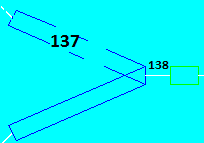
\includegraphics{fig8_ets.PNG}
  \caption{From reverse to forward propagation.}
  \label{fig:min:plus}
\end{marginfigure}
%
%

On \fref{min:plus} is displayed an actual run of \PTC\ using Forest's  Windows$^\text{\textregistered}$ interface. The magnets and drifts in dashed lines have reverse propagators. By looking at \fref{accel.fig8}, where the full Figure-Eight is displayed, the reader can easily spot magnet 137 and drift 138. In this case, the planes are perfectly aligned and, it would appear as in the LHC anecdote, that one does not need a patch. However the $x$-direction of 137 points downwards while on the drift 138 it points upwards. 

\PTC\ puts two patching rotations in this case. The first one is only used when connecting fibres with different directions of propagation; the information is at \lref{bx1:m}. Geometrically it is a rotation of 180 degrees around the $x$-axis. It inverts the $y$ and the $z$ axes. In practice, only $y$ co\"ordonates are inverted since the $z$ direction is not needed for propagation. However this maneuver leaves the $y$ axis pointing in the wrong direction, this is corrected by a \emph{bona fide} phase space rotation around the $z$ axis as shown on \lref{mu:pi}.

It is important to realize that this patch is computed with pure geometrical calculations using the exit frame of 137 and the entrance frame of 138.  The reader may wonder why \PTC 's patching routines did not select a rotation of $\pi $ around the $y$ axis. Rotations around the $x$ and $y$ axis are nonlinear drifts in polar co\"ordinates: they do not make any sense for angles beyond $\pi \over 2$ (See Eq.~\eqref{prot}). Therefore the decomposition of \PTC , while not unique, is necessary.



\endinput


 % modeling accelerators
%!TEX root = ../PTC-LibUG.tex

\chapter{Linking Magnets Together and Moving Them as a Group}
\label{cha:girders}

\fxnote{Review underscore (\_\,) characters in index entries.}
\fxnote{Review percent (\%\,) characters in index entries.}
\fxnote{Review line numbers.}
\fxnote{Say something re misalign v. translate or move. (Or do this in \Cref{geometry}.)}

\index{magnets!linking together}
\index{magnets!moving as group}
\index{Large Hadron Collider!bore magnets}
\index{LHC|see{Large Hadron Collider}}
%
In many accelerator designs, there are groups of elements that move
together as a unit. The Large Hadron Collider, for example, has
dual-bore magnets that carry the two counter-propagating beams through
the cryostats. A more common example is a group of elements assembled
onto a single substrate. When misalignments are applied to
such units, our accelerator modeling code should respect the internal
geometric constraints.

\PTC\ allows us to link elements together to model groups of elements
that move as units. In this chapter, we describe the two tools that
\PTC\ provides---called siamese and girders---and we illustrate their
use by applying them to the collider (layouts \ptc{Col1} and \ptc{Col2})
of the previous chapter.


\section{Siamese and Girders}
\label{sec:siamese.girders}

\index{siamese!defined}
\index{magnet!siamese}
\index{linked list!circular}
\index{siamese!misaligning}
\index{misalignment!siamese}
\index{siamese!frame of reference}
%
A \emph{siamese} consists of elements that are linked together so
that one can move them as a group. Those elements may be in the
same or different layouts. The elements in a siamese are often
parallel, as in a collider; but they may be in different arcs of
a recirculator---arcs, for example, that share common cryogenics.

\begin{marginfigure}[3\baselineskip]\forcerectofloat
  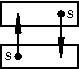
\includegraphics{SiameseGirders/siamgird-01}
  \caption{A pair of elements linked together as a siamese.}
  \label{fig:ll.siamese}
\end{marginfigure}

\begin{marginfigure}
  \includegraphics{SiameseGirders/siamgird-02}\quad
  \includegraphics{SiameseGirders/siamgird-03}
  \caption{Incorrect and correct rotations of a siamese.}
  \label{fig:siamese.rot}
\end{marginfigure}

To create a siamese, we build a circular linked list containing
the several elements we wish to tie together. See \fref{ll.siamese}.
When moving a siamese, \PTC\ traverses the linked list, moving
all the siamese elements in concert. Note that doing this
properly---\ie\ preserving the geometric relations between the
siamese elements---requires the use of a common reference frame.
\fref[c]{siamese.rot}, for example, illustrates incorrect and correct rotations of a pair of elements linked together as a siamese.
In the left-hand graphic of that figure, the same rotation applied
to the \emph{separate} elements breaks the geometry of the siamese.
In the right-hand graphic, the use of a common reference frame when
rotating the elements preserves the geometry. When we link the
elements together as a siamese and then ask \PTC\ to rotate the
siamese---as opposed to the individual elements---\PTC\ takes care
of the details and preserves the internal geometric constraints.
We discuss geometric operations applied to siamese later in this
chapter. See also \TPref*{sec:ops.siamese}.

A siamese does not have an independent reference frame; instead, a
siamese frame is defined in terms of translations and rotations with
respect to the frame of one of its constituent elements. Misalignments
of a siamese are then specified in a similar way with respect to the
siamese frame. If we zero the misalignments, the siamese returns to
its original location.

\index{girder!defined}
\index{magnet!in girder}
\index{girder!misaligning}
\index{misalignment!girder}
\index{girder!frame of reference}
\index{affine\_frame@\ptc{affine\_frame}}
%
A \emph{girder} is a collection of siamese and regular elements
tied to a substrate so that one can move them as a unit. Like a
siamese, we construct a girder as a circular linked list containing
the elements belonging to the common substrate. See \fref{ll.girder}.
Unlike a siamese, a girder typically has its own reference frame,
independent of any element on the girder. This is actually a
\emph{pair} of reference frames---stored in the \PTC\ data type
\ptctyp{affine_frame}. The two frames specify location and
orientation for the original and misaligned girder. This structure
simplifies the process of misaligning a girder: If applying a
\emph{different} misalignment to the girder, \PTC\ starts with
the original frame. If \emph{adding} to an existing misalignment,
\PTC\ uses the misaligned frame as its starting point. If we remove
the misalignment, \PTC\ easily returns the girder to its original
position in the lattice. We discuss geometric operations applied
to girders later in this chapter. See also \TPref*{sec:ops.girders}.

\begin{marginfigure}[-21\baselineskip]\forceversofloat
  \includegraphics{SiameseGirders/siamgird-04}
  \caption{A trio of elements linked together as a girder that
           has its own reference frame.}
  \label{fig:ll.girder}
\end{marginfigure}

Do note that linking together a group of elements on a girder does not mean those elements may no longer move with respect to one another. It is only the geometric operations that apply specifically to girders that will preserve the geometric relations between the girder elements. A similar comment applies for the siamese.

\index{PTC!source file}
\index{source file!geometry tutorial}
\index{geometry!tutorial source file}
\index{z\_ptc\_geometry.f90@\ptc{z\_ptc\_geometry.f90}!geometry tutorial source file}
\index{siamese!creating}
\index{girder!creating}
\index{siamese!misaligning}
\index{misalignment!siamese}
\index{girder!misaligning}
\index{misalignment!girder}
%
In this chapter we show how to create a pair of siamese and a girder
in the collider---trackable layouts \ptc{Col1} and \ptc{Col2} from
\Cref{model.accel}---as well as how to misalign them. The code in
this chapter is from the \PTC\ geometry tutorial source file,
\ptc{ptc_geometry.f90}, which is given in \Aref{geom.tutorial}.
The line numbers of the code shown here refer to the line numbers
of the code in that appendix.


\section{Building Siamese, Girders, and their Reference Frames}

\begin{marginfigure}[2\baselineskip]\forceversofloat
  \includegraphics[]{Layouts/models-08}
  \caption{Collider interaction region. The numbers show the indices
           of a few of the fibres within the corresponding layout.}
  \label{fig:col.intxn}
\end{marginfigure}

\index{move\_to@\ptc{move\_to}!routine}
\index{routine!\ptc{move\_to}}
%
At each end of the straight section shared by layouts \ptc{Col1}
and \ptc{Col2}, see \fref{col.intxn}, is a pair of overlapping bend
magnets. In the first block of code below, we group each pair of bends
as a siamese. For the pair at the left-hand end of the straight,
we set, in the first two lines, pointers \ptc{p1} and \ptc{p2}
respectively to the 67$^\text{th}$ and 7$^\text{th}$ fibres of
layouts \ptc{Col1} and \ptc{Col2}. Those two fibres contain the
pair of elements we wish to group together as a siamese. Each of
those elements---\ptc{p1\%mag} and \ptc{p2\%mag}---contains an
element pointer called \ptc{siamese}. In \lref[s]{siam1.p2} and
\lref*{siam2.p1} we now set each element's \ptc{siamese} pointing
to the other element, thus creating a circular linked list that
ties these two elements together.

In a similar fashion, the next four lines link together as a
siamese the two bends at the right-hand end of the common straight.
Those elements belong to the 4$^\text{th}$ and 70$^\text{th}$
fibres respectively of layouts \ptc{Col1} and \ptc{Col2}.
%
\setptclinenums{386}{5}
\begin{ptccode}
call move_to(Col1, p1, 67)
call move_to(Col2, p2, 7)
p1%mag%siamese => p2%mag    \label{lin:siam1.p2}
p2%mag%siamese => p1%mag    \label{lin:siam2.p1}
call move_to(Col1, p1, 4)
call move_to(Col2, p2, 70)
p1%mag%siamese => p2%mag
p2%mag%siamese => p1%mag
\end{ptccode}

\enlargethispage{\baselineskip}
Our next goal is to group together onto a girder the above two
siamese and all the intervening elements shared by layouts
\ptc{Col1} and \ptc{Col2}. In addition, we will add one more
element to our girder: the bend in the 14$^\text{th}$ fibre of
layout \ptc{Col2} (see upper left of \fref{col.intxn}). We do
this not because this example seems likely from an engineer's
perspective, but because we want to illustrate the flexibility
of \PTC's approach. In particular, we wish to emphasize the
fact that elements tied to a common girder need not be adjacent.
Nevertheless, tied to a common substrate, they will move as a unit.

The next block of code links together the elements we want on our girder. As for the case of siamese, every \PTC\ \ptctyp{element} contains an element pointer called \ptc{girders}, and we use this to construct the linked list that ties our girder elements together. Pointing \ptc{p1} to the short drift at the left-hand end of the common straight section (in fibre~68 of layout \ptc{Col1}), we deal first with the girder elements common to layouts \ptc{Col1} and \ptc{Col2}. In \lref[s]{blp.grdr}--\lref*{elp.grdr}, we march along the straight section, pointing \ptc{p2} to the next fibre, linking the elements in \ptc{p1} and \ptc{p2} (\lref{link.lp}), and then advancing \ptc{p1}. After that loop terminates, both \ptc{p1} and \ptc{p2} point to fibre~4 in layout \ptc{Col1}, and we have linked together the elements of the common straight section plus that last bend.
%
\begin{ptccode}
call move_to(Col1, p1, 68)
pf => p1  ! remember start of girder linked-list
do i = 2, 7                 \label{lin:blp.grdr}
  p2 => p1%next
  p1%mag%girders => p2%mag  \label{lin:link.lp}
  p1 => p1%next
end do                      \label{lin:elp.grdr}
call move_to(Col2, p2,  7)
p1%mag%girders => p1%mag%siamese  \label{lin:grdr.4.70}
p1%mag%siamese%girders => p2%mag  \label{lin:grdr.70.7}
p2%mag%girders => p2%mag%siamese  \label{lin:grdr.7.67}
call move_to(Col1, p1, 67)
call move_to(Col2, p2, 14)
p1%mag%girders => p2%mag          \label{lin:grdr.67.14}
p2%mag%girders => pf%mag           \label{lin:grdr.14.68}
\end{ptccode}
%
In the rest of this block of code, we link in the remaining four
bends we want on our girder: the ones labeled 7, 14, and 70 from
\ptc{Col2}, and 67 from \ptc{Col1}. (Because these four labels are
distinct, we
simplify the following description: instead of saying, for example,
``the bend in fibre~4 of \ptc{Col1}'', we shall say simply ``bend~4''.)
First, we move \ptc{p2} to bend~7. \lref[c]{grdr.4.70} then links
bend~4 to bend~70, because \ptc{p1\%mag\%siamese} already points to
the latter. \lref[c]{grdr.70.7} links bend~70 to bend~7; and
\lref{grdr.7.67} links bend~7 to bend~67, because \ptc{p2\%mag\%siamese}
already points to the latter. It now remains for us to link in
bend~14 and then close our linked list of girder elements. To do
this, we first point \ptc{p1} to bend~67 and \ptc{p2} to bend~14.
Then \lref{grdr.67.14} adds the girder link from one to the other
of those two elements. Finally, \lref{grdr.14.68} closes the linked
list.

We now have a pair of siamese and a girder defined in our collider.
Our next task is to define appropriate siamese and girder frames.
Though we may locate those frames wherever we wish, a sensible choice
for the girder might be to make it coincide with the entrance frame
of the first fibre in layout \ptc{Col1}, at the center of our collider's
common straight section. We accomplish this in the next block of
code.

\index{allocate\_af@\ptc{allocate\_af}!routine}
\index{routine!\ptc{allocate\_af}}
\index{girder\_frame@\ptc{girder\_frame}}
%
\enlargethispage{\baselineskip}
After moving \ptc{p1} to the first fibre in layout \ptc{Col1}, we
then, in \lref{alloc.gf}, allocate memory for the special dual
reference frame needed by our girder, \ptc{p1\%mag\%girder_frame}.%
\sidenote[][-7.5\baselineskip]{Read \ptc{alloc\_af} as ``allocate affine frame''.}
This has four pieces we need to define: \ptc{a} and \ptc{b} for
the origins of the original and current (or misaligned) frames,
and \ptc{ent} and \ptc{exi} for the bases of those two frames.%
\sidenote[][-7.5\baselineskip]{Here the \emph{origin} of a reference
frame refers to a three-dimensional vector that stores the
co\"ordinates of the local frame's origin with respect to the
global frame. The \emph{basis} refers to a $3\times3$ matrix whose
rows contain the orthogonal unit vectors of the local frame, written
with respect to the global frame. See \Cref{geometry} for more details.}
In the remaining four lines of this block of code, we set these
components equal to the corresponding parts (origin or basis) of
the entrance reference frame of the element in fibre \ptc{p1}.
This information is held in \ptc{p1\%mag\%parent_fibre\%chart\%f},
which you might read as ``the magnet frame attached to the chart
associated with this element's parent fibre''.
%
\begin{ptccode}
call move_to(Col1, p1, 1)
call alloc_af(p1%mag%girder_frame, girder = .true.)  \label{lin:alloc.gf}
p1%mag%girder_frame%a   = p1%mag%parent_fibre%chart%f%a
p1%mag%girder_frame%ent = p1%mag%parent_fibre%chart%f%ent
p1%mag%girder_frame%b   = p1%mag%parent_fibre%chart%f%a
p1%mag%girder_frame%exi = p1%mag%parent_fibre%chart%f%ent
\end{ptccode}
%
As set here, the original and current frames are identical,
so this girder is in its design location. Later, if we ask
\PTC\ to misalign this girder, it will modify \ptc{girder_frame\%b}
and \ptc{girder_frame\%exi}, leaving \ptc{girder_frame\%a} and
\ptc{girder_frame\%ent} to record the design location and
orientation of our girder.

\begin{marginfigure}[2\baselineskip]
  \includegraphics{Layouts/models-09}
  \caption{Collider interaction region. The small cross-hairs
           indicate the frame location for each siamese.}
  \label{fig:col.siamfr}
\end{marginfigure}

\index{siamese\_frame@\ptc{siamese\_frame}}
%
In the following block of code, we also define reference frames for
the two siamese. In this case, we choose to locate the siamese frames
along the axis of the common straight section, five meters from the
center of that straight, and oriented parallel to the girder's frame of
reference. (See the cross-hairs in \fref{col.siamfr}.) Consider first
the left-hand siamese: We compute, in \lref[s]{sf.borg}--\lref*{sf.eorg},
the desired origin of our siamese frame. Then, in the following two
lines, we move fibre pointer \ptc{p3} to bend~67 and allocate the
necessary memory.%
\sidenote{This means the siamese frame will be attached to bend~67,
but one could equally well attach it to bend~7, the other magnet in
this siamese.}
Here is where a siamese and girder differ. When \PTC\ allocates a
\emph{girder} frame (by setting \ptc{girder = .true.}, as in
\lref{alloc.gf} above), it allocates memory for the data \ptc{a},
\ptc{ent}, \ptc{b}, and \ptc{exi}. For the siamese frame (the default, as in
\lref{alloc.sf} below,  is \ptc{girder = .false.}) \PTC\ allocates
memory for the data \ptc{d} and \ptc{angle}, which specify not the
frame itself, but rather how to get there (translation and angle)
from the entrance frame of the local element. Our next step is
therefore to compute \ptc{d} and \ptc{angle}. This we do in
\lref{sf.patch} with a call to \ptc{find\_patch}. The first two
arguments are respectively the origin and basis of bend~67's entrance
frame. The second two arguments are the desired origin (\ptc{a}) and
basis (same as for the girder). And the last two arguments are
the computed translation and angle, which we store in our siamese
frame: \ptc{p3\%mag\%siamese_frame\%d} and
\ptc{p3\%mag\%siamese_frame\%angle}.

In a similar fashion, the remaining lines in this block of code
define the reference frame for the other siamese.
%
\begin{ptccode}
a = p1%mag%girder_frame%a                         \label{lin:sf.borg}
a(3) = a(3) - 5.d0                                \label{lin:sf.eorg}
call move_to(Col1, p3, 67)
call alloc_af(p3%mag%siamese_frame)               \label{lin:alloc.sf}
call find_patch(p3%mag%p%f%a, p3%mag%p%f%ent, &   \label{lin:sf.patch}
                a, p1%mag%girder_frame%ent, &
                p3%mag%siamese_frame%d, p3%mag%siamese_frame%angle)
a = p1%mag%girder_frame%a
a(3) = a(3) + 5.d0
call move_to(Col1, p3, 4)
call alloc_af(p3%mag%siamese_frame)
call find_patch(p3%mag%p%f%a, p3%mag%p%f%ent, &
                a, p1%mag%girder_frame%ent, &
                p3%mag%siamese_frame%d, p3%mag%siamese_frame%angle)
\end{ptccode}


\section{Examples of Misalignments}
\label{sec:xmpl.misalign}

The remaining blocks of code in this chapter show some examples of
misalignment operations on the girder and siamese---with variations
in their order and options. In the margin are corresponding figures
that illustrate the effect of the different misalignments. (For
comparison, \fref{col.nomis} shows the same portion of the collider
with no misalignments.) To make the effects clear, we have made very
exaggerated ``misalignments'':
$\SI{\piunit/8}{\radian} = \ang{22.5}$ for rotations, and \SI{2}{m}
for displacements.

The various misalignments are specified by the six-component vector
\ptc{mis}: the first three components describe translation, while
the last three describe rotation in \PTC\ order. This code is
probably only somewhat self-explanatory. Nevertheless, we present
it here for you to look at and mull over, with only a little in the
way of comments. A detailed explanation is given in \CTref*{geometry}.

\begin{marginfigure}[5\baselineskip]\forcerectofloat
  \includegraphics{SiameseGirders/siamgird-mma-0}
  \caption{No misalignment.}
  \label{fig:col.nomis}
\end{marginfigure}

Concerning \lref{moveto.b7}, note that bend~7 (\ie\ the bend contained
in fibre~7 of layout \ptc{Col2}) is present in both the girder and the
left-hand siamese, which are the parts we misalign in the examples
given here. That bend is not \emph{directly} associated with either
the girder frame or the siamese frame. But it is \emph{in}directly
associated: via the linked lists that define the girder and the
siamese, \PTC\ can always find the appropriate girder or siamese frame.
%
\index{misalign\_siamese@\ptc{misalign\_siamese}!routine}
\index{routine!\ptc{misalign\_siamese}}
\index{misalign\_girder@\ptc{misalign\_girder}!routine}
\index{routine!\ptc{misalign\_girder}}
%
\begin{ptccode}
write(6,*) "Example # (from the manual) 1--11 ?"
read(5,*) example
call move_to(Col2, p2, 7) \label{lin:moveto.b7}
if(example == 1) then            \textcolor{DarkRed}{\textsl{! Example 1}}
  mis = 0.d0
  mis(5) = pi / 8.d0
  call misalign_girder(p2, mis)
elseif(example == 2) then        \textcolor{DarkRed}{\textsl{! Example 2}}
  mis = 0.d0
  mis(1) = 2.0d0
  call misalign_girder(p2, mis)
elseif(example == 3) then        \textcolor{DarkRed}{\textsl{! Example 3}}
  mis = 0.d0
  mis(5) = pi / 8.d0
  call misalign_girder(p2, mis)
  mis = 0.d0
  mis(1) = 2.d0
  call misalign_girder(p2, mis, add = .false.)
elseif(example == 4) then        \textcolor{DarkRed}{\textsl{! Example 4}}
  mis = 0.d0
  mis(5) = pi / 8.d0
  call misalign_girder(p2, mis)
  mis = 0.d0
  mis(1) = 2.d0
  call misalign_girder(p2, mis, add = .true.)
elseif(example == 5) then        \textcolor{DarkRed}{\textsl{! Example 5}}
  mis = 0.d0
  mis(1) = 2.d0
  mis(5) = pi / 8.d0
  call misalign_girder(p2, mis)
\end{ptccode}

\begin{marginfigure}[-13.1cm]\forcerectofloat
  \includegraphics{SiameseGirders/siamgird-mma-1}%
  \makebox[0pt]{\textcolor{DarkRed}{1}}\\[14pt]\noindent
  \includegraphics{SiameseGirders/siamgird-mma-2}%
  \makebox[0pt]{\textcolor{DarkRed}{2}}\\[14pt] \noindent
  \includegraphics{SiameseGirders/siamgird-mma-3}%
  \makebox[0pt]{\textcolor{DarkRed}{3}}\\[14pt] \noindent
  \includegraphics{SiameseGirders/siamgird-mma-4}%
  \makebox[0pt]{\textcolor{DarkRed}{4}}\\[14pt] \noindent
  \includegraphics{SiameseGirders/siamgird-mma-5}%
  \makebox[0pt]{\textcolor{DarkRed}{5}}
  \caption{Examples 1 (top) through 5 (bottom).}
\end{marginfigure}

The examples above all misalign only the girder. In the following examples, we apply a misalignment also to one of the siamese. Note that the difference between examples 7 and 8 is solely to the optional argument \ptc{add} in \lref[s]{mis.x7} and \lref*{mis.x8}.
%
\begin{ptccode}
elseif(example == 6) then        \textcolor{DarkRed}{\textsl{! Example 6}}
  mis = 0.d0
  mis(1) = 2.d0
  call misalign_siamese(p2, mis)
elseif(example == 7) then        \textcolor{DarkRed}{\textsl{! Example 7}}
  mis = 0.d0
  mis(1) = 2.d0
  call misalign_siamese(p2, mis)
  mis = 0.d0
  mis(1) = 2.d0
  mis(5) = pi / 8.d0
  call misalign_girder(p2, mis, add = .false.) \label{lin:mis.x7}
elseif(example == 8) then        \textcolor{DarkRed}{\textsl{! Example 8}}
  mis = 0.d0
  mis(1) = 2.d0
  call misalign_siamese(p2, mis)
  mis = 0.d0
  mis(1) = 2.d0
  mis(5) = pi / 8.d0
  call misalign_girder(p2, mis, add = .true.) \label{lin:mis.x8}
elseif(example == 9) then        \textcolor{DarkRed}{\textsl{! Example 9}}
  mis = 0.d0
  mis(1) = 2.d0
  mis(5) = pi / 8.d0
  call misalign_girder(p2, mis)
  mis = 0.d0
  mis(1) = 2.d0
  call misalign_siamese(p2, mis, add = .false.)
elseif(example == 10) then       \textcolor{DarkRed}{\textsl{! Example 10}}
  mis = 0.d0
  mis(1) = 2.d0
  mis(5) = pi / 8.d0
  call misalign_girder(p2, mis)
  mis = 0.d0
  mis(1) = 2.d0
  call misalign_siamese(p2, mis, add = .true.)
elseif(example == 11) then       \textcolor{DarkRed}{\textsl{! Example 11}}
  mis = 0.d0
  mis(1) = 2.d0
  mis(5) = pi / 8.d0
  call misalign_girder(p2, mis)
  mis = 0.d0
  mis(1) = 2.d0
  call misalign_siamese(p2, mis, add = .false., &
                        preserve_girder = .true.)
end if
\end{ptccode}

\begin{marginfigure}[-17.3cm]\forceversofloat
  \makebox[0pt][l]{\textcolor{DarkRed}{6}}%
  \includegraphics{SiameseGirders/siamgird-mma-6}\\[24pt]\noindent
  \makebox[0pt][l]{\textcolor{DarkRed}{7}}%
  \includegraphics{SiameseGirders/siamgird-mma-7}\\[24pt]\noindent
  \makebox[0pt][l]{\textcolor{DarkRed}{8}}%
  \includegraphics{SiameseGirders/siamgird-mma-8}\\[24pt]\noindent
  \makebox[0pt][l]{\textcolor{DarkRed}{9}}%
  \includegraphics{SiameseGirders/siamgird-mma-9}\\[24pt]\noindent
  \makebox[0pt][l]{\textcolor{DarkRed}{10}}%
  \includegraphics{SiameseGirders/siamgird-mma-10}\\[24pt]\noindent
  \makebox[0pt][l]{\textcolor{DarkRed}{11}}%
  \includegraphics{SiameseGirders/siamgird-mma-11}
  \caption{Examples 6 (top) through 11 (bottom).}
\end{marginfigure}


\endinput
 % linking magnets
%!TEX root = ../PTC-LibUG.tex
\linenumberfrequency{5}

\chapter{Taylor Polymorphism and Knobs}
\label{cha:polymorphs.knobs}

\fxnote{Review underscore (\_\,) characters in index entries.}
\fxnote{Review percent (\%\,) characters in index entries.}

\index{Taylor polymorphism!described}
\index{Taylor map!derived from integrator}
\index{integrator!Taylor map}
\index{FPP!defined}
\index{FPP!documentation}
%
\PTC\ supports the full usage of Taylor maps derived from the integrator for the computation of lattice functions. \PTC\ uses \FPP, a package of polymorphic types and tools to extract and analyze the Taylor maps.
Information explaining \FPP%
\footnote{The CERN folder is called \ptc{PTC_proper} to distinguish it from the information on \MadX. Most of the information in the \ptc{PTC_proper} folder is about \FPP.}
is at \url{http://mad.web.cern.ch/mad/PTC\_proper/}


\section{Polymorphs}

\index{polymorph!defined}
%
A \emph{polymorph} is the \Fninety\ type \ptctyp{real_8}:

\linenumberfrequency{0}
\begin{ptccode}
type real_8
  type (taylor) :: T   ! active if Taylor
  real(dp) :: r        ! active if real or knob
  integer :: kind      ! 1=real,2=Taylor,3=Taylor knob,0=special
  integer :: i         ! used for knobs
  real(dp) :: s        ! scaling for knobs
  logical(lp) :: alloc ! is Taylor is allocated in DA-package?
end type real_8
\end{ptccode}

Polymorphs allow the computation of parameter-dependent maps.


\subsection{States of a Polymorph}

\index{polymorph!states}
%
A polymorph \ptc{Y} can be
real (\ptc{Y\%kind = 1}),
Taylor (\ptc{Y\%kind = 2}),
or a special Taylor called a \emph{knob} (\ptc{Y\%kind = 3}).


\subsection{Computing a Taylor Map}

\index{Taylor map!computing}
%
Suppose we have a closed orbit at position 1 given by six real numbers \ptc{fix(1:6)}. We can construct the following array of six polymorphs:

\begin{ptccode}
type(real_8) :: Y(6)
type(damap) :: id

call init(state, NO, 0)
call alloc(Y)
call alloc(id)

id = 1
Y = fix + id
\end{ptccode}

The variable \ptc{state} describes internal states of \PTC.

The variable \ptc{id} is a differential algebra map (\ptc{damap}), and \ptc{id = 1} constructs the identity map.

Then \ptc{Y = fix + id} creates the polymorphic component \ptc{Y(i)} given by \ptc{Y(i) = fix(i) + $x_i$}, where $x_i$ denotes the $i$-th component of the identity map \ptc{id}.

\index{one-turn map!computing}
\index{TRACK@\ptc{TRACK}!routine}
\index{routine!\ptc{TRACK}}
%
To compute a one-turn map, for example, we track \ptc{Y} around the
machine (here \ptc{R}) as if it were six real numbers:

\begin{ptccode}
call track(R, Y, 1, state)
\end{ptccode}

\index{internal states!setting}
\index{state!internal}
%
At the end, \ptc{Y} contains the Taylor map, to order \ptc{NO}, about the closed orbit \ptc{fix}. The internal state variable \ptc{state} determines the exact nature of the map:
\begin{enumerate}
  \item \ptc{state = default0} specifies a 6-D map with cavities;
  \item \ptc{state = default0 + nocavity0} specifies a 6-D map with cavities skipped;
  \item \ptc{state = default0 + only\_4d0} specifies a 4-D phase space $(X, P_X, Y, P_Y)$;
  \item \ptc{state = default0 + delta0} specifies a 4-D phase
space $(X, P_X, Y, P_Y)$, plus energy as the fifth variable; cavities are skipped.
\end{enumerate}

For more information about states, see \Aref{states}.


\section{Knobs}

\index{knob!defined}
\index{polymorph!knob}
%
A \emph{knob} is a polymorph that turns itself into a simple Taylor
series when used. A knob cannot be on the left side of an equal sign.

Knobs let users set up parameters that can be changed without having to recompile.


\subsection{Using Knobs}

\index{knob!using}
%
Example: The \ptc{bn(2)} (quadrupole component) of a magnet is
made into the first knob:

\begin{ptccode}
bn(2)%kind = 3
bn(2)%i = 1
bn(2)%s = 1
\end{ptccode}

At execution time, during an operation involving \ptc{bn(2)}, the
knob becomes the following Taylor map:

\begin{ptccode}
bn(2)= bn(2)%r + bn(2)%s * X_j
\end{ptccode}

In the map above, \ptc{j= npara_fpp + bn(2)\%i}.

The integer \ptc{npara_fpp} depends on the state: It equals
the minimal number of variables compatible with the state selected.
In the four \ptc{state} examples above:
\begin{enumerate}
  \item \ptc{npara_fpp = 6} $\Rightarrow$ \ptc{j = 7}
  \item \ptc{npara_fpp = 6} $\Rightarrow$ \ptc{j = 7}
  \item \ptc{npara_fpp = 4} $\Rightarrow$ \ptc{j = 5}
  \item \ptc{npara_fpp = 5} $\Rightarrow$ \ptc{j = 6}
\end{enumerate}


\subsection{Creating Knobs}

\index{knob!creating}
%
While \FPP\ has a routine to help users make a knob, \PTC\ has tailored
routines to put knobs into a layout and remove knobs from a layout.
%
\index{scan\_for\_polymorphs@\ptc{scan\_for\_polymorphs}!routine}
\index{routine!\ptc{scan\_for\_polymorphs}}
%
The types, subroutines, and routines are
\begin{itemize}
  \item \ptc{type pol_block};
  \item subroutine \ptc{scan_for_polymorphs(R,B)} or \ptc{R = B};
  \item unary \ptc{+}, as in \ptc{+state}, to activate knobs in a \ptc{track} routine;
  \item \ptc{TPSAfit(1:lnv)} array;
  \item \ptc{set_TPSAfit} and \ptc{set_element} logicals;
  \item subroutine \ptc{kill_para_L(R)}.
\end{itemize}
For more information about the unary \ptc{+} used to activate knobs in
a \ptc{track} routine, see \TAref*{states}.


\subsection{Polymorphic Blocks}

\index{polymorphic block!described}
\index{block|see{LEGO block \emph{or} polymorphic block}}
%
This section discusses type \ptc{pol\_block}, setting values for
polymorphic blocks, and removing polymorphic blocks from layouts.


\subsubsection{Type \ptc{pol_block}}

\index{pol\_block@\ptc{pol\_block}!data type}
\index{data type!\ptc{pol\_block}}
%
This data type creates an object to be compared with an actual layout. It identities families or single elements using the name, part of the name, or the \ptc{vorname} (first name) of an element to make certain variables knobs. (The last name is the family, for example: \ptc{QF}.)

\begin{ptccode}
type pol_block
  character(nlp) name
  integer :: n_name
  character(vp) vorname

  ! types for setting magnet using global array TPSAfit
  real(dp), dimension(:), pointer :: TPSAfit
  logical(lp), pointer :: set_TPSAfit
  logical(lp), pointer :: set_element

  ! types for parameter dependence
  integer :: npara ! should not be used anymore

  ! knob index
  integer ::  ian(nmax), ibn(nmax)
  real(dp) :: san(nmax), sbn(nmax)
  integer :: ivolt, ifreq, iphas
  integer :: ib_sol

  ! scales for knobs
  real(dp) :: svolt, sfreq, sphas
  real(dp) :: sb_sol

  ! user defined functions
  type(pol_block_sagan) :: SAGAN
end type pol_block
\end{ptccode}

Consider the following \ptc{pol\_block qf}:
\begin{ptccode}
qf = 0         ! initialize the pol_block qf
qf%name = 'QF' ! specify a family name
qf%ibn(2) = 1  ! set normal quad strength as first parameter
\end{ptccode}
%
\index{scan\_for\_polymorphs@\ptc{scan\_for\_polymorphs}!routine}
\index{routine!\ptc{scan\_for\_polymorphs}}
%
If we call the routine \ptc{scan_for_polymorphs(R, qf)} or \ptc{R = qf}, then the \DNA\ layout \ptc{R} is scanned. If a polymorphic magnet on any fibre of the layout \ptc{R} is named \ptc{'QF'}, then \ptc{bn(2)} becomes a knob. In our example:
\begin{verbatim}
  bn(2) = bn(2%r + qf%sbn(2) * X(fpp_npara) + qf%ibn(2)
  bn(2) = bn(2)%r + X(fpp_npara) + 1
\end{verbatim}
The index \ptc{fpp_npara} depends on the state as explained above.

One may also specify an integer \ptc{qf\%n_name}. If, for example, \ptc{qf\%n_name = 2}, then a polymorph is set if the magnet name matches \ptc{'QFxxxxxxxxxxxxxxx'}, where \ptc{x} denotes any character.

Once the knobs are set on the lattice using the routine \ptc{scan\_for\_polymorphs}, tracking routines can be invoked after the DA-package has been initialized.


\subsubsection{Setting Values using Polymorphic Blocks}

\index{polymorphic block!setting values}
%
Polymorphs allow for the computation of parameter-dependent maps. These maps can be analyzed by various methods including normal forms. From these maps one may attempt to fit certain computed quantities by modifying the parameters of the polymorphs on the ring.

\index{scan\_for\_polymorphs@\ptc{scan\_for\_polymorphs}!routine}
\index{routine!\ptc{scan\_for\_polymorphs}}
\index{SET\_TPSAFIT@\ptc{SET\_TPSAFIT}!routine}
\index{routine!\ptc{SET\_TPSAFIT}}
\index{SET\_ELEMENT@\ptc{SET\_ELEMENT}!routine}
\index{routine!\ptc{SET\_ELEMENT}}
%
This is done as follows with \ptc{scan_for_polymorphs} or the
= sign assignment. The global parameter \ptc{set_TPSAfit} turns
the \ptc{scan_for_polymorphs} routine into a routine that inputs
the array \ptc{TPSAfit(1:C_\%np_pol)} into variables that the
\ptc{pol_block}s make into knobs. Note that the knobs exist only
in the polymorphic version of the magnet located at \ptc{fibre\%magp}.
The polymorphic version is copied into the real magnet \ptc{fibre\%mag} if \ptc{set_element} is true.

\begin{ptccode}
set_TPSAfit = .true.
set_element = .true.
Col1%DNA(1)%L = qf(1)
Col1%DNA(1)%L = qd(1)
Col1%DNA(2)%L = qf(2)
Col1%DNA(2)%L = qd(2)
set_element = .false.
set_TPSAfit = .false.
\end{ptccode}


\subsubsection{Removing Polymorphic Blocks from Layouts}

\index{polymorphic block!removing from layout}
\index{KILL\_PARA@\ptc{KILL\_PARA}!routine}
\index{routine!\ptc{KILL\_PARA}}
%
To remove a polymorphic block from a layout use the subroutines
\begin{ptccode}
call kill_para(Col1%DNA(1)%L)
call kill_para(Col1%DNA(2)%L)
\end{ptccode}


\section{Tutorial Example}
\linenumberfrequency{5}

\index{PTC!source file}
\index{source file!polymorphs and knobs tutorial}
\index{polymorph!tutorial source file}
\index{knob!tutorial source file}
\index{z\_ptc\_geometry.f90@\ptc{z\_ptc\_geometry.f90}!geometry tutorial source file}
%
The example code in this chapter is from the \PTC\ geometry tutorial source file, \ptc{ptc_geometry.f90}, which is given in \Aref{geom.tutorial}. The line numbers of the code in the examples refer to the line numbers of the code in the appendix.

This tutorial example shows how to create a map for the collider with polymorphs and knobs.

The first six lines of code initialize the polymorphic block for the
focusing quadrupoles (\ptc{qf}) in \ptc{Col1} and \ptc{Col2},
give the quadrupoles the family name \ptc{'QF'}, and set
their normal strength as the first parameter in the Taylor series. The following six lines do the same for the defocusing quadrupoles (\ptc{'QD'}).

\setptclinenums{313}{5}
\begin{ptccode}
qf(1) = 0
qf(1)%name = 'qf'
qf(1)%ibn(2) = 1
qf(2) = 0
qf(2)%name = 'qf'
qf(2)%ibn(2) = 3
qd(1) = 0
qd(1)%name = 'qd'
qd(1)%ibn(2) = 2
qd(2) = 0
qd(2)%name = 'qd'
qd(2)%ibn(2) = 4
\end{ptccode}

\index{scan\_for\_polymorphs@\ptc{scan\_for\_polymorphs}!routine}
\index{routine!\ptc{scan\_for\_polymorphs}}
%
The next four lines of code declare \ptc{qf} and \ptc{qd} as independent in \DNA\ layouts \ptc{L5} and \ptc{L6}. They perform the same function as calls to the subroutine \ptc{scan_for_polymorphs}. If a polymorphic magnet on any fibre of the DNA layouts \ptc{L5} and \ptc{L6} is named \ptc{'QF'} or \ptc{'QD'}, then \ptc{ibn(2)} becomes a knob.

\begin{ptccode}
Col1%dna(1)%L = qf(1)
Col1%dna(1)%L = qd(1)
CoL1%dna(2)%L = qf(2)
CoL1%dna(2)%L = qd(2)
\end{ptccode}

Once the knobs are set on the lattice using the \ptc{scan\_for\_polymorphs} routine (or equivalent), we can invoke tracking routines after the
DA-package has been initialized.

The following lines of code define the closed orbit if not 0.

\setptclinenums{330}{5}
\begin{ptccode}
101 continue
state = default0 + only_4d0

fix1 = 0.d0
fix2 = 0.d0;
call init(state, 2, c_%np_pol) ! c_%np_pol is automatically computed
\end{ptccode}

The \ptc{2} is automatically computed above---counting the number of
\DNA\ variables (1-4). This means the Taylor series now has eight variables.

\index{FIND\_ORBIT@\ptc{FIND\_ORBIT}!routine}
\index{routine!\ptc{FIND\_ORBIT}}
%
\begin{ptccode}
call find_orbit(CoL1, fix1, 1, state, 1.d-6)
call find_orbit(Col2, fix2, 1, state, 1.d-6)
call alloc(y1)
call alloc(y2)
call alloc(id)
call alloc(n1)
call alloc(n2)
call alloc(eq);
id=1 ! identity damap
y1 = id + fix1 ! this is permitted in ptc only (not fpp)
y2 = id + fix2 ! closed orbit added to map
\end{ptccode}

The plus sign in the next two lines of code activates the knobs.
If we remove the plus sign, \PTC\ will ignore the knobs.

\index{TRACK@\ptc{TRACK}!routine}
\index{routine!\ptc{TRACK}}
%
\begin{ptccode}
call track(Col1, y1, 1, +state) ! unary + activates knobs
call track(Col2, y2, 1, +state)
\end{ptccode}

\index{normal form!computing}
\index{tune!computing}
%
After accounting for knobs, the code computes the tunes (with and
without knobs). Equations 1 and 2 compute the tunes for \ptc{col1};
equations 3 and 4 compute the tunes for \ptc{col2}.

The first number is the difference between the goal and what we have
obtained, which should be as close to 0 as possible.

\begin{ptccode}
n1 = y1 ! normal forms: abused of language permitted by ptc
n2 = y2 ! normally one should do => damap=y; normalform=damap
write(6,*) " tunes 1 "
write(6,*) n1%tune(1:2)
write(6,*) " tunes 2 "
write(6,*) n2%tune(1:2)
eq(1) = n1%dhdj%v(1) - 0.254d0
eq(2) = n1%dhdj%v(2) - 0.255d0
eq(3) = n2%dhdj%v(1) - 0.130d0
eq(4) = n2%dhdj%v(2) - 0.360d0
do i = 1, 4
  eq(i) = eq(i) <= c_%npara
end do

call kanalnummer(mf,"eq.txt")
do i=1,4
  call daprint(eq(i), mf)
end do
close(mf)

call kill(y1)
call kill(y2)
call kill(id)
call kill(n1)
call kill(n2)
call kill(eq)
call init(1,4)
call alloc(g,4)
call kanalnummer(mf,"eq.txt")
do i = 1, 4
  call read(g%v(i), mf)
end do
close(mf)

g = g.oo.(-1)
tpsafit(1:4) = g
set_tpsafit = .true.
set_element = .true.
Col1%dna(1)%L = qf(1)
Col1%dna(1)%L = qd(1)
Col1%dna(2)%L = qf(2)
Col1%dna(2)%L = qd(2)
set_tpsafit = .false.
set_element = .false.
call kill(g)
\end{ptccode}

We need to kill the knobs after we compute them: the two calls to
\ptc{kill_para} kill the knobs in \DNA\ layouts \ptc{L5} and
\ptc{L6}.

\begin{ptccode}
write(6,*) " more "
read(5,*) i
if(i == 1) goto 101
call kill_para(Col1%dna(1)%l)
call kill_para(Col1%dna(2)%l)
\end{ptccode}

\endinput
 % polymorphism and knobs
%!TEX root = ../PTC-LibUG.tex
\linenumberfrequency{0}

\chapter{Computing Accelerator Properties}
\label{cha:accel.properties}

\index{accelerator!properties}
\index{property!accelerator}
This chapter explains how to compute global and local accelerator
properties and provides examples of the code required for the computations.


\section{Global Scalars}

\index{global property!described}
\index{property!global}
\index{global property|see{\emph{also} global information}}
\index{closed orbit!global properties}
%
Global scalars apply to the accelerator as a whole. They can be
derived only after the complete accelerator has been modeled, and
they are the same at any point on the closed orbit.


\subsection{Tunes}

\begin{ptccode}
x = zero
x(5) = delta
call find_orbit(lattice, x, 1, istate, 1.d-7)
call init(istate, 1, 0)
call alloc(y)
call alloc(normal)
call alloc(id)
id = 1
y = x + id
call track(lattice, y, 1, istate)
normal = y
write(6,'(a,3(2x,f9.6))') 'tunes:', normal%tune
\end{ptccode}


\subsection{Chromaticity}

%\begin{ptccode}
%\end{ptccode}


\subsection{Anharmonicity}

%\begin{ptccode}
%\end{ptccode}


\section{s-Dependent Global Quantities}

\subsection{Betatron Amplitude}

\begin{ptccode}
x = zero
x(5) = delta
call find_orbit(lattice, x, 1, istate, 1.d-7)
call init(istate, 1, 0)
call alloc(y)
call alloc(normal)
call alloc(id)
id = 1
y = x + id
call track(lattice, y, 1, istate)
normal = y
y = x + normal%a_t  ! track this---normalizing transformation
p => lattice%start
beta_x = (y(1).sub.'10') ** 2   + (y(1).sub.'01') ** 2
beta_y = (y(3).sub.'0010') ** 2 + (y(3).sub.'0001') ** 2
write(6,'(a,2(2x,f9.6))') 'beta_x, beta_y: ', beta_x, beta_y
do j = 1, lattice%n
  call track(lattice, y ,j, j+1, istate)
  beta_x = (y(1).sub.'10') ** 2   + (y(1).sub.'01') ** 2
  beta_y = (y(3).sub.'0010') ** 2 + (y(3).sub.'0001') ** 2
  write(6,'(a,2(2x,f9.6))') 'beta_x, beta_y: ', beta_x, beta_y
  p => p%next
end do
\end{ptccode}


%\subsection{Twiss Parameter}

%\begin{ptccode}
%\end{ptccode}


\subsection{Dispersion}

\begin{ptccode}
x = zero
x(5) = delta
call find_orbit(lattice, x, 1, istate, 1.d-7)
call alloc(id)      ! type(damap)
call alloc(disp)    ! type(damap)
call alloc(xt)      ! type(damap)
call alloc(eta)     ! type(real_8), dimension(6)
call alloc(y)       ! type(real_8), dimension(6)
call alloc(normal)  ! type(normalform)
id = 1
y = x + id
call track(lattice, y, 1, default)
normal = y
y = x + normal%A_t
p => lattice%start
do j = 1, lattice%n
  call track(lattice, y ,j, j+1, default)
  id = 0
  xt = y
  disp = xt * id
  x = xt
  id = 1
  disp = id - disp
  xt = disp * xt
  eta = x + xt
  dispx = (eta(1).sub.'00001')
  dispy = (eta(3).sub.'00001')
  write(6,'(a,2(2x,f9.6))') 'disp_x, disp_y: ', dispx, dispy
end do
\end{ptccode}


\subsection{Phase Advance}

\begin{marginfigure}
  \centering
  \includegraphics{MetaPost/PhaseAdvance/phaseadv-01}
  \caption{One-turn and partial-turn transfer maps.}
  \label{fig:maps-ring}
\end{marginfigure}

\begin{figure}[htbp]
  \centering
  \includegraphics{MetaPost/PhaseAdvance/phaseadv-02}
  \caption{This graphic illustrates the essential relationships between the one-turn map and the normal form at two different locations in a ring lattice.}
  \label{fig:geom-phsadv}
\end{figure}

See caveat at end of \Sref{analyze.accel.prop}!

\begin{ptccode}
x = zero
x(5) = delta
call find_orbit(lattice, x, 1, istate, 1.d-7)
call init(istate, 1, 0)
call alloc(y)
call alloc(normal)
call alloc(id)
id = 1
y = x + id
call track(lattice, y, 1, istate)
normal = y
y = x + normal%a_t
theta_prev = zero
phi = zero
write(6,'(a,2(2x,f9.6))') ' CS phase adv:', phi(1:2)
p => lattice%start
do j = 1, lattice%n
  call track(lattice, y ,j, j+1, istate)
  theta(1) = atan2((y(1).sub.'01'), (y(1).sub.'10')) / twopi
  theta(2) = atan2((y(3).sub.'0001'), (y(3).sub.'0010')) / twopi
  do k = 1, 2
    if(theta(k) < zero .and. abs(theta(k)) > tiny) then
      theta(k) = theta(k) + one
    end if
    dphi(k) = theta(k) - theta_prev(k)
    if(dphi(k) < zero .and. abs(dphi(k)) > tiny) then
      dphi(k) = dphi(k) + one
    end if
    phi(k) = phi(k) + dphi(k)
  end do
  theta_prev = theta
  write(6,'(a,2(2x,f9.6))') ' CS phase adv:', phi(1:2)
  p => p%next
end do
\end{ptccode}


\subsection{Beam Envelope}

Text and example code here.
%\begin{ptccode}
%\end{ptccode}


\section{Local Quantities}

\index{local property!described}
\index{property!local}
\index{local property|see{\emph{also} local information}}
\index{closed orbit!local properties}
%
Local properties do not apply to the accelerator as a whole. They
are derived from individual magnets, and they differ at different
points on the closed orbit. The trajectory of a particle through a
magnet is local; it is derivable from the individual magnet irrespective
of the magnet's position in the accelerator.

\endinput
 % computing accelerator properties
%!TEX root = ../PTC-LibUG.tex

\chapter{Tracking Routines}
\label{cha:tracking}

\index{routines!tracking}
\index{tracking routines!list of}
%
\PTC's tracking routines are divided into four categories:

\begin{itemize}
  \item standard tracking routines on fibres,
  \item tracking routines on integration nodes,
  \item tracking routines on 3-D information through an integration node,
  \item time-based tracking routines.
\end{itemize}

A fifth section documents the closed-orbit routine.

Mandatory arguments for the tracking routines are in
\ptc{regular black} type. Optional arguments are in \ptc{\textit{\textcolor{red}{red italic}}} type.

\index{one-turn map!creating}
%
Positions are normally specified by \ptc{I1}, \ptc{I2}, \ptc{fibre1},
\ptc{fibre2}, \ptc{node1}, or \ptc{node2}. Generally, if only
\ptc{x1} is present (\ptc{x=I}, \ptc{fibre}, or \ptc{node}), this produces a
one-turn map from position \ptc{x1} back to position \ptc{x1} if the layout
is closed. If the layout is opened, then it goes to the end of the line.

If \ptc{x1} and \ptc{x2} are present, the routine tracks through \ptc{x1} all
the way to the front of \ptc{x2} (\ptc{x2} not included).

The only exception to all of this is the time-based tracking routine.

\fxnote{Al: \'Etienne mentioned that we should discuss spinors in relation to tracking routines.}


\section{Standard Tracking Routines on Fibres}

\index{routines!standard tracking}
\index{tracking routines!standard}
\index{routines!tracking fibres}
\index{tracking routines!fibres}
\index{spin!tracking routines on fibres}
\index{radiation!tracking routines on fibres}
\index{tracking routines!spin}
\index{tracking routines!radiation}
\index{fibre!tracking routines}
%
These routines do not support spin and radiation.


\subsection{Track}

\index{track@\ptc{track}!routine}
\index{routine!\ptc{track}}
%
\begin{ptccode}
track (R, X\textit{\textcolor{red}{, I1, I2}}, K)
\end{ptccode}

\ptc{X} is an array of six \ptc{real(dp)} or \ptc{REAL\_8}.

\ptc{I1} and \ptc{I2} are the position of the fibres.

\ptc{Result=TRACK\_FLAG (R,X,I1,I2,k)}

\ptc{Result=logical}; true indicates stable; false indicates unstable.

\begin{ptccode}
track (C, X, K\textit{\textcolor{red}{, CHARGE}})
\end{ptccode}

This routine tracks through the fibre \ptc{C}.


\subsection{Find\_orbit}

\index{find\_orbit@\ptc{find\_orbit}!routine}
\index{routine!\ptc{find\_orbit}}
%
\begin{ptccode}
find_orbit(R, FIX, LOC, STATE, eps\textit{\textcolor{red}{, TURNS}})
\end{ptccode}

The \ptc{find\_orbit} routine works in the same way as the
subroutine \ptc{find\_orbit\_x} but on the fibre structure
without radiation. For more information about the subroutine
\ptc{find\_orbit\_x}, see \Tref{sub:Find-Orbit-X}.

\ptc{LOC} is the integer location in the layout \ptc{R}.


\section{Tracking Routines on Integration Nodes}

\index{routines!tracking integration nodes}
\index{tracking routines!integration nodes}
\index{spin!tracking routines on integration nodes}
\index{radiation!tracking routines on integration nodes}
\index{tracking routines!spin}
\index{tracking routines!radiation}
\index{integration node!tracking routines}
%
These routines support spin and radiation.


\subsection{Routines for Tracking either Probe or Probe\_8}

\index{probe!tracking routines}
%
For the type definitions of \ptc{probe} and \ptc{probe\_8}, see
\Tref{sub:Probe-B}.


\subsubsection{TRACK\_PROBE2}

\index{TRACK\_PROBE2@\ptc{TRACK\_PROBE2}!routine}
\index{routine!\ptc{TRACK\_PROBE2}}
%
\begin{ptccode}
TRACK_PROBE2(R,XS,K\textit{\textcolor{red}{,I1,I2}})
\end{ptccode}

\ptc{I1,I2 = NODE POSITION}

\ptc{I1} only implies a one-turn map.

\ptc{K=INTERNAL STATE}


\subsubsection{TRACK\_PROBE}

\index{TRACK\_PROBE@\ptc{TRACK\_PROBE}!routine}
\index{routine!\ptc{TRACK\_PROBE}}
%
\begin{ptccode}
TRACK_PROBE (R,XS,K\textit{\textcolor{red}{,FIBRE1,FIBRE2,NODE1,NODE2}})
\end{ptccode}

\ptc{FIBRE1,FIBRE2,NODE1,NODE2} are all integer positions of either the
fibre or the integration node.


\subsubsection{TRACK\_NODE\_PROBE}

\index{TRACK\_NODE\_PROBE@\ptc{TRACK\_NODE\_PROBE}!routine}
\index{routine!\ptc{TRACK\_NODE\_PROBE}}
%
\begin{ptccode}
TRACK_NODE_PROBE(T,XS,K)
\end{ptccode}

\ptc{T} is an integration node.


\subsubsection{Object-Oriented Routines}

\index{routines!object-oriented}
\index{tracking routines!object-oriented}
\index{TRACK\_PROBE2@\ptc{TRACK\_PROBE2}!routine}
\index{routine!\ptc{TRACK\_PROBE2}}
\index{TRACK\_PROBE@\ptc{TRACK\_PROBE}!routine}
\index{routine!\ptc{TRACK\_PROBE}}
\index{TRACK\_NODE\_PROBE@\ptc{TRACK\_NODE\_PROBE}!routine}
\index{routine!\ptc{TRACK\_NODE\_PROBE}}
%
\begin{ptccode}
TRACK_PROBE2 (XS,K\textit{\textcolor{red}{,FIBRE1,FIBRE2,NODE1,NODE2}})
TRACK_PROBE (XS,K\textit{\textcolor{red}{,FIBRE1,FIBRE2,NODE1,NODE2}})
TRACK_NODE_PROBE (XS,K\textit{\textcolor{red}{,FIBRE1,FIBRE2,NODE1,NODE2}})
\end{ptccode}

These are all calls to the same routine. The fibres and the nodes
are actual pointers to the objects.

\index{one-turn map!tracking}
%
One turn can be done as follows:

\begin{ptccode}
TRACK_PROBE (XS,K\textit{\textcolor{red}{,NODE1=T,NODE2=T%PREVIOUS}})
\end{ptccode}

\index{routine!\ptc{TRACK\_PROBE\_X}}
\index{TRACK\_PROBE\_X@\ptc{TRACK\_PROBE\_X}!routine}
%
In the \ptc{TRACK\_PROBE\_X} routine, the fibres and the nodes are pointers to the objects.
The routine wraps the \ptc{TRACK\_PROBE} routine shown above.

\begin{ptccode}
TRACK_PROBE_X (R,X,K,U,T\textit{\textcolor{red}{,FIBRE1,FIBRE2,NODE1,NODE2}})
\end{ptccode}

\fxnote{Al: Is my rewording above correct? What does ``wrap'' mean? Will the meaning be clear to our audience?}


\subsection{Routines for Tracking either Real or Real\_8}

All these routines wrap the above routines and therefore support radiation,
beam-beam and $s$-dependent apertures.


\subsubsection{TRACK\_NODE\_X}

\index{routine!\ptc{TRACK\_NODE\_X}}
\index{TRACK\_NODE\_X@\ptc{TRACK\_NODE\_X}!routine}
%
\begin{ptccode}
TRACK_NODE_X(T,X,K)
\end{ptccode}

\subsubsection{TRACK\_PROBE\_X}

\index{routine!\ptc{TRACK\_PROBE\_X}}
\index{TRACK\_PROBE\_X@\ptc{TRACK\_PROBE\_X}!routine}
%
\begin{ptccode}
TRACK_PROBE_X(R,X,K\textit{\textcolor{red}{,U,T,FIBRE1,FIBRE2,NODE1,NODE2}})
\end{ptccode}

\ptc{U=LOGICAL} where \ptc{TRUE} indicates \ptc{UNSTABLE} (optional).

\ptc{T} is a pointer to the fibre where the particle is lost (optional).


\subsubsection{TRACK\_BEAM}

\index{routine!\ptc{TRACK\_BEAM}}
\index{TRACK\_BEAM@\ptc{TRACK\_BEAM}!routine}
\index{tracking routines!beam of particles}
%
This routine tracks a beam of particles.

\begin{ptccode}
TRACK_BEAM(R,B,K\textit{\textcolor{red}{,T,FIBRE1,FIBRE2,NODE1,NODE2}})
\end{ptccode}

For the type definition of \ptc{BEAM}, see Section~\ref{sub:Beam-B}.


\section{Tracking Routines on 3-D Information through an Integration Node}

\index{routines!tracking integration nodes}
\index{tracking routines!integration nodes}
\index{tracking routines!3-D information through integration node}
\index{integration node!tracking routines}
%
These routines track three-dimensional information through an integration node.


\subsection{Track\_node\_v}

\index{routine!\ptc{TRACK\_NODE\_V}}
\index{TRACK\_NODE\_V@\ptc{TRACK\_NODE\_V}!routine}
%
The \ptc{TRACK\_NODE\_V} routine tracks a trajectory and records its
three-dimensional position for plotting at the beginning and the end of a node.

\begin{ptccode}
TRACK_NODE_V (T,V,K,REF)
\end{ptccode}

\ptc{T} is an integration node.

\ptc{V} is of type \ptc{THREE\_D\_INFO}. The type definition is given below.

\index{routine!\ptc{TRACK\_FILL\_REF}}
\index{TRACK\_FILL\_REF@\ptc{TRACK\_FILL\_REF}!routine}
%
\ptc{REF=TRUE} or \ptc{FALSE}. If \ptc{REF=TRUE}, then the results of the
\ptc{TRACK\_FILL\_REF} routine are used. The ray is magnified by 
\ptc{V\%SCALE} (see type \ptc{THREE\_D\_INFO} below) with respect to a
trajectory computed and stored by the \ptc{TRACK\_FILL\_REF} routine,
which tracks the ray \ptc{FIX} from fibre \ptc{I1} back to fibre \ptc{I1}.

\begin{ptccode}
TRACK_FILL_REF(R,FIX,I1,K))
\end{ptccode}

\index{data type!\ptc{THREE\_D\_INFO}}
\index{THREE\_D\_INFO@\ptc{THREE\_D\_INFO}!data type}
\index{three-dimensional information!data type}
\index{3-D information|see{three-dimensional information}}
%
Here is the data type definition for three-dimensional information.

\begin{ptccode}
TYPE THREE_D_INFO
  REAL(DP) A(3),B(3)         ! CENTRE OF ENTRANCE AND EXIT FACES
  REAL(DP) ENT(3,3),EXI(3,3) ! ENTRANCE AND EXIT FRAMES FOR DRAWING MAGNET FACES
  REAL(DP) WX,WY             ! WIDTH OF BOX FOR PLOTTING PURPOSES
  REAL(DP) O(3),MID(3,3)     ! FRAMES AT THE POINT OF TRACKING
  REAL(DP) REFERENCE_RAY(6)  !
  REAL(DP) X(6)              ! RAY TRACKED WITH REFERENCE_RAY USING A TYPE(BEAM)
  REAL(DP) R0(3),R(3)        ! RAY POSITION GLOBAL RETURNED
  REAL(DP) SCALE             ! MAGNIFICATION USING REFERENCE_RAY
  LOGICAL(LP) U(2)           ! UNSTABLE FLAG FOR BOTH RAY AND REFERENCE_RAY
END TYPE THREE_D_INFO
\end{ptccode}


\section{Time-based Tracking Routines}

\index{routines!time-based tracking}
\index{tracking routines!time-based}
%
These routines provide time-based tracking of temporal probes and temporal beams.


\subsection{Track\_time}

\index{routine!\ptc{TRACK\_TIME}}
\index{TRACK\_TIME@\ptc{TRACK\_TIME}!routine}
%
\begin{ptccode}
TRACK_TIME(XT,DT,K)
\end{ptccode}

\ptc{XT} is a temporal probe. For the type definition of \ptc{TEMPORAL\_PROBE},
see Section~\ref{sub:Temporal-Probe-B}.


\subsection{Track\_temporal\_beam}

\index{routine!\ptc{TRACK\_TEMPORAL\_BEAM}}
\index{TRACK\_TEMPORAL\_BEAM@\ptc{TRACK\_TEMPORAL\_BEAM}!routine}
%
\begin{ptccode}
TRACK_TEMPORAL_BEAM(B,DT,STATE)
\end{ptccode}

\ptc{B} is a temporal beam. For the type definition of \ptc{TEMPORAL\_BEAM},
see Section~\ref{sub:Temporal-Beam-B}.


\section{Closed-Orbit Routine}

\index{closed orbit!finding}
%
This routine finds the closed orbit.


\subsection{Find\_orbit\_x}
\label{sub:Find-Orbit-X}

\index{routine!\ptc{FIND\_ORBIT\_X}}
\index{FIND\_ORBIT\_X@\ptc{FIND\_ORBIT\_X}!routine}
%
\begin{ptccode}
FIND_ORBIT_X(R,FIX,STATE,eps\textcolor{red}{,TURNS,fibre1,node1})
\end{ptccode}

Here \ptc{fibre1} and \ptc{node1} are integer positions. The routine finds the
fixed point for \ptc{TURNS} turns; one turn if not specified.

The argument \ptc{eps= real(dp)} number is used to do numerical
differentiation---typically \ptc{1.d-6} works.

For a no-cavity fixed point, \ptc{fix(5)} must contain the energy variable.

\endinput
 % tracking routines
%!TEX root = ../PTC-LibUG.tex

\chapter{Geometric Routines}
\label{cha:geometry}

\fxnote{Need to proof-read geometric formulas.}
\fxnote{Could we make the red italic type less glaring?}

\index{routines!geometric}
\index{geometric routines!described}
%
\PTC's geometric routines are divided into three categories:
\begin{itemize}
  \item affine routines on pure geometry,
  \item affine routines on computer objects,
  \item dynamical routines.
\end{itemize}

Mandatory arguments for the geometric routines are in \ptc{regular
black} type.  Optional arguments are in \ptc{\textit{\textcolor{red}{red
italic}}} type.


\section{Affine Routines on Pure Geometry}

\index{affine routines!on pure geometry}
\index{routines!affine}
\index{affine basis!geometric routines}
\index{global frame!geometric routines}
%
Affine routines on pure geometry act on a pure geometrical affine basis:
\ptc{A(3)} and \ptc{V(3,3)} where \ptc{A} represents the coordinates of a
point in the global frame, and \ptc{V(3,3)} the coordinates of a triad of vectors.


\subsection{Theory}
\label{sub:Theory-Affine-Routines}

\index{affine routines!theory}
%
Consider a point $a$ and vector basis $(v_1,v_2,v_3)$ attached
to a solid (a magnet, for example). See \fref{Rotating-point-a}.

\begin{figure}[ht]
  \centering
  \includegraphics{illustrations/geo-routines-1}
  \caption{Rotating point $a$ and vector basis $(v_1,v_2,v_3)$ by $R$.}
  \label{fig:Rotating-point-a}
\end{figure}

The vector $a$ can be expressed as follows:
\begin{equation*}
  a = \sum_i  a_i v_i.
\end{equation*}

The basis vectors $v_i$ can be expressed in terms of a global basis, that is, \PTC's global frame:
\begin{equation*}
  v_i = \sum_j V_{ij} e_j.
\end{equation*}
 
Suppose we rotate the solid by a rotation $R$ defined by its action on the basis
$(v_1,v_2,v_3)$:
\begin{equation*}
  w_i = R v_i = \sum_j R_{ij} v_j.
\end{equation*}

Then we ask the following question: what are the components of $w_i$ in the global basis $(e_1,e_2,e_3)$ in terms of the component array $V_{ij}$?

Note: The components of $b$ in the frame $(w_1,w_2,w_3)$,
which is the image of $a$ upon rotation of the magnet, are
also given $a_i$ because this point is fixed in the magnet.

Solution:
\begin{equation*}
 w_i = R v_i = \sum_j R_{ij} v_j = \sum_{jk} R_{ij} V_{jk} e_k = \sum_k W_{ik} e_k.
\end{equation*}

Thus we have
\begin{equation*}
  W = RV.
\end{equation*}

The components of the vector $b$ in the global frame are then
\begin{equation*}
  b_k = \sum_{ij} a_i R_{ij} V_{jk} e_k
  \rightarrow b = (RV)^t a.
\end{equation*}

We now address a slightly harder problem, which is essential in \PTC.
The rotation $R$, instead of being defined in the frame $(v_1,v_2,v_3)$,
might be defined on a totally different frame $(u_1,u_2,u_3)$:
\begin{equation*}
  u_i = \sum_k U_{ik} e_k.
\end{equation*}
Therefore, prior to rotating the basis $(v_1,v_2,v_3)$, we must
express it in the frame $(u_1,u_2,u_3)$:
\begin{equation*}
  a = \sum_{ik} a_i V_{ik} e_k
    = \sum_{ikn} a_i V_{ik} U^{-1}_{kn} u_n
    = \sum_{ikn} a_i V_{ik} U_{nk} u_n.
\end{equation*}

We can now apply the rotation $R$ defined on the basis $(u_1,u_2,u_3)$:
\begin{equation*}
  b = \sum_{iknm} a_i V_{ik} U_{nk} R_{nm} u_m
    = \sum_{iknm} a_i V_{ik} U_{nk} R_{nm} U_{mk} e_k.
\end{equation*}

Thus the final result of $W$ is:
\begin{equation*}
  W = VU^t RU
\end{equation*}

The point $b$ in global coordinates is:
\begin{equation*}
  b_i = \sum_k a_i W_{ik}
  \rightarrow b = (VU^t RU)^t a.
\end{equation*}

Notice that if $V=U$, we regain the previous result.

\PTC\ factors the rotation $R$ in the form
\begin{equation*}
  R = R_z R_y R_x
\end{equation*}

Using local variables results in the need to go back and forth between frames.
The magnets must be placed within the global frame. However, the tracking is
in local variables. We need routines that are able to connect geometrically
both points of view.


\subsection{Descriptions of the Routines}

This section describes the affine routines on pure geometry.


\subsubsection{GEO\_ROT}

\begin{ptccode}
GEO_ROT(V(3, 3),W(3, 3),A(3),B(3),ANG(3)\textit{\textcolor{red}{,BASIS(3,3)}})
\end{ptccode}

\index{routine!\ptc{GEO\_ROT}}
\index{GEO\_ROT@\ptc{GEO\_ROT}!routine}
%
This routine exactly reproduces the theory in the previous section.

\ptc{BASIS} is an optional variable, which is set equal to the $U$ described
in Section~\ref{sub:Theory-Affine-Routines}.

The real array \ptc{ANG(3)} is used to define $R$:
\begin{equation*}
R = R_z (ang(3)) R_y (ang(2)) R_x (ang(1))
\end{equation*}

\begin{ptccode}
GEO_ROT(V(3, 3),W(3, 3),ANG(3)\textit{\textcolor{red}{,BASIS(3,3)}})
\end{ptccode}

This routine is the same as the previous routine except that
\ptc{A} and \ptc{B} are not needed.

\begin{ptccode}
GEO_ROT(V(3, 3),A(3),ANG(3),I\textit{\textcolor{red}{,BASIS(3,3)}})
\end{ptccode}

Here the final $W$ and $B$ are copied back into $V$ and $A$. The
integer \ptc{I} can be $\pm1$ to produce the inverse rotation: $R^{\pm1}$.

\begin{ptccode}
GEO_ROT(V(3, 3),ANG(3),I\textit{\textcolor{red}{,BASIS(3,3)}})
\end{ptccode}

This routine is the same as the previous routine without the \ptc{A} vector.


\subsubsection{GEO\_TRA}

\begin{ptccode}
GEO_TRA(A(3),V(3, 3) (3),D,I)
\end{ptccode}

\index{routine!\ptc{GEO\_TRA}}
\index{GEO\_TRA@\ptc{GEO\_TRA}!routine}
%
\ptc{A} is translated by $\pm$ \ptc{D} expressed in the basis \ptc{V}; \ptc{I} = $\pm1$.
\begin{equation*}
  \text{result} = \sum_{ij} (a_j e_j \pm d_i V_{ij} e_j)
\end{equation*}

The result is put back in \ptc{A}, that is:
\begin{equation*}
  A \leftarrow A \pm V^t D
\end{equation*}


\subsubsection{Rotating and Translating the Frames of a Magnet}

\begin{ptccode}
ROTATE_FRAME(F,OMEGA,ANG,ORDER\textit{\textcolor{red}{,BASIS(3,3)}})
\end{ptccode}

\index{translation routines!described}
\index{rotation routines!described}
\index{routine!\ptc{ROTATE\_FRAME}}
\index{ROTATE\_FRAME@\ptc{ROTATE\_FRAME}!routine}
%
\ptc{F} is of type \ptc{magnet\_frame} and contains three affine frames tied
to the magnet.
\begin{equation*}
F = \lbrace ( F \% A(3), F \% ENT(3) ), ( F \% O(3), F \% MID(3) ), ( F \% B(3), F \% EXI(3) ) \rbrace
\end{equation*}

The entire content of \ptc{F} is rotated as shown in \fref{Rotating-and-translating}.

\begin{figure}[ht]\forceversofloat
  \centering
  \includegraphics{illustrations/geo-routines-2}
  \caption{Rotating and translating the frames of a magnet.}
  \label{fig:Rotating-and-translating}
\end{figure}

\index{routine!\ptc{TRANSLATE\_FRAME}}
\index{TRANSLATE\_FRAME@\ptc{TRANSLATE\_FRAME}!routine}
%
\begin{ptccode}
TRANSLATE_FRAME(F,D,ORDER\textit{\textcolor{red}{,BASIS(3,3)}})

CALL CHANGE_BASIS(D,BASIS,DD,GLOBAL_FRAME)

P%A = P%A + ORDER * DD
P%B = P%B + ORDER * DD
P%O = P%O + ORDER * DD
\end{ptccode}

The frame is simply translated by \ptc{D}. The translation \ptc{D} is expressed
in \ptc{BASIS} if present.


\subsubsection{CHANGE\_BASIS}

\index{routine!\ptc{CHANGE\_BASIS}}
\index{CHANGE\_BASIS@\ptc{CHANGE\_BASIS}!routine}
%
\begin{ptccode}
CHANGE_BASIS(A(3),V(3,3),B(3),W(3,3))
\end{ptccode}

The component vector \ptc{A}, expressed in the basis \ptc{V}, is re-expressed
as \ptc{B} using basis \ptc{W}. \ptc{B} is the output of this subroutine.
\begin{equation*}
  \sum_{ik} a_i V_{ik} e_k = \sum_{ik} b_i W_{ik} e_k
  \rightarrow b = WV^t a.
\end{equation*}


\subsubsection{COMPUTE\_ENTRANCE\_ANGLE}

\index{routine!\ptc{COMPUTE\_ENTRANCE\_ANGLE}}
\index{COMPUTE\_ENTRANCE\_ANGLE@\ptc{COMPUTE\_ENTRANCE\_ANGLE}!routine}
%
\begin{ptccode}
COMPUTE_ENTRANCE_ANGLE(V(3,3),W(3,3),ANG(3))
\end{ptccode}

\index{rotation!order of}
%
This is a crucial routine. Given two frames \ptc{V} and \ptc {W}, which most likely
represent a magnet or a beam line, the routine computes a rotation
$R$ in the standard \PTC\ order, that is,
\begin{equation*}
  R = R_z (\ptc{ang(3)}) R_y (\ptc{ang(2)}) R_x (\ptc{ang(1)})
\end{equation*}
such that \ptc{V} is transformed into \ptc{W}. It is the reverse routine from \ptc{GEO\_ROT}.


\subsubsection{FIND\_PATCH\_B}

\index{routine!FIND\_PATCH\_B@\ptc{FIND\_PATCH\_B}}
\index{FIND\_PATCH\_B@\ptc{FIND\_PATCH\_B}!routine}
\index{patching!FIND\_PATCH\_B@\ptc{FIND\_PATCH\_B} routine}
\index{patch!inserting}
%
This routine connects the affine frame \ptc{A,V} to the affine frame \ptc{B,W}.

\begin{ptccode}
FIND_PATCH_B(A(3),V(3,3),B(3),W(3,3),D(3),ANG(3))
\end{ptccode}

\begin{ptccode}
SUBROUTINE FIND_PATCH_B(A,V,B,W,D,ANG)
  !\ FINDS PATCH BETWEEN V AND W : INTERFACED LATER FOR FIBRES
  IMPLICIT NONE
  REAL(DP), INTENT(INOUT) ::\ V(3,3),W(3,3)
  REAL(DP), INTENT(INOUT) ::\ A(3),B(3),D(3),ANG(3)
  CALL COMPUTE_ENTRANCE_ANGLE(V,W,ANG)
  D=B-A; CALL CHANGE_BASIS(D,GLOBAL_FRAME,D,W);
END SUBROUTINE FIND_PATCH_B
\end{ptccode}

The above code is a simple example of the usage of the geometric routines.
This geometric routine is very close to the dynamical set up of \PTC. Patches
are written as an ``x'' rotation, a ``y'' rotation, a ``z'' rotation, followed by a
translation (transverse + drift). Note that the translation $D = B - A$ between
is expressed in the final frame $W$. This is normal if dynamical rotations
precede the translations.


\subsubsection{FIND\_INVERSE\_PATCH}

\index{routine!\ptc{INVERSE\_FIND\_PATCH}}
\index{INVERSE\_FIND\_PATCH@\ptc{INVERSE\_FIND\_PATCH}!routine}
\index{patching!\ptc{INVERSE\_FIND\_PATCH} routine}
\index{patch!inserting}
%
This routine is the precise inverse of the \ptc{FIND\_PATCH\_B} routine.
The affine frame \ptc{B,W} is the output.

\begin{ptccode}
INVERSE_FIND_PATCH(A(3),V(3,3),D(3),ANG(3),B(3),W(3,3))
\end{ptccode}

\begin{ptccode}
SUBROUTINE INVERSE_FIND_PATCH(A,V,D,ANG,B,W)
  !\ USED IN MISALIGNMENTS OF SIAMESE
  IMPLICIT NONE
  REAL(DP), INTENT(INOUT)::\ V(3,3),W(3,3)
  REAL(DP), INTENT(INOUT)::\ A(3),B(3),D(3),ANG(3)
  REAL(DP) ::\  DD(3)
  W=V
  CALL GEO_ROT(W,ANG,1,BASIS=V)
  CALL CHANGE_BASIS(D,W,DD,GLOBAL_FRAME)
  B=A+DD
END SUBROUTINE INVERSE_FIND_PATCH
\end{ptccode}


\section{Affine Routines on Computer Objects}

\index{affine routines!on computer objects}
\index{routines!affine}
\index{affine basis!geometric routines}
%
Affine routines on \PTC's computer objects act on the affine bases of magnets,
siamese, girders, integration nodes, and fibres. These objects contain
a myriad of affine bases to help us locate the trajectories in 3-D.

Within this category are two subcategories:
\begin{itemize}
  \item \emph{Affine Routines on Fibrous Structures:} Displacements
that correspond to the design positioning and thus requiring patching.
  \item \emph{Misalignment Routines:} Misalignments representing errors
that do not require patching. The misalignments displace the magnet away
from a fibre that contains it. The misalignments also displace girders
away from their original position.
\end{itemize}


\subsection{Affine Routines on Fibrous Structures}

\index{affine routines!on fibrous structures}
\index{routines!affine}
%
We discussed in the previous section \PTC's geometric tools on the
affine frame. This is useful in giving a pictorial representation of a ring
in 3-D. One can imagine linking \PTC\ with a CAD program equipped
with a magnet widget containing at least one affine frame, say the
cord frame \ptc{O(3), MID(3,3)} of a \PTC\ magnet.

Of course, \PTC\ is dynamically a more complex structure than just
magnets: fibres, integration nodes, layouts, etc. All these objects
have affine frames attached to them, and we must be able to move them.

\index{MAD8!discussed}
%
We describe first the routines that displace \PTC\ structures away from
a standard ``MAD8'' configuration.%
\footnote{The quotation marks indicate that there is really nothing standard
about the so-called standard implicit geometry of MAD8. It is worth
pointing out that the code MAD of CERN and the code SAD of KEK have
different implicit geometry once vertical magnets are invoked: nothing
is standard.%
} These are used in the generation of ``non-standard'' systems.


\subsubsection{Patching Routines}

\index{patching!routines}
\index{patching routines!described}
%
The central power of \PTC\ is its ability to place magnets in arbitrary
positions. To do so, the concept of a fibre with a patch is necessary.


\subsubsection*{FIND\_PATCH}

\index{routine!\ptc{FIND\_PATCH}}
\index{FIND\_PATCH@\ptc{FIND\_PATCH}!routine}
\index{patching!\ptc{FIND\_PATCH} routine}
\index{patch!inserting}
%
\begin{ptccode}
FIND_PATCH(EL1\textit{\textcolor{red}{,EL2_NEXT,NEXT,ENERGY_PATCH,PRECi}})
\end{ptccode}

\ptc{EL1} and \ptc{EL2\_NEXT}

\index{patching!energy}
\index{energy!patch}
%
\ptc{PREC} is a small \ptc{real(dp)} number.  If the norm of the geometric patch is
smaller than \ptc{PREC}, then the patch is ignored. If \ptc{energy\_patch} is true,
then it compares the design momenta of the magnets in both fibres. If the magnitude
of difference is greater than \ptc{PREC}, then an energy patch is put on.


\subsubsection*{CHECK\_NEED\_PATCH}

\index{routine!\ptc{CHECK\_NEED\_PATCH}}
\index{CHECK\_NEED\_PATCH@\ptc{CHECK\_NEED\_PATCH}!routine}
\index{patching!\ptc{CHECK\_NEED\_PATCH} routine}
\index{patch!checking whether needed}
%
This routine checks whether a patch is needed without actually applying
it to the layout. The routine returns the integer \ptc{PATCH\_NEEDED}.
If zero, it is not needed.

\begin{ptccode}
CHECK_NEED_PATCH(EL1,\textit{\textcolor{red}{EL2_NEXT,}}PREC,PATCH_NEEDED)
\end{ptccode}


\subsubsection{Fibre Content}

Before going any further, we remind the reader of the frames contained
within a fibre:
\begin{itemize}
  \item the frames of the fibre itself located in type \ptc{chart}, that is, \ptc{fibre\%chart\%f},
  \item the frames of the magnet \ptc{fibre\%mag\%p\%f} and its polymorphic twin,
  \item the frames of the integration nodes associated with this fibre/magnet,
if they are present,
  \item the frame of a girder that might be tagged on this magnet.
\end{itemize}


\subsubsection{Subroutines Invoking the Magnet and Relying on the DNA}

\index{data type!\ptc{MAD\_UNIVERSE}}
\index{MAD\_UNIVERSE@\ptc{MAD\_UNIVERSE}!data type}
%
When complex structures are constructed in \PTC, it is preferable to follow
a strict discipline. First various layouts with no ``cloning'' of magnets are created
in a ``mad universe'' of data type \ptc{MAD\_UNIVERSE}. The code MAD-X calls this
universe \ptc{M\_U}.

\index{DNA sequence!populating DNA database}
\index{DNA database!populating}
%
These no-clone layouts contain the actual magnet database of the accelerator
complex. Therefore we refer to these layouts as the DNA of the complex.

\index{routine!\ptc{APPEND\_POINT}}
\index{APPEND\_POINT@\ptc{APPEND\_POINT}!routine}
\index{routine!\ptc{APPEND\_EMPTY}}
\index{APPEND\_EMPTY@\ptc{APPEND\_EMPTY}!routine}
\index{routine!\ptc{APPEND\_FIBRE}}
\index{APPEND\_FIBRE@\ptc{APPEND\_FIBRE}!routine}
%
Then trackable structures are appended after the DNA. Since the magnets
of these structures must be in the DNA, they are created with the
\ptc{APPEND\_POINT} routine rather than the standard \ptc{APPEND\_EMPTY}
or \ptc{APPEND\_FIBRE} used for the DNA production.

\index{data type!\ptc{FIBRE\_APPEARANCE}}
\index{FIBRE\_APPEARANCE@\ptc{FIBRE\_APPEARANCE}!data type}
%
When the \ptc{APPEND\_POINT} routine is used, a magnet will automatically
retain memory of its various fibre appearances though a data type called
\ptc{FIBRE\_APPEARANCE}.

\begin{ptccode}
TYPE FIBRE_APPEARANCE
  TYPE(FIBRE), POINTER :: PARENT_FIBRE
  TYPE(FIBRE_APPEARANCE), POINTER :: NEXT
END TYPE FIBRE_APPEARANCE
\end{ptccode}

\index{pointer!\ptc{DOKO}}
\index{DOKO@\ptc{DOKO}!pointer}
\index{doko!described}
\index{linked list!appearances of magnet}
%
Each magnet of the DNA contains a pointer called:

\begin{ptccode}
TYPE(FIBRE_APPEARANCE), POINTER :: DOKO
\end{ptccode}

which constitutes a linked list storing all the appearances of this
magnet in the pointer \ptc{parent\_fibre}. The linked list is terminated,
or grounded, at the last fibre appearance. If more trackable structures
are created, this linked list is extended for each magnet.

There are all sorts of reasons why we may have multiple appearances
of a DNA magnet: recirculation, common section of colliders or even
multiple trackable structures of the same physical object.

It is through the \ptc{DOKO} construct that the following routines know
where all the magnets are located.


\subsubsection{Translation Routines with No Automatic Patching}

\index{translation routines!described}
%
This section describes translation routines that do not automatically patch 
fibres together.


\subsubsection*{TRANSLATE\_FIBRE}

\index{routine!\ptc{TRANSLATE\_FIBRE}}
\index{TRANSLATE\_FIBRE@\ptc{TRANSLATE\_FIBRE}!routine}
%
This routine uses the \ptc{DOKO} construct, if associated, to locate
all the appearances of a magnet and rotate the frames on all integration
nodes if present.

\begin{ptccode}
TRANSLATE_FIBRE(R,D(3)\textit{\textcolor{red}{,ORDER,BASIS(3,3),DOGIRDER}})
\end{ptccode}

Here \ptc{R} is a fibre to be translated by \ptc{D}. \ptc{Dogirder=true} forces the
translation of the girder frame if present.


\subsubsection*{TRANSLATE\_LAYOUT}

\index{routine!\ptc{TRANSLATE\_LAYOUT}}
\index{TRANSLATE\_LAYOUT@\ptc{TRANSLATE\_LAYOUT}!routine}
%
This routine
\begin{itemize}
  \item scans the layout \ptc{R} from position \ptc{I1} to \ptc{I2} inclusive if
present. \ptc{I1} and \ptc{I2} are defaulted to $1$ and $R \% N$ respectively.
  \item calls \ptc{TRANSLATE\_FIBRE} with \ptc{dogirder=true}
on each fibre.
  \item uses the \ptc{DOKO} construct, if associated, to locate all the appearances
of a magnet and rotate the frames on all integration nodes if present.
\end{itemize}

\begin{ptccode}
TRANSLATE_LAYOUT(R,D\textit{\textcolor{red}{,I1,I2,ORDER,BASIS}})
\end{ptccode}


\subsubsection{Rotation Routines with No Automatic Patching}

\index{rotation routines!described}
%
This section describes rotation routines that do not automatically patch 
fibres together.


\subsubsection*{ROTATE\_FIBRE}

\index{routine!\ptc{ROTATE\_FIBRE}}
\index{ROTATE\_FIBRE@\ptc{ROTATE\_FIBRE}!routine}
%
The comments that apply to \ptc{TRANSLATE\_FIBRE} also apply to
\ptc{ROTATE\_FIBRE}.

\begin{ptccode}
ROTATE_FIBRE(R,OMEGA,ANG\textit{\textcolor{red}{,ORDER,BASIS,DOGIRDER}})
\end{ptccode}


\subsubsection*{ROTATE\_LAYOUT}

\index{routine!\ptc{ROTATE\_LAYOUT}}
\index{ROTATE\_LAYOUT@\ptc{ROTATE\_LAYOUT}!routine}
%
The comments that apply to \ptc{TRANSLATE\_LAYOUT} also apply to
\ptc{ROTATE\_LAYOUT}.

\begin{ptccode}
ROTATE_LAYOUT(R,OMEGA,ANG\textit{\textcolor{red}{,I1,I2,ORDER,BASIS}})
\end{ptccode}


\subsubsection{DNA-Designed Rotation Routines with Automatic Patching}

\index{rotation routines!described}
%
This section describes rotation routines that automatically patch fibres together.
The routines have been designed to rotate magnets stored in the DNA database.


\subsubsection*{ROTATE\_MAGNET}

\index{routine!\ptc{ROTATE\_MAGNET}}
\index{ROTATE\_MAGNET@\ptc{ROTATE\_MAGNET}!routine}
%
\begin{ptccode}
ROTATE_MAGNET(R,ANG,OMEGA\textit{\textcolor{red}{,ORDER,BASIS,PATCH,PREC}})
\end{ptccode}

\ptc{R} is a magnet. The routine rotates \ptc{parent\_fibre}, which rotates
all the frames of the magnet.

If \ptc{patch=true}, then all the appearances of this magnet stored in
\ptc{DOKO} are patched---provided the norm of the patches is greater than
\ptc{PREC}. It is advisable to set \ptc{PREC} to a not too small number
(for example, 10$^{-10}$) to avoid useless patches.

If there is no DNA, that is, if \PTC\ runs in pure compatibility mode
with standard codes, then patches are on the parent fibre of the magnet.


\subsubsection*{TRANSLATE\_MAGNET}

\index{routine!\ptc{TRANSLATE\_MAGNET}}
\index{TRANSLATE\_MAGNET@\ptc{TRANSLATE\_MAGNET}!routine}
%
This routine operates like \ptc{ROTATE\_MAGNET} described above.

\begin{ptccode}
TRANSLATE_MAGNET(R,D\textit{\textcolor{red}{,ORDER,BASIS,PATCH,PREC}})
\end{ptccode}


\subsubsection{Operations on Siamese}
\label{sec:ops.siamese}

For a discussion of siamese, see \Sref{siamese.girders}.

\index{pointer!\ptc{SIAMESE}}
\index{SIAMESE@\ptc{SIAMESE}!pointer}
%
Siamese are tied together by the pointer \ptc{SIAMESE}, which
sits on \ptc{fibre\%mag\%siamese}.

\index{siamese!creating}
%
To create a siamese structure, we make a circular linked list of magnets.
For example, suppose three DNA fibres \ptc{f1}, \ptc{f2}, and \ptc{f3} must
be tied together. This can be done as follows:

\begin{ptccode}
f1%mag%siamese=>f2%mag
f2%mag%siamese=>f3%mag
f3%mag%siamese=>f1%mag
\end{ptccode}


\subsubsection*{Siamese Frame of Reference}

\index{siamese!frame of reference}
\index{frame of reference!siamese}
\index{siamese!affine frame}
\index{affine frame!siamese}
\index{routine!\ptc{ALLOC\_AF}}
\index{ALLOC\_AF@\ptc{ALLOC\_AF}!routine}
\index{routine!\ptc{FIND\_PATCH}}
\index{FIND\_PATCH@\ptc{FIND\_PATCH}!routine}
%
Because a siamese does not have its own frame of reference, it is 
advisable to set up a so-called \ptc{affine\_frame} on the siamese.
In the above example, one picks up any magnet of the siamese,
for example \ptc{f1\%mag}, and calls the routine:

\begin{ptccode}
CALL ALLOC_AF(F1%MAG%SIAMESE_FRAME)
CALL FIND_PATCH(\textcolor{green}{F1%CHART%F%A,F1%CHART%F%ENT}\textcolor{red}{,A,ENT},\&
                \textcolor{blue}{F1%MAG%SIAMESE_FRAME%D,F1%MAG%SIAMESE_FRAME%ANGLE})
\end{ptccode}

The siamese frame is located in relative coordinates from the entrance
of the fibre that contains the magnet on which \ptc{siamese\_frame} is
attached (green objects above). Generally we may know the desired
frame of reference in absolute coordinates given by the red \ptc{A(3)}
and \ptc{ENT(3,3)} above. The relative translation and rotation can be
computed, and the result is stored in the blue variables.


\subsubsection*{ROTATE\_SIAMESE}

\index{siamese!rotating}
\index{routine!\ptc{ROTATE\_SIAMESE}}
\index{ROTATE\_SIAMESE@\ptc{ROTATE\_SIAMESE}!routine}
%
This routine rotates the siamese by a set of angles \ptc{ang(1:3)} in the
usual \PTC\ order.

\begin{ptccode}
ROTATE_SIAMESE(S2,ANG\textit{\textcolor{red}{,OMEGA,ORDER,BASIS,PATCH,PREC}})
\end{ptccode}

\ptc{S2} is any fibre that contains an element of the siamese string. The
intricate usage of the optional variables \ptc{OMEGA,ORDER,BASIS} is
best explained by displaying the actual code:

\begin{ptccode}
CALL FIND_AFFINE_SIAMESE(S2,CN,FOUND)
IF(FOUND) CALL FIND_FRAME_SIAMESE(CN,B,EXI,ADD=MY_FALSE)

IF(PRESENT(BASIS)) THEN
  BASIST=BASIS
ELSE
  IF(FOUND) THEN
    BASIST=EXI
  ELSE
    BASIST=GLOBAL_FRAME
  ENDIF
ENDIF
IF(PRESENT(OMEGA)) THEN
  OMEGAT=OMEGA
ELSE
  IF(FOUND) THEN
    OMEGAT=B
  ELSE
    OMEGAT=GLOBAL_ORIGIN
  ENDIF
ENDIF
\end{ptccode}

If \ptc{OMEGA} is present, then it is used. If \ptc{BASIS} is present, it is also
used. Normally one would expect both to be present or both to be absent.
\PTC\ does not check for this.

If they are not present, \PTC\ looks for a siamese frame which is then
used if it exists. Otherwise the global frame is used.

This routine calls the equivalent ``magnet'' routines over the entire string
of siamese, and this permits automatic patching.


\subsubsection*{TRANSLATE\_SIAMESE}

\index{siamese!translating}
\index{routine!\ptc{TRANSLATE\_SIAMESE}}
\index{TRANSLATE\_SIAMESE@\ptc{TRANSLATE\_SIAMESE}!routine}
%
This routine functions like the above \ptc{rotate\_siamese} with the same
priorities concerning the optional variable \ptc{BASIS}.

\begin{ptccode}
TRANSLATE_SIAMESE(S2,D\textit{\textcolor{red}{,ORDER,BASIS,PATCH,PREC}})
\end{ptccode}


\subsubsection{Operations on Girders}
\label{sec:ops.girders}

For a discussion of girders, see \Sref{siamese.girders}.

\index{girder!creating}
%
To create a girder structure, we make a circular linked list of magnets.
Let us create a girder structure with the three siamese \ptc{f1}, \ptc{f2},
and \ptc{f3} above. In addition, let us put a single magnet \ptc{f0} on the girder.

\begin{ptccode}
f0%mag%girder => f1%mag
f1%mag%girder => f2%mag
f2%mag%girder => f3%mag
f3%mag%girder => f0%mag
\end{ptccode}

Four magnets are on the girder; three are in a siamese as well as on the girder.


\subsubsection*{Girder Frame of Reference}

\index{girder!frame of reference}
\index{frame of reference!girder}
\index{girder!affine frame}
\index{affine frame!girder}
\index{routine!\ptc{ALLOC\_AF}}
\index{ALLOC\_AF@\ptc{ALLOC\_AF}!routine}
%
Unlike a siamese, a girder has a frame of reference. For example, we
may elect to put the frame of reference on \ptc{f0}:

\begin{ptccode}
CALL ALLOC_AF(F0%MAG%GIRDER_FRAME,GIRDER=.TRUE.)
\end{ptccode}

Then we set the following two affine frames of the girder to the same
value:

\begin{ptccode}
F0%MAG%GIRDER_FRAME%\textcolor{red}{ENT} = ENT
F0%MAG%GIRDER_FRAME%\textcolor{red}{A} = A
F0%MAG%GIRDER_FRAME%\textcolor{red}{EXI} = ENT
F0%MAG%GIRDER_FRAME%\textcolor{red}{B} = A
\end{ptccode}

The affine frame \ptc{A,ENT} can be any convenient frame chosen by the
people who align the girder on the floor of the machine.

If a girder is misaligned, the affine frame \ptc{B,EXI} contains
the new position of the girder. If the misalignments are removed,
then \ptc{B,EXI} coincides with \ptc{A,ENT}. This allows the girder to have
an existence independent of the fibres themselves. One can move fibres
within a girder during its creation while keeping this frame fixed.


\subsubsection*{ROTATE\_GIRDER and TRANSLATE\_GIRDER}

\index{girder!rotating}
\index{routine!\ptc{ROTATE\_GIRDER}}
\index{ROTATE\_GIRDER@\ptc{ROTATE\_GIRDER}!routine}
\index{girder!translating}
\index{routine!\ptc{TRANSLATE\_GIRDER}}
\index{TRANSLATE\_GIRDER@\ptc{TRANSLATE\_GIRDER}!routine}
%
The routines operate exactly as the siamese routines do and therefore
do not require any special description. The routines describe ``design''
displacements of the girder and therefore the affine frames \ptc{A,ENT}
and \ptc{B,EXI} are moved together.

\begin{ptccode}
ROTATE_GIRDER(S2,ANG\textit{\textcolor{red}{,OMEGA,ORDER,BASIS,PATCH,PREC}})
TRANSLATE_GIRDER(S2,D\textit{\textcolor{red}{,ORDER,BASIS,PATCH,PREC}})
\end{ptccode}


\subsection{Misalignment Routines}

\index{misalignment!routines}
\index{misalignment routines!described}
\index{misalignment!element}
\index{misalignment!siamese}
\index{misalignment!girder}
\index{element!misaligning}
\index{siamese!misaligning}
\index{girder!misaligning}
%
\PTC\ has three fundamental misalignment routines related to a single
magnet, a siamese, and a girder.

The single magnet and the siamese are defined with respect to their
fibre position and are thus inherently similar. The girder has a special
frame of reference independent of the fibre.

If one is not careful, a single magnet or a siamese misalignment may
break the girder. To avoid this problem, we start with the girder misalignment.


\subsubsection{MISALIGN\_GIRDER}

\index{routine!\ptc{MISALIGN\_GIRDER}}
\index{MISALIGN\_GIRDER@\ptc{MISALIGN\_GIRDER}!routine}
%
\begin{ptccode}
MISALIGN_GIRDER(S2,S1\textit{\textcolor{red}{,OMEGA,BASIS,ADD}})
\end{ptccode}

To understand how the misalignments affect single magnets, siamese, 
and girders, we examine the following:
\begin{itemize}
  \item example 0---girder,
  \item example 1---girder after rotation and additive misalignment,
  \item example 2---misalign siamese followed by misalign girder,
  \item example 3---misalign girder followed by misalign siamese,
  \item example 4---misalign siamese with \ptc{PRESERVE\_GIRDER=.true.}.
\end{itemize}

In these examples, we assume that a girder frame of reference has been defined;
otherwise the girder becomes simply a giant siamese.


\subsubsection*{Example 0}

\begin{figure}[ht]
  \centering
  \includegraphics[width=.9\textwidth]{illustrations/misalign-fig1}
  \caption{Example 0: girder.}
  \label{fig:Example-0}
\end{figure}

On the image in \fref{Example-0}, the red and the cyan magnets
are part of a single girder. The origin of the girder frame of reference is
located in the middle of the red drift and displayed with an orange cross.

\index{rotation!order of}
%
The cyan magnets form two siamese: one on the left and one on the
right. The array \ptc{MIS(1:6)} contains the actual misalignments: the translations
in \ptc{MIS(1:3)} and the rotations in \ptc{MIS(4:6)}. They are applied in the
standard \PTC\ order: rotation around the $x$, then the $y$, and finally
the $z$-axis, followed by the translation.


\subsubsection*{Example 1}

Now we rotate the girder by 22.5 degrees, as shown in \fref{Example-1-1}.

\begin{figure}[ht]
  \centering
  \includegraphics[width=.9\textwidth]{illustrations/misalign-fig2}
  \caption{Example 1: girder after 22.5 degree rotation.}
  \label{fig:Example-1-1}
\end{figure}

This was done with the command:

\begin{ptccode}
MIS=0.d0
MIS(5)=PI/8.d0
CALL MISALIGN_GIRDER(B,MIS,ADD=.FALSE.)
\end{ptccode}

If we follow this command by:

\begin{ptccode}
MIS=0.d0
MIS(1)=2.d0
CALL MISALIGN_GIRDER(B,MIS,ADD=.TRUE.)
\end{ptccode}

The \ptc{ADD=.TRUE.} indicates that the second misalignment of the girder
is additive. The misalignment is in the direction of the rotated girder,
as shown in \fref{Example-1-2}.

\begin{figure}[ht]
  \centering
  \includegraphics[width=.9\textwidth]{illustrations/misalign-fig3}
  \caption{Example 1: girder after an additive misalignment.}
  \label{fig:Example-1-2}
\end{figure}


\subsubsection{MISALIGN\_SIAMESE}

\index{routine!\ptc{MISALIGN\_SIAMESE}}
\index{MISALIGN\_SIAMESE@\ptc{MISALIGN\_SIAMESE}!routine}
%
\begin{ptccode}
MISALIGN_SIAMESE(S2,S1\textit{\textcolor{red}{,OMEGA,BASIS,ADD,PRESERVE_GIRDER}})
\end{ptccode}


\subsubsection*{Example 2}

Let us consider the following sequence of calls where the fibre pointer
\ptc{B} is pointing to a member of the left siamese:

\begin{ptccode}
MIS=0.d0
MIS(1)=2.d0
CALL MISALIGN_SIAMESE(B,MIS,ADD=.FALSE.)
MIS=0.d0
MIS(1)=2.d0
MIS(5)=PI/8.d0
CALL MISALIGN_GIRDER(B,MIS,ADD=.TRUE.)
\end{ptccode}

\fref[c]{Example-2} shows the result.

\begin{figure}[ht]\forceversofloat
  \centering
  \includegraphics[width=.9\textwidth]{illustrations/misalign-fig4}
  \caption{Example 2: misalign siamese followed by misalign girder.}
  \label{fig:Example-2}
\end{figure}


\subsubsection*{Example 3}

Now let us switch the order.

\begin{ptccode}
MIS=0.d0
MIS(1)=2.d0
MIS(5)=PI/8.d0
CALL MISALIGN_GIRDER(B,MIS,ADD=.FALSE.)
MIS=0.d0
MIS(1)=2.d0
CALL MISALIGN_SIAMESE(B,MIS,ADD=.FALSE.)
\end{ptccode}

Here we purposely made \ptc{ADD=.FALSE.} on the siamese call since
naively one expects the position to be relative to the girder on which it
is attached. The results should be the same, but they are not---as we see
in \fref{Example-3}.

\begin{figure}[ht]
  \centering
  \includegraphics[width=.9\textwidth]{illustrations/misalign-fig5}
  \caption{Example 3: misalign girder followed by misalign siamese.}
  \label{fig:Example-3}
\end{figure}

All the magnets store their effective misalignments in one array.
Therefore the siamese has no knowledge of being on a girder.
 \ptc{ADD=.FALSE.} sends the siamese back to its original fibre.


\subsubsection*{Example 4}

This command avoids sending the siamese back to its original fibre 
prior to the misalignment:

\begin{ptccode}
MIS=0.d0
MIS(1)=2.d0
CALL MISALIGN_SIAMESE(B,MIS,ADD=.FALSE.,PRESERVE_GIRDER=.TRUE.)
\end{ptccode}

\fref[c]{Example-4} shows the result.

\begin{figure}[ht]
  \centering
  \includegraphics[width=.9\textwidth]{illustrations/misalign-fig6}
  \caption{Example 4: misalign siamese with \ptc{preserve\_girder=.true.}}
  \label{fig:Example-4}
\end{figure}

The same command with \ptc{MIS=0.d0} in the siamese always returns the siamese
to its girder position, not to fibre position.


\subsubsection{MISALIGN\_FIBRE}

\index{routine!\ptc{MISALIGN\_FIBRE}}
\index{MISALIGN\_FIBRE@\ptc{MISALIGN\_FIBRE}!routine}
%
This routine behaves like the siamese routine but acts on a single fibre.

\begin{ptccode}
MISALIGN_FIBRE(S2,S1\textit{\textcolor{red}{,OMEGA,BASIS,ADD,PRESERVE_GIRDER}})
\end{ptccode}

Note: If the \ptc{MISALIGN\_FIBRE} routine is used on a siamese, it mildly
breaks the siamese. One can imagine very tiny errors internal to a
siamese and bigger errors on the siamese and yet bigger errors on
a girder containing siamese and individual elements.

Therefore the following sequence of commands is acceptable if \ptc{B} is
an element part that is of a siamese and part of a girder:

\begin{ptccode}
CALL MISALIGN_FIBRE(B,MIS1)
CALL MISALIGN_SIAMESE(B,MIS2,ADD=.TRUE.)
CALL MISALIGN_GIRDER(B,MIS3,ADD=.TRUE.)
\end{ptccode}

Here we would imagine \ptc{MIS1} < \ptc{MIS2} < \ptc{MIS3}. Notice that 
\ptc{ADD=.TRUE.} on a siamese does not break a girder.

\begin{ptccode}
CALL MISALIGN_GIRDER(B,MIS3)
CALL MISALIGN_SIAMESE(B,MIS2,ADD=.FALSE. ,PRESERVE_GIRDER=.TRUE.)
CALL MISALIGN_FIBRE(B,MIS1,ADD=.TRUE.)
\end{ptccode}


\section{Dynamical Routines}
\fxnote{Review section title.}

\index{dynamical routines!described}
\index{routines!dynamical}
\index{Euclidean group!discussed}
\index{dynamical group!discussed}
%
Dynamical routines perform geometric rotations and translations, which act on the
tracked object itself. \PTC\ has an ``exact'' dynamical group and an ``approximate''
dynamical group. It is remarkable that the approximate dynamical rotations and
translations also form a group---but it is not isomorphic to the affine Euclidean group.

The ultimate goal of \PTC\ is to propagate particles and maps thanks to Taylor
polymorphism. Placing geometric objects in three dimensions is worthless unless
our rotations and translations can be translated into dynamical equivalents acting
on rays (and on spin).

\index{Lie algebra!discussed}
%
It is useful first to look at the Lie algebra acting on the $t$-based dynamics because it
contains within it as a subgroup the affine part discussed above.


\subsection{Exact Patching and Exact Misalignments: Dynamical Group}

\index{affine frame!dynamical group}
\index{patching!exact}
\index{misalignment!exact}
%
\PTC\ first computes patching and misalignments geometrically. The connection
between two affine frames is always expressed as follows through pure
geometric computations:
\begin{equation*}
  \text{Connection} = T(d_x,d_y,d_z) \circ R_z \circ R_y \circ R_x
\end{equation*}

This product of operators is in the usual matrix ordering. Therefore
the rotation in the $x$-axis acts first, followed by the $y$-axis, etc.
The rotations are computed using \ptc{COMPUTE\_ENTRANCE\_ANGLE}.

We factor the rotation in that manner because the operators R$_{x}$
and R$_{y}$ are drifts in polar coordinates and are therefore nonlinear.
For example, the rotation R$_{y}$ is a pole face rotation, dubbed
``prot'' by Dragt in the code MARYLIE. The formula is given by:

\begin{align}
  \overline{x} &=
    \frac{x}{\cos\alpha\left(1-\frac{p_x}{p_z}\tan\alpha\right)},
    \text{ where }
    p_z = \sqrt{\left(1-\frac{2}{\beta_0}p_t + p_t^2\right)
                - p_x^2 - p_y^2}  \nonumber \\
  \overline{p}_x &= p_x\cos\alpha + p_z\sin\alpha   \nonumber \\
  \overline{y} &= y
    + \frac{x p_y\tan\alpha}%
           {p_z\left(1-\frac{p_x}{p_z}\tan\alpha\right)}  \nonumber    \\
  \overline{p}_y &= p_y  \label{eq:prot}  \\
  \overline{t} &=  t
    + \frac{x\left(\frac{1}{\beta_0}-p_t\right)\tan\alpha}%
           {p_z\left(1-\frac{p_x}{p_z}\tan\alpha\right)}  \nonumber \\
  \overline{p}_t &= p_t  \nonumber
\end{align}

Here $(t,p_t)$ form a canonical pair.  In \PTC\ $(-p_t,t)$ form a canonical pair.

We get the rotation $R_x$ from $R_y$ by interchanging $x$ and $y$. Both
rotations rotate the magnet towards the direction of propagation, that is,
towards the $z$-direction.

The rotation $R_z$ is the usual affine rotation along the $z$-axis.
It is linear and transforms $(x,y)$ and $(p_x,p_y)$ identically,
leaving $(t,p_t)$ untouched.  It rotates the $x$-axis of the magnet
towards its $y$-axis.

\index{Lie operators!discussed}
%
The Lie operators for the three translations and rotations are given by:
\begin{align*}
  \lieop{T_x} &= \lieop{p_x}, \\
  \lieop{T_x} &= \lieop{p_x}, \\
  \lieop{T_y} &= \lieop{p_y}, \\
  \lieop{T_z} &= \Lieop{\sqrt{(1+\delta)^2 - p_x^2 - p_y^2}}, \\
  \lieop{L_x} &= \Lieop{y\sqrt{(1+\delta)^2 - p_x^2 - p_y^2}}, \\
  \lieop{L_y} &= -\Lieop{x\sqrt{(1+\delta)^2 - p_x^2 - p_y^2}}, \\
  \lieop{L_z} &= \lieop{xp_y - yp_x}.
\end{align*}
It is remarkable that these Lie operators have the same Lie algebra
as the ordinary affine (or time) Lie operators:
\begin{alignat*}{3}
  [L_x, L_y] &= L_z, &\qquad [L_x, p_y] &= p_z, &\qquad [L_x, p_z] &= -p_y,\\
  [L_y, L_z] &= L_x, &\qquad [L_y, p_z] &= p_x, &\qquad [L_y, p_x] &= -p_z,\\
  [L_z, L_x] &= L_y, &\qquad [L_z, p_x] &= p_y, &\qquad [L_z, p_y] &= -p_x.
\end{alignat*}
The Lie groups are therefore locally isomorphic.  Of course one notices
that ``prot'' ($R_x$ and $R_y$) has a divergence at $\alpha=90^\circ$.
It is not possible in the ``lens'' or ``s'' paradigm to rotate a magnet map 
by $90^\circ$ and get meaningful propagators. Therefore the dynamical
group is locally isomorphic.


\subsection{Inexact Patching and Exact Misalignments}

\index{patching!inexact}
\index{misalignment!inexact}
\index{Euclidean group!pseudo}
\index{pseudo-Euclidean group!discussed}
%
\PTC\ provides for an emasculated pseudo-Euclidean group. The Lie operators
are obtained by expanding the dynamical maps keeping the energy dependence
exact. This is in tune with the \ptc{exact\_model=false} option.
\begin{align*}
  \lieop{T_x} &= \lieop{p_x}, \\
  \lieop{T_y} &= \lieop{p_y}, \\
  \lieop{T_z(r_1,r_2)}
    &= \lieop{\mhsp r_1
              \underbrace{\Bigl(-\frac{p_x^2+p_y^2}{1(1+\delta)}\biggr)}_{D_z}
              + r_2\delta\mhsp}, \\
  \lieop{L_x} &= \lieop{y(1+\delta)}, \\
  \lieop{L_y} &= -\lieop{x(1+\delta)}, \\
  \lieop{L_z} &= \lieop{xp_y - yp_x}.
\end{align*}
This group has seven generators for convenience. The Lie algebra differs
from the original algebra of the Euclidean group as follows:
\begin{align*}
[L_x, L_y] &= 0,\\
[L_x, p_y] &= T_z(0,1) = \text{emasculated} p_z,\\
[L_y, p_x] &= -T_z(0,1).
\end{align*}

Why do we care about the approximate Euclidean group?

The reason is speed: if a fast post-processor to \PTC\ is written. Let
us assume that we have represented a (large) machine with \ptc{exact\_model=false}
and the drift-kick-drift option. \fref[c]{Pseudo-Euclidean-maps}
schematically shows two magnets separated by a drift.

\begin{figure}[ht]
  \centering
  \includegraphics[width=.9\textwidth]{illustrations/pseudo-Euclidean-maps}
  \caption{Pseudo-Euclidean maps.}
  \label{fig:Pseudo-Euclidean-maps}
\end{figure}

The drifts (1,3,6) are in red. Some of the drifts (1,6) are part
of the integration scheme. The misalignments are made of our six
pseudo-Euclidean operators; they are in cyan (2,4). Finally a patch (4)
is needed; it is in magenta.

The blue and cyan operators contain our six pseudo-Euclidean maps.
Therefore to go from 1 to 6 in the figure may involve over 20 maps.
By using the group properties, this can be reduced to six maps!

\fxnote{What does the ``blue'' in ``blue and cyan operators'' refer to? I see red, cyan, and magenta but no blue.}

 % geometry routines
%!TEX root = ../PTC-LibUG.tex

\chapter{Symplectic Integration and Splitting}
\label{cha:symplectic.integ}

\index{integrator!splitting elements into integration nodes}
\index{integration node!splitting}
\index{element!splitting into integration nodes}
\index{splitting!elements into integration nodes}
\index{resplitting|see{splitting}}
\index{cutting|see{splitting}}
\index{recutting|see{splitting}}
%
\PTC\ generally attempts to integrate the maps of each magnet using a
symplectic integrator. The current release of \PTC\ supports two exceptions
to explicit symplectic integration: the traveling wave cavity used in linear
accelerators and the pancake type  for fitted B-fields. Support for other
exceptions could be added to be \PTC: exact wigglers and exact helical
dipoles, exact solenoids, etc.

This chapter discusses the elements of \PTC\ amenable to explicit
symplectic integration.


\section{Philosophy}
\label{sec:talman.phil}

\index{integration!philosophy}
\index{integration!steps}
\index{integration!process}
\index{symplectic integration|see{integration}}
\index{Talman, Richard!philosophy for symplectic integration}
%
\PTC's philosophy for symplectic integration, which is based on the work
of Richard Talman,%
\footnote{In the early days of ``kick'' codes, physicists believed that the
drift-kick-drift (D-K-D) kick model was massively inadequate because it
requires a large number of steps to achieve decent convergence and
thus the correct tunes. Such codes were restricted to special applications
such as radiation and spin calculations---Chao's code SLIM. 

The reason for this state of affairs was two-fold. First, a technical reason.
We did not have high-order symplectic integrators. Second, a philosophical
reason. People did not understand their own approaches, which
contradicted the inadequacy of kick codes.

The technical issue was resolved by Ruth and later by a cabal of authors
including Neri, Forest, and finally Yoshida. We can use high-order symplectic
integrators on our usual ``MAD8'' Hamiltonian for the body of the magnet. 

Almost simultaneously, the code TEAPOT emerged from the suffocating
entrails of the SSC-CDG. TEAPOT integrated exactly using a D-K-D
method---or more accurately, a PROT-KICK-PROT method---the combined
function S-bend. TEAPOT was a second-order code restricted to one step
of integration or four strange steps for the IR quadrupoles! (PROT is a drift
in polar coordinates used in S-bend integration and in patching.)

Talman, the principal person pushing TEAPOT, realized that in accelerator
physics the integration step is part of the model. For example, people who
objected to the D-K-D integration method would themselves always use a
single kick for the sextupoles. They would then adjust chromaticities not
based on the thick sextupole model but based on their semi-serious one-kick
representation. Remarkably, the results are acceptable for most machines. 

Talman realized that if he fitted each cell of the SSC to exactly 90 degrees,
the results with one kick per quadrupole would be nearly identical to that of
a ``matrix'' code. Better still, Talman's code---once the magnets are refitted
to achieve a correct machine---could potentially produce the correct physics
for small rings while the standard ``matrix-kick-matrix'' codes could not
because they relied on the small angle approximation.}
involves six steps:
\begin{enumerate}
  \item Split the elements in the lattice into integration nodes%
  \footnote{During tracking, \PTC\ performs an integration step for each
  integration node in the body of an element.}
   using one of \PTC's integration methods. For a list of \PTC's integration methods,
   see Section~\ref{sub:Integration-Methods}.
  \item Fit all the stuff you would normally fit using your matching routines.
  \item Examine the resulting lattice functions and perhaps some short-term
  dynamic aperture.
  \item If your results are satisfactory, reduce the number of integration nodes,
  the sophistication of the integration method, or both.  Then go back to step 1.
  \item If your results are not satisfactory, increase the number of integration
  nodes, the sophistication of the integration method, or both. Then go back to step 1.
  \item After oscillating between steps 4 and 5, make up your mind and
  call that the lattice.
\end{enumerate}

For your particular lattice, store all the information at step 6 so that you do
not have to repeat the process!

In this chapter, we describe step 1 in detail. The other steps depend on
the results you want for your simulation.

\index{Talman, Richard!algorithm}
\index{Talman, Richard!integration process}
\fxnote{Mysterious reference!}
Example 3 in Section~??
%\ref{sub:DNA-Database}
gives an example---the ``Talman algorithm''---of \PTC\ code that performs these steps. 


\subsection{Integration Methods}
\label{sub:Integration-Methods}

\index{integration methods!described}
%
\PTC\ has six integration methods.

\index{drift-kick-drift!integration methods}
\index{kick!integration method}
%
In the drift-kick-drift (D-K-D) case, \PTC\ has three methods of integration:
\begin{itemize}
  \item method 2, the na\"{i}ve second-order method,
  which has one kick per integration step,
  \item method 4, the Ruth-Neri-Yoshida fourth-order method,
  which has three kicks per integration step,
  \item method 6, the Yoshida sixth-order method,
  which has seven kicks per integration step.
\end{itemize}

\fxnote{Al: In trying to figure out the examples, I have made the ``kicks-per-step'' assumptions above based on \'Etienne's comment at Example 3 (see his Word document): ``The number of thin lenses for method 6 is 7 per steps. Method 4 has 3 kicks per steps.'' Is my assumption correct? If not, this text and much of the text describing the examples must be rewritten.}

\index{matrix-kick-matrix!integration methods}
%
In the matrix-kick-matrix (M-K-M) case, \PTC\ also has three methods of integration:
\begin{itemize}
  \item method 1,
  \item method 3,
  \item method 5.
\end{itemize}

\fxnote{Give brief descriptions of methods 1, 3, and 5.}

For more information about integration methods, see Section~\ref{sub:Matrix-Kick-Matrix}.


\section{Splitting Tutorial Source File}

\index{PTC!source file}
\index{source file!splitting tutorial}
\index{splitting!tutorial source file}
\index{z\_ptc\_splitting.f90@\ptc{z\_ptc\_splitting.f90}!splitting tutorial source file}
%
The example code in this chapter is from the tutorial source file \ptc{ptc\_splitting.f90} in \TAref*{splitting}. The line numbers of the code in the examples refer to the line numbers of the code in the appendix.

\fxnote{Add line numbers to \PTC\ code.}


\section{Splitting the Lattice}
\label{sec:splitting.lattice}

\index{integrator!splitting elements into integration nodes}
\index{integration node!splitting}
\index{element!splitting into integration nodes}
\index{splitting!elements into integration nodes}
%
This section describes the routines, global parameters, and arguments
involved in splitting elements in the lattice.


\subsection{Global Parameters}

\index{global parameter!\ptc{resplit\_cutting}}
\index{resplit\_cutting@\ptc{resplit\_cutting}!global parameter}
\index{global parameter!\ptc{sixtrack\_compatible}}
\index{sixtrack\_compatible@\ptc{sixtrack\_compatible}!global parameter}
\index{global parameter!\ptc{radiation\_bend\_split}}
\index{radiation\_bend\_split@\ptc{radiation\_bend\_split}!global parameter}
\index{global parameter!\ptc{fuzzy\_split}}
\index{fuzzy\_split@\ptc{fuzzy\_split}!global parameter}
%
The default values for the global parameters are in {\textit{\textcolor{red}{red
italic }}}type.

Four global parameters are involved in splitting the lattice:
\begin{itemize}
  \item \ptc{resplit\_cutting} (\textit{\textcolor{red}{0}}, 1, or 2)
        For more information, see Section~\ref{sub:LMAX0-Optional-Argument}.
  \item \ptc{sixtrack\_compatible} (true or \textit{\textcolor{red}{false}})
        This global parameter enforces a second-order integrator for all magnets.
  \item \ptc{radiation\_bend\_split} (true or \textit{\textcolor{red}{false}})
        This global parameter splits bends with integration method 2 to improve
        radiation or spin results. For more information about \PTC's methods of
        integration, see Section~\ref{sub:Integration-Methods}.
  \item \ptc{fuzzy\_split} (default to \textit{\textcolor{red}{1.0}})
        If this global parameter is greater than 1.0, \PTC\ lets some magnets with
        slightly too-long integration steps go through,
        i.e., if \ptc{ds<lmax0*fuzzy\_split}.
\end{itemize}


\subsection{Splitting Routines}

\index{splitting!routines}
\index{routines!splitting elements into integration nodes}
\index{routine!\ptc{THIN\_LENS\_RESTART}}
\index{THIN\_LENS\_RESTART@\ptc{THIN\_LENS\_RESTART}!routine}
\index{routine!\ptc{THIN\_LENS\_RESPLIT}}
\index{THIN\_LENS\_RESPLIT@\ptc{THIN\_LENS\_RESPLIT}!routine}
%
Mandatory arguments for the routines are in \ptc{regular black} type.
Optional arguments are in \ptc{\textit{\textcolor{red}{red italic}}} type.

\ptc{THIN\_LENS\_RESTART(R1\textit{\textcolor{red}{,FIB,USEKNOB}})}

This routine resets all magnets to second-order integration with one step. 

\ptc{THIN\_LENS\_RESPLIT(R\textit{\textcolor{red}{,THIN,EVEN,LIM(1:2),LMAX0,XBEND,FIB,USEKNOB}})}

This routine splits all the magnets in the lattice into integration nodes, or \emph{thin lenses}.

To restrict the action of \ptc{THIN\_LENS\_RESTART} and \ptc{THIN\_LENS\_RESPLIT}
to specific fibres or groups of magnets, use the optional arguments \ptc{FIB} and
\ptc{USEKNOB}. For more information, see Section~\ref{sub:Arguments}.


\subsection{Arguments}
\label{sub:Arguments}

This section describes the arguments for  the \ptc{THIN\_LENS\_RESTART} and
\ptc{THIN\_LENS\_RESPLIT} routines.


\subsubsection{R1 or R Argument}

The name of the layout to be split.

\fxnote{Al: Is the above information correct? A commented-out line
of code in the geometry tutorial had a call to \ptc{thin\_lens\_resplit} with \ptc{m\_u\%end} as the first argument.}


\subsubsection{Optional Argument THIN}

The optional argument \ptc{THIN} describes an approximate integrated quadrupole
strength for which a single integration node, or \emph{thin lens}, in the body of an
element should be used. For example, the quadrupoles QF and QD in Example 1 below
have an integrated strength of
\begin{ptccode}
KF L = 0.279309637578521      KD L=-0.197159744173073
\end{ptccode}
 
 
\subsubsection*{Example 1}

For our \ptc{build-psr} layout (see \TPref*{sec:build.psr}), we make following calls:
\begin{ptccode}
CALL MOVE_TO(R1,QF,"QF",POS)
CALL MOVE_TO(R1,QD,"QD",POS)
THIN=0.01D0
LIMITS(1:2)=100000

CALL THIN_LENS_RESPLIT(R1,THIN,LIM=LIMITS)
WRITE(6,*) QF%MAG%NAME,QF%MAG%P%METHOD,QF%MAG%P%NST
WRITE(6,*) QD%MAG%NAME,QD%MAG%P%METHOD,QD%MAG%P%NST
\end{ptccode}

\ptc{NST} is the number of integration steps.

\tref[c]{Results-Example-1} shows the results.

\begin{table}[htbp]
\caption{Results of Example 1.}
\label{tbl:Results-Example-1}
\begin{center}
\begin{tabular}{ccccc} \toprule
  Element  & Method & Steps & Kicks/Step & Total Kicks \\ \midrule
  \ptc{QF} &   2    &   27  &     1      &    27 \\
  \ptc{QD} &   2    &   19  &     1      &    19 \\
  \ptc{B}  &   2    &   15  &     1      &    15 \\ \bottomrule
\end{tabular}
\end{center}
\end{table}

\ptc{KF/THIN} is about 27.9, which is close to the 27 integration steps
that result from Example 1, and \ptc{KD/THIN} is about 19.7, which is
close to the 19 integration steps that result from Example 1. Example 1
behaves as expected: it splits according to quadrupole strength. The method
stayed \ptc{2}, i.e., second-order integrator. This is not efficient if the number 
of steps must be large. Therefore we must teach the splitting algorithm to 
switch to the fourth-order or sixth-order integrator. We discuss how to do this in
Section~\ref{sub:LIM-Optional-Argument}.

In the bend, we also look at the amount of natural horizontal focusing,
vertical focusing, or both. In this example, a small ring with bends of
36 degrees, the bends are unusually strong. The global parameter
\ptc{radiation\_bend\_split} and the optional argument \ptc{xbend} can be used
to affect the bends.


\subsubsection{LIM Optional Argument}
\label{sub:LIM-Optional-Argument}

The optional array \ptc{lim(2)} determines when \PTC\ should choose the
second-order, fourth-order, or sixth-order integration method.

\begin{itemize}
  \item \ptc{lim(1)} > \ptc{KL/THIN}: second-order method,
  \item \ptc{lim(2)} > \ptc{KL/THIN} > \ptc{lim(1)}: fourth-order method,
  \item \ptc{KL/THIN} > \ptc{lim(2)}: sixth-order method.
\end{itemize}

\fxnote{Al: Is the above itemized list correct? \'Etienne's document
has an error at this point. He repeated item 2 as item 3. I have taken my
best guess at what item 3 should be based on the example below. (There's
no guarantee item 2 is correct.)}


\subsubsection*{Example 2}

Let us rerun the previous case with a different limit array:

\begin{ptccode}
THIN = 0.01D0
LIMITS(1) = 8
LIMITS(2) = 24

CALL THIN_LENS_RESPLIT(R1,THIN,LIM=LIMITS)
WRITE(6,*) QF%MAG%NAME, QF%MAG%P%METHOD, QF%MAG%P%NST
WRITE(6,*) QD%MAG%NAME, QD%MAG%P%METHOD, QD%MAG%P%NST
\end{ptccode}

Note that \ptc{KF/THIN}, which is about 27.9, is greater than \ptc{lim(2)}, which
is 24. \ptc{KD/THIN}, which is about 19.7, is less than \ptc{lim(2)}. Both are greater
than \ptc{lim(1)}.

\tref[c]{Results-Example-2} shows the results.
\begin{table}[htbp]
\caption{Results of Example 2.}
\label{tbl:Results-Example-2}
\begin{center}
\begin{tabular}{ccccc} \toprule
  Element  & Method & Steps & Kicks/Step & Total Kicks \\ \midrule
  \ptc{QF} &   6    &   3   &     7      &    21 \\
  \ptc{QD} &   4    &   6   &     3      &    18 \\
  \ptc{B}  &   4    &   5   &     3      &    15 \\ \bottomrule
\end{tabular}
\end{center}
\end{table}

\PTC\ uses integration method~6 for element \ptc{QF}, which results in
three integration steps with seven kicks per step:  a total of 21 kicks.
\PTC\ uses integration method~4 for element \ptc{QD}, which results in
six integration steps with three kicks per step: a total of 18 kicks. As we
can see, the number of kicks has remained more or less constant while
the integration method has increased in order.

\fxnote{Al: Please check my revisions against \'Etienne's Word document. This is the only way I can get his much-smaller table to make sense to me.}


\subsubsection*{Example 3}

\index{Talman, Richard!algorithm}
\index{Talman, Richard!integration process}
\index{integration!steps}
\index{integration!process}
\index{tune!computing}
\index{beta function!computing}
\index{closed orbit!computing}
\index{chromaticity!computing}
\index{stability!computing}
%
This \PTC\ code is an example of the six-step \PTC\ philosophy for splitting
(see \Sref{talman.phil}), which we are calling the ``Talman algorithm''.
The example reuses Example 2's limit array.

\fxnote{Al: Are the first two lines of code duplicated? It looks that 
way to me.}

\begin{ptccode}
!!!! TALMAN ALGORITHM !!!!! !!!!!  EXAMPLE 3
WRITE(6,*) "  "
WRITE(6,*) "!!!! TALMAN ALGORITHM !!!!! !!!!!  EXAMPLE 3"
WRITE(6,*) "  "

! PART 1A
THIN=0.001D0  ~! CUT LIKE CRAZY
CALL THIN_LENS_RESPLIT(R1,THIN,LIM=LIMITS)
!!! PTC COMMAND FILE: COULD BE A MAD-X COMMAND OR WHATEVER
! COMPUTING TUNE AND BETA AROUND THE RING

! PART 1B
CALL READ_PTC_COMMAND77("FILL_BETA0.TXT")
WRITE(6,*) "  "
WRITE(6,*) " NOW REDUCING THE NUMBER OF STEPS AND REFITTING "
WRITE(6,*) "  "
! PART 2
DO I=0,2
THIN=0.01D0+I*0.03

! PART 2A
CALL THIN_LENS_RESPLIT(R1,THIN,LIM=LIMITS) ! REDUCING NUMBER OF CUTS
! FITTING TO PREVIOUS TUNES

! PART 2B
CALL READ_PTC_COMMAND77("FIT_TO_BETA0_RESULTS.TXT")
! COMPUTING DBETA/BETA AROUND THE RING

! PART 2C
CALL READ_PTC_COMMAND77("FILL_BETA1.TXT")
ENDDO
\end{ptccode}

Example 3 uses the limits from Example 2: \ptc{lim(1)} of 8 and \ptc{lim(2)} of 24 with
\ptc{THIN=0.001D0}. \ptc{KF/THIN} is now about 279, and \ptc{KD/THIN} is about 197.
Both are much greater than \ptc{lim(2)}. \PTC\ will use integration method 6, which has 
seven kicks per integration step.

\tref[c]{Results-Example-3} and the list below show the results for Part 1A of Example 3.

\begin{table}[htbp]
\caption{Results of Example 3 for Part 1A.}
\label{tbl:Results-Example-3}
\begin{center}
\begin{tabular}{ccc} \toprule
  Method & ?  & ? \\ \midrule
    2    & 40 & 40 \\
    4    &  0 &  0 \\
    6    & 30 & 6230 \\ \bottomrule
\end{tabular}
\end{center}
\end{table}

\begin{itemize}
  \item Number of slices: 6270.
  \item Total NST: 930.
  \item Total NST due to Bend Closed Orbit: 0.
  \item Biggest ds: 0.115885454545455.
\end{itemize}

The quadrupoles and the dipoles are split using integration method 6 with a grand total of 6240 slices.

\fxnote{Al: I don't understand where the numbers are coming from in the table and the list. What are the two columns in the table: quadrupoles and dipoles? QF and QD? If NST is another name for ``number of integration steps'', why is the number of slices different than the total NST? (I have come to the conclusion that ``slices'' represents kicks rather than steps. Is that correct?) What does ``Bend Closed Orbit'' refer to?}

In Part 1B, compute the tunes and betas around the ring. The fractional tunes are: 
\begin{ptccode}
0.142192063715077      0.854078356314425
\end{ptccode}

And the betas are stored for future use.

In Part 2A, the magnet is resplit less and less finely, the tune is refitted, and finally the
delta beta around the ring is estimated as a measure of the splitting adequacy. 

The results for \ptc{THIN  = 0.01} are:
\begin{itemize}
  \item \ptc{<DBETA/BETA> =   4.025629639896395E-006}
  \item \ptc{MAXIMUM OF DBETA/BETA =   6.034509389788590E-006}
\end{itemize}

The results for \ptc{THIN  = 0.04} are:
\begin{itemize}
  \item  \ptc{<DBETA/BETA> =   2.065365900468319E-003}
   \item \ptc{MAXIMUM OF DBETA/BETA =   4.014532098810251E-003}
\end{itemize}

The results for \ptc{THIN  = 0.07} are:
\begin{itemize}
  \item  \ptc{<DBETA/BETA> =   5.779446473894797E-003}
  \item  \ptc{MAXIMUM OF DBETA/BETA =   1.068563516341058E-002}
\end{itemize}

One can also look at the chromaticities. For example, the chromaticities
at the beginning were:
\begin{ptccode}
-2.87009384223620       -2.03916389491785
\end{ptccode}

At the end, the chromaticities are:
\begin{ptccode}
-2.86244921970493       -2.03671376872069
\end{ptccode}

At this point, we can freeze the lattice for good. Of course refitting the tune
was only an example: in other lattices we may want to rematch a more
complete set of properties: dispersion, alphas, phase advances, etc.


\subsubsection{XBEND Optional Argument}

\index{global parameter!\ptc{exact\_model}}
\index{exact\_model@\ptc{exact\_model}!global parameter}
%
This section discusses usage of the \ptc{XBEND} optional argument when 
\ptc{exact=.true.}

The lattice uses sector bends. Because this is an ideal lattice, the tune should
be the same regardless of whether with \ptc{exact\_model=true} or \ptc{false}.
Therefore we will fit to the same tune as before, passing it through the same
algorithm.


\subsubsection*{Example 4}

\begin{ptccode}
WRITE(6,*) "  "
WRITE(6,*) "!!!! SBEND ORBIT SMALL PROBLEM !!!!! !!!!!  EXAMPLE 4"
WRITE(6,*) "  "

CALL APPEND_EMPTY_LAYOUT(M_U)  ! NUMBER 2 
CALL SET_UP(M_U%END)
R1=>M_U%END

EXACT=.TRUE.
METHOD=DRIFT_KICK_DRIFT
CALL RUN_PSR(R1,EXACT,METHOD)

WRITE(6,*) "  "
WRITE(6,*) " NOW REDUCING THE NUMBER OF STEPS AND REFITTING "
WRITE(6,*) "  "
DO I=0,2
 THIN=0.01D0+I*0.03
 CALL THIN_LENS_RESPLIT(R1,THIN,LIM=LIMITS) ! REDUCING NUMBER OF CUTS
 ! FITTING TO PREVIOUS TUNES
CALL READ_PTC_COMMAND77("FIT_TO_BETA0_RESULTS_2.TXT") 
  ! COMPUTING DBETA/BETA AROUND THE RING 
CALL READ_PTC_COMMAND77("FILL_BETA1_2.TXT")
ENDDO
\end{ptccode}

The results of the last iteration for the closed orbit are:

\begin{ptccode}
 -3.129618316516444E-002  3.357101188909470E-003  0.000000000000000E+000
  0.000000000000000E+000  0.000000000000000E+000  0.000000000000000E+000
\end{ptccode}

The results of the last iteration for the stability is T.

The results of the last iteration for the tunes are:
\begin{ptccode}
0.142192063715077       0.854078356314425
\end{ptccode}

In addition:
\begin{itemize}
  \item \ptc{<DBETA/BETA> =  1.184251326377263E-002}
  \item \ptc{MAXIMUM OF DBETA/BETA =   2.032348481520253E-002}
\end{itemize}

We notice that the closed orbit is wild and that the fluctuation of the beta functions
is twice as big as before. 

This problem can be alleviated by enforcing a finer split of the bend. This is done by
setting the  \ptc{XBEND} argument to some small value that corresponds approximately
to the norm of the residual orbit.


\subsubsection*{Example 5}

In example 5, the splitting line is replaced by this one:

\begin{ptccode}
CALL THIN_LENS_RESPLIT(R1,THIN,LIM=LIMITS,XBEND=1.D-4)
\end{ptccode}

The results of the final iteration steps for the closed orbit are:
\begin{ptccode}
 -3.377915412576128E-003  3.670253104757456E-004  0.000000000000000E+000
  0.000000000000000E+000  0.000000000000000E+000  0.000000000000000E+000
\end{ptccode}

The results of the final iteration for the stability is T.

The results of the final iteration for the tunes are:
\begin{ptccode}
0.142192063715077       0.854078356314425
\end{ptccode}

In addition:
\begin{itemize}
  \item \ptc{<DBETA/BETA> =  3.542348342695508E-003}
  \item \ptc{MAXIMUM OF DBETA/BETA =  5.551255781973659E-003}
\end{itemize}


\subsubsection{EVEN Optional Argument}

There are three possibilities for the \ptc{EVEN} optional argument:
\begin{itemize}
  \item \ptc{EVEN=true} enforces an even split,
  \item \ptc{EVEN=false} enforces an odd split,
  \item \ptc{EVEN} is not in the call statement: an even or odd split is acceptable.
\end{itemize}


\subsubsection*{Example 6}

\ptc{EVEN=true} is important if the motion must be observed at the center of a
magnet. This is useful during matching procedures in particular.

The data in \tref{Results-Example-6-NONE} show
the ``indifferent'' splitting. \ptc{T1} is a pointer to the integration node
at the beginning of the fibre. \ptc{TM} points to the center if it exists.
\ptc{T2} points to the end of the fibre. \ptc{TM} and \ptc{T1} are identical
when the number of steps is odd; there is no center of the magnet,
and by default \ptc{TM} points to \ptc{T1}.

\begin{table}[htbp]
\caption{Results of Example 6 when \ptc{even} is not specified.}
\label{tbl:Results-Example-6-NONE}
\begin{center}
\begin{tabular}{cccccc} \toprule
   Name    & Method & Steps & \ptc{T1\%pos} & \ptc{TM\%pos} & \ptc{T2\%pos} \\ \midrule
  \ptc{QF} &   6    &   3   &      35       &      35       &      41 \\
  \ptc{QD} &   4    &   6   &      52       &      57       &      61 \\
  \ptc{B}  &   4    &   5   &      67       &      67       &      75 \\ \bottomrule
\end{tabular}
\end{center}
\end{table}
 
The data in \tref{Results-Example-6-EVEN} shows that when
we use \ptc{EVEN=true}, \ptc{TM} is always different from \ptc{T1}. \ptc{TM}
points directly at the center of the magnet.

\begin{table}[htbp]
\caption{Results of Example 6 when \ptc{even=.true.}}
\label{tbl:Results-Example-6-EVEN}
\begin{center}
\begin{tabular}{cccccc} \toprule
   Name    & Method & Steps & \ptc{T1\%pos} & \ptc{TM\%pos} & \ptc{T2\%pos} \\ \midrule
  \ptc{QF} &   6    &   4   &      39       &      43       &      46 \\
  \ptc{QD} &   4    &   6   &      59       &      64       &      68 \\
  \ptc{B}  &   4    &   6   &      75       &      80       &      84 \\ \bottomrule
\end{tabular}
\end{center}
\end{table}


\subsubsection{LMAX0 Optional Argument}
\label{sub:LMAX0-Optional-Argument}

The \ptc{lmax0} optional argument must be used in conjunction with the
\ptc{resplit\_cutting} global parameter set to \ptc{1} or \ptc{2}. The \ptc{resplit\_cutting}
global parameter is normally defaulted to zero.

If \ptc{resplit\_cutting=1}, the ordinary magnets are left as is. However, the
drifts are split so that the maximum length of an integration node cannot exceed
\ptc{lmax0}.


\subsubsection*{Example 7}

\begin{ptccode}
call move_to(r1,d1,"D1",pos)
call move_to(r1,d1_next,"D1",pos)
call move_to(r1,d2,1) !!! Put the pointer for search back at position 1
call move_to(r1,d2,"D2",pos)
call move_to(r1,qf,"QF",pos)
call move_to(r1,qd,"QD",pos)
call move_to(r1,b,"B",pos)
resplit_cutting=1
call THIN_LENS_restart(r1)
thin=0.01d0
CALL THIN_LENS_resplit(R1,THIN,even=.true.,lmax0=0.05d0,xbend=1.d-4)
\end{ptccode}

\tref[c]{Results-Example-7-1} shows the results of the above run.

\begin{table}[ht]\forcerectofloat
\caption{Results of Example 7 for \ptc{resplit\_cutting=1}.}
\label{tbl:Results-Example-7-1}
\begin{center}
\begin{tabular}{cccccc} \toprule
   Name    & Method & Steps & \ptc{T1\%pos} & \ptc{TM\%pos} & \ptc{T2\%pos} \\ \midrule
  \ptc{D1} &   2    &  46   &       1       &      26       &     102 \\
  \ptc{D1} &   2    &  46   &     103       &      26       &     152 \\
  \ptc{D2} &   2    &  10   &      57       &      64       &      70 \\
  \ptc{QF} &   6    &   4   &      95       &      99       &     102 \\
  \ptc{QD} &   6    &   2   &     203       &     206       &     208 \\
  \ptc{B}  &   4    &   6   &     223       &     228       &     232 \\ \bottomrule
\end{tabular}
\end{center}
\end{table}

Notice that only the drifts \ptc{D1} and \ptc{D2} were split.

If \ptc{resplit\_cutting=2}, then all the magnets and the drifts are split to
achieve a maximum length of \ptc{lmax0}. This is useful in space-charge
calculations. See \tref{Results-Example-7-2}.

\begin{table}[htb]
\caption{Results of Example 7 for \ptc{resplit\_cutting=2}.}
\label{tbl:Results-Example-7-2}
\begin{center}
\begin{tabular}{cccccc} \toprule
   Name    & Method & Steps & \ptc{T1\%pos} & \ptc{TM\%pos} & \ptc{T2\%pos} \\ \midrule
  \ptc{D1} &   2    &  46   &       1       &      26       &     166 \\
  \ptc{D1} &   2    &  46   &     167       &      26       &     216 \\
  \ptc{D2} &   2    &  10   &      67       &      74       &      80 \\
  \ptc{QF} &   6    &  12   &     151       &     159       &     166 \\
  \ptc{QD} &   6    &  12   &     267       &     275       &     282 \\
  \ptc{B}  &   4    &  52   &     297       &     325       &     352 \\ \bottomrule
\end{tabular}
\end{center}
\end{table}

Now all the magnets are split.


\subsubsection{FIB Optional Argument}

Continuing with the previous example, we make the following call.


\subsubsection*{Example 8}

\begin{ptccode}
WRITE(6,*) "!!!! FIB KEYWORD  !!!!! !!!!!  EXAMPLE 8"
CALL THIN_LENS_RESTART(R1)
CALL THIN_LENS_RESPLIT(R1,THIN,EVEN=.TRUE.,LMAX0=0.005D0,XBEND=1.D-4,FIB=D1_NEXT)
\end{ptccode}

\tref[c]{Results-Example-8} shows the results.

\begin{table}[htb]
\caption{Results of Example 8.}
\label{tbl:Results-Example-8}
\begin{center}
\begin{tabular}{cccccc} \toprule
   Name    & Method & Steps & \ptc{T1\%pos} & \ptc{TM\%pos} & \ptc{T2\%pos} \\ \midrule
  \ptc{D1} &   2    &  46   &       1       &      26       &      50 \\
  \emph{D1}&\emph{2}&\emph{458}&\emph{167}  &\emph{26}      &\emph{628} \\
  \ptc{D2} &   2    &  10   &      67       &      74       &      80 \\
  \ptc{QF} &   6    &  12   &     151       &     159       &     166 \\
  \ptc{QD} &   6    &  12   &     679       &     687       &     694 \\
  \ptc{B}  &   4    &  52   &     709       &     737       &     764 \\ \bottomrule
\end{tabular}
\end{center}
\end{table}

Only the fibre \ptc{D1\_NEXT} is affected. All the others are left intact.
This allows the splitting of a single fibre.


\subsubsection{USEKNOB Optional Argument}

\index{knob!using}
We can use the type \ptc{pol\_block} to produce a splitting of the lattice.


\subsubsection*{Example 9}

\begin{ptccode}
FAM=0
FAM%NAME="D1"
R1=FAM
CALL THIN_LENS_RESTART(R1) ! PUTS BACK METHOD =2 AND NST=1 EVERYWHERE
CALL THIN_LENS_RESPLIT(R1,THIN,EVEN=.TRUE.,LMAX0=0.005D0,XBEND=1.D-4,
  USEKNOB=.TRUE.)
\end{ptccode}

If \ptc{useknob} is true, then the magnets with the knob flag ``on'' are split, assuming
no other flags prevent it. In this particular case, \ptc{resplit\_cutting=2}, therefore, the
drifts will be split on the basis of \ptc{LMAX0=0.005D0}.

\tref[c]{Results-Example-9-TRUE} shows the results.

\begin{table}[htbp]
\caption{Results of Example 9 when \ptc{useknob=.true.}}
\label{tbl:Results-Example-9-TRUE}
\begin{center}
\begin{tabular}{cccccc} \toprule
   Name    & Method & Steps & \ptc{T1\%pos} & \ptc{TM\%pos} & \ptc{T2\%pos} \\ \midrule
  \emph{D1}&\emph{2}&\emph{458}&\emph{1}    &\emph{232}     &\emph{462} \\
  \emph{D1}&\emph{2}&\emph{458}&\emph{488}  &\emph{232}     &\emph{949} \\
  \ptc{D2} &   2    &   1   &     468       &     468       &     472 \\
  \ptc{QF} &   2    &   1   &     483       &     483       &     487 \\
  \ptc{QD} &   2    &   1   &    1412       &    1412       &    1416 \\
  \ptc{B}  &   2    &   1   &    1422       &    1422       &    1426 \\ \bottomrule
\end{tabular}
\end{center}
\end{table}

If we perform the same call with \ptc{useknob=.false.}, then the magnets
with \ptc{knob=true} are masked and the other magnets are split.

\begin{ptccode}
CALL THIN_LENS_RESPLIT(R1,THIN,EVEN=.TRUE.,LMAX0=0.005D0,XBEND=1.D-4,
  USEKNOB=.FALSE.)
\end{ptccode}

\tref[c]{Results-Example-9-FALSE} shows the results.

\begin{table}[htbp]
\caption{Results of Example 9 when \ptc{useknob=.false.}}
\label{tbl:Results-Example-9-FALSE}
\begin{center}
\begin{tabular}{cccccc} \toprule
   Name    & Method & Steps & \ptc{T1\%pos} & \ptc{TM\%pos} & \ptc{T2\%pos} \\ \midrule
  \ptc{D1} &   2    &   1   &       1       &       1       &       5 \\
  \ptc{D1} &   2    &   1   &     924       &       1       &     928 \\
  \emph{D2}&\emph{2}& \emph{92}& \emph{112} & \emph{160}    & \emph{207} \\
  \emph{QF}&\emph{6}&\emph{102}& \emph{818} & \emph{871}    & \emph{923} \\
  \emph{QD}&\emph{6}&\emph{102}& \emph{934} & \emph{987}    &\emph{1039} \\
  \emph{B} &\emph{4}&\emph{510}&\emph{1136} &\emph{1393}    &\emph{1649} \\ \bottomrule
\end{tabular}
\end{center}
\end{table}

\section{Other Splitting Routines}

\index{routines!splitting elements into integration nodes}
\index{splitting!routines}
\index{integration methods!described}
%
This section discusses \PTC\ integration methods 1, 3, and 5.


\subsection{Splitting a Single Fibre}

\index{routine!\ptc{RECUT\_KIND7\_ONE}}
\index{RECUT\_KIND7\_ONE@\ptc{RECUT\_KIND7\_ONE}!routine}
This routine splits one fibre.

\ptc{RECUT\_KIND7\_ONE(FIBRE,LMAX0,DRIFT)}

In the presence of space charge or for other reasons, it may be more
important to observe the beam at many locations ``approximately'' than
to use a high-order integration method.

\PTC\ provides integration method 1 for certain magnets.


\subsubsection{Drift-Kick-Drift: Strict Talman Interpretation}

\index{Talman, Richard!strict interpretation of drift-kick-drift}
\index{global parameter!\ptc{exact\_model}}
\index{exact\_model@\ptc{exact\_model}!global parameter}
For this type of algorithm, the \ptc{exact\_model = true} and the
\ptc{exact\_model = false} can be switched into method 1 if and only if
the original method was method 2, i.e., second-order integrator.
Basically, negative propagators (drifts) are not acceptable: this is the
strict Talman interpretation to which \PTC\ does not adhere except in the
case of switching to integration method 1.

\fref[c]{Drift-kick-drift} shows a pictorial example.

\begin{figure}[ht]
  \centering
  \includegraphics{illustrations/recutDKD}
  \caption{Drift-kick-drift for integration methods 1 and 2.}
  \label{fig:Drift-kick-drift}
\end{figure}

The blue bars and green lines represent the original drift-kick-drift of integration
method 2. The figure shows four kicks and five drifts. There
are four steps, separated by the cyan bars. The new integration method 1
split is simply a splitting of the drifts. There are now 16 drifts (but still 
four kicks). Obviously, the results should be the same to machine precision. 

Example with the 36-degree bend of the PSR (Los Alamos):

\begin{ptccode}
BE  = SBEND("B", 2.54948D0, TWOPI*36.D0/360.D0);
  X=0.001D0
  CALL TRACK(BE,X,DEFAULT)
  WRITE(6,*) BE%MAG%P%METHOD,BE%MAG%P%NST
  WRITE(6,*) X
    CALL RECUT_KIND7_ONE(BE,2.54948D0/16,.FALSE.)
X=0.001D0
  CALL TRACK(BE,X,DEFAULT)
  WRITE(6,*) BE%MAG%P%METHOD,BE%MAG%P%NST
  WRITE(6,*) X
X=0.001D0
  CALL ALLOC(Y)
  Y=X
  CALL TRACK(BE,Y,DEFAULT)
  X=Y
  WRITE(6,*) BE%MAG%P%METHOD,BE%MAG%P%NST
  WRITE(6,*) X
  PAUSE 888
\end{ptccode}

Integration results are:

\begin{ptccode}
     2      4      ------ ! ORIGINAL METHOD AND NUMBER OF STEPS
3.962104445927857E-003  1.253543855340728E-003  3.546933066933068E-003
1.000000000000000E-003  1.000000000000000E-003  2.523695791724136E-003
     1     16
3.962104445927856E-003  1.253543855340728E-003  3.546933066933066E-003
1.000000000000000E-003  1.000000000000000E-003  2.523695791724136E-003
     1     16
3.962104445927856E-003  1.253543855340728E-003  3.546933066933066E-003
1.000000000000000E-003  1.000000000000000E-003  2.523695791724136E-003
\end{ptccode}

Note that method 2 has four integration steps, and method 1 has 16 integration steps.
A larger number of integration steps for method 1 does not change the accuracy.


\subsubsection{Matrix-Kick-Matrix}
\label{sub:Matrix-Kick-Matrix}

\index{integration methods!described}
\index{matrix-kick-matrix!integration methods}
\index{kick!integration method}
%
Integration methods 2, 4, and 6 switching to methods 1, 3, and 5.

\fxnote{Al: I would like to turn the above phrase into a sentence, but I'm not sure what it is saying. In certain circumstances, does \PTC\ use method 1 in place of method 2, method 3 in place of method 4, and method 5 in place of method 6? If so, what are the circumstances?}

\PTC\ has a matrix-kick-matrix method where the matrix is energy independent.
The delta dependence is buried in the kick.

Our comments here apply to \ptc{exact\_model=.false.}

Integration methods 2, 4, and 6---shown in \fref{Matrix-kick-matrix}---always
split the integration step using matrices of equal length. These methods are the so-called
biased integration methods. Although they have existed in accelerators since the days of
SSC, recently they have been discussed at length by McLachlan and also by Laskar and
Robutel.

\fxnote{Al: Should ``existed in accelerators'' be ``existed in accelerator-modeling codes''?}

\begin{figure}[ht]
  \centering
  \includegraphics{illustrations/recutMKM}
  \caption{Matrix-kick-matrix for integration methods 2, 4, and 6.}
  \label{fig:Matrix-kick-matrix}
\end{figure}

In accelerators, integration methods 2, 4, and 6 have the advantage of producing
the ``exact'' tune for a typical ideal machine. The effect of the matrix on the kicks is
of order 2, 4, or 6, although all three methods are truly second-order integrators
strictly speaking---the word \emph{biased} refers to this uneven way of ordering
the perturbation due to the kicks Hamiltonian that produced the matrices.

Let us retry the above example with the Bode-like integrator:

\begin{ptccode}
     6      4     ------ ! ORIGINAL METHOD AND NUMBER OF STEPS
3.966179536791447E-003  1.252157150179758E-003  3.546933066933068E-003
1.000000000000000E-003  1.000000000000000E-003  2.529326133576445E-003
     5     16
3.966179536791447E-003  1.252157150179758E-003  3.546933066933068E-003
1.000000000000000E-003  1.000000000000000E-003  2.529326133576445E-003
     5     16
3.966179536791447E-003  1.252157150179758E-003  3.546933066933068E-003
1.000000000000000E-003  1.000000000000000E-003  2.529326133576445E-003
\end{ptccode}

Please note that \ptc{exact\_model=true} works only with straight elements if the matrix-kick-matrix
method (kind7) is selected. Bends should use the drift-kick-drift method (integration method 2) if
 \ptc{exact\_model=true}.
 
\fxnote{Al: \'Etienne's text in his Word document is: ``bends should be of the drift-kick-drift (method 2) if \ptc{exact\_model=true}.'' I've edited his text, but I'm not sure whether he is talking about only method 2 or about methods 2, 4, and 6.}


\subsubsection{Drifts}

\index{routine!\ptc{RECUT\_KIND7\_ONE}}
\index{RECUT\_KIND7\_ONE@\ptc{RECUT\_KIND7\_ONE}!routine}
\index{splitting!drifts}
%
Drifts can be split using:

\ptc{RECUT\_KIND7\_ONE(D1,0.45D0/16.D0,.TRUE.)}


\subsection{Splitting an Entire Lattice}

\index{routine!\ptc{RECUT\_KIND7\_ONE}}
\index{RECUT\_KIND7\_ONE@\ptc{RECUT\_KIND7\_ONE}!routine}
\index{splitting!lattices}
%
This routine applies \ptc{RECUT\_KIND7\_ONE} over the entire layout.

\ptc{RECUT\_KIND7(LAYOUT,LMAX0,DRIFT)}

\endinput
 % symplectic integration and splitting
%!TEX root = ../PTC-LibUG.tex

\chapter{Spin Dynamics in \PTC}
\label{cha:spin.dynamics}

To be provided.

\endinput

%%!TEX root = ../PTC-LibUG.tex

\chapter{Space-Charge Computation Library}
\label{cha:space.charge}

To be provided.

\fxnote{Al: I have notes from a discussion with Dan in July that this chapter will include: "Time-based Tracking", Routines, and Tutorial Example. I'm not sure how the time-based tracking material will differ from the time-based tracking discussions in other chapters.}

\endinput
 % space-charge computation
%%!TEX root = ../PTC-LibUG.tex

\chapter{\PTC\ Structure and Libraries}
\label{cha:ptc.code}

This chapter discusses the \PTC's structure and code libraries.

\fxnote{Al: I think this chapter describes how the latest version of the folder currently called ptc\_2008\_8\_14 is set up: what is in the various inc and f90 files, etc.}

\endinput
 % PTC structure and libraries

\cleardoublepage
\appendixpage
\appendix
%!TEX root = ../PTC-LibUG.tex

\cleardoublepage
\chapter{Internal States}
\label{app:states}

\index{internal states!described}
\index{global variable!\ptc{default}}
\index{default@\ptc{default}!global variable}
\index{flags!internal state}
\index{flag!\ptc{totalpath}}
\index{totalpath@\ptc{totalpath}!flag}
\index{flag!\ptc{time}}
\index{time@\ptc{time}!flag}
\index{radiation!internal state}
\index{flag!\ptc{radiation}}
\index{radiation@\ptc{radiation}!flag}
\index{RF cavity!internal state}
\index{flag!\ptc{nocavity}}
\index{nocavity@\ptc{nocavity}!flag}
\index{fringe field!internal state}
\index{flag!\ptc{fringe}}
\index{fringe@\ptc{fringe}!flag}
\index{misalignment!internal state}
\index{flag!\ptc{exactmis}}
\index{exactmis@\ptc{exactmis}!flag}
%
\PTC\ contains a series of flags held in the global variable \ptc{DEFAULT}.
These \emph{internal-state} flags allow you to control certain aspects of \PTC's behavior
based on the needs of your simulation. For example, you could run one simulation
with the \ptc{RADIATION }flag off and another simulation with the flag on.
By comparing the results, you would answer the question: ``How important is
radiation to my simulation?''

Here are six internal-state flags and the \PTC\ behavior each flag controls:

\begin{enumerate}
  \item TOTALPATH ensures a computation of the total path length
or total time of flight.
  \item TIME selects time of flight rather than path length (\emph{cT} to
be precise).
  \item RADIATION turns on classical radiation.
  \item NOCAVITY forces the code to ignore RF cavities. It has also implications
on the normal form if performed in three degrees of freedom.
  \item FRINGE turns on quadrupole fringe fields based on the \emph{b$_{2}$}
and \emph{a$_{2}$} components in the element.
  \item EXACTMIS forces the misalignments to be treated exactly.
\end{enumerate}

\PTC\ has a special internal state called \ptc{DEFAULT }that selects path length
rather than time of flight, does not ensure a computation of the total path length,
turns off classical radiation, includes RF cavities, turns off quadrupole fringe fields,
and does not treat misalignments exactly.

\index{routine!\ptc{MAKE_STATES}}
\index{MAKE_STATES@\ptc{MAKE_STATES}!routine}
\index{routine!\ptc{UPDATE_STATES}}
\index{UPDATE_STATES@\ptc{UPDATE_STATES}!routine}
This example shows how to set the default internal-state environment described
above:

\begin{ptccode}
CALL MAKE_STATES(.FALSE.)\\
EXACT_MODEL=.TRUE.\\
DEFAULT=DEFAULT\\
CALL UPDATE_STATES\\
\end{ptccode}

\ptc{MAKE_STATES }is \ptc{TRUE }for electrons and \ptc{FALSE }for protons.
When \ptc{EXACT_MODEL }is  \ptc{TRUE}, \PTC\ uses the full square-root Hamiltonian.

The next example shows how to set the default internal-state environment with the
NOCAVITY and EXACTMIS flags:

\begin{ptccode}
CALL MAKE_STATES(.FALSE.)\\
EXACT_MODEL=.TRUE.\\
DEFAULT=DEFAULT+NOCAVITY+EXACTMIS\\
CALL UPDATE_STATES\\
\end{ptccode}

\index{knob!flag}
\index{flag!\ptc{para_in}}
\index{para_in@\ptc{para_in}!flag}
\index{phase space!flag}
\index{normal form!phase-space dimensions}
\index{flag!\ptc{only_4d}}
\index{only_4d@\ptc{only_4d}!flag}
\index{energy!flag}
\index{flag!\ptc{delta}}
\index{delta@\ptc{delta}!flag}
\index{spin!flag}
\index{flag!\ptc{spin}}
\index{spin@\ptc{spin}!flag}
\index{flag!\ptc{spin_only}}
\index{spin_only@\ptc{spin_only}!flag}
\index{flag!\ptc{spin_dim}}
\index{spin_dim@\ptc{spin_dim}!flag}
The following six flags are strictly related to TPSA calculations:

\begin{enumerate}
  \item If PARA_IN is specified, TPSA knobs are included in the calculation. It
is activated by a unary + on a state, for example, \ptc{TRACK(PSR,Y,1,+DEFAULT)}.
  \item If ONLY_4D is specified, then neither path length nor time is a TPSA variable.
This means that the phase-space dimension in the normal form will
be 4 (\emph{X}, \emph{P}$_{x}$, \emph{Y}, \emph{P}$_{y}$). Also X(5) will not be
TPSA unless DELTA is also specified (see next the item). This flag has no effect on
\PTC\ tracking. \PTC\ always tracks six phase-space variables.
  \item If DELTA is specified, then ONLY_4D is also true. However, in this case,
X(5) is the fifth TPSA variable:  \emph{X}, \emph{P}$_{x}$, \emph{Y}, \emph{P}$_{y}$ plus
Energy as the fifth variable. The phase-space dimension in the normal
form will also be 4; momentum compaction cannot be computed.
  \item SPIN
  \item SPIN_ONLY
  \item SPIN_DIM
\end{enumerate}

This example shows how to set the default internal-state environment with a
four-dimensional phase space in the normal form:

\begin{ptccode}
DEFAULT=DEFAULT+ONLY_4D\\
\end{ptccode}

The next example shows how to set the default internal-state environment with a
four-dimensional phase space in the normal form and with energy as the fifth-dimension
TPSA variable:

\begin{ptccode}
DEFAULT=DEFAULT+DELTA\\
\end{ptccode}

\endinput
 % internal states
%!TEX root = ../PTC-LibUG.tex

\chapter{Data Types}

\index{data types!described}
This appendix contains descriptions and examples of the \Fninety\ data that \PTC\ uses for $s$-based tracking and time-based tracking.

\fxnote{Al: I copied the TYPE definitions is this appendix from the ptc_2008_8_14 folder. I copied the definitions verbatim with two exceptions: I corrected obvious typos such as PONITER, and I retyped lowercase as uppercase.}


\section{S-based Tracking}

\index{s-based tracking!data types}
This section discusses the following \PTC\ data types for $s$-based tracking
and gives the \Fninety\ definitions for several important types:
\begin{itemize}
  \item layout,
  \item fibre,
  \item chart, including magnet frame,
  \item patch.
\end{itemize}


\subsection{Layout}

\index{layout!defined}
\index{data type!\ptc{LAYOUT}}
\index{LAYOUT@\ptc{LAYOUT}!data type}
\index{linked list!layout}
The \ptc{LAYOUT} type is a doubly linked list whose nodes, of data type
\ptc{FIBRE}, contain the magnet, the local charts, and the patches.

\begin{ptccode}
TYPE LAYOUT
  CHARACTER(120), POINTER ::\  NAME  ! IDENTIFICATION
  INTEGER, POINTER ::\  INDEX,HARMONIC_NUMBER  ! IDENTIFICATION, CHARGE SIGN
  LOGICAL(LP),POINTER ::\ CLOSED
  INTEGER,  POINTER ::\ N  ! TOTAL ELEMENT IN THE CHAIN
  INTEGER,POINTER ::\ NTHIN
  ! NUMBER IF THIN LENSES IN COLLECTION  (FOR SPEED ESTIMATES)
  REAL(DP),  POINTER ::\ THIN
  ! PARAMETER USED FOR AUTOMATIC CUTTING INTO THIN LENS
  !\ POINTERS OF LINK LAYOUT
  INTEGER, POINTER ::\ LASTPOS  ! POSITION OF LAST VISITED
  TYPE (FIBRE), POINTER ::\ LAST  ! LAST VISITED
  !
  TYPE (FIBRE), POINTER ::\ END
  TYPE (FIBRE), POINTER ::\ START
  TYPE (FIBRE), POINTER ::\ START_GROUND
  ! STORE THE GROUNDED VALUE OF START DURING CIRCULAR SCANNING
  TYPE (FIBRE), POINTER ::\ END_GROUND
  ! STORE THE GROUNDED VALUE OF END DURING CIRCULAR SCANNING
  TYPE (LAYOUT), POINTER ::\ NEXT
  TYPE (LAYOUT), POINTER ::\ PREVIOUS
  TYPE(NODE_LAYOUT), POINTER ::\ T  !  ASSOCIATED  CHILD THIN LENS LAYOUT
  TYPE (MAD_UNIVERSE), POINTER ::\ PARENT_UNIVERSE
  TYPE(LAYOUT_ARRAY), POINTER ::\ DNA(:)
  !   TYPE(SIAMESE_ARRAY), POINTER ::\ GIRDER(:)
  !   TYPE(JUNCTION_ARRAY), POINTER ::\ CON2(:)
END TYPE LAYOUT
\end{ptccode}

The first lines of the \ptc{TYPE} definition contain data specific to the layout
itself: data concerning steps of integration statistics.

Besides the fibres, the two most important quantities in this layout are \ptc{N}
and \ptc{CLOSED}. The variable \ptc{N} is the number of fibres in the layout.
\ptc{N} is updated each time magnets are inserted or deleted. The boolean 
\ptc{CLOSED} refers to the topology of the so-called ``base space'' or, in
accelerator parlance, the $s$-variable. Is the variable $s$ periodic (a ring),
or is the variable $s$ defining an interval (a straight beam line)? In the case of
a ring, \ptc{CLOSED} is set to true, otherwise it is set to false. This does not
happen automatically: the user must set it to the desired value.

The pointer T points to the layout's its associated \ptc{NODE_LAYOUT}.
This pointer is normally grounded because \PTC\ does not systematically
create node layouts or \emph{thin layouts}. When not grounded, the pointer
contains the expanded representation displayed on the left side of
\fref{TYPE.INTEGRATION.NODE}.

\fxnote{Al: Am I correct that node layout and thin layout are synonyms? If not, the above description must be changed.}

\fref[c]{Layout-link-list-fibres} illustrates the roles of the pointer
variables. The figure shows a layout with four elements. Obviously, the
number of elements in an actual beam line could be enormous.

\begin{figure}[ht]\forcerectofloat
  \centering
  \includegraphics[width=.9\textwidth]{illustrations/fibre}
  \caption{A layout is a linked list of fibres.}
  \label{fig:Layout-link-list-fibres}
\end{figure}

First of all, a linked list must have at least one pointer; this allows
the creation of a simple linked list rather than a doubly linked list.
In our case this role is played by the pointer \ptc{PREVIOUS}. In
a simple linked list, each node has the red \ptc{PREVIOUS} pointer.
The pointer \ptc{END} points to the end of the list, in our case fibre 4.
Then the list is traversed backwards using the pointer \ptc{PREVIOUS}.

A more complex structure is required to handle two-way traversing.
To do this, we use the pointer \ptc{START}. At each node we add
the green pointer \ptc{NEXT}. The green pointer points to the next element
until it finally ends on the \ptc{START} pointer. The \ptc{START} pointer
as well as the \ptc{END} pointer are nullified or grounded. Thus one can
perform an ``ASSOCIATED'' check on either \ptc{NODE\%NEXT}
or \ptc{NODE\%PREVIOUS} to determine if the extremities of the list have
been reached.

We want to have a \emph{circular }linked list for tracking a ring. When
circular, the magenta link pointing to the grounded \ptc{START} is cut.
The last fibre's green pointer now points to fibre 1 (blue link). Thus the
list is made circular in the forward direction. The purpose of the 
\ptc{START GROUND} pointer is to remember the location of the grounded
\ptc{START} pointer to re-establish the ordinary two-way terminated list if
necessary. The same type of operation is performed on the magenta link
pointing to the \ptc{END} pointer. The list is the fully circular. \PTC\ routines
permit a programmer to toggle back and fourth between terminated and
circular lists.

The \ptc{LAST} pointer remembers the last fibre which was accessed by
any of the maintenance routines. This allows the routine \ptc{MOVE TO}, 
which locates an actual fibre, to find its target faster. In our case speed is
not of great importance. We tend to traverse a \ptc{LAYOUT} in the order
of tracking.


\subsection{Fibre}

\index{fibre!defined}
\index{data type!\ptc{FIBRE}}
\index{FIBRE@\ptc{FIBRE}!data type}
The type \ptc{FIBRE} is recursively defined. This allows the creation
of a linked list. One can think of a linked list as a chain; data potentially
hangs on each link. In our case, the fundamental datum is the object
\ptc{CHART} of data type \ptc{CHART}. This contains three actual charts
(affine frames of reference): one at each end of the fibre and one in the middle.

\begin{ptccode}
TYPE FIBRE
  !  BELOW ARE THE DATA CARRIED BY THE NODE
  INTEGER,POINTER ::DIR
  TYPE(PATCH),POINTER ::PATCH
  TYPE(CHART),POINTER ::CHART
  TYPE (ELEMENT), POINTER ::  MAG
  TYPE (ELEMENTP),POINTER ::  MAGP
  !  END OF DATA
  !  POINTER TO THE MAGNETS ON EACH SIDE OF THIS NODE
  TYPE (FIBRE),POINTER :: PREVIOUS
  TYPE (FIBRE),POINTER :: NEXT
  !  POINTING TO PARENT LAYOUT AND PARENT FIBRE DATA
  TYPE (LAYOUT),POINTER :: PARENT_LAYOUT
  TYPE(INFO),POINTER ::I
  TYPE(INTEGRATION_NODE),POINTER :: T1,T2
  ! FIRST AND LAST INTEGRATION_NODE CHILDREN CORRESPOUNDING TO PATCHES
  TYPE(INTEGRATION_NODE),POINTER :: TM  ! MIDDLE INTEGRATION_NODE
  INTEGER,POINTER ::POS     ! POSITION IN LAYOUT
  ! NEW STUFF....
  REAL(DP), POINTER :: BETA0,GAMMA0I,GAMBET,MASS  !,P0C
  INTEGER, POINTER :: CHARGE
  REAL(dDP), POINTER :: AG
  ! TO TIE LAYOUTS
  TYPE (FIBRE),POINTER :: P
  TYPE (FIBRE),POINTER :: N
  INTEGER,POINTER :: LOC
END TYPE FIBRE
\end{ptccode}

The type definition includes the beam element \ptc{MAG} and its polymorphic version
\ptc{MAGP}. \ptc{MAG} is the generic magnet to which we attach a single particle
propagator. \ptc{MAGP} is almost a carbon copy of \ptc{MAG}. The integer
\ptc{DIR} defines the direction of propagation through the fibre. We can
enter the magnet either from the front or from the back. \ptc{P0C} and
\ptc{BETA0} define a preferential frame of reference for the energy of this fibre.
It is usually the same as the energy of the element \ptc{MAG}.

\fxnote{Al: Is the above description of P0C and BETA0 correct? The text described an earlier version of the type definition. It looks like GAMMA0I, 
GAMBET, and MASS have replaced P0C.}

\ptc{T1} and \ptc{T2} are pointers to the first and last integration-node children.
The integer \ptc{POS} locates the fibre in the node layout. See
\fref{TYPE.INTEGRATION.NODE}.


\subsection{Chart}

\index{chart!defined}
\index{data type!\ptc{CHART}}
\index{CHART@\ptc{CHART}!data type}
Type \ptc{CHART} contains the information that locates an element in
three-dimensional space at the position where we want it to be.

\begin{ptccode}
TYPE CHART
  TYPE(MAGNET_FRAME), POINTER :: F
  !  FIBRE MISALIGNMENTS
  REAL(DP),DIMENSION(:),  POINTER::   D_IN,ANG_IN
  REAL(DP),DIMENSION(:),  POINTER::   D_OUT,ANG_OUT
END TYPE CHART
\end{ptccode}

\index{magnet frame!defined}
\index{data type!\ptc{MAGNET_FRAME}}
\index{MAGNET_FRAME@\ptc{MAGNET_FRAME}!data type}
\ptc{CHART} refers to the data type \ptc{MAGNET_FRAME}.

\begin{ptccode}
TYPE MAGNET_FRAME
  REAL(DP), POINTER,DIMENSION(:)  ::   A
  REAL(DP), POINTER,DIMENSION(:,:)::   ENT
  REAL(DP), POINTER,DIMENSION(:)  ::   O
  REAL(DP), POINTER,DIMENSION(:,:)::   MID
  REAL(DP), POINTER,DIMENSION(:)  ::   B
  REAL(DP), POINTER,DIMENSION(:,:)::   EXI
END TYPE MAGNET_FRAME
\end{ptccode}

\index{affine frame!attached to element}
\fref[c]{Charts-for-element} shows the three charts (affine frames of
reference) attached to an element.

\begin{figure}[ht]
  \centering
  \includegraphics{illustrations/charts-for-element}
  \caption{Three charts attached to an element.}
  \label{fig:Charts-for-element}
\end{figure}

\fxnote{Al: Are MID(1,3) and MID(3,3) correct on the figure? My input figure shows them reversed, but it looks to me like MID(3,3) should follow the beam line.}

The variables \ptc{(A,ENT)}, \ptc{(O,MID)}, and \ptc{(B,EXI)} define the three charts. The variables \ptc{L} and \ptc{ALPHA} characterize the gray plane of the magnet. At the center of this plane lies the chart at $\Omega$. This is where a magnet is compressed for misalignment purposes.

The \ptc{TRACK} routine sends a ray from the cyan entrance chart
\ptc{(A,ENT)} through the middle chart \ptc{(O,MIS)} to the green exit
chart \ptc{(B,EXI)}.


\subsubsection{Misalignment}

\index{misalignment!contained in chart}
The \ptc{CHART} contains the misalignment information for a fibre (which,
of course, points to an element).

The variables \ptc{D_IN,ANG_IN} and \ptc{D_OUT,ANG_OUT} are
the displacements and rotations at the entrance and exit of the fibre.
In \fref{Misalignments-for-element}, the purple arrows represent
\ptc{D_IN} and \ptc{D_OUT}. The dotted purple arcs represent the angles
\ptc{ANG_IN} and \ptc{ANG_OUT}.

\begin{figure}[ht]\forceversofloat
  \centering
  \includegraphics{illustrations/misalignment-for-element}
  \caption{Misalignments for a element.}
  \label{fig:Misalignments-for-element}
\end{figure}

\fref[c]{Misaligned-planar-fibre} provides a three-dimensional view
of a misaligned planar fibre. The position \ptc{FIBRE\%CHART\%F\%A(3)}
and the vector triad basis \ptc{FIBRE\%CHART\%F\%ENT(3,3)} specify the
fibre's desired location.

\begin{figure}[ht]
  \centering
  \includegraphics[width=\textwidth]{illustrations/misaligned-planar-fibre}
  \caption{Misaligned planar fibre in three dimensions.}
  \label{fig:Misaligned-planar-fibre}
\end{figure}


\subsection{Patch}

\index{patch!defined}
\index{data type!\ptc{PATCH}}
\index{PATCH@\ptc{PATCH}!data type}
The data type \ptc{PATCH} contains variables used in the main tracking loop to
perform certain adjustments if the exit chart of one element does
not connect smoothly with the entrance chart of the element that follows
it, for example, when transferring from one beam line to another.

\begin{ptccode}
TYPE PATCH
  INTEGER(2), POINTER:: PATCH
  ! IF TRUE, SPACIAL PATCHES NEEDED
  INTEGER, POINTER :: A_X1,A_X2
  ! FOR ROTATION OF PI AT ENTRANCE = -1, DEFAULT = 1 ,
  INTEGER, POINTER :: B_X1,B_X2
  ! FOR ROTATION OF PI AT EXIT = -1    , DEFAULT = 1
  REAL(DP),DIMENSION(:), POINTER:: A_D,B_D
  ! ENTRANCE AND EXIT TRANSLATIONS  A_D(3)
  REAL(DP),DIMENSION(:), POINTER:: A_ANG,B_ANG
  ! ENTRANCE AND EXIT ROTATIONS    A_ANG(3)
  INTEGER(2), POINTER:: ENERGY
  ! IF TRUE, ENERGY PATCHES NEEDED
  INTEGER(2), POINTER:: TIME
  ! IF TRUE, TIME PATCHES NEEDED
  REAL(DP), POINTER:: A_T,B_T
  ! TIME SHIFT NEEDED SOMETIMES WHEN RELATIVE TIME IS USED
END TYPE PATCH
\end{ptccode}


\section{Time-based Tracking}

\index{time-based tracking!data types}
This section discusses the following \PTC\ data types for time-based tracking
and gives the FORTRAN90 code:
\begin{itemize}
  \item integration node, including probe, temporal probe, and temporal beam,
  \item node layout, including beam.
\end{itemize}


\subsection{Integration Node}

\index{integration node!defined}
\index{data type!\ptc{INTEGRATION_NODE}}
\index{INTEGRATION_NODE@\ptc{INTEGRATION_NODE}!data type}
Integration nodes allow us to look at any point in the layout. One of
the most important applications is to permit collective forces. Moreover,
we can extend the coordinates of a particle to permit first-order
time-based tracking within the higher order $s$ framework. To do so,
we add to two coordinates to the particle:

\[
(\vec{z}=x,\, p_{x},\, y,\, p_{y},\, t,\, p_{t},\,\delta s,\, p_{n})\]

The coordinate $\delta s$ is the distance from the beginning
of the integration node measured in the coordinate $s$ used by the integrator.

The variable $p_n$ is a pointer to the integration node in which the particle
finds itself at time $t$.

During normal $s$-based tracking, $\delta s$ is always zero.
In a time-tracking mode, a drift is assumed between nodes to estimate the time
of a particle; the result $\delta s$ is computed. Since inverse drifts
are exactly known, this reduces to the normal $s$-based tracking when collective
effects are absent.

One immediate application is the tracking of several macro-particles in a recirculator
with important wake field effects between the macro-particles: time ordering of the
bunches is crucial and painlessly done in our framework.

\fxnote{Al: The above discussion may be more appropriate in Chapter 2's ``Modeling Particle Interactions''.}

The data type INTEGRATION_NODE is defined as follows:

\begin{ptccode}
TYPE INTEGRATION_NODE
  INTEGER, POINTER :: pos_in_fibre, CAS
  INTEGER, POINTER ::  pos
  real(dp), POINTER :: S(:)
  real(dp), POINTER :: ref(:)
  real(dp), pointer :: ent(:,:),a(:)
  real(dp), pointer :: exi(:,:),b(:)
  real(dp), POINTER :: delta_rad_in
  real(dp), POINTER :: delta_rad_out
  INTEGER, POINTER :: TEAPOT_LIKE
  TYPE (INTEGRATION_NODE), POINTER :: NEXT
  TYPE (INTEGRATION_NODE), POINTER :: PREVIOUS
  TYPE (NODE_LAYOUT), POINTER :: PARENT_NODE_LAYOUT
  TYPE(FIBRE), POINTER :: PARENT_FIBRE
  !   TYPE(EXTRA_WORK), POINTER :: WORK
  TYPE(BEAM_BEAM_NODE), POINTER :: BB
END TYPE INTEGRATION_NODE
\end{ptccode}

Each integration node is either

\begin{enumerate}
  \item the entrance patch/misalignment/tilt of its parent fibre (integration_node\%cas=-1);
  \item the entrance fringe field (integration_node\%cas=1);
  \item one of N steps in the body of the element (integration_node\%cas=0);
  \item the exit fringe field (integration_node\%cas=2);
  \item the exit patch/misalignment/tilt of its parent fibre (integration_node\%cas=-2).
\end{enumerate}

See \fref{TYPE.INTEGRATION.NODE}.

\begin{figure}[ht]\forcerectofloat
  \centering
  \includegraphics[width=\textwidth]{illustrations/integration-node-and-fibre}
  \caption{Type \ptc{integration_node} and type \ptc{fibre}.}
  \label{fig:TYPE.INTEGRATION.NODE}
\end{figure}

\ptc{NEXT} and \ptc{PREVIOUS} are the pointers necessary to create the \ptc{NODE_LAYOUT},
which is patterned closely on the \ptc{LAYOUT}.

\ptc{PARENT_FIBRE} points to the parent fibre which engendered the 
\ptc{INTEGRATION_NODE}.

\ptc{POS} is the position in the \ptc{NODE_LAYOUT}.

\ptc{POS_IN_FIBRE} is the position in the \ptc{PARENT_FIBRE}.

\ptc{TEAPOT_LIKE} indicates whether the internal frame of reference is
curved or straight. This is useful to move approximately inside an integration-node
step.

For \ptc{S}:
\begin{itemize}
  \item \ptc{S(1)} contains the ideal arc length position \ptc{LD},
  \item \ptc{S(2)} contains the local integration position \ptc{0<S(2)<L},
  \item \ptc{S(3)} contains the total \ptc{L} up to that integration node,%
  \footnote{This is similar to the survey L of MAD8 in the sense that for a
``real'' Cartesian bend the distance between the two parallel faces is used.
In other words, it is the sum around the ring of the integration variables,
whatever they may be. For a MAD-type RBEND it is still LD because these
bends are really sectors with wedges.}
  \item \ptc{S(4)} contains the length of the integration step 
  \ptc{DL : FIBRE\%MAG\%L/FIBRE\%MAG\%P\%NST}.
\end{itemize}


\subsubsection{Probe}
\label{sub:Probe-B}

\index{probe!defined}
\index{data type!\ptc{PROBE}}
\index{PROBE@\ptc{PROBE}!data type}
The data type \ptc{probe} holds information about the location of a particle.

\begin{ptccode}
TYPE PROBE
  REAL(DP) X(6)
  TYPE(SPINOR) S
  LOGICAL U
  TYPE(INTEGRATION_NODE),POINTER :: LOST_NODE
END TYPE PROBE
\end{ptccode}

The probe tracks position \ptc{X(6)} and spin \ptc{S}. The logical \ptc{U} is true if the particle is unstable.

\index{data type!\ptc{PROBE_8}}
\index{PROBE_8@\ptc{PROBE_8}!data type}
Here is the definition of the data type \ptc{PROBE_8}:

\begin{ptccode}
TYPE PROBE_8
  TYPE(REAL_8) X(6)
  TYPE(SPINOR_8) S
  REAL(DP) E_IJ(NDIM2,NDIM2)
  LOGICAL U
  TYPE(INTEGRATION_NODE),POINTER :: LOST_NODE
END TYPE PROBE_8
\end{ptccode}

\fxnote{Al: What does a PROBE_8 do? \'Etienne provided its
type definition with the material on Tracking Routines on Integration Nodes.}


\subsubsection{Temporal Probe}
\label{sub:Temporal-Probe-B}

\index{data type!\ptc{TEMPORAL_PROBE}}
\index{TEMPORAL_PROBE@\ptc{TEMPORAL_PROBE}!data type}
The data type \ptc{temporal probe }holds a probe and information relevant to 
time-based tracking.

\begin{ptccode}
TYPE TEMPORAL_PROBE
  TYPE(PROBE) XS
  TYPE(INTEGRATION_NODE), POINTER :: NODE
  REAL(DP) DS,POS(6)
  TYPE(INTERNAL_STATE) STATE
END TYPE TEMPORAL_PROBE
\end{ptccode}

The probe \ptc{XS} contains the coordinates.

The \ptc{NODE} points to the integration node that the particle is in.

The distance \ptc{DS} is the approximate distance that the particle
traveled inside the node, assuming a drift.

\ptc{POS(6)} is the position of the particle in an absolute 3D frame.

\ptc{STATE} is the tracking state of that beam/machine.

\fxnote{Al: I couldn't find a type definition for a temporal probe or a temporal beam in the inc files in the PTC_2008_8_14 folder. Did I miss those type definitions? (I couldn't find a type definition for a probe, either, but \'Etienne provided it in his Tracking Routines document.)}


\subsubsection{Temporal Beam}
\label{sub:Temporal-Beam-B}

\index{temporal beam!defined}
\index{data type!\ptc{TEMPORAL_BEAM}}
\index{TEMPORAL_BEAM@\ptc{TEMPORAL_BEAM}!data type}
The data type \ptc{temporal beam }is a collection of particles (probes).

\begin{ptccode}
TYPE TEMPORAL_BEAM
  TYPE(TEMPORAL_PROBE), POINTER :: TP(:)
  REAL(DP) A(3),ENT(3,3),P0C,TOTAL_TIME
  INTEGER N
  TYPE(INTEGRATION_NODE),POINTER :: C  ! POINTER CLOSE TO A(3)
  TYPE(INTERNAL_STATE) STATE
END TYPE TEMPORAL_BEAM
\end{ptccode}

A temporal beam must be allocated:

\begin{ptccode}
CALL ALLOC(TB,N,P0C)
\end{ptccode}

\ptc{P0C} is the reference momentum of the beam.

We must set the initial conditions of the layout:

\begin{ptccode}
CALL POSITION_TEMPORAL_BEAM(LAYOUT,TB,STATE)
\end{ptccode}

\index{routine!\ptc{POSITION_TEMPORAL_BEAM}}
\index{POSITION_TEMPORAL_BEAM@\ptc{POSITION_TEMPORAL_BEAM}!routine}
\index{routine!\ptc{LOCATE_TEMPORAL_BEAM}}
\index{LOCATE_TEMPORAL_BEAM@\ptc{LOCATE_TEMPORAL_BEAM}!routine}
\index{routine!\ptc{ORIGINAL_P_TO_PTC}}
\index{ORIGINAL_P_TO_PTC@\ptc{ORIGINAL_P_TO_PTC}!routine}
\index{momenta!adjusting}
%
The subroutine \ptc{POSITION_TEMPORAL_BEAM}
\begin{itemize}
  \item locates the beam in three dimensions and stores \ptc{TB\%TP(i)\%POS(1:3)=(X,Y,Z)},
  which is \PTC's global frame;
  \item calls the \ptc{LOCATE_TEMPORAL_BEAM} routine, which in turn calls the
   \ptc{ORIGINAL_P_TO_PTC} routine, which adjusts the momenta.
\end{itemize}

The beam's values of \ptc{TB\%TP(i)\%XS\%X(1:6)} are now in \PTC's local
coordinates.


\subsection{Node Layout}

\index{node layout!defined}
\index{data type!\ptc{NODE_LAYOUT}}
\index{NODE_LAYOUT@\ptc{NODE_LAYOUT}!data type}
\index{beam line!expanded}
\index{linked list!node layout}
%
The data type \ptc{NODE_LAYOUT} is a linked list of nodes,
which represents an expanded beam line. The nodes do not contain new
data; their fibres contain their data.

The type \ptc{NODE_LAYOUT} is defined as follows:

\begin{ptccode}
TYPE NODE_LAYOUT
  CHARACTER(120), POINTER ::  NAME ! IDENTIFICATION
  INTEGER, POINTER ::  INDEX ! IDENTIFICATION
  LOGICAL(LP),POINTER ::CLOSED
  INTEGER,  POINTER :: N  ! TOTAL ELEMENT IN THE CHAIN
  ! POINTERS OF LINK LAYOUT
  INTEGER, POINTER :: LASTPOS   ! POSITION OF LAST VISITED
  TYPE (INTEGRATION_NODE), POINTER :: LAST ! LAST VISITED
  !
  TYPE (INTEGRATION_NODE), POINTER :: END
  TYPE (INTEGRATION_NODE), POINTER :: START
  TYPE (INTEGRATION_NODE), POINTER :: START_GROUND
  ! STORE THE GROUNDED VALUE OF START DURING CIRCULAR SCANNING
  TYPE (INTEGRATION_NODE), POINTER :: END_GROUND
  ! STORE THE GROUNDED VALUE OF END DURING CIRCULAR SCANNING
  TYPE (LAYOUT), POINTER :: PARENT_LAYOUT
  TYPE(ORBIT_LATTICE), POINTER :: ORBIT_LATTICE
END TYPE NODE_LAYOUT
\end{ptccode}


\subsubsection{Beam}
\label{sub:Beam-B}

\index{data type!\ptc{BEAM}}
\index{BEAM@\ptc{BEAM}!data type}
The purpose of the node layout is to track a beam. We now define the
data type \ptc{BEAM}.

\begin{ptccode}
TYPE BEAM
  !   TYPE(REAL_8), POINTER :: Y(:)
  REAL(DP), POINTER :: X(:,:)
  !   REAL(DP), POINTER :: SIGMA(:),DX(:),BBPAR,ORBIT(:)
  LOGICAL(LP), POINTER :: U(:)
  TYPE(BEAM_LOCATION), POINTER::POS(:)
  INTEGER, POINTER :: N,LOST
  !   INTEGER, POINTER :: CHARGE
  !   LOGICAL(LP),POINTER :: TIME_INSTEAD_OF_S
  !   LOGICAL(LP),POINTER :: BEAM_BEAM,BBORBIT
END TYPE BEAM
\end{ptccode}

\index{data type!\ptc{BEAM_LOCATION}}
\index{BEAM_LOCATION@\ptc{BEAM_LOCATION}!data type}
We also define the data type \ptc{BEAM_LOCATION}:

\begin{ptccode}
TYPE BEAM_LOCATION
  TYPE (INTEGRATION_NODE), POINTER :: NODE
END TYPE BEAM_LOCATION
\end{ptccode}

\ptc{LOST} is the number of lost particles.

In a normal mode, the \ptc{BEAM} is pushed integration node to
integration node. It can also be pushed from a location \ptc{S1} to
\ptc{S2}.

\index{flag!\ptc{totalpath}}
\index{totalpath@\ptc{totalpath}!flag}
Additionally, time tracking is possible with \ptc{TOTALPATH=true}.
In that case, the position of the particle is given by specifying the
actual integration node immediately proceeding the particle and the 
distance from that integration node measured in the integration
variable \ptc{L}. The node is located using the pointer
\ptc{POS(:)\%Node}, and the distance is located in \ptc{X(:,:)}.
Drifting back and forth to that position is done approximately with
a drift either in Cartesian or Polar coordinates depending on the
variable \ptc{TEAPOT_LIKE} of the type \ptc{INTEGRATION_NODE}.


\fxnote{Al: I removed some text that I carried over from the \PTC\ website because the latest type definition for BEAM does not match the type definition on the website. I don't know how to update the comments to match the new type definition. The old type definition and text are below.}

\begin{ptccode}
TYPE BEAM
  REAL(DP), POINTER~:: X(N,1:7)
  LOGICAL(LP), POINTER :: U(N)
  TYPE(BEAM_LOCATION), POINTER::POS(N)
  INTEGER, POINTER :: N,LOST
  INTEGER, POINTER :: CHARGE
  LOGICAL(LP),POINTER :: TIME_INSTEAD_OF_S
END TYPE BEAM
\end{ptccode}

The array \ptc{X(N,1:7)} contains \ptc{N} (macro)particles whose \PTC\
co\"ordinates are located in \ptc{X(N,1:6)}. The array \ptc{U(N)} contains
a stability flag: true is unstable. \ptc{LOST} is the number of lost particles.

In the ``additionally'' paragraph, the third sentence originally read as follows:

``The node is located using the pointer \ptc{POS(N)\%Node} and the distance
is located in \ptc{X(N,7)}.''

\endinput
 % data types

%%!TEX root = ../PTC-LibUG.tex

\chapter{Input to \PTC\ from Other Codes}

To be provided.

\endinput
 % input to PTC from other codes
%%!TEX root = ../PTC-LibUG.tex

\chapter{Flat Files}

How to write and use flat files.

\fxnote{Al: I'm not sure where this goes, so I have temporarily made it an appendix.}

\endinput
 % flat files
%!TEX root = ../PTC-LibUG.tex

\chapter{PTC Geometry Tutorial Source File: \texttt{ptc\_geometry.f90}}
\label{app:geom.tutorial}

\index{PTC!source file}
\index{source file!geometry tutorial}
\index{geometry!tutorial source file}
\index{ptc\_geometry.f90@\ptc{ptc\_geometry.f90}!geometry tutorial source file}
%
This appendix contains the complete \Fninety\ listing for the
\PTC\ example \ptcprg{ptc_geometry}. Most of this example is
discussed in \TCref*{model.accel}. More advanced aspects of this
example are discussed in \TCref*{girders}.

\resetptclinenumber
\linenumberfrequency{5}
\setptclinenums{1}{5}

%%\inputptccode{code/geometry/ptc\_geometry.f90}{\ptc{ptc\_geometry.f90}}

\endinput
 % geometry tutorial
%!TEX root = ../PTC-LibUG.tex
\makeusother

\chapter{PTC Geometry Tutorial Source File: \texttt{new\_ptc\_geometry.f90}}
\label{app:geom.tutorialb}

\index{PTC!source file}
\index{source file!geometry tutorial}
\index{geometry!tutorial source file}
\index{new\_ptc\_geometry.f90@\ptc{new\_ptc\_geometry.f90}!geometry tutorial source file}
%
This appendix contains the complete \Fninety\ listing for the
\PTC\ example \ptcprg{ptc_geometry}. Most of this example is
discussed in \TCref*{model.accel}. More advanced aspects of this
example are discussed in \TCref*{girders}.

\resetptclinenumber
\linenumberfrequency{5}
\setptclinenums{1}{5}

\inputptccode{code/geometry/new_ptc_geometry.f90}{\ptc{new_ptc_geometry.f90}}

\makeussubscript
\endinput
 % geometry tutorial
%!TEX root = ../PTC-LibUG.tex

\chapter{\PTC\ Splitting Tutorial Source File: \texttt{ptc_splitting.f90}}
\label{app:splitting}

\index{PTC!source file}
\index{source file!splitting tutorial}
\index{splitting!tutorial source file}
\index{ptc_splitting.f90@\ptc{ptc_splitting.f90}!splitting tutorial source file}
%
This appendix contains the complete \Fninety\ listing for the
\PTC\ example \ptcprg{ptc_splitting}. This example is discussed
in \TCref*{symplectic.integ}.

\resetptclinenumber
\linenumberfrequency{5}
\setptclinenums{1}{5}

%%\inputptccode{code/splitting/ptc_splitting.f90}{\ptc{ptc_splitting.f90}}

\endinput
 % splitting tutorial
%%!TEX root = ../PTC-LibUG.tex
\makeusother

\chapter{Solving Maxwell's Equation in the body of a sector bend in \PTC\  }
\label{app:max}

\index{PTC!source file}

%
%This appendix contains the complete \Fninety\ listing for the
%\PTC\ example \ptcprg{ptc_splitting}. This example is discussed
%in \TCref*{symplectic.integ}.

\resetptclinenumber
\linenumberfrequency{5}
\setptclinenums{1}{5}


\section{Magnetic field}


We will say that a bend has sector geometry if magnetic field and/or the electric field is invariant as we travel on a circle of radius $r$ down the center of the
element. The symmetry would be perfect if the entire element was a cyclotron; so here we neglect fringe fields at both ends.

In the case of a magnetic field, the vector potential $a_s$ must obey the equation:
%
%
%]|Expr|[#b @`b___}):# b'4" Chicago^: ;bP8&c0!*,^<c!(A($$^"!Symbol^:!&c0  /1|
%|^->^""*|:"&c0!*2,M<2^h(#1,Khx}}<2(&:!&c0  .V"#Helvetica|:#&c0!*-<|
%|hphantom-[:"x:#-]}(":!&c0  .V:"&c0!*x}}}}F:#,F,]0"$Monaco^:$ |
%| where  :#F,]<c!$1(#:"r,Kx}}$^:#a^s_:$ and "%Times|:%h,]<2^1^|
%|r}: ;8/<:";bP8eq,Zmaxb: ;8/=;bP8,\}& b!( b"0 b#8 b$@ b%H b&P!WW}]|[
\begin{eqnarray}\left\{{{\nabla }_{\perp }^{2}-{h \over 1+hx}{\partial \hphantom{x} \over \partial x}}\right\}F&=0~~{\rm w}{\rm h}{\rm e}{\rm r}{\rm e}~~F=\left({r+x}\right){a}_{s}~{\rm a}{\rm n}{\rm d} ~h=
{1 \over r}\label{eq:maxb}\end{eqnarray}
%
%
%
%]|Expr|[#b @`b___})## b'4" Helvetica|: ;bP8&c0!*,D$^"!Symbol^:!&c0  /1|
%|^->^""*|:"&c0!*2: ,D}& b!( b"0 b#8 b$@ b%H b&P!WW}]|[
${\nabla }_{\perp }^{2}$
is the transverse Laplacian %
%]|Expr|[#b @`b___})%# b'4" Helvetica|: ;bP8&c0!*,D<2(&$^"!Symbol^:!&c0  .V|
%|_^""*|:"&c0!*2: -<hphantom-[:"x: -]}^$(":!&c0  .V:"&c0!*x}_^2}|
%|,K<2(&$^:!&c0  .V_^:"&c0!*2: -<hphantom-[:"x: -]}^$(":!&c0  .V|
%|:"&c0!*y}_^2}: ,D}& b!( b"0 b#8 b$@ b%H b&P!WW}]|[
${{\partial }^{2}\hphantom{x} \over {\partial x}^{2}}+{{\partial }^{2}\hphantom{x} \over {\partial y}^{2}}$.

In a straight element, where %
%]|Expr|[#b @`b___})%# b'4" Helvetica|: ;bP8&c0!*,D"!*|:!r,]""Symbol^:"&c0  .E|
%|: &c0!*,D}& b!( b"0 b#8 b$@ b%H b&P!WW}]|[
$r=
\infty $,
the solutions if \eq{eq:maxb} used in PTC, are just:
%
%]|Expr|[#b @`b___})3# b'4" Chicago^: ;bP8&c0!*,^$^"!*|:!F^n(#|
%|h,]0}""Helvetica|:",F,],M<2^$^b^n_^n}Re<c!(A^$^<c!$1(#x,Kiy}}|
%|_^n},K<2^$^a^n_^n}Im<c!(A^$^<c!$1(#x,Kiy}}_^n}  : ;8/<:!;bP8eq|
%|,Zhsol: ;8/=:";bP8 : ,\}& b!( b"0 b#8 b$@ b%H b&P!WW}]|[
\begin{eqnarray}{F}_{n}^{h=
0}&=-{{b}_{n} \over n}Re\left\{{{\left({x+iy}\right)}^{n}}\right\}+{{a}_{n} \over n}Im\left\{{{\left({x+iy}\right)}^{n}}\right\}  \label{eq:hsol} \end{eqnarray}
%
%
These solutions have the property that, in the midplane $y=0$,  the magnetic field is given by:
%
%]|Expr|[#b @`b___})7# b'4" Chicago^: ;bP8&c0!*,^$^"!*|:!b^y_,]|
%|<c%#D("$^b^n_$^x_(#n,M1}}("""Helvetica|:"-<sum}^:!n_}"#Monaco^:# |
%|  and   $^:!b^x_,]<c%#D("$^a^n_$^x_(#n,M1}}(":"-<sum}^:!n_}:" |
%|: ;8/<:!;bP8eq,Zst,Zanbn: ;8/=;bP8,\}& b!( b"0 b#8 b$@ b%H b&P!WW}]|[
\begin{eqnarray}{b}_{y}=
\sum\limits_{n}^{} {b}_{n}{x}^{n-1}~~~{\rm a}{\rm n}{\rm d} ~~~{b}_{x}=
\sum\limits_{n}^{} {a}_{n}{x}^{n-1} \label{eq:st:anbn}\end{eqnarray}
%
%
Of course the full solution is given by an infinite sum:
%
%]|Expr|[#b @`b___}),# b'4" Chicago^: ;bP8&c0!*,^$^"!*|:!F^n^h|
%|""Symbol^:" "#Helvetica|:#,F:!,]:#,F:" <c%#D)!# b'4$^&c0  D^:!&c0!*n|
%|^k}& b!( b"0 b#8 b$@ b%H b&P!WW}(":#-<sum}(%:!k,]0,L:"&c0  .E}|
%|_}: ;8&c0!*/<:!;bP8fnk: ;8/=;bP8,\}& b!( b"0 b#8 b$@ b%H b&P!WW}]|[
\begin{eqnarray}{F}_{n}^{h} &=
& \sum\limits_{k=
0,\infty }^{} {\Delta }_{n}^{k}\label{fnk}\end{eqnarray}
%
%
The idea is to set up a recursive relation to solve for the $F_n^k$ while continuously respecting \eqs{eq:maxb} and \eqe{eq:st:anbn}. Let us see how that works at order $k$. 
%
%]|Expr|[#b @`b___})5# b'4" Chicago^: ;bP8&c0!*,^$^"!Symbol^:!&c0  D|
%|^""*|:"&c0!*n(#k,K1}:! "#Helvetica|:#,F:",]:#,F$^:!&c0  /1^->|
%|(":"&c0!*,M2}<c%#D)## b'4<2^h(#1,Khx}}<2(&:!&c0  .V:#&c0!*-<hphantom|
%|-[:"x:#-]}(":!&c0  .V:"&c0!*x}}$^:!&c0  D^:"&c0!*n^:!&c0  a|
%|}& b!( b"0 b#8 b$@ b%H b&P!WW}(":#&c0!*-<sum}(%:!&c0  a:"&c0!*,]|
%|0,Lk}_},K$^C(#k,K1}_$^F(#n,Kk}^0  : ;8/<:";bP8eq,Zsol,Zanbn: ;8/=|
%|;bP8,\}& b!( b"0 b#8 b$@ b%H b&P!WW}]|[
\begin{eqnarray}{\Delta }_{n}^{k+1} &=
&{\nabla }_{\perp }^{-2}\sum\limits_{\alpha =
0,k}^{} {h \over 1+hx}{\partial \hphantom{x} \over \partial x}{\Delta }_{n}^{\alpha }+{C}_{k+1}{F}_{n+k}^{0}\ \ \label{eq:sol:anbn}\end{eqnarray}
%
%
To solve this equation, one first initializes it at $k=0$ with 
%
%]|Expr|[#b @`b___})## b'4" Helvetica|: ;bP8&c0!*,D$^"!*|:!F^n|
%|(#h,]0}: ,D}& b!( b"0 b#8 b$@ b%H b&P!WW}]|[
${F}_{n}^{h=
0}$
of \eq{eq:hsol}. The operator %
${\nabla }_{\perp }^{-2}$ of \eq{eq:sol:anbn} find a solution for the inverse Laplacian. In phasors variable 
%
%]|Expr|[#b @`b___})%# b'4" Helvetica|: ;bP8&c0!*,D<c$%!^"!*|:!u}|
%|,]<c!$1('x,Kiy,Lx,Miy}}: ,D}& b!( b"0 b#8 b$@ b%H b&P!WW}]|[
$\vec{u}=
\left({x+iy,x-iy}\right)$
the inverse Laplacian is   given by 
%
%]|Expr|[#b @`b___})=# b'4" Chicago^: ;bP8&c0!*,^$^"!Symbol^:!&c0  /1|
%|^->("""*|:"&c0!*,M2}f,H<c$%!^u},I"#Helvetica|:#,F,]<c" #^<c" #|
%|(&f du d<c$%A^u}}_^<c$%A^u}}_^u} ,K C $^f_^0"$Monaco^:$  where|
%|  $^:!&c0  /1^->^:"&c0!*2$^:#f_^0,]0: ;8/<:#eq,Z;bP8inv: ;8/=|
%|;bP8,\}& b!( b"0 b#8 b$@ b%H b&P!WW}]|[
\begin{eqnarray}{\nabla }_{\perp }^{-2}f(\vec{u})&=\int_{}^{u}\int_{}^{\overline{u}}f du d\overline{u} + C {f}^{0}~~{\rm w}{\rm h}{\rm e}{\rm r}{\rm e}~~{\nabla }_{\perp }^{2}{f}^{0}=0\label{eq:inv}\end{eqnarray}
%

in \eq{eq:inv} the first term is an antiderivative with with respect to $u$ and $ \overline{u}$. The additive term is an harmonic solution of the type of \eq{eq:hsol}. 

To obtain the solution to the order of truncation on iterates \eq{eq:sol:anbn} starting with the harmonic solution %
%]|Expr|[#b @`b___})%# b'4" Helvetica|: ;bP8&c0!*,D$^"!Symbol^:!&c0  D|
%|^""*|:"&c0!*n(#k,]0},]$^F^n^0: ,D}& b!( b"0 b#8 b$@ b%H b&P!WW}]|[
${\Delta }_{n}^{k=
0}=
{F}_{n}^{0}$.

The only issue is how does one set the constant ${C}_{k+1}$? One notices that the harmonic solution  ${F}_{n}^{0}$ already obeys \eq{eq:st:anbn}. Therefore it suffices to  choose ${C}_{k+1}$ so as to remove leading order terms of the form $C x^{n+k+1}$  in ${\Delta }_{n}^{k+1}$ by adding a term proportional to ${F}_{n}^{k+1}$. Higher order terms which violate \eq{eq:st:anbn} while be handled at the next iterations.


\section{Electric Field}

The electric field should also obey Maxwell's equation. If we represent it by a potential $F$, its Laplacian must vanish. In cylindrical coordinates, it is given by the equation:
%
%]|Expr|[#b @`b___}):# b'4" Chicago^: ;bP8&c0!*,^$^"!Symbol^:!&c0  /1|
%|^->^""*|:"&c0!*2F:! "#Helvetica|:#,F:",]:#,F:! <c!(A)&# b'4<2|
%|^:"1(#1,Khx}}<2(&:!&c0  .V:#&c0!*-<hphantom-[:"x:#-]}(":!&c0  .V|
%|:"&c0!*x}}<c!$1(#1,Khx}}<2(&:!&c0  .V:#&c0!*-<hphantom-[:"x:#-]}|
%|(":!&c0  .V:"&c0!*x}},K<2(&$^:!&c0  .V_^:"&c0!*2:#-<hphantom-[|
%|:"x:#-]}^$(":!&c0  .V:"&c0!*y}_^2}}& b!( b"0 b#8 b$@ b%H b&P!WW}}|
%|F: ;bP;/":#;bP8 :! :#,F:",]:#,F:! <c!(A($$^&c0  /1^->^:"&c0!*2|
%|,K<2^h(#1,Khx}}<2(&:!&c0  .V:#&c0!*-<hphantom-[:"x:#-]}(":!&c0  .V|
%|:"&c0!*x}}}}F : ;8/<:#;bP8eq,Zelec: ;8/=;bP8,\|
%|}& b!( b"0 b#8 b$@ b%H b&P!WW}]|[
\begin{eqnarray}{\nabla }_{\perp }^{2}F &=
& \left\{{{1 \over 1+hx}{\partial \hphantom{x} \over \partial x}\left({1+hx}\right){\partial \hphantom{x} \over \partial x}+{{\partial }^{2}\hphantom{x} \over {\partial y}^{2}}}\right\}F\nonumber \\
  &=
& \left\{{{\nabla }_{\perp }^{2}+{h \over 1+hx}{\partial \hphantom{x} \over \partial x}}\right\}F\ \label{eq:elec}\end{eqnarray}
%







\makeussubscript
\endinput
 % Solving Maxwell

%:back matter
\backmatter
%%!TEX root = ../PTC-LibUG.tex

%\cleardoublepage
\chapter{Glossary}

\begin{description}
  \item[accelerator topology]
A description in spatial terms of the magnets in an accelerator and
how they interact with particles.

  \item[affine space]
An abstract space that generalizes Euclidean space's affine-geometric properties.
In affine space, unlike Euclidean space, no distinguished point serves as an origin.
\fxnote{Al: I reworded the Wikipedia version of this definition and
added ``affine transformation'' below. My definitions need to be reviewed for accuracy.}

  \item[affine transformation]
A transformation between two affine spaces that consists of a linear transformation
followed by a translation.

  \item[anharmonicity]
``The deviation of a system from being a harmonic oscillator. An
oscillator that is not oscillating in simple harmonic motion is known
as an anharmonic oscillator where the system can be approximated to
a harmonic oscillator and the anharmonicity can be calculated using
perturbation theory. If the anharmonicity is large then other numerical
techniques have to be used.'' From Wikipedia. Anharmonicity is a
global property of an accelerator.

  \item[atlas]
A collection of charts.

  \item[beam line]
1) In a particle accelerator, the line that a beam of particles travels
through an ordered sequence of elements. 2) In \PTC, a \emph{layout
}\textendash{} a linked list of containers called fibres. 3) In \PTC,
a \emph{node layout }\textendash{} an \emph{expanded }beam line \textendash{}
a linked list of integration nodes.

  \item[beta function]
The scale of particle motion at a point. The beta function is a local property of an accelerator.

  \item[cavity]
In \PTC, either a standard pill-box cavity or a traveling wave cavity.

  \item[{\textls[50]{CEBAF}}]
See \emph{Continuous Electron Beam Accelerator Facility.}

  \item[chart]
A data type containing a frame of reference that locates a fibre (and the beamline element
the fibre points to) within the lattice's three-dimensional space.

  \item[chromaticity]
A parameter that describes how the tunes change with particle energy. Chromaticity
is a global property of an accelerator.

  \item[closed orbit]
An orbit of a particle around a recirculating accelerator that begins
and ends at exactly the same position and momentum.

  \item[Continuous Electron Beam Accelerator Facility]
A recirculating linear electron accelerator operated by Thomas Jefferson
National Laboratory (JLab).

  \item[dispersion]
To be provided. Local property.

  \item[{\textls[50]{DNA}}]
A database of \emph{\textls[50]{DNA} sequences}.
The database contains all the beamline elements in the lattice.

  \item[DNA sequence]
A layout in which all the elements appear only once. A DNA sequence
is not used for tracking; it provides a database.
See \textls[50]{\emph{DNA}}.

  \item[dynamical Euclidean group]
An operation that combines elements in a group.

  \item[element]
1) A component of a beam line, for example, a magnet, a drift, or
an RF cavity. 2) In \PTC, a data type representing a beamline
element.

  \item[{\textls[50]{FFAG}}]
See \emph{fixed-field alternating gradient synchrotron.}

  \item[Fixed-field alternating gradient synchrotron]
``An alternative technology for accelerating charged particles,
including protons. It could provide a cheaper and more compact alternative
to existing accelerator and synchrotron technologies.''
From: \url{http://www.neutrons.cclrc.ac.uk/Report/glossary.aspx}.

  \item[{\textls[50]{FPP}}]
See \emph{Fully Polymorphic Package}.

  \item[fibre]
A data type containing a pointer to a beamline element as well as pointers
to the fibres that precede and follow it in the particle path.
When linked together, fibres follow the particle trajectory and define
the beam line. Multiple fibres can point to the same beamline element.  A
fibre also contains a pointer to a \emph{chart} that locates the element within
the global frame of reference for the lattice, pointers to sets of \emph{patches}
that connect the elements of successive fibres geometrically, energetically,
and temporally, and the direction of propagation through the element.

  \item[fringe field]
The magnetic field at each end of a magnet, where the magnetic force
stops being constant and falls to zero.

  \item[Fully Polymorphic Package]
A package of polymorphic types and tools to extract a Poincar\'e map
from \PTC\ (or another symplectic integrator) and analyze the map. The
most common analysis tool is the normal form. \FPP\ creates a Taylor-Real
polymorphic type which changes shape at execution time. \FPP\ replaces
the real variable ``real(8)'' with a new type called REAL 8 to
produce Taylor series for analysis.

  \item[girder]
A collection of siamese and regular elements that can be moved as
a group.

  \item[integration node]
A data type that tracks particles as they move through a fibre. The
integration node is the basic unit of \PTC\ tracking. Each fibre points to
N+4 integration nodes: entrance patch (and misalignment, if any),
entrance fringe field, body of element (which has any number N of
integration nodes), exit fringe field, and exit patch.

  \item[integration step]
A step that tracks a particle or a polymorph as it moves through an
integration node in the body of an element. If the body of an element
has one integration node, \PTC\ performs one integration step. If the body
of an element has been split into four integration nodes, \PTC\ performs four
integration steps. The integration nodes for the entrance patch, entrance
fringe field, exit fringe field, and exit patch do not require integration steps.
Depending on the integration method, \PTC\ may apply one kick or
multiple kicks per integration step.

  \item[kicker]
A fictitious magnet used to make magnets line up. \PTC\ does not use
kickers.

   \item[knob]
A polymorph that turns itself into a simple Taylor series when used. Knobs
let users set up parameters that can be changed without having to recompile.

  \item[Large Hadron Collider]
A particle accelerator and hadron collider with two intersecting rings,
currently under construction at CERN.

  \item[layout]
A data type that represents a beam line as a doubly-linked list of
fibres. The layout follows the particle path by specifying the order
of the fibres, which point to an actual element in a beam line.

  \item[LEGO\ block]
An interlocking plastic block or brick in sets of building toys manufactured
by the LEGO Group, a company in Denmark.  Beamline elements in \PTC\
resemble LEGO blocks. They are self-contained units with three \emph{reference
frames}, one on the face where  particles enter the LEGO-block element, one
in the middle of the block, and one on the face where particles exit the block.

  \item[lens]
A synonym for magnet.

  \item[{\textls[50]{LHC}}]
See \emph{Large Hadron Collider.}

  \item[{\textls[50]{MAD}}]
Methodical Accelerator Design.

  \item[misalignment]
In \PTC, a mechanism for tracking from a beamline element positioned
where we want it to be in the lattice to the same beamline element
when it is out of alignment, that is, not positioned where we want
it to be.

  \item[node layout]
A data type containing a linked list of integration nodes, which
represents an expanded beam line.

  \item[normal form]
A formal statement concerning the stability properties of an accelerator ring.

  \item[one-turn map]
A map that tracks particles through one complete turn around a recirculating
accelerator. \PTC\ separates the creation of the one-turn map from the
analysis of the one-turn map.

  \item[patch]
A data type that connects the exit reference frame of one beamline
element to the entrance reference frame of another element when both
elements are positioned where we want them to be in the lattice.

  \item[phase-space variable]
``Within the context of a model system in classical mechanics,
the phase space coordinates of the system at any given time are composed
of all of the system's dynamical variables. Because of this, it is
possible to calculate the state of the system at any given time in
the future or the past, through integration of Hamilton's or Lagrange's
equations of motion.'' From Wikipedia.

   \item[polymorph]
A \Fninety\ type, \ptc{real\_8}, that can be a real number, a Taylor series,
or a special type of Taylor series called a \emph{knob}. \PTC's tracking routines track
polymorphs (thus the name Polymorphic Tracking Code).

  \item[polymorphic block]
To be provided.

  \item[probe]
A data type that holds information about the location of a particle.

  \item[\PTC]
See \emph{Polymorphic Tracking Code.}

  \item[Polymorphic Tracking Code]
A library of magnet routines programmed in \Fninety\ that makes use
of \FPP\ (Fully Polymorphic Package). \PTC\ implements symplectic
integration and provides structures for the description of a beam line.

  \item[reference frame]
A local coordinate system that \PTC\ uses to track the orientation and
phase space as particles enter and exit a beamline element. Each
element has three reference frames: one on the face where particles
enter the element, one in the middle of the element, and one on the face
where particles exit the element.

  \item[reference orbit]
See \emph{reference trajectory.}

  \item[reference trajectory]
A trajectory or orbit that describes the ideal path of a particle through
an ideal accelerator. Because ideal accelerators do not exist and a 
reference trajectory fails to account for misalignments and other errors
in an actual machine, \PTC\ does not use a reference trajectory.

  \item[Relativistic Heavy Ion Collider]
A heavy-ion collider operated by Brookhaven National Laboratory.

  \item[{\textls[50]{RHIC}}]
See \emph{Relativistic Heavy Ion Collider.}

  \item[resonance]
My memory jogger: ``repetitive 'kicking' caused by instability
in an accelerator''.

  \item[$s$-based tracking]
Tracking particles using the $s$-variable in a cylindrical coordinate system
(the $z$-variable in a Cartesian coordinate system) as the independent variable.
Also called \emph{magnet}-based tracking.

  \item[siamese]
Beamline elements that are joined and can be moved as a group.

  \item[source file]
The \PTC\ file in which a user defines an accelerator model, tracks
it to locate the beam line, and calculates global and local information.

  \item[state variable]
See \emph{phase-space variable.}

  \item[survey mode]
In \PTC, a command that locates the accelerator's complete beam line
by automatically tracking element by element through the beam line.

  \item[temporal beam]
To be provided.

  \item[temporal probe]
A data type that holds a probe and also information relevant to time-based tracking.

  \item[thin lens]
See \emph{integration node.}

  \item[thin layout]
See \emph{node layout.}

  \item[topology]
See \emph{accelerator topology.}

  \item[{\textls[50]{TPSA}}]
Truncated Power Series Algebra.

  \item[tune]
The number of times that a particle oscillates in one trip around
an accelerator. For example, a tune might be 7.14 oscillations. A tune
is associated with the x-axis (going sideways), and another tune is
associated with the y-axis (going up and down).

  \item[Twiss parameters]
To be provided. Local property.
\end{description}

\endinput


%:glossary
%% NB: to add explanatory text before the glossary
%% entries, redefine the command \preglossaryhook
%%
\renewcommand*{\glossaryname}{Concepts}
\renewcommand*{\begintheglossaryhook}{\begin{description}}
\renewcommand*{\atendtheglossaryhook}{\end{description}}
\renewcommand{\glossitem}[4]{\item[#1.] #2 \ \S#3 #4}
%\printglossary
%%
\renewcommand*{\glossaryname}{{\PTC} Command Summary}
\renewcommand*{\begintheglossaryhook}{\begin{ptccommands}}
\renewcommand*{\atendtheglossaryhook}{\end{ptccommands}}
\renewcommand{\glossitem}[4]{\item[#1] #2 \ \S#3 #4}
%\renewcommand{\memgloterm}[1]{\addperiod{\texttt{#1}}}
%\printglossary[ptccmds]


%:bibliography
%\cleardoublepage
\label{bib}
\nocite{Forest:2002:PTC,%
        Forest:2006:FPP.PTC,%
        Forest:2006:FPPDoc}
\nocite{Forest:1990:HamFree,%
        Forest:1992:ContGuide,%
        Forest:1997:DynEuclid,%
        Forest:1998:BeamDyn,%
        Forest:2006:GeomIntegPA}

\bibliographystyle{PTC-LibUG}  %% Causes memory overflow
%\bibliographystyle{plainnat}
%\bibliographystyle{abbrvnat}
%\bibliographystyle{unsrtnat}

\bibliography{PTCbibliography}

%:index
%% NB: to add explanatory text before the index
%% entries, redefine the command \preindexhook
%%
%\cleardoublepage
\pagestyle{index}
\printindex

\cleardoublepage
\blankpage
\blankpage

\end{document}
